\documentclass[12pt,letterpaper,natbib]{thesis}
%\usepackage{times}
\usepackage[pdftex]{graphicx}
\usepackage{color}

\setlength{\parindent}{0in}
\setlength{\parskip}{\bigskipamount}

%\newfont{\myfont}{txmia at 12pt}
%\newcommand{\Gray}{{\myfont\symbol{13}}-ray\ }
%\newcommand{\Grays}{{\myfont\symbol{13}}-rays\ }
%\newcommand{\Grayc}{{\myfont\symbol{13}}-ray}
\newcommand{\Gray}{$\gamma$-ray\ }
\newcommand{\Grays}{$\gamma$-rays\ }
\newcommand{\Grayc}{$\gamma$-ray}

\newcommand{\Cerenkov}{\v Cerenkov\ }
\newcommand{\On}{\textsc{On}}
\newcommand{\Off}{\textsc{Off}}
\newcommand{\Trk}{\textsc{Tracking}}

\newcommand{\Mytitle}{A very high energy gamma-ray survey of unidentified EGRET sources}

%\includeonly{app-jargon,app-ellipt,app-smoothing,app-liandma}
%\includeonly{chap-technique}
%\includeonly{app-jargon}

\usepackage{aas_macros}

\ifx\pdfoutput\undefined \newcount\pdfoutput \fi
\ifcase\pdfoutput
  \special{papersize=11in,8.5in}
\else
  \usepackage{hyperref}
  \pdfpagewidth 8.5truein
  \pdfpageheight 11truein
  \pdfhorigin 1truein
  \pdfvorigin 1truein
  \hypersetup{
%    pdfstartpage=47,
    pdftitle={\Mytitle},
    pdfsubject={VHE gamma-ray astronomy},
    pdfkeywords={VHE astronomy, unidentified EGRET sources},
    pdfauthor={\textcopyright\ Stephen Fegan},
    pdfcreator={\LaTeX\ with package \flqq hyperref\frqq}
  }
  \pdfinfo{/CreationDate (D:20031117091625)}
\fi
\begin{document}
%##############################################################################
%#                                                                            #
%#                       TITLE AND PREAMBULARY SECTIONS                       #
%#                                                                            #
%##############################################################################

\thesistitle{\Mytitle}
\author{Stephen Fegan}
\degree{Doctor of Philosophy}
\department{Department of Physics}
\major{Physics}
\signaturelines{5}     %max number of signature lines is 7
\thadviser{T.C.~Weekes}
\memberone{M.~Shupe}
\membertwo{F.~Melia}
\memberthree{J.D.~Garcia}
\memberfour{K.C.~Hsieh}

\submitdate{2 0 0 4}

% Print titlepage and other prefatory material:
%
\titlepage
\approvalpage
\statementpage

\chapter*{Acknowledgments}
\begin{singlespace}

As everyone who has gone through the process will know, it is
impossible to make such an undertaking without the wisdom and guidance
of an adviser who knows all there is to know about the subject. Thank
you Trevor for all your patience and encouragement.

I would like to particularly emphasize the formative influence on my
first years here of Vladimir Vassiliev and Mike Catanese, two of the
best scientists with whom I have had the pleasure of working. Thanks,
Mike, for sharing your office and for all your patience with my
incessant questioning. Thanks, Vladimir, for involving me in so many
interesting projects and for encouraging me to be rigorous in my
work. I look forward to working with you again soon.

Many thanks to all the visitors to the Whipple observatory, in
particular to John Finley, Stella Bradbury, Stephane LeBohec and Glenn
Sembroski. To all the other students and postdocs with whom I had the
pleasure of working: Jojo, Andrew, Tony, Mead, Martin and Abe. To Ken
who somehow doesn't fit in the last category or the next. To the
staff of FLWO past and present: Steve, Karen, Grace, Ginnie, Danny,
Roger, Dave, Ceasar, Gene, Emmet and Kevin. To Leslie, Dale and Ann at
SAO.

Thanks to all my friends here: Matt, Kelly, Jeff, Taryn, Matty, Janna,
Kevin and to Jack for introducing us. Without you all, life in Tucson
would not have been any fun. I hope that we all remain friends for a
long time to come, and that there are many more trips to Vegas. Thanks
Araby, Jenny, Erin and all at the R.G. for the seemingly endless flow
of beer. Thanks to all my friends in Ireland, especially to Ronan, for
visiting and for putting up with me being out of touch for such long
periods.

To Deirdre for being such a good friend for so many years and for
all the encouragement throughout the writing of this dissertation.

To my parents, Sylvia and David, who have always supported and
encouraged me. It is redundant to say this: without you
both I would never have got this far. To Eoin for all the CDs, robots
and other strange stuff. Looking forward to watching the classics
modern cinema with you again soon, i.e.\ \textit{Top Secret!} and
\textit{Ghostbusters}.

{\scriptsize\begin{singlespace} This research has made use of the
NASA/IPAC Extragalactic Database (NED) which is operated by the Jet
Propulsion Laboratory, California Institute of Technology, under
contract with the National Aeronautics and Space Administration. This
publication makes use of data products from the Two Micron All Sky
Survey, which is a joint project of the University of Massachusetts
and the Infrared Processing and Analysis Center/California Institute
of Technology, funded by the National Aeronautics and Space
Administration and the National Science Foundation. This research has
made use of NASA's Astrophysics Data System.

This research was supported by grants from the U.S. Department of
Energy, PPARC (U.K.) and Enterprise Ireland. The author acknowledges
the support of the Predoctoral Fellowship program at the Smithsonian
Astrophysical Observatory.
\end{singlespace}}


\end{singlespace}

%\chapter*{Dedication}
\newpage
\begin{singlespace}
~

\vspace*{\fill}
\centerline{For my parents.}
\vspace*{\fill}\vspace*{\fill}\vspace*{\fill}
\end{singlespace}

\setcounter{tocdepth}{1}
\tableofcontents
\listoftables          % required if there are tables
\listoffigures         % required if there are figures

\begin{abstract}

A survey of unidentified 100\,MeV \Gray sources is undertaken, with
the Whipple 10\,m telescope, with the objective of detecting very high
energy ($>350$\,GeV) \Gray emission. The survey consists of nineteen
sets of observations of sources detected by the EGRET instrument on
the Compton Gamma-Ray Observatory between 1991 and 1995. Results for
21 EGRET sources are reported; in some cases two EGRET sources are
close enough to be viewed in a single observation. For each EGRET
source, candidate associations are listed and the implications of each
candidate for VHE emission discussed. Finally, a study of the
performance of a next-generation ground based instrument, VERITAS,
using simulations is presented. The implications of the increased
sensitivity of such an instrument for suture \Gray surveys is briefly
discussed.

\end{abstract}

\chapter{Introduction}
\label{CHAP::INTRODUCTION}

The scientific objective of this dissertation is a study of very high
energy ($>$350\,GeV) \Gray emission from unidentified 100\,MeV
sources.  EGRET, the Energetic Gamma-Ray Experiment Telescope, a
satellite experiment, detected \Grays from $~271$ sources at energy
$>100$\,MeV. Of these sources, 170 have yet to be identified with
objects at other wavelengths. This chapter presents a brief history of
the field of high energy (HE) and very high energy (VHE)
\Gray astronomy and introduces the EGRET experiment and its catalog of
point sources. A description of the ground-based, Whipple \Gray
detector is given and the catalog of VHE sources is summarized.

The classes of objects which have been either identified or suggested
as HE sources of \Grays are presented in
chapter~\ref{CHAP::SOURCES}. A brief review of the VHE \Gray detection
technique and of the detector system on the Whipple telescope is given
in chapter~\ref{CHAP::TECHNIQUE}. The two-dimensional reconstruction
technique, which is used to infer the origin of \Gray events and map
the VHE emission in the field of view of the telescope is described in
chapter~\ref{CHAP::ANALYSIS}. The 19 sources chosen for the survey and
the VHE sky maps of the neighborhood of these sources is presented in
chapter~\ref{CHAP::OBSERVATIONS}. A simulation study of the
characteristics of the VERITAS array, a next-generation VHE \Gray
instrument is presented in chapter~\ref{CHAP::VERITAS}. Finally, the
results of this survey are summarized and the potential for future
surveys with upcoming \Gray instruments, such as VERITAS, is discussed
in chapter~\ref{CHAP::CONCLUSIONS}.

\section{A brief history of observational gamma-ray astronomy}
\label{SEC::INTRODUCTION::HISTORY}

The field of observational high energy \Gray astronomy traces its
origins to the discovery of emission from the pulsar in the Crab
Nebula with large balloon-borne detectors in the late 1960s and early
1970s \citep[see for example][]{REF::BROWNING::NATURE1971,
REF::ALBATS::NATURE1972, REF::PARLIER::NPS1973,
REF::MCBREEN::APJ1973}. The sensitivity of balloon borne experiments
were ultimately limited by the difficulty in separating HE \Grays
originating from the relatively weak
\Gray sources from the overwhelming background of secondary charged
particles in the atmosphere. Many source detections were claimed
during this period, all with low statistical significance; only the
Crab pulsar stood the test of time.

In 1972 NASA launched the second Small Astronomy Satellite (SAS-2), a
HE \Gray satellite, comprising of a set of spark chambers which
provided energy and direction estimates for \Grays with energy
$>$35\,MeV. SAS-2 was NASA's second dedicated HE \Gray telescope, and
its fourth to carry HE \Gray detectors, after Explorer-XI
(1961), OSO-3 (1967) and OGO-5 (1968)\footnote{In addition, two
military satellites launched from the USSR contained scientific
\Gray packages which predate SAS-2: COSMOS-208 (1966) and COSMOS-264
(1969).}. These pioneering satellites had demonstrated the existence
of a flux of cosmic \Grays from the Galaxy, tentatively at first
\citep{REF::KRAUSHAAR::APJ1965}, then conclusively by mapping the
correlation of the flux with Galactic latitude and longitude
\citep{REF::CLARK::APJ1968}. They had not, however, been able to
identify any isolated \Gray sources.  This changed with the SAS-2
mission, which, in addition to measuring the diffuse Galactic \Gray
emission and finding evidence of emission from the Gould Belt (see
chapter~\ref{CHAP::SOURCES}), detected four isolated sources of
{\Grayc}s: the Crab and Vela pulsars, Cygnus X-3 and the first
unidentified high energy source, $\gamma$195$+$5
\citep{REF::FICHTEL::APJ1975, REF::HARTMAN::APJ1979}. The \Gray
excesses corresponding to these objects were large but not well
localized; the SAS instrument had an angular resolution of
$\sim2^\circ$, making identification with known sources impossible on
the basis of position alone. Association of these excesses with known
sources was done using a timing analysis, by identifying pulsations in
the \Gray signal at the known radio periods from the Crab and Vela
pulsars. In the case of Cygnus X-3, the 4.8\,hr. orbital period seen in
x-rays was used to make the identification. After six months of
operation, the satellite incurred a power supply failure and was
decommissioned.

The next advance in HE \Gray astronomy came with the launch of the
COS-B satellite, a European Space Agency mission, in 1975. COS-B was
most sensitive to \Grays in the energy range $~\sim$150\,MeV and
5\,GeV. The instrument was designed for a two year mission, but
operated for close to seven. Data from the first three years of
observations were compiled into a catalog of point sources
\citep{REF::SWANENBURG::APJ1981}, illustrated in 
figure~\ref{FIG::INTRODUCTION::2CGCATALOG}. The catalog lists 25 sources,
mostly on the Galactic plane, with four source identifications (Crab,
Vela, 3C273 and the $\rho$-Ophiuchi cloud complex), leaving 21
unidentified sources, one of which, 2CG~195$+$04, corresponds to the
unidentified SAS-2 source. Cygnus~X-3 is noticeably absent from the
COS-B catalog, the 4.8\,hr periodicity in the SAS-2 and x-ray data was
not detected; \citet{REF::MATTOX::BAAS1990} show that the periodicity
was only observed at $E<100$\,MeV by SAS-2 and would not be visible to
COS-B. The identification of 3C273 yielded the first observation of an
extra-galactic source in HE {\Grayc}s, a class of object that would be
expanded dramatically by the next generation HE \Gray instrument,
EGRET, described in detail in
section~\ref{SEC::INTRODUCTION::EGRET}. The achievements of the COS-B
mission are summarized by \citet{REF::BENNETT::NPBPS1990}.

\begin{figure}[t]
\includegraphics[angle=270,width=\textwidth]{plots/chap-introduction/2cg_catalog.pdf}
\caption{\label{FIG::INTRODUCTION::2CGCATALOG} The four identified SAS-2
sources and the 25 sources in the second COS-B catalog. Twenty one
COS-B sources were unidentified. The sources are plotted in Galactic
coordinates, with the outline of the Milky Way, from optical
observations \citep{REF::VIEIRA::2000}, displayed for comparison. The
Galactic-center is in the center of the diagram.}
\end{figure}

Contemporaneous with the development of space-based, HE \Gray
astronomy, the field of very high energy \Gray astronomy, was being
developed \citep{REF::WEEKES:BOOK2003}. In this energy regime,
instruments exploit the fact that the highest energy \Grays interact
in the atmosphere giving rise to extensive air-showers (EAS),
electromagnetic cascades of electrons, positrons and {\Grayc}s. At the
highest energies, $>10$\,TeV, arrays of scintillation detectors or
water \Cerenkov detectors placed at the high altitudes can detect
these secondaries directly and, given sufficient ground coverage, can
infer the properties of the primary from the distribution of particles
on the ground. For example, the Tibet Air-shower Array consists of
$\sim700$ detectors, distributed over an area of 36,900\,m$^2$ at an
altitude of 4,300\,m.

At lower energies, in the range of 100\,GeV -- 10\,TeV, where energy
losses to the atmosphere mean that the air shower does not have a high
charged paricle density at ground level, an indirect approach to air
shower detection is employed. \Cerenkov light emitted from the
relativistic charged secondaries can be detected at ground level by an
optical detector, usually consisting of a large mirror and array of
photo-multiplier tubes (PMTs). The diameter of the pool of light,
created by an air shower is typically greater than $200$\,m, dictated
largely by the angle of \Cerenkov light emission in the atmosphere and
by broadening of the shower through multiple Coulomb scattering of the
secondaries. \Cerenkov radiation is therefore visible at ground level
over an area of $>$10$^5$\,m$^2$, giving a huge potential effective
area to a detector that can effectively separate \Gray induced EAS
from those that result from the overwhelming background of charged
cosmic rays \citep{REF::JELLEY_PORTER::QJRAS1963}. Initial experiments
employed large ``light buckets'', such as recycled military
search-lights, to search for excesses of EAS in the direction of
potential sources \citep[see previous reference
and][]{REF::CHUDAKOV::ICRC1963}.  No statistically significant
excesses were found.

To date, two types of ground-based \Cerenkov detector have been
successful in detecting VHE \Gray emission at a statistically
significant level: instruments based on the optical \textit{imaging}
of the \Cerenkov photons with a large telescope and
\textit{non-imaging} detectors which operate in an analogous way to
air shower arrays, by using the density and temporal distribution of 
\Cerenkov light on the ground to infer the properties of the primary. 
Both techniques have a long history 
\citep{REF::WEEKES_TURVER::RAGR1977,REF::DANAHER::SOLAR1982}, and each
has resulted in the detection of point sources of {\Grayc}s. The
successful non-imaging instruments, such as STACEE and CELESTE, employ
solar furnace facilities. In these instruments, an array of large
mirrors\footnote{Usually called \textit{heliostats}, reflecting their
origins in the world of solar energy physics.} reflect light from
different parts of the \Cerenkov pool to a central station which
contains a set of PMTs. An electronic trigger system and a set of
analog-to-digital converters record the distribution and dispersion in
arrival times of photons in the light pool. On the basis of the
arrival times and intensities, \Gray events can be selected over the
background. Although this technique was initially investigated over 20
years ago, it was abandoned until more recent times, and has not yet
been exploited as fully as the imaging technique.

The imaging atmospheric \Cerenkov technique was initially suggested by
\citet{REF::WEEKES_TURVER::RAGR1977}. In essence, a large optical
telescope and high resolution camera is used to take a ``picture'', in
\Cerenkov light, of the shower development \citep{REF::FEGAN::NIM1983}. 
Although the images of \Gray induced showers are superficially similar
to those of hadronic showers, there are sufficient differences in the
development of these showers that the images can be used to
differentiate them, at least in a probabilistic sense. The images also
allow the energy and arrival direction of the primary \Grays to be
estimated, two of the basic requirements for doing astronomy at any
energy. The imaging technique was pioneered at the Fred Lawrence
Whipple Observatory in southern Arizona, leading to the first
statistically significant detection of a VHE source; the Crab Nebula
at a 9$\sigma$ confidence level \citep{REF::WEEKES::APJ1989}. Details
of the atmospheric imaging technique are given in
chapter~\ref{CHAP::TECHNIQUE}, and the Whipple 10\,m telescope is
described below. Today, ground-based instruments using the imaging
technique are operated by six groups around the world, giving coverage
in both the northern and southern hemispheres. The number of credible
VHE sources has risen to 18, including both galactic and
extra-galactic sources. A number of groups are building
next-generation ground-based detectors which will come on-line over
the next few years and which are expected to increase the number of
VHE sources significantly. Details of the design of one such
experiment, VERITAS, are given in chapter~\ref{CHAP::VERITAS}.

\section{The first unidentified HE gamma-ray source}
\label{SEC::INTRODUCTION::GEMINGA}

The case of the earliest unidentified \Gray source, which came to be
known as \textit{Geminga}\footnote{\textit{Geminga}: its name
indicates that it is a \textit{ga}mma-ray source in the constellation
\textit{Gemin}i, but see \citet{REF::BIGNAMI::APJ1983} for its
coincidental meaning in the Milanese dialect.}, is an interesting
one. A significant excess of events over the expected diffuse Galactic
emission was first seen by SAS-2 and subsequently by COS-B. The SAS-2
group reported a pulsation, with period $\sim$59\,s, in the \Grays
detected, although the limited number events (121 over four months)
and the number of degrees of freedom in the blind pulsation search
(three: phase, period and its derivative) led them to conclude that
the pulsation was not statistically compelling. At the time of
publication, four weak radio sources were known within the error box
of the data, two supernova remnants bordered it and a known satellite
galaxy to the Milky Way lay nearby. None of these associations were
convincing, and the team suggested that an undiscovered radio-pulsar
was the most likely progenitor \citep{REF::THOMPSON::APJ1977}. Despite
the investment of a significant amount of observation time, the source
remained unidentified through the COS-B era; their data did, however,
rule out the claimed $\sim$59\,s pulsation. Many claims were made
about the source during this time, but its nature remained a complete
mystery until the identification of a candidate source by the Einstein
x-ray satellite, 1E~0630$+$178 \citep{REF::BIGNAMI::APJ1983}. The
characteristics of the x-ray source were unique: large x-ray to
optical luminosity, no radio emission detected by the sensitive VLA
instrument, point-like emission in the Einstein imager and an
estimated distance of $\sim100$\,pc, placing it within the Galaxy. The
association between these objects was not conclusively made until the
ROSAT x-ray imager detected a 237\,ms pulsation
\citep{REF::HALPERN::NATURE1992} which was also seen in \Grays by the
EGRET instrument \citep{REF::BERTSCH::NATURE1992} and retrospectively in
the COS-B and SAS-2 data \citep{REF::BIGNAMI_CARAVEO::NATURE1992,
REF::MATTOX::APJ1992}. Geminga is the first example of a radio-quiet
pulsar, and serves as an illustration of the difficulty of associating
\Gray emission with objects known at other wavelengths: either
no credible object is detected in the error box of the \Gray source,
or a number are present and some characteristic of the \Gray source,
such as periodicity or variability, must be identified in one of the
prospective candidates (or vise versa as in the case of Geminga).

\section{The Energetic Gamma-Ray Experiment Telescope}
\label{SEC::INTRODUCTION::EGRET}

The Compton Gamma Ray Observatory (CGRO), launched in 1991, was the
second of NASA's ``Great Observatories''\footnote{CGRO was launched a
year after the Hubble Space Telescope and was followed by the Chandra
x-ray satellite in 1999 and recently by the SIRTF infra-red
observatory (2003).}. The observatory operated continuously until it
was de-orbited in 2000. CGRO covered the energy range from 20\,keV to
30\,GeV with its four on-board instruments: OSSE (60\,keV - 10\,MeV),
COMPTEL (800\,keV - 30\,MeV), BATSE (30\,keV - 1.9\,MeV) and EGRET
(20\,MeV to 30\,GeV). Over the course of the mission, each of the
instruments produced full sky maps of the \Gray emission within its
energy range.

\begin{figure}[t]
\resizebox{\textwidth}{!}{\includegraphics{plots/chap-introduction/egret-esposito.pdf}}
\caption{\label{FIG::INTRODUCTION::EGRET}Schematic of the Energetic Gamma-Ray 
Experiment Telescope (EGRET) experiment on CGRO. Two levels of spark chamber
track pair production e$^-$/e$^+$ while an NaI scintillator is used as a
calorimeter. Figure courtesy of NASA.}
%Figure reproduced from \citet{REF::THOMPSON::APJS1993}.}
\end{figure}

EGRET employed two thin-plate spark chambers to detect \Grays by
tracking electrons or positrons generated through pair-production in
the chamber. The instrument was triggered by requiring a coincident
signal to be detected in each of two sets of $4\times4$ scintillator
tiles placed under each spark chamber. The incident \Gray was required
to trigger either the corresponding tile, or neighboring tiles at each
level, to limit the angle of incidence to less than $30^\circ$. A
sodium-iodide calorimeter was used to infer the energy of the
primary. Energy resolution was $\sim$20\% up to a few GeV, above which
the particles were not fully contained in the calorimeter. Background
charged particles were eliminated by encasing the instrument in a dome
of plastic scintillator acting as an anti-coincidence shield. In
addition, upward moving particles were eliminated by measuring the
time of flight between the two scintillation layers.
Figure~\ref{FIG::INTRODUCTION::EGRET} shows a schematic of the
telescope. A detailed description of the instrument can be found in
\citet{REF::KANBACH::SSR1988}; a summary can be found in
\citet{REF::ESPOSITO::APJS1999}.

The EGRET instrument was initially planned to function for two years,
but was operated, to various degrees of efficiency, for the nine year
duration of the CGRO mission. Initially calibrated at SLAC
\citep{REF::THOMPSON::APJS1993}, the extended mission, which included
five exchanges of the spark chamber gas and numerous equipment
failures, required that the instrument be continuously recalibrated in
flight using pulsars to measure the point-spread function and the
diffuse Galactic background to check the sensitivity
\citep{REF::ESPOSITO::APJS1999}. From October 1995, EGRET was switched
from its wide field, survey mode to a narrow field, pointed mode. In
order to conserve spark chamber gas, it spent a large part of its
remaining life powered down, awaiting target of opportunity
observations of flaring AGN and \Gray bursts. EGRET's many
contributions to the field of HE \Gray astrophysics are
detailed by \citet{REF::FICHTEL::AAS1996}.

Analysis of the EGRET data for point sources was done with a maximum
likelihood method, as described by \citet{REF::MATTOX::APJ1996}. The
analysis is dependent on a complicated model of the diffuse Galactic
and extra-galactic \Gray emission which was extrapolated from radio
surveys of the Galactic gas density. The energy dependent point-spread
function and exposure, which varied by a factor of two across the sky,
was also accounted for. An iterative approach to point-source
detection was performed; a search was made for significant excesses of
\Grays above a background which included the diffuse \Gray emission
model (as described above) in addition to all those point-sources
already discovered. 

\section{Catalogs of EGRET ``point'' sources}
\label{SEC::INTRODUCTION::EGRETCATALOG}

The data produced by EGRET have been compiled into a number of catalogs
of significantly detected point sources. The EGRET team published
three catalogs of point-sources detected at energies greater than
100\,MeV, the definitive being the third EGRET Catalog
\citep{REF::HARTMAN::APJS1999}, hereafter known as the 3EG catalog.
This catalog includes data from the first four viewing periods (until
October 1995) when the instrument was in its wide-field triggering
mode. Sources are considered significant in this catalog when they are
detected above the $4\sigma$ level far from the Galactic plane, i.e.\
at Galactic latitudes of $|b|>10^\circ$. In the Galactic plane, at
$|b|<10^\circ$, a signal of at least $5\sigma$ above the background
level is required.

Source detection and localization are subject to two possible sources
of systematic error.  The model of Galactic emission is not completely
accurate; errors on small scales may lead to false detections (hence
the $5\sigma$ requirement at $|b|<10^\circ$), or more likely, lead to
systematic errors in the location of genuine sources. The iterative
approach to source identification attempts to account for the
contribution to the background of the brightest sources in the
identification of less bright ones. The large point spread function at
100\,MeV means \Grays from sources separated by distances of
$<5^\circ$ will overlap. In the analysis, this implies that sources
seperated by less than $1^\circ$ may not be resolved. Overlapping
sources can lead to systematic errors in the fitted location of each
of the sources, or to phantom sources in the catalog. Such sources
are marked as ``confused'' in the catalog. Some were later interpreted
as artifacts of very bright sources such as the Vela pulsar
\citep{REF::THOMPSON::GAMMA2001}.

\begin{figure}[t]
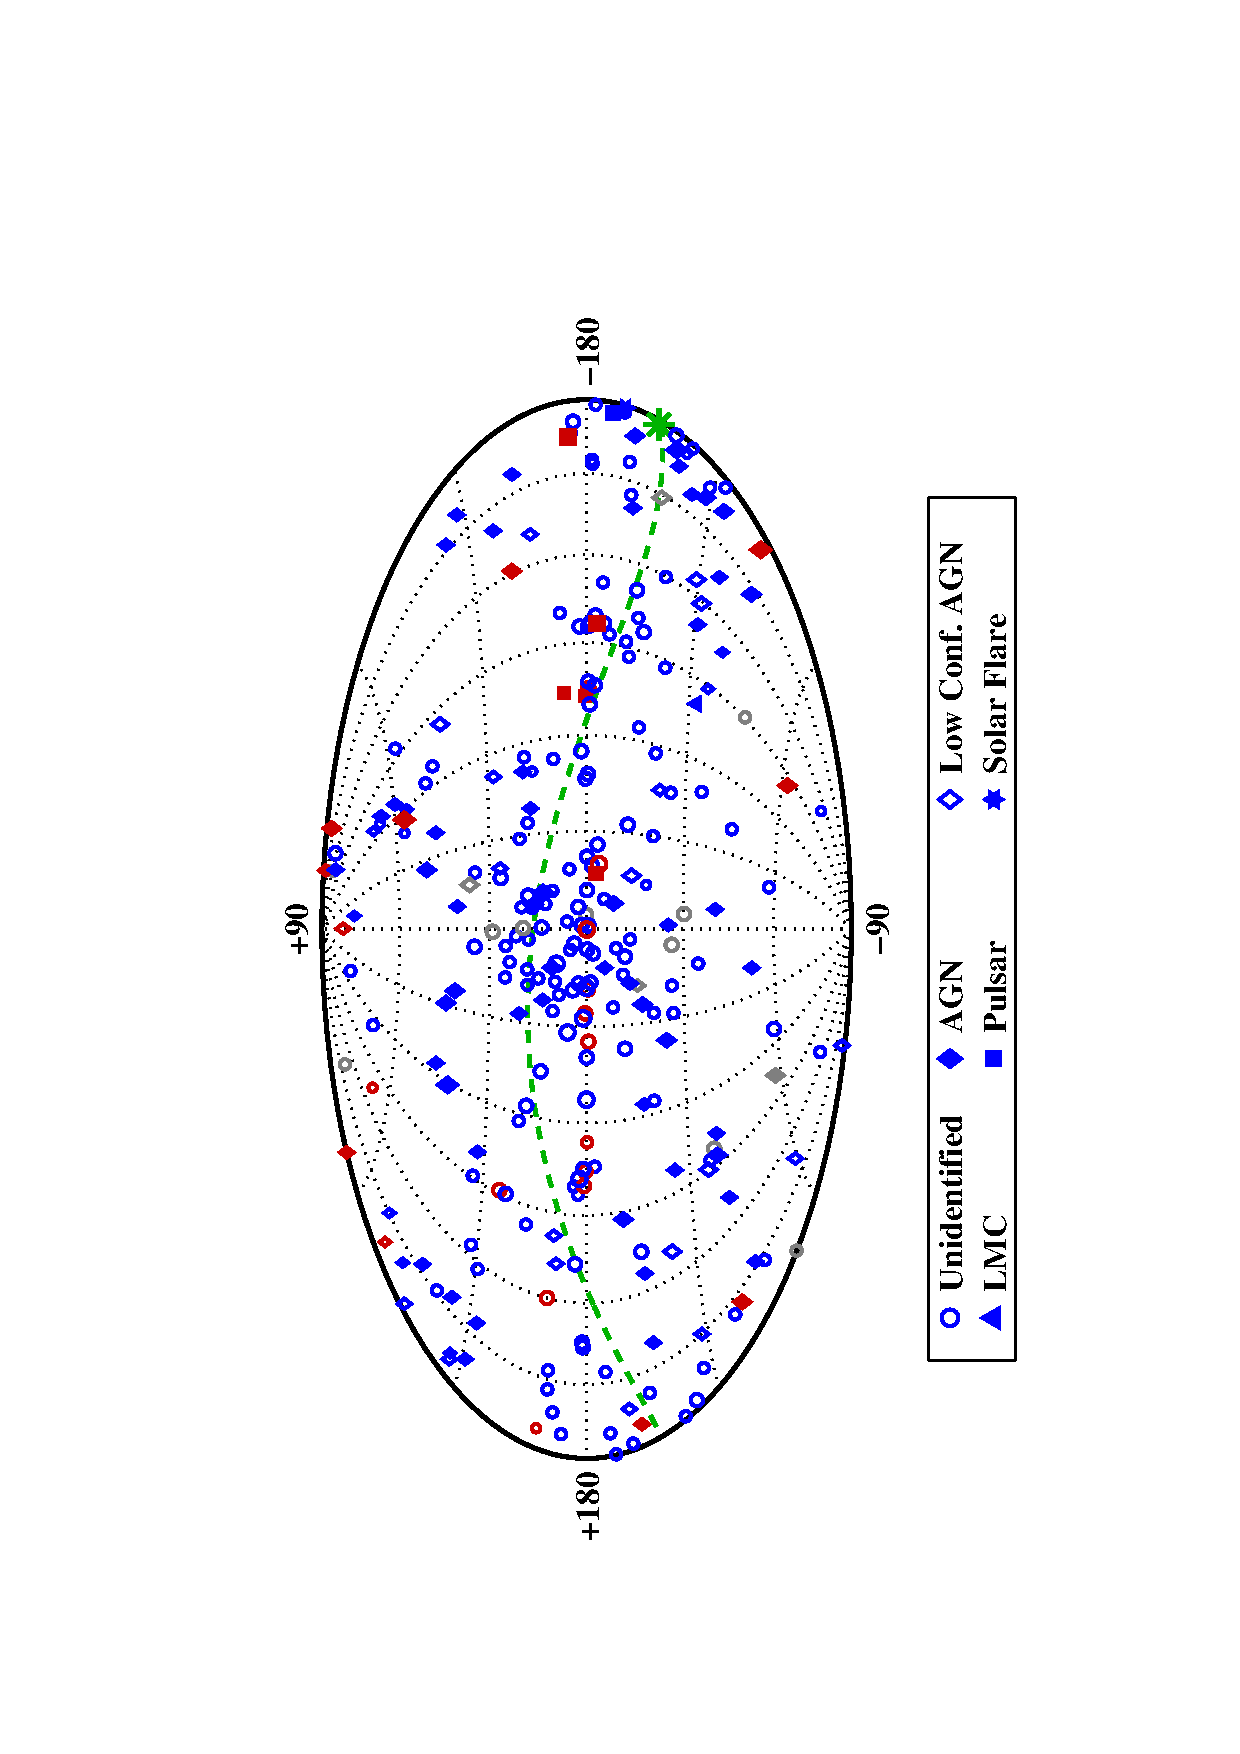
\includegraphics[angle=270,width=\textwidth]{plots/chap-introduction/3eg_catalog.pdf}
\caption{\label{FIG::INTRODUCTION::3RDEGRET} The 271 sources listed 
in the third EGRET catalog \citep{REF::HARTMAN::APJS1999}, plotted in
Galactic coordinates. Sources are displayed by source identification
(symbols) and flux (size of the symbol). Sources with a fitted
spectrum \textit{harder} than 2.0 are shown in red, those with a
softer spectrum are shown in blue. Those without an estimate of
spectral index are shown in gray. Finally, the Gould Belt is shown as
a broken green line, with the direction of the center of the Belt,
from \citet{REF::STOTHERS::AJ1974}, shown as a green star.}
\end{figure}

The catalog contains a total of 271 entries and upper limits on
emission for the remainder of the sky. For each source, maps of the
\textit{likelihood statistic}\footnote{In a likelihood analysis, the
likelihood statistic is analogous to significance. See
\citet{REF::MATTOX::APJ1996} for details.} are available, which give
the probability that the source is within a certain region of the sky at
various confidence levels.  The radius of 95\% confidence contour,
$\theta_{95}$, is quoted in the catalog as a bound on source
location. The average point source localization is
$\langle\theta_{95}\rangle=0.66^\circ$, large enough that the
error-box of many sources contains a large number of possible
counterparts at different energies, especially for those sources in
the region of the Galactic plane.

At low Galactic latitudes, 80 sources were listed in the 3EG
catalog. Five were definitively identified as known pulsars, one
corresponded to a solar flare and 74 had no unambiguous counterparts
at other energies. The 181 sources at $|b|>10^\circ$ include 66 likely
identifications with blazars, the Large Magellanic Cloud (LMC),
Centaurus A (a giant radio galaxy), 27 low confidence identifications
with AGN and 96 unidentified
sources. Figure~\ref{FIG::INTRODUCTION::3RDEGRET} shows the sources
in the 3EG catalog, by position on the sky, source type, flux
and spectral hardness.

\begin{figure}[t]
\includegraphics[draft=false,angle=270,width=\textwidth]{plots/chap-introduction/egret_ul.pdf}
\caption{\label{FIG::INTRODUCTION::3RDEGRETUL} 
Upper limits on \Gray emission at energies $>100$\,MeV from EGRET
observations, in units of $10^{-8}$\,cm$^{-2}$\,s$^{-1}$. As noted in
\citet{REF::HARTMAN::APJS1999}, the regions within $1^\circ$ of the
3EG sources are shown as black.}
\end{figure}

The majority of the detected sources are listed with flux estimates
from the viewing periods during which they were detected, and an
average flux over the full duration of the database. Many sources were
detected in each of the four viewing periods, some, such as the solar
flare, were only seen during certain portions of a single viewing
period. A systematic variability analysis of the EGRET data is
presented in \citet{REF::NOLAN::APJ2003}. Finally, the 3EG catalog
presents a power law fit to the spectrum of the detected \Grays for
those sources from which sufficiently large numbers of photons were
detected. For those parts of the sky in which no source was detected,
upper limits on emission at energies $>$100\,MeV were derived. The
limits, reproduced from the online version of the catalog, are shown
in figure~\ref{FIG::INTRODUCTION::3RDEGRETUL}. The limits represent
the maximum flux a source could have, at the 95\% confidence level,
without having been detected during the various observations by EGRET.

In addition to the third EGRET catalog, two catalogs of point-sources
detected by EGRET at higher energies have been produced. The
first, presented in two parts in \citet{REF::LAMB::APJ1997} and
\citet{REF::MACOMB::ICRC1999}, imposed a requirement that the
reconstructed energy of the \Gray be larger than 1\,GeV, and is
hereafter referred to as the GeV catalog. The production of this
catalog was motivated by the significantly smaller EGRET point spread
function at energies above 1\,GeV and by the lower background of
diffuse \Grays at these energies. It was hoped that sources could be
localized with improved accuracy and that sources with spectra harder
than the spectrum of background events would become more significant
at higher energies. A similar motivation guided the production of a
catalog of \Gray sources produced from those EGRET events with
energies greater than 10\,GeV
\citep{REF::DINGUS::GAMMA2001}, hereafter the 10\,GeV catalog. 

The first installment of the GeV catalog lists 57 sources at a
significance of $4\sigma$ and above. Ten of them had not been detected
at 100\,MeV energies in the \textit{second} EGRET catalog; a total of
thirty were listed as unidentified. The second installment of the GeV
catalog, which included data from all the EGRET viewing periods, added
another 16 sources with three that did not appear in the 3EG
catalog. The 10\,GeV catalog is based on a database of $\sim$1000
photons which were detected at large Galactic latitude; the catalog of
Galactic photons was presented at a conference but never appeared in
print. If it is assumed that the \Grays are uniformly distributed in
the sky, only two would be expected to be coincident with blazars by
chance within the EGRET point spread function. %A total of 23 photons
%were found to be coincident with AGN.

\section{Whipple 10\,m atmospheric \Cerenkov telescope}
\label{SEC::INTRODUCTION::WHIPPLE}

The Whipple 10\,m imaging atmospheric \Cerenkov telescope (IACT) is
located on Mt.~Hopkins in southern Arizona at an elevation of
2,300\,m. Built in 1968, it was the first dedicated \Gray instrument
of its type. In design, it has much in common with the large, fully
steerable, dish-type solar concentrators of the time and, indeed, it
was used as such for a brief period. For most of its life, though, it
has been operated as a ground-based \Gray telescope.  The telescope
can be operated by a single observer who chooses which sources to look
at, manages the data acquisition and analyzes the data to produce a
nearly real-time measurement of \Gray emission. The ability to produce
such a quick result has proved to be profitable on many occasions, by
prompting the telescope operator to continue to observe objects which
are in flaring states. The instrument is operated for 10 months of the
year, closing down during the summer to avoid lightning damage to the
sensitive electronics during the monsoon season.

The telescope has a total mirror area of $\sim$75\,m$^2$ and a focal
length of 7.3\,m. The mirror consists of an array of 249 identical,
spherical mirror facets, with radius of curvature 14.6\,m. The facets
are attached to a spherical optical support structure of radius
7.3\,m. This design, suggested by \citet{REF::DAVIESCOTTON::1957}, has
inferior on-axis performance when compared to a parabolic design but
has significantly improved off-axis characteristics. Since the
\Cerenkov light from an air-shower can be displaced from the direction
of the primary particle by the order of a degree or more, good
off-axis performance is important to IACT instruments. The design also
has the advantage that all mirror facets are identical and can be mass
produced. The mirrors are front aluminized at an in-house coating
facility, and anodized for protection from the environment. Front
coating improves the reflectivity in the UV band, where significant
\Cerenkov emission occurs, although it does leave the mirror coating
prone to weathering. The facets are aligned by hand at the end of each
monsoon season, and checked during the
year. Figure~\ref{FIG::INTRODUCTION::SCOPE} illustrates the design of
the telescope. As can be seen from the figure, the Davies-Cotton
design is not isochronous, a small time-spread is introduced between
parallel photons reflected from the center and edge of the mirror.

\begin{figure}[p]
\centerline{\includegraphics[height=0.4\textheight]{plots/chap-introduction/scope.pdf}}
\caption{\label{FIG::INTRODUCTION::SCOPE} Illustration of the Whipple 
10\,m telescope. The mirror consists of 249 spherical mirrors in a
Davies-Cotton configuration. The small time-spread introduced between
photons reflected from the edge and center of the mirror is evident
in the diagram.}
\end{figure}

A high resolution camera, consisting of an array of 379 1/2\,inch
phototubes in a close packed, hexagonal arrangement surrounded by 111
1\,inch phototubes, was installed on the instrument in 1999, see
figure~\ref{FIG::INTRODUCTION::PICS10M}. The PMTs have a quartz glass
window to extend their sensitivity into the UV. The voltage on each
channel is individually controllable with an Ethernet-based LeCroy
high-voltage system, allowing the gain on each channel to be equalized
across the camera. Signals from the inner 379 channels are transmitted
to the acquisition system on coaxial cables. Signals from the outer
channels are propagated on a prototype analog optical fiber system
designed to have very little dispersion. Due to the somewhat
experimental nature of the outer 111 tubes, data from them have not
been used in this survey. The inner, high resolution portion of the
camera has a field of view of $\sim2.2^\circ$.

\begin{figure}[p]
\hspace*{\fill}\includegraphics[height=0.25\textheight]{plots/chap-introduction/whipple99.jpg}\hspace*{\fill}\includegraphics[height=0.25\textheight]{plots/chap-introduction/G3Camera2_small.jpg}\hspace*{\fill}
\caption{\label{FIG::INTRODUCTION::PICS10M} Left: Picture of the
Whipple 10\,m telescope (courtesy of Dr.\ R.~Lessard). Right: Picture
of the high-resolution, 499 pixel camera at the focal plane of the
instrument. In normal operation, a reflective light concentrator
plate is installed over the face of the inner 379 PMTs to increase
photon detection efficiency -- the six mounting posts for this plate
are visible between the inner and outer parts of the camera.}
\end{figure}

The instrument is triggered when three neighboring channels exceed a
preset threshold within a given coincidence time. The signals from
each channel and other information, such as the absolute time of the
event from a GPS clock and time relative to the start of the data run,
are then stored on computer for off-line analysis. Details of the
trigger electronics and data acquisition system are given in
section~\ref{SEC::TECHNIQUE::ELECTRONICS}.

The data is analyzed off-line and a set of selection criteria (called
\textit{super-cuts}) are applied to discard $>98$\% of the background
events and retain $\sim50$\% of the \Gray events. From simulations, it
is estimated that the instrument has an effective area of
$4.4\times10^4$\,m$^2$ at 1\,TeV, after data selection has been
applied. For a source with a Crab-like power law spectrum,
$dN/dE\propto(E/TeV)^{-2.5}$, the energy at which the instrument
collects most {\Grayc}s, the \textit{peak response energy} is estimated
to be $E_\mathrm{peak}$=350\,GeV. The analysis technique is described
in chapter~\ref{CHAP::ANALYSIS}.

The relatively small field of view of the ground-based \Cerenkov
instruments dictates that observations be pointed in nature. In
general, they are targeted at prospective sources for a certain number
of hours in the hope of detecting emission. This is in contrast to
satellite instruments which tend to operate in a sky survey mode, at
least for the first few years of their life. There have been some
exceptions to this rule, such as the sky-survey performed with the
Whipple telescope before the adoption of the imaging technique
\citep{REF::WEEKES::ICRC1979} and the recent survey of the Galactic plane
region with the HEGRA telescope \citep{REF::AHARONIAN::AA2002}. 

\begin{table}[p]
\caption{\label{TAB::INTRODUCTION::INSTRUMENTS}
Comparison of the characteristics of the EGRET instrument on CGRO and
the Whipple 10\,m atmospheric \Cerenkov imaging telescope.}
\centerline{\begin{tabular}{lll}\hline
Characteristic & EGRET & Whipple \\\hline
Energy Range & & \\
(MeV) & 
\raisebox{1.5ex}[0pt]{30 to $3\times10^4$} & 
\raisebox{1.5ex}[0pt]{$3\times10^5$ to $3\times10^7$} \\[1.5ex]
%Energy Resolution & 20\% & 30\% \\
%($\Delta$E/E) & 100\,MeV to 2\,GeV & 300\,GeV to 10\,TeV \\[1.5ex]
Effective Area & 1200 at 100\,MeV & $2\times10^8$ at 350\,GeV \\
(cm$^2$) & 1600 at 500\,MeV & 
$4.4\times10^8$ at 1\,TeV \\
&  1400 at 3000\,MeV &
$3.6\times10^8$ at 10\,TeV \\[1.5ex]
Average error in & 5.85 at 100\,MeV & \\ 
% Whipple - Delta(Trans) = 0.29 / 0.10   Delta(Long) = 0.26 / 0.21
% Combined -- Delta(Combined) 0.275 @ 300GeV / 0.164 @ 1TeV
% => 68% containment = 1.5 x Delta(Combined) --- 0.41667 / 0.24849
\Gray origin -- $\theta_{68}$ & 1.71 at 1\,GeV & \raisebox{1.5ex}[0pt]{0.42 at 300\,GeV} \\
(degrees) & 0.50 at 10\,GeV & \raisebox{1.5ex}[0pt]{0.25 at 1\,TeV} \\[1.5ex]
Field of view & $\sim$0.6\,sr & 0.0012\,sr \\[1.5ex]
Sensitivity to Crab& $6\times10^{-8}$ $>$ 100\,MeV & 
$3.02\times10^{-11}$ $>$ 350\,GeV\\
like spectrum & (3$\sigma$ after 2 weeks & or 0.294 $\times$ Crab flux \\
% 2001/2002 crab rate - ON 13263, OFF 8949, TIME 94128.2 sec, EXCESS 4314
% SENSITIVITY IN 5HRS IS 0.3700 crab (5 sigma) / 0.2935 crab (4 sigma)
% Integral Crab-rate from Hillas et al. is I(>350 GeV)=1.03 x 10^-6/m^2/s
(cm$^{-2}$s$^{-1}$) & off Galactic plane) & (4$\sigma$ in 5\,hrs)\\\hline
\end{tabular}}
\end{table}

Table~\ref{TAB::INTRODUCTION::INSTRUMENTS} contrasts the
characteristics of the EGRET and Whipple instruments. Whipple has
considerably better point-source localization ability than EGRET and
has a field of view comparable to the average error-box of
unidentified sources in the 3EG catalog. The Whipple instrument has a
detection sensitivity of approximately 30\% of the Crab flux in 5
hours of observation -- given a required detection at the $4\sigma$
level. Figure~\ref{FIG::INTRODUCTION::SENSITIVITY} shows the
upper limit on the luminosity of an object\footnote{At a 99\%
confidence level, used throughout this survey.}, above 350\,GeV, which
can be derived from a \textit{non-source}, through observations of
0.5, 5 and 50 hours. The hypothetical EGRET source, is chosen to have
the mean flux and spectral index (and 1$\sigma$ errors on each) of the
sources chosen for this VHE survey.

\begin{figure}[p]
\centerline{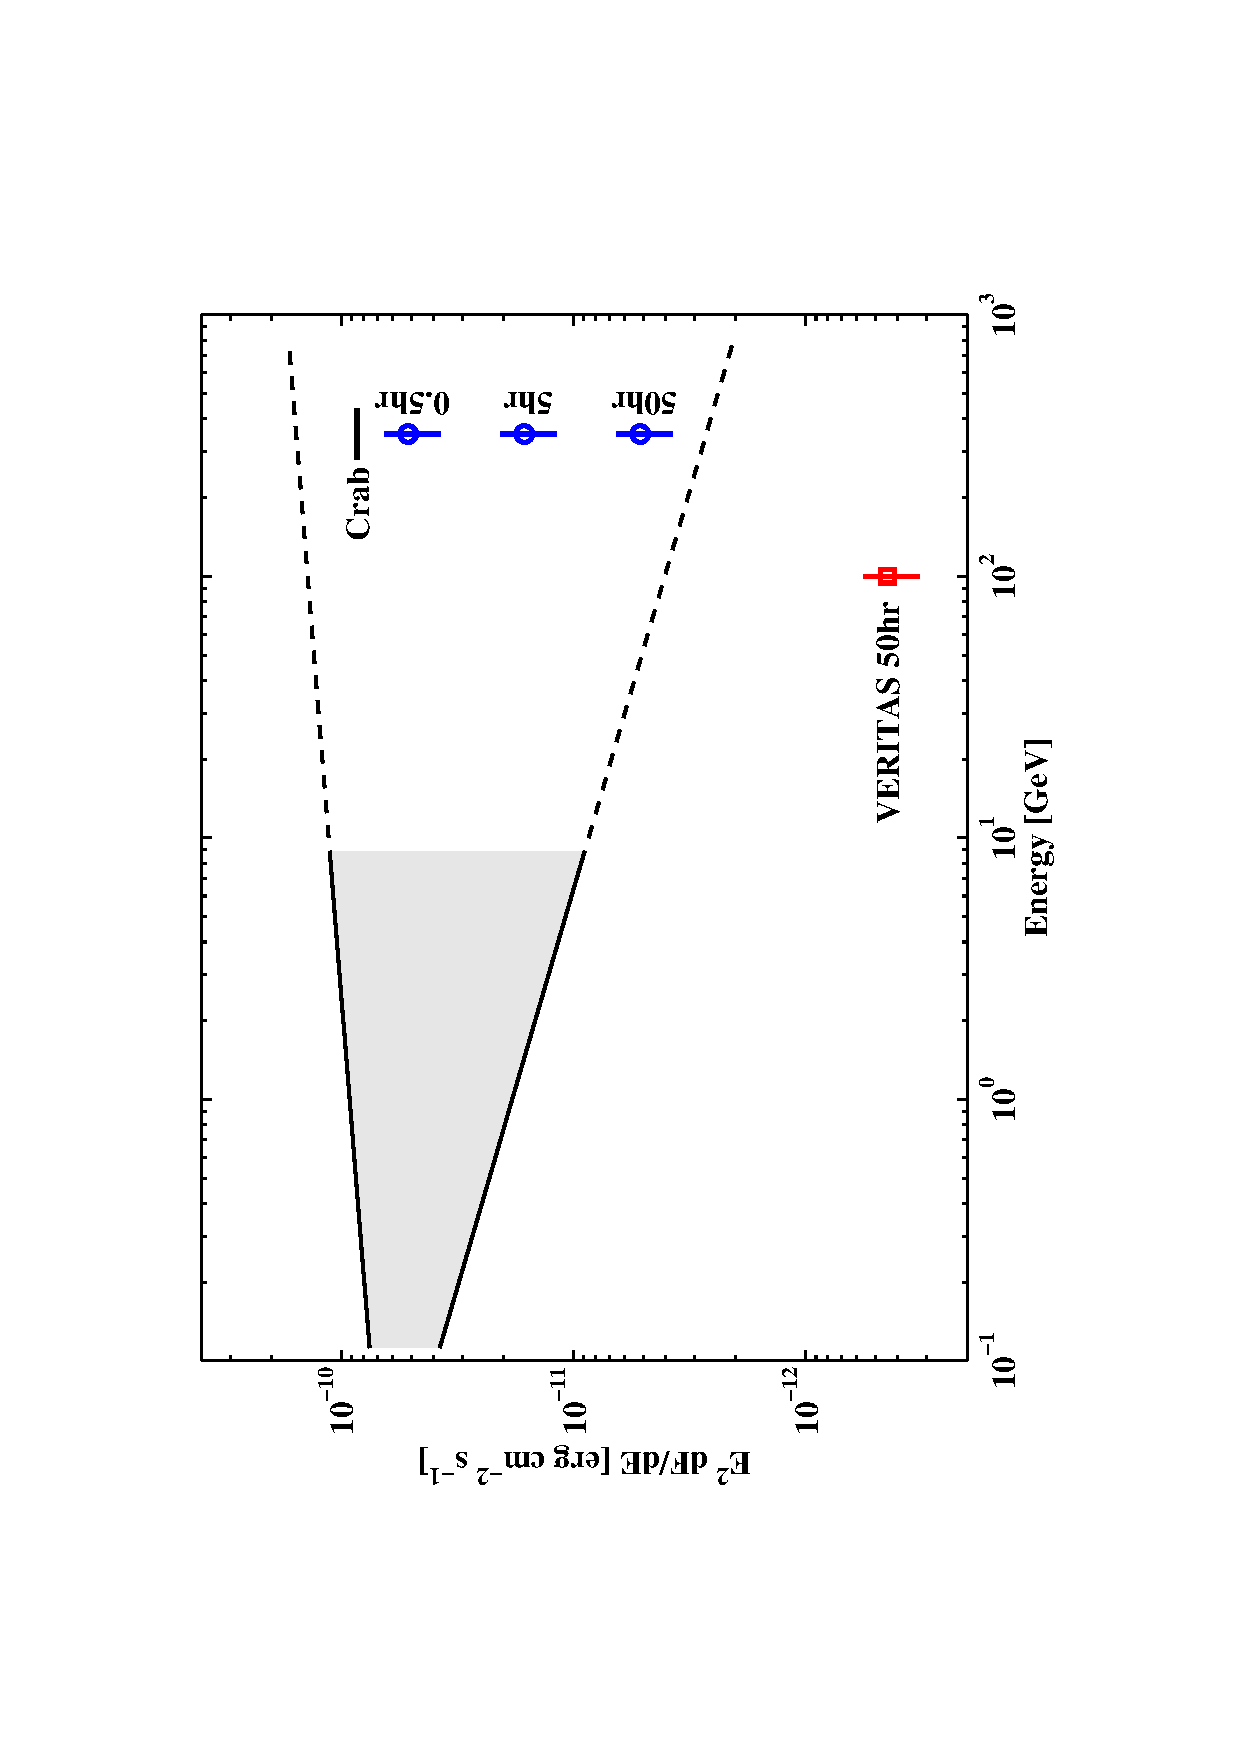
\includegraphics[angle=270,width=0.75\textwidth]{plots/chap-introduction/sensitivity_VHE_3eg_VERITAS.pdf}}
\caption{\label{FIG::INTRODUCTION::SENSITIVITY} 
Comparison of upper limit on source luminosity derivable through
observations at Whipple with the extrapolated luminosity of a ``mean''
100\,MeV source. Upper limits for 0.5, 5 and 50 hour observations are
shown, assuming a Crab-like spectrum. The hypothetical 100\,MeV
source, has an integral flux spectrum given by the mean flux and
spectral index from 3EG sources chosen for this survey:
$I(>E)=(30.9\pm4.1)\times10^{-8}(E/100MeV)^{-1.12\pm0.21}$\,cm$^{-2}$s$^{-1}$.}
\end{figure}

\section{Catalog of VHE gamma-ray sources}
\label{SEC::INTRODUCTION::VHECATALOG}

To date, 18 credible source detections have been made by ground-based
\Gray community. These sources are listed in
table~\ref{TAB::INTRODUCTION::VHESOURCES} and are plotted in
figure~\ref{FIG::INTRODUCTION::VHECATALOG}. Nine have been confirmed
by more than one ground-based instrument and are considered to be
beyond dispute. The others are, as yet, unconfirmed. In some of these
cases the discoveries are so recent that sufficient observations have
not been made by an independent group. In others cases it is because
there is no longer an independent telescope operating in the correct
range of latitude to provide confirmation. In the case of 3C66A, a
blazar discovered in 1998, it is possible that the initial discovery
was made during a period of extreme flaring activity, which has not
been repeated. In the case of Cen~X-3, flaring outbursts have been
noted at other wavelengths, but the VHE emission was reported to be
steady over the course of the observation. Since they are expected to
be persistent, and have not been confirmed, the discoveries of Vela
and Cen~X-3 have therefore been regarded as grade ``\textit{C}''
\citep{REF::HORAN_WEEKES::2NDVERITAS2004}.

\begin{table}[t] 
\caption{\label{TAB::INTRODUCTION::VHESOURCES}Catalog of published VHE 
sources$^1$. Adapted from \citet{REF::HORAN_WEEKES::2NDVERITAS2004}.}
\begin{centering}
\begin{tabular}{lllllll}\hline
Src.     & VHE catalog & Associated   & Source   & Discovery & 3EG     & Indep. \\
no.$^2$  & name      & source         & type & year/group$^3$& src.    & conf.  \\\hline
1  & TeV~0047$-$2518 & NGC 253        & Starburst  & 2003/C  & No      & No  \\
2  & TeV~0219$+$4248 & 3C66A          & Blazar     & 1998/Cr & Yes     & No  \\
3  & TeV~0535$+$2200 & Crab           & SNR/PWN    & 1989/W  & Yes     & Yes \\
4  & TeV~0834$-$4500 & Vela           & SNR/PWN    & 1997/C  & No      & No  \\
5  & TeV~1121$-$6037 & Cen X$-$3      & Binary     & 1998/D  & Yes     & No  \\
6  & TeV~1104$+$3813 & Mrk 421        & Blazar     & 1992/W  & Yes     & Yes \\
7  & TeV~1231$+$1224 & M87            & Radio Gal. & 2003/H  & No      & No  \\
8  & TeV~1429$+$4240 & H1426$+$428    & Blazar     & 2002/W  & No      & Yes \\
9  & TeV~1503$-$4157 & SN1006         & SNR        & 1997/C  & No      & Yes \\
10 & TeV~1654$+$3946 & Mrk 501        & Blazar     & 1995/W  & No      & Yes \\
11 & TeV~1710$-$4429 & PSR 1706$-$44  & SNR/PWN    & 1995/C  & No      & Yes \\
12 & TeV~1712$-$3932 & RXJ1713$-$3946 & SNR        & 1999/C  & No      & No  \\
13 & TeV~2000$+$6509 & 1ES1959$+$650  & Blazar     & 1999/TA & No      & Yes \\
14 & TeV~2032$+$4131 & \textit{unidentified} 
                       & \textit{unidentified}$^4$ & 2002/H  & Yes$^5$ & No  \\
15 & TeV~2159$-$3014 & PKS2155$-$304  & Blazar     & 1999/D  & Yes     & Yes \\
16 & TeV~2203$+$4217 & BL Lacertae    & Blazar     & 2001/Cr & Yes     & No  \\
17 & TeV~2323$+$5849 & Cas A          & SNR        & 1999/H  & No      & No  \\
18 & TeV~2347$+$5142 & 1ES2344$+$514  & Blazar     & 1997/W  & No      & Yes \\\hline
\end{tabular}

\footnotesize
\begin{tabular}{lp{0.95\textwidth}}
$^1$ & All VHE sources published in refereed journals are presented
here. Recent results from conferences, awaiting publication, are not
shown.\\ $^2$ & Source number from VHE source map,
figure~\ref{FIG::INTRODUCTION::VHECATALOG}.\\ $^3$ & C:~CANGAROO,
Cr:~Crimea, D:~Durham, H:~HEGRA, TA:~Telescope Array and W:~Whipple.\\
$^4$ & \citet{REF::BUTT::APJ2003} suggest that TeV~2032$+$4131 is
associated with an OB association, Cyg~OB2. Other associations have
also been made \citep{REF::MUKHERJEE::APJ2003}. \\
$^5$ & VHE source is coincident with 3EG~J2033$+$4118.
\end{tabular}
\end{centering}
\end{table}

\begin{figure}[t]
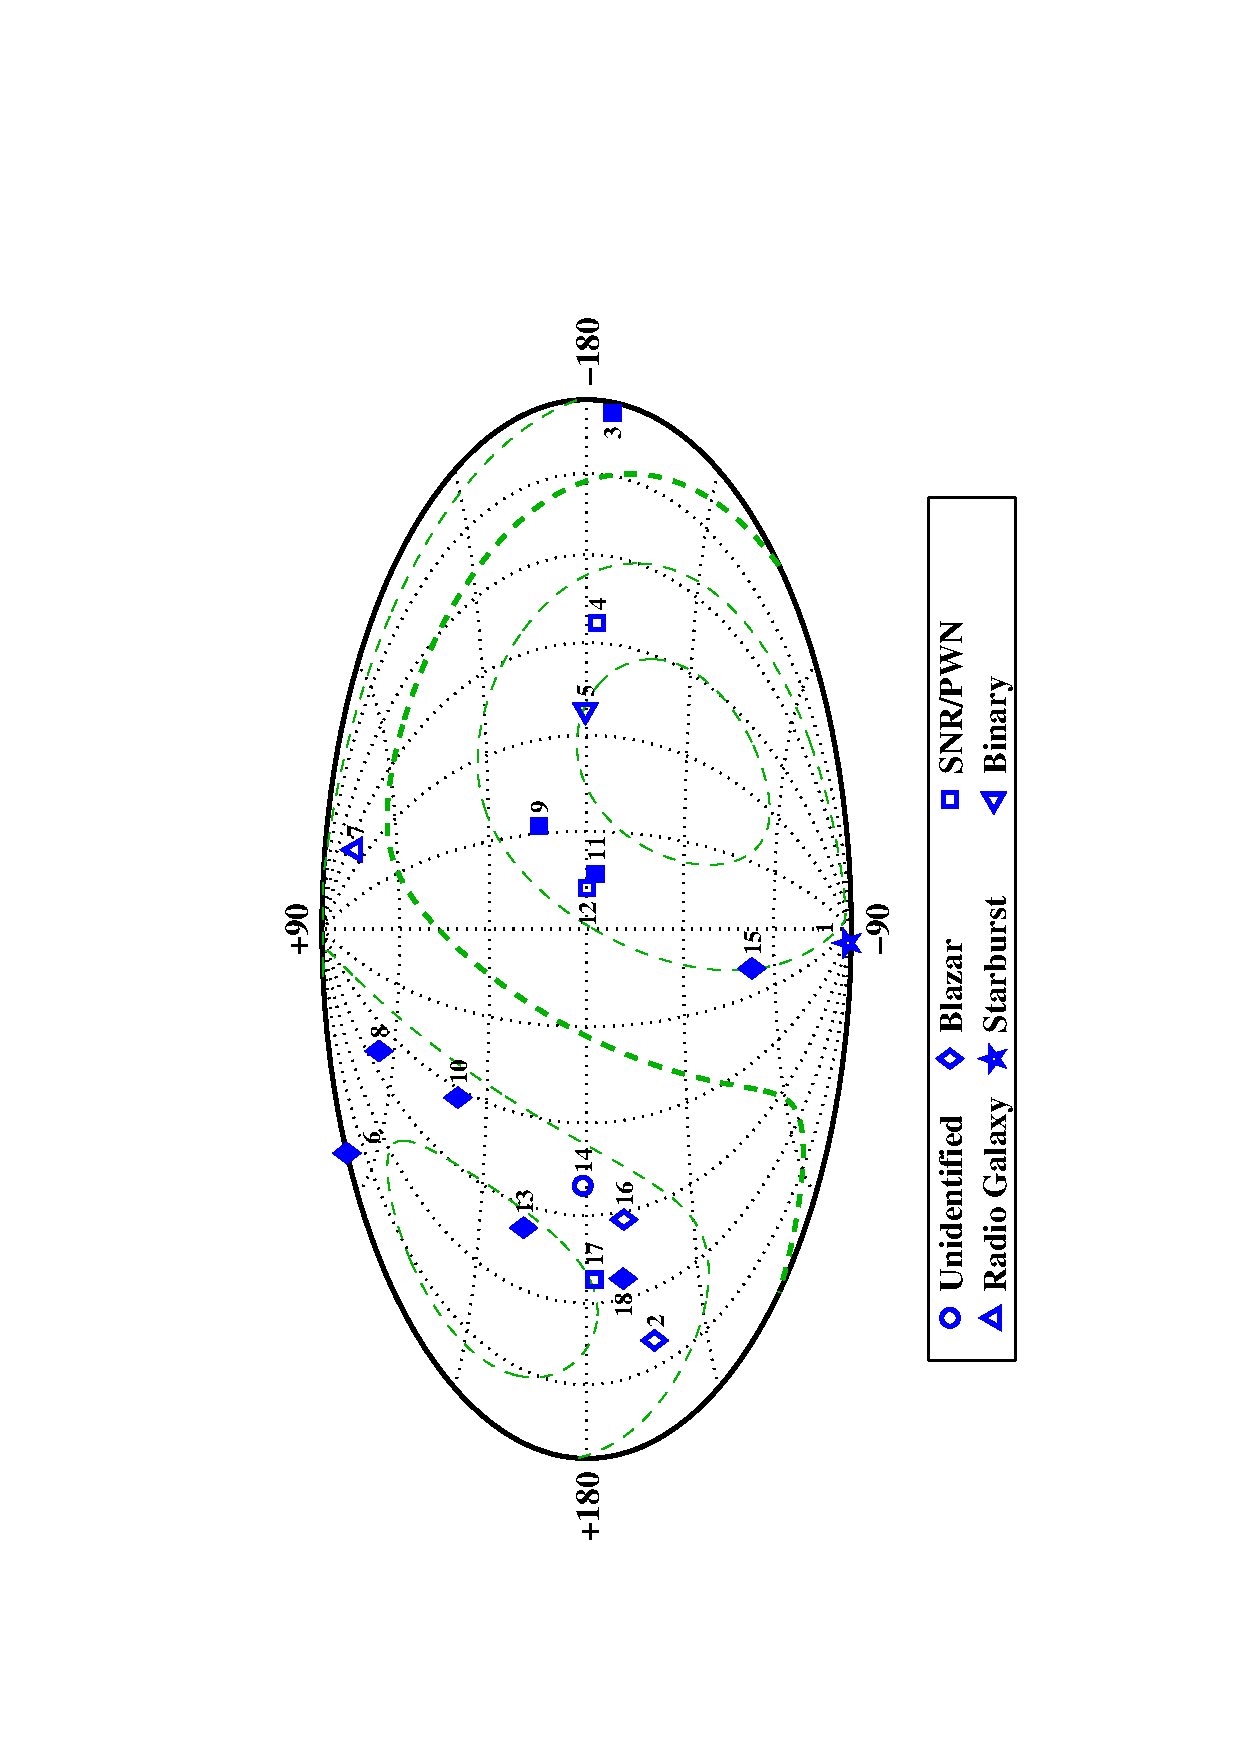
\includegraphics[angle=270,width=\textwidth]{plots/chap-introduction/tev_catalog.pdf}
\caption{\label{FIG::INTRODUCTION::VHECATALOG} 
The 18 objects reported as \Gray sources in the VHE regime, in
Galactic coordinates. Confirmed sources are depicted as solid symbols,
unconfirmed sources as outlines. Sources are listed by number, as they
appear in the VHE catalog, table~\ref{TAB::INTRODUCTION::VHESOURCES}. The
thick broken line shows the equatorial plane, separating the northern
and southern hemispheres. The thinner broken lines show the 30$^\circ$
and 60$^\circ$ declinations north and south. The data for this figure
are taken from \citet{REF::HORAN_WEEKES::2NDVERITAS2004}.}
\end{figure}

The mechanisms responsible for HE and VHE emission are discussed in
chapter~\ref{CHAP::SOURCES}. A brief list of the observational
characteristics of the sources and source types are presented below
without reference to the emission mechanisms.  

The first source detected by a ground-based \Gray instrument was the
Crab Nebula \citep{REF::WEEKES::APJ1989}. The Crab, a class of
supernova remnant (SNR) called pulsar wind nebula (or plerion -- see
section~\ref{SEC::SOURCES::PWN}), was the result of a historical
supernova explosion in the year 1054. It is a unique object, one of
the brightest in the sky over all wavelengths, with non-thermal
emission at radio, optical, x-ray and \Gray energies. Pulsations from
a central pulsar are seen at most energies up to and including the HE
\Gray range. The VHE emission from this object is consistent with
being steady over the 15 years for which it has been detected. It has
become the ``standard candle'' in the VHE regime, a source to
calibrate new instruments against. Its spectrum is well fitted by a
power-law with spectral index of $-2.49$ \citep{REF::HILLAS::1998}. No
periodicity has been seen in the VHE \Gray signal, which is not
thought to have come directly from the pulsar, but to emanate from a
synchrotron nebula surrounding it. In addition to the Crab, VHE
emission has been reported from two other pulsar wind nebulae, both in
the southern hemisphere: PSR~1706$-$44 and Vela.

The remaining SNR belong to the class of shell-type supernova
remnant. Two, SN1006 and RXJ1713$-$3946, are in the southern
hemisphere; the third, Cas~A, is in the northern hemisphere.  As
discussed in section~\ref{SEC::SOURCES::SNR}, SNR may be associated
with the acceleration of charged particles through diffusive shock
acceleration. The shape of the spectra of VHE \Grays from these
objects, in conjunction with observations at other wavelengths, is
expected to determine whether hadronic acceleration is occurring at
these sites, or whether the emission is the result of electron
acceleration. Emission from SN1006 is consistent with a purely
leptonic model, while RXJ1713$-$3946 and Cas~A may show evidence for
hadronic acceleration, see section~\ref{SEC::SOURCES::SNR}.

The VHE blazars, extra-galactic objects associated with compact
super-massive black holes (see section \ref{SEC::SOURCES::BLAZARS}),
are characterized by extreme variability on the time scales of hours
and days \citep{REF::GAIDOS::NATURE1996}. Their emission can go from a
quiescent state that is at or below the sensitivity of the Whipple
instrument to a flaring state with emission at a level of a few times
the Crab flux over the course of a single night of
observations. During these flaring periods, the spectral index of the
source has also been seen to change; in the case of Mrk~421, a
hardening of the spectrum from $-2.7$ to $-1.9$ was observed in
data from the Whipple telescope, taken during 2000/2001
\citep{REF::KRENNRICH::APJ2002}. Flaring activity at TeV energies 
is usually correlated with increased activity at other wavelengths, in
particular significant correlations with x-ray flares have been
observed \citep{REF::MARASCHI::AP1999}.

\section{VHE observations of third EGRET catalog sources}
\label{SEC::INTRODUCTION::VHE3EG}

The 170 unidentified sources in the 3EG catalog have motivated
multiwavelength studies at all wavelengths. Studies using the ASCA
x-ray satellite have revealed possible counterparts for some of them
\citep{REF::ROBERTS::APJS2001}, as have studies in the radio and
optical bands. In some cases, the multiwavelength approach has been
able to narrow the potential candidate associations, leaving a single
likely candidate. It is in the spirit of this tradition, that a survey
of unidentified sources has been undertaken with the Whipple VHE \Gray
telescope. The unidentified sources provide a catalog of objects whose
error-box is well matched to the field of view of an IACT. If VHE
emission is present, observations with an IACT would have sufficient
angular resolution to narrow down the potential candidates within the
error box of the 3EG source and, potentially, provide an unambiguous
association. This has been the scientific objective of the research
reported in this dissertation.

Objects have been chosen for the survey based upon a number of
factors. Preference was given to persistent objects, with hard spectra
for which a lack of VHE emission would necessitate a cut-off in the
spectrum. In all cases, the location of the source in the sky
influenced the choice. It is desirable that sources lie between
declinations of $10^\circ$ south and $70^\circ$ north so that they are
can be observed with the Whipple telescope at relatively small angles
from the zenith, for which the density of \Cerenkov photons on the
ground is highest. Additionally, since the telescope is operated by a
relatively large collaboration, with diverse research interests,
sources were chosen so as not to clash with areas of the sky for which
considerable conflicting interests exist, such as the Galactic Center
region. Finally, \citet{REF::PETRY::NUGH2001} extrapolated the known
EGRET spectrum of the unidentified sources to provide a table of most
likely detections with next-generation \Cerenkov instruments. A number
of the most likely sources from this list were
chosen. Chapter~\ref{CHAP::OBSERVATIONS} lists the 3EG sources chosen
in this survey and presents the results of the VHE survey.

\chapter{Potential sources of high-energy gamma-rays}
\label{CHAP::SOURCES}

To date, EGRET sources have been unambiguously identified with only
two major source types: blazars and pulsars (neglecting the LMC, Cen
A, the solar flare and \Gray bursts). Numerous population studies have
noted that there are coincidences between the population of
unidentified sources and catalogs of other types of sources which
exceed what should be expected from chance probability; however these
studies do not provide compelling associations for any individual 3EG
sources. Some suggested source classes are massive stars, OB
associations, supernova remnants (SNR), x-ray binaries and
micro-quasars. In addition, it seems likely that there are three
independent populations of unidentified source: those associated with
the Galactic plane, extra-galactic sources and a population of local
sources in the Gould Belt.

\section{Blazars}
\label{SEC::SOURCES::BLAZARS}

One of the most unexpected results from the EGRET mission was the
discovery of \Grays from a large number of extra-galactic
sources. Before EGRET, only one extra-galactic source had been
detected in {\Grayc}s, 3C273, based upon observations with the COS-B
satellite \citep{REF::SWANENBURG::NATURE1978}. In total, 67
high-confidence associations of EGRET sources were made with blazars,
a type of radio loud active galactic nucleus (AGN). AGN are galaxies
with a bright central core which typically outshines the $\sim10^{11}$
stars present in the Galaxy by up to three orders of magnitude. AGN
are thought to be powered by accretion of material onto a
super-massive black hole, (mass $\sim10^6M_\odot$ to
$\sim10^{9}M_\odot$). The accreting material forms a disk around the
core, at temperatures which can produce continuum emission at UV to
soft x-ray energies. AGN can form jets of relativistic charged
particles, aligned perpendicular to the plane of the accretion
disk. The mechanism responsible for forming the jet is not completely
understood. The accretion disk is surrounded by clouds of hot gas
which produce broad line emission. Far out from the core, narrow line
emission is produced in clouds of particles, possibly energized by the
jet.

AGN have been sub-classified based upon their observational
properties, with some classes being more powerful, and therefore
better studied, in different energy ranges. At \Gray energies, the
blazar subclass of AGN are powerful emitters. Blazars are
characterized by strong emission in radio (they are referred to as
radio-loud AGN), continuum emission across the spectrum, very rapid
variability on the order of hours to days and weeks, high polarization
and the ejection of ``blobs'' of material at apparent super-luminal
velocities, usually visible in radio. The blazar sub-class consists of
``BL Lac'' type objects, and flat-spectrum radio quasars
(FSRQs). These objects are distinguished on the basis of prominent
(FSQR) or weak (BL Lac) absorption/emission lines in their spectra. In
general, the lack of lines in the spectra of BL Lac objects makes it
difficult to determine their redshift, and hence distance. It also
means that they are usually identified as AGN at radio or x-ray
energies, since they are essentially featureless at optical
wavelengths. It has been suggested that all AGN can be unified by a
single model
\citep{REF::URRY::PASP1995}, and that the different observational
properties of the AGN classes arise primarily from differences in the
viewing angle with respect to the jet and the total power of the
accreting object. For example, the presence or absence of broad lines
in the spectrum depends on whether the broad line emission region is
obscured from sight by other parts of the AGN structure. Blazars are
thought to be AGN with jets aligned close to our line-of-sight. The
physics behind \Gray emission in the jet is not well known, and many
models exist. The most widely discussed models are leptonic,
synchrotron/inverse Compton models, in which synchrotron emission from
electrons in the jet produces the low energy emission (radio, optical
and soft x-ray) while inverse Compton up-scattering of the soft
synchrotron photons by the same population of electrons accounts for
the high energy emission. This model, referred to as the
synchrotron-self-Compton (SSC) model, predicts that the peak in the
power output of the IC component is correlated with the peak in the
synchrotron emission, and has been relatively successful in fitting
the emission seen from blazars. A review of leptonic emission models
can be found in \citet{REF::BOETTCHER::1999SNOWBIRD}.

The identification of some EGRET sources with blazar objects is
presented in detail in \citet{REF::VONMONTIGNY::APJ1995},
\citet{REF::MUKHERJEE::APJ1997}, \citet{REF::HARTMAN::APJS1999} and
references therein. A recent summary of the EGRET blazars can be
found in \citet{REF::MUKHERJEE::HEGRA2001}. In general,
identifications were made on the basis of positional coincidence with
known radio sources.  The blazars listed in the 3EG catalog consist
of 50 FSRQs and 17 BL~Lacs, with redshift between $z=0.03$ and
$z=2.28$. For most of these objects the \Gray emission dominates the
total luminosity at all other wavelengths. Their spectra are well fit
by a power-law with average spectral index of
$\langle\Gamma\rangle=2.2$ and no cut-off has been seen up to
10\,GeV. The average variability index of the blazars, from
\citet{REF::NOLAN::APJ2003}, is $\langle\delta\rangle=0.70\pm0.08$
with $\mathrm{RMS}(\delta)=0.27\pm0.05$, showing that they are
consistent with being variable ($\delta\rightarrow0$ for persistent
sources, and $\delta\rightarrow1$ for variable sources).

The GeV and 10\,GeV catalogs also contain a number of additional
blazar identifications. The 10\,GeV catalog suggests that there may be
a blazar identification for 3EG~J0433$+$2908 and for GeV~J0508$+$0540.  In
the time since the 3EG-catalog was published a number of
investigations have been made into individual unidentified EGRET
sources, leading to possible (or likely) blazar identifications for
them. For example, \citet{REF::MUKHERJEE::APJ2000} suggest that
3EG~J2016$+$3657 is associated with a blazar, an especially interesting
result as the source is located at low Galactic latitude
($b=0.5^\circ$), possibly making it the first blazar identified in the
direction of the plane.
% Could mention Wallace 2002 see wallace-agn-J2006-2321-01.pdf

Of the 3EG blazars, two are confirmed sources of VHE {\Grayc}s:
Markarian~421 (usually abbreviated to Mrk~421) and PKS2155$-$304. A
third confirmed VHE source, Mrk~501 is significant only in the EGRET
GeV catalog. On the other hand, there are three confirmed VHE blazars
not seen by EGRET: H1426$+$428, 1ES1959$+$650 and 1ES2344$+$514, all
BL Lac type objects. To date, no FSRQs have been detected by VHE
instruments. EGRET largely detected low-frequency peaked BL~Lacs (LBL)
and FSRQs. These objects have the peak in their synchrotron power
emission in the optical, UV or soft x-ray bands. All confirmed BL~Lac
detections in the VHE band are high-frequency peaked BL~Lacs (HBL),
with peak synchrotron power in the hard x-ray band. Correspondingly,
the peak in the inverse Compton emission is at higher energies in
HBLs, lying in the 300\,GeV to 30\,TeV range. The energy range in
which EGRET was most sensitive fell in that region of the spectrum in
which HBLs are least powerful; between the peaks of the synchrotron
and inverse-Compton emission. Therefore, EGRET was not sensitive
enough to detect many of the TeV selected BL~Lacs. The most distant
blazar detected in the VHE regime is H1426$+$428, at a redshift of
$z=0.129$. Many models predict that interactions of VHE \Grays with
the extra-galactic background light will attenuate the \Gray signal to
such an extent that sources located at distances much larger than
H1426$+$428 are not be visible in \Grays at GeV-TeV energies, with
current detector sensitivities.

In summary, it seems likely that blazars make up a considerable
fraction of the unidentified EGRET sources. Blazars are expected to be
uniformly distributed across the sky, to have flat spectra which
steepen with distance, and are characterized by extreme variability
across the spectrum from radio to TeV energies. Since the known \Gray
blazars have been readily identified with their radio, optical and
x-ray counterparts, new identifications would suggest some unusual
spectral distributions and/or obscuration, e.g.\ by the Galactic plane.

\subsubsection*{\boldmath Intergalactic \Gray absorption}

The spectra of \Grays detected from all extra-galactic sources are
altered from the intrinsic source emission spectrum by absorption of
the signal in the ambient field of intergalactic
photons. \citet{REF::NIKISHOV::JETP1961} was the first to suggest that
high-energy photons would interact with infra-red photons in
intergalactic space by photon-photon pair production. At that time,
little was known about the strength of the inter-galactic infra-red
radiation field (IIRF) and the value assumed in the calculation was
too large by three orders of magnitude. Shortly after the discovery of
the cosmic microwave background (CMB), it was realized by
\citet{REF::GOULD_SCHREDER::PRL1966} and \citet{REF::JELLEY::PRL1966}
that the universe is effectively opaque to \Grays with energy greater
than $\sim$100\,TeV. \citet{REF::GOULD_SCHREDER::PR1967} extended these
calculations to account for absorption with radio, microwave, IR and
optical photons.

The unexpected discovery of the optically violent variable quasar,
3C279, by EGRET prompted \citet{REF::STECKER::APJ1992} to suggest that
any subsequent discovery of TeV emission from the object could be used
to determine (or at least provide limits on) the density of the
IIRF. The discovery of the blazar Mrk~421 at TeV energies
\citep{REF::PUNCH::NATURE1992}, and the subsequent discovery of other
TeV blazars, has produced considerable interest in this subject
\citep[see for example][and references
therein]{REF::VASSILIEV::AP2000}.

\enlargethispage{13pt}
The threshold for a a soft photon with energy $\epsilon$ (as measured
locally) to interact with a \Gray with energy $E$ (measured locally)
at redshift of $z$ is \[\epsilon>\frac{2(m_ec^2)^2}{E(1+z)^2}
\approx\frac{0.52}{E/\mathrm{TeV}}\,\mathrm{eV.}\] for small
redshifts. For a 1\,TeV photon, this corresponds to an IR photon near
to the K-band (2\,$\mu$m). For energies above 100\,TeV the threshold
is in the CMB region. The amount of absorption a signal from a distant
source undergoes can be calculated from the pair-production
cross-section, due to Heitler, given some assumptions for the spectrum
of soft-photons \citep[see for
example][]{REF::STECKER::SSR1996}. \citet{REF::STECKER_DEJAGER::AA1998}
calculated the optical path length (or \textit{opacity}, $\tau(E,z)$)
for TeV photons from relatively small redshifts ($z\leq0.3$), which
they presented in parameterized form, valid for 1\,TeV$<E<$50\,TeV and
$z<0.3$. Figure~\ref{FIG::SOURCES::EBL} shows the opacity, from the
parameterized form, as a function of \Gray energy for three
redshifts. The change in the intrinsic source spectrum for these cases
is also shown. In each case a strong cut-off\,\footnote{Defined as the
energy at which $\tau(E,z)=1$ and the spectrum falls to 1/e of its
intrinsic value.} in the measured \Gray spectrum is predicted,
independent of the source emission spectrum. For sources at
$z\sim0.03$, like Mrk~421, the cut-off occurs at $\sim10$\,TeV,
decreasing to $\sim1$\,TeV for a more distant source, such as
H1426$+$428 at $z=0.129$.

\begin{figure}[t]
\hspace*{\fill}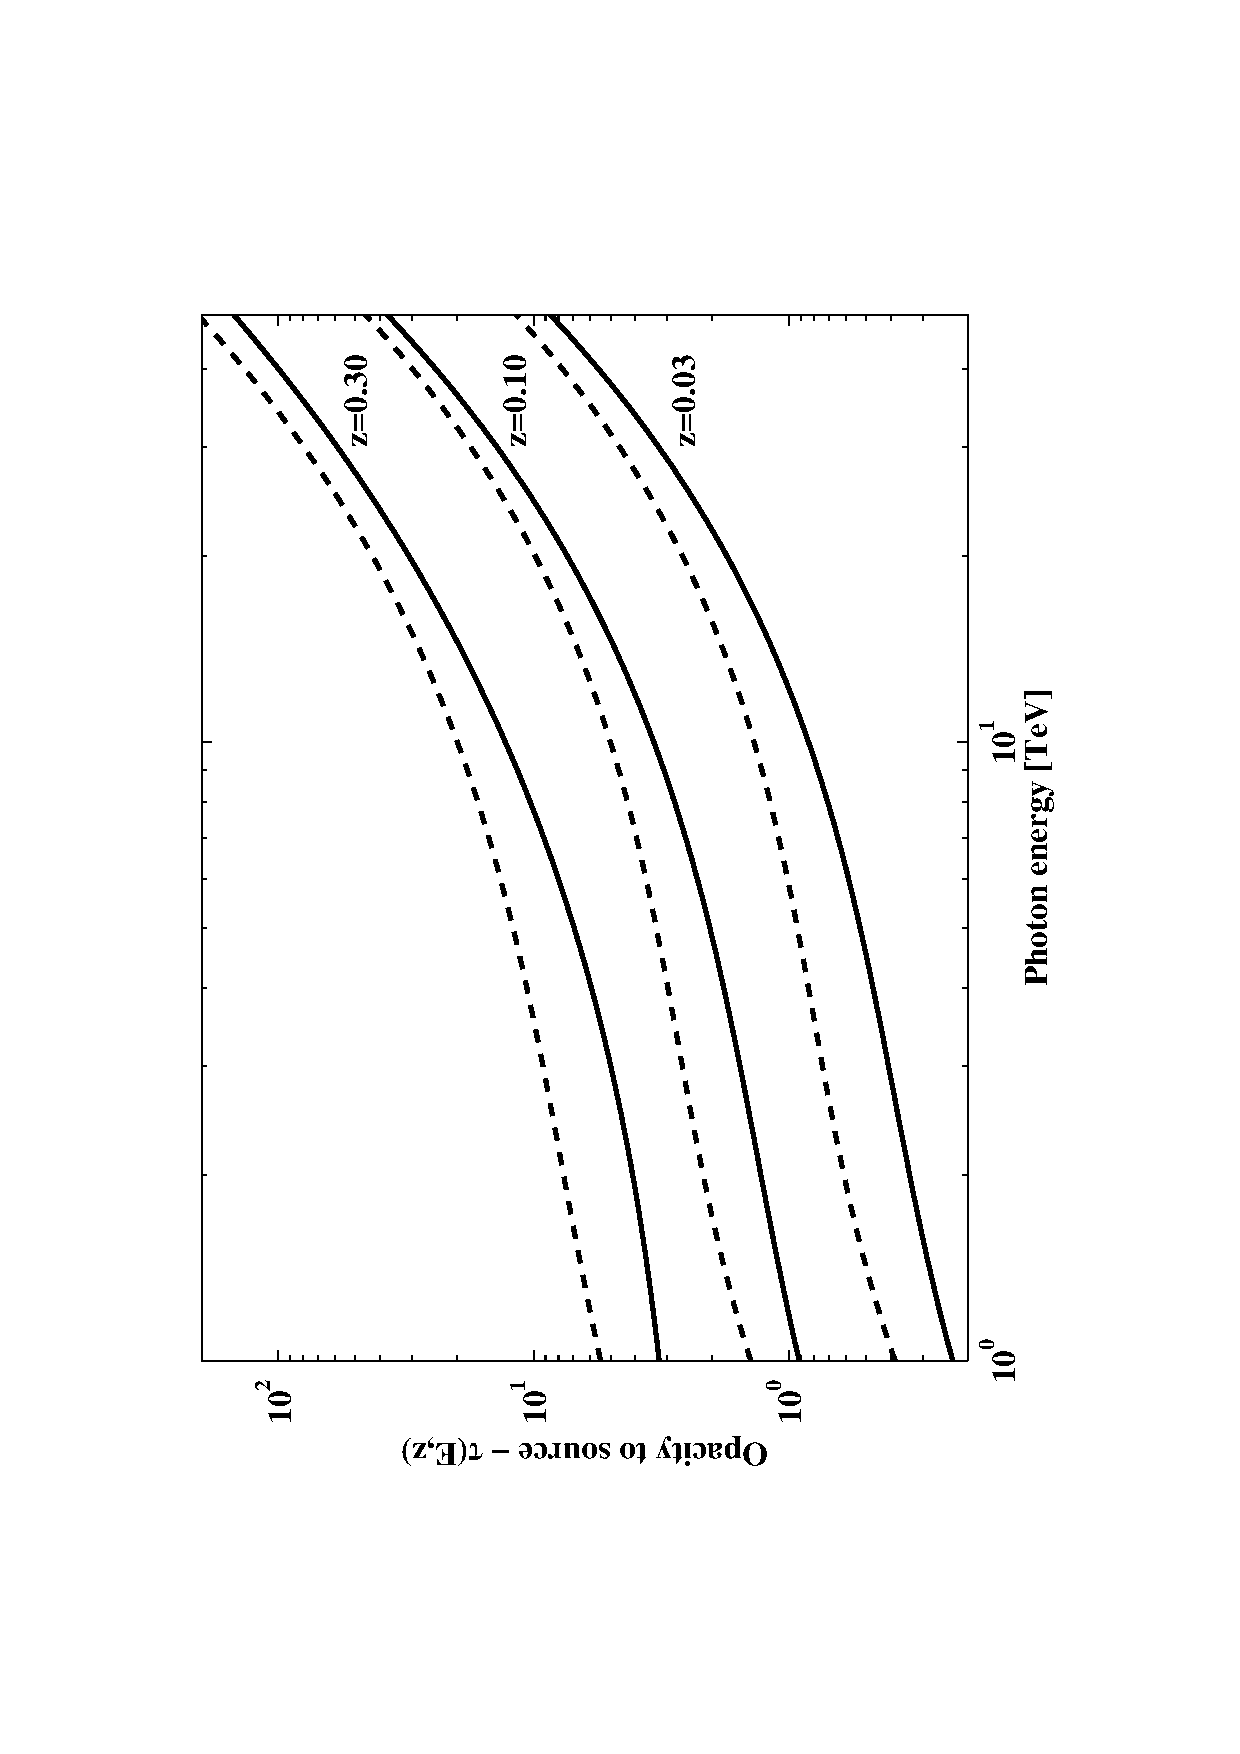
\includegraphics[angle=270,width=0.49\textwidth]{plots/chap-sources/ebl_opacity.pdf}\hspace*{\fill}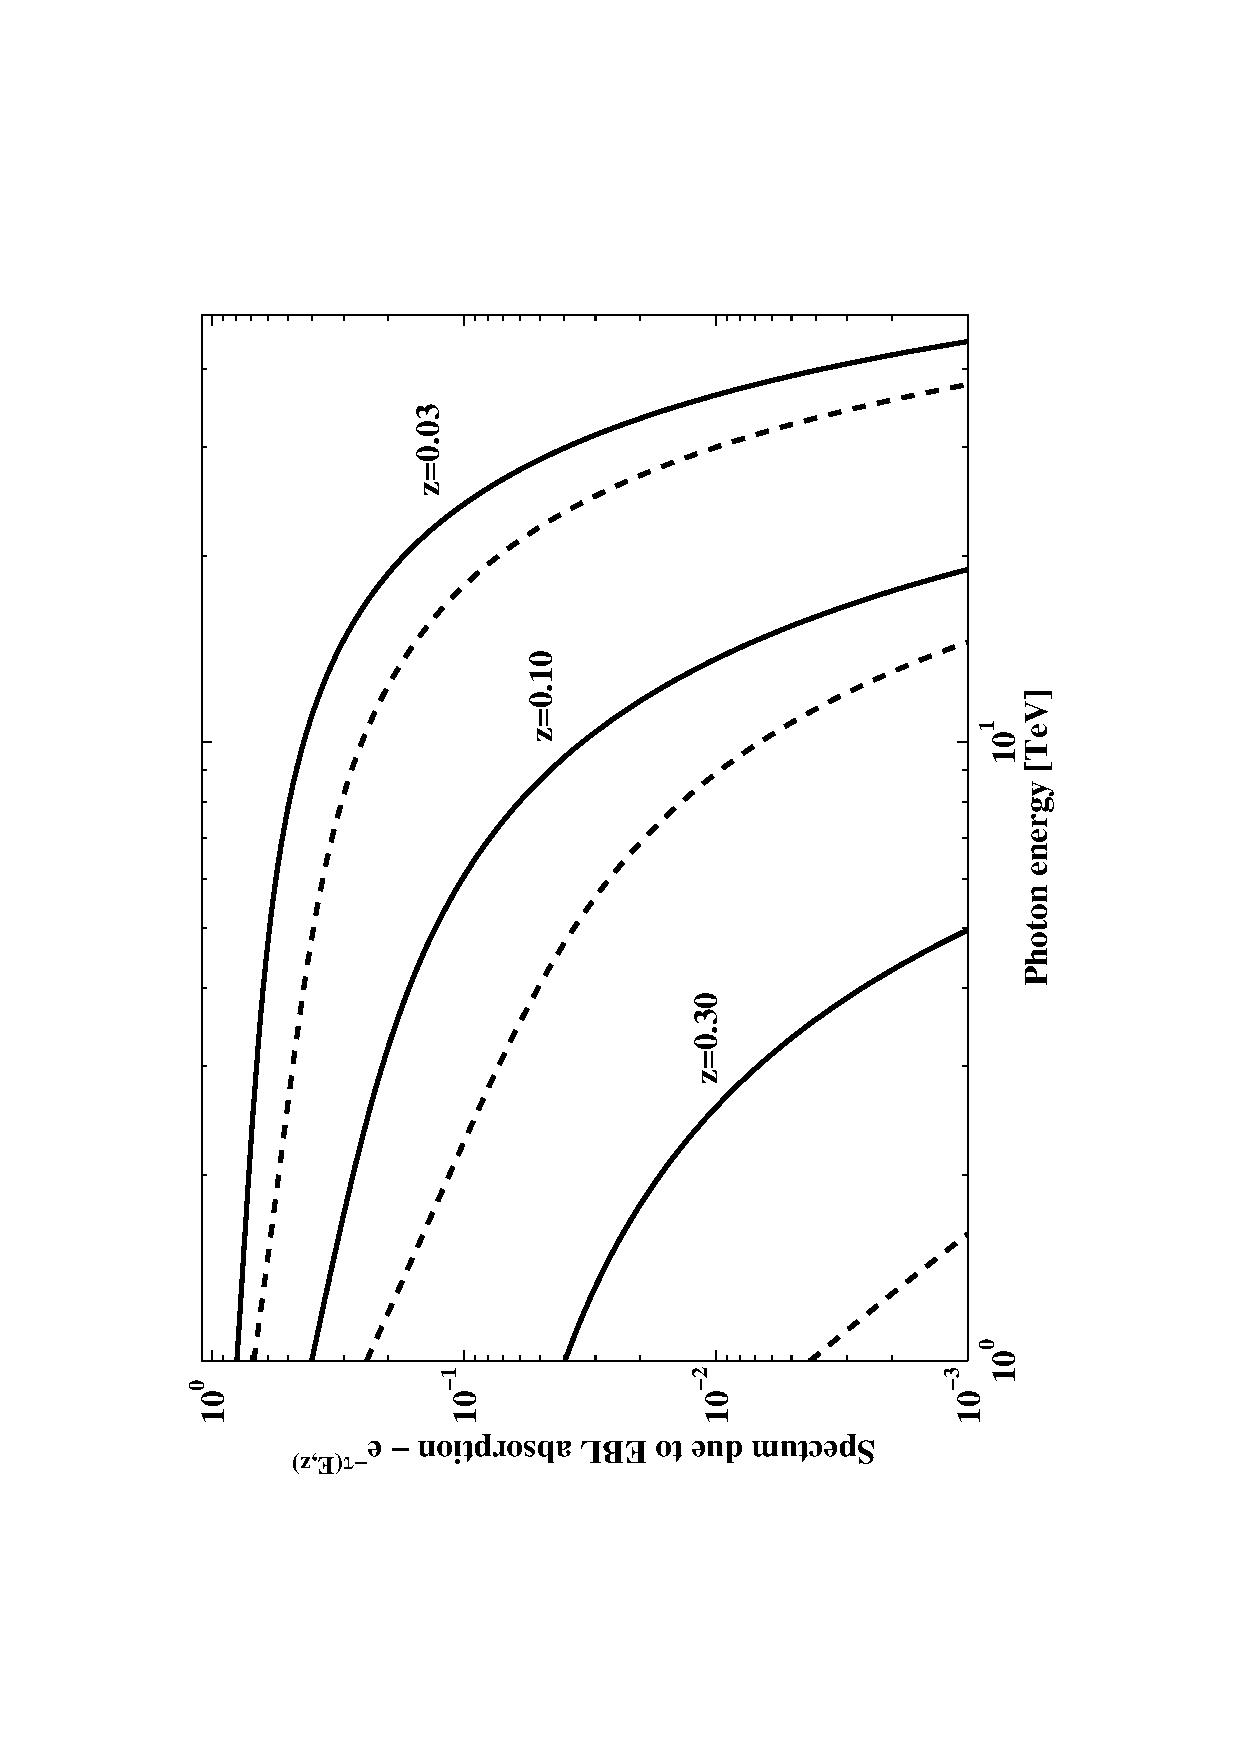
\includegraphics[angle=270,width=0.49\textwidth]{plots/chap-sources/ebl_spectrum.pdf}\hspace*{\fill}
\caption{\label{FIG::SOURCES::EBL} (Left) Optical path length, $\tau(E,z)$,
for HE \Grays from extra-galactic sources at $z=0.03$, $z=0.10$ and
$z=0.30$ from \citet{REF::STECKER_DEJAGER::AA1998}. (Right) Cut-off in
\Gray spectrum due to absorption, $\exp\{-\tau(E,z)\}$. In each case,
two curves are shown, corresponding to the two the IIRF models used by
\citet{REF::STECKER_DEJAGER::AA1998}.}
\end{figure}

Predicting VHE emission from the EGRET blazars requires the
opacity be known in the energy range $\sim$1\,GeV$<E<\sim$1\,TeV, and
for larger redshifts. For this energy range, the extra-galactic soft
photon spectrum must be estimated at optical wavelengths, where the
major contribution comes from
starlight. \citet{REF::SALAMON_STECKER::APJ1998} presented a
calculation of this function, and its implication for a number of
EGRET blazars. They did not present a parameterized form of the
function, which could be plotted here. Qualitatively, the results are
similar to the TeV case: the opacity increases with energy and
redshift. For a source at $z=1$ the opacity increases from $<10^{-2}$
at 20\,GeV to $\geq8$ at 500\,GeV. For the EGRET source 3C279
($z=0.54$) a spectral cut-off is predicted at $\sim$90\,GeV; for B1633$+$382
($z=1.81$) it is at $\sim$25\,GeV.

\section{Pulsars}
\label{SEC::SOURCES::PULSARS}

\enlargethispage{8pt}
The second largest category of identified MeV \Gray point sources is
pulsars. The 3EG catalog lists five associations between pulsars and
EGRET point sources: Crab, Vela, Geminga, PSR~B1706$-$44 and
PSR~B1055$-$52 \citep{REF::NOLAN::AAS1996}.
\citet{REF::KASPI::APJ2000} report evidence of pulsations from
PSR~B1046$-$58 (3EG~J1048$-$5840) at the $3.1\sigma$ level. PSR~B1951$+$32,
was identified as a pulsar in EGRET data
\citep{REF::RAMANAMURTHY::APJ1996}, although it does not appear in the
3EG catalog\footnote{The pulsar is depicted at the correct location in
the map of sources, figure~4, in
\citet{REF::HARTMAN::APJS1999} while it is missing from
figure~\ref{FIG::INTRODUCTION::3RDEGRET} in
chapter~\ref{CHAP::INTRODUCTION}, which was generated directly from
the electronic version of the 3EG catalog.} (it fell below the
$5\sigma$ requirement for detection on the Galactic
plane). \citet{REF::RAMANAMURTHY::APJ1995} present results of
pulsations from PSR~B0656$+$14 at the $3.6\sigma$ level, although
again it is not a 3EG source. In an interesting analysis of a source
that contains two possible candidates, \citet{REF::KUIPER::AA2000}
show evidence for pulsations from PSR~J0218$+$4232 at the 3-4$\sigma$
level which is coincident with 3EG~J0222$+$4253, with sufficient \Gray
excess remaining to also accommodate the detection of the blazar 3C66A
in that field. \citet{REF::HALPERN::APJ2001::2227PAPER2} report
observations of the region near 3EG~J2227$+$6122 in x-ray, optical and
radio and suggest an association with an x-ray/radio pulsar
PSR~J2229$+$6114. Lacking an appropriate ephemeris covering the EGRET
observations, they were not able to perform a pulsed search at MeV
energies -- but, since no other x-ray counterpart is found to be
consistent, they claim it is more conservative to accept the
association than to reject it. Finally, PSR~B1509$-$58 is also a \Gray
pulsar; pulsations have been detected at lower energies by the OSSE
and BATSE experiments on CGRO but not by EGRET
\citep{REF::ULMER::APJS1994}.

The unambiguous associations, listed above, were made by searching for
significant pulsations in the \Gray data, given a contemporaneous
pulsar ephemeris (phase, frequency and frequency derivatives), usually
determined from radio observations\footnote{Or from ROSAT x-ray
observations in the case of the radio-quiet Geminga
pulsar.}. Additionally, blind searches for pulsations were performed
for those sources with sufficient detected counts. The median number
of counts detected from unidentified sources on the plane is
$\sim400$, insufficient for a blind search considering that the
PSR~B1046$-$58, $3.1\sigma$ identification was made with $\sim350$
counts and a \textit{known} pulsar ephemeris.

Since mid-1997, the sensitive Parkes Multibeam Survey
\citep{REF::MANCHESTER::MNRAS2001} has detected a large number of new
radio pulsars at $|b|<6^\circ$. Some of these have been shown to
be coincident with unidentified EGRET sources
\citep{REF::MANCHESTER::NSSR2002}. Due to pulsar glitches, the
ephemerides for these objects cannot, in general, be extrapolated
back to the period of the EGRET observations and definitive
associations cannot be made. Other pulsar associations for
unidentified 3EG sources have also been suggested
\citep{REF::ROBERTS::APJ2002, REF::BRAJE:APJ2002,
REF::ROBERTS::APJ2001, REF::DAMICO::APJ2001}.  A recent paper by
\citet{REF::TORRES::PR2003} reviews the current status of pulsars
coincident with EGRET sources.

The six identified pulsars listed as sources in the 3EG catalog are
all located close to the Galactic plane, at $|b|<6^\circ$. They have
hard spectra, with mean $\langle\Gamma\rangle=1.89$; only the Crab has
a $\Gamma>2.0$. The sources are persistent over all viewing periods,
and are consistent with having a constant flux, within the 10\%
systematic errors due to possible errors in the calibration of the
instrument over the long duration of the mission. The mean variability
index from \citet{REF::NOLAN::APJ2003} is
$\langle\delta\rangle=0.11\pm0.02$ with $\mathrm{RMS}(\delta)<0.07$.

The power to produce emission from pulsars comes from the slowing of a
spinning neutron star. \citet{REF::GOLDREICH_JULIAN::APJ1969} showed
that if a spinning neutron star were to exist in a vacuum, a huge
surface electric field would exist parallel to the magnetic field
lines ejecting charged particles from the neutron star surface quickly
forming a co-rotating plasma, called the magnetosphere, distributed to
balance the electric and magnetic fields. Such a co-rotating plasma is
not completely possible, however, since portions of the plasma, beyond
what is known as the light-cylinder, would be forced to move faster
than the speed of light. The field lines become open at this point and
particles can be ejected from the magnetosphere. Under certain
circumstances, charges cannot be easily replenished from the surface
of the neutron star and the out-flow of particles from the system can
lead to a deficit in the charge density in certain regions of the
magnetosphere; just above the surface of the neutron star at the pole
(the ``polar cap'') and along the edge of the closed magnetosphere
near to the light cylinder (the ``outer gap''). In these regions, the
electric field is not constrained by the plasma to be perpendicular to
the magnetic field and particle acceleration can occur.

Two main models for high-energy \Gray emission from pulsars have been
proposed. Each predicts a different ratio for the populations of
radio-loud to radio-quiet pulsars and different levels of emission in
the VHE \Gray regime. The models differ on where the acceleration
takes place, in the \textit{polar cap} or the \textit{outer gap}.
\citet{REF::HARDING::HEGRA2001} presents an overview of each model and
gives references to detailed descriptions. These models fit the hard
spectra for those pulsars detected by EGRET from radio through MeV
energies, both for young pulsars (such as the Crab) and older pulsars
with weaker magnetic fields (such as Vela). They can also account for
radio-quiet pulsars such as Geminga.

In the \textit{polar cap} model, the gap forms when the electric field
is insufficient to overcome the potential that binds ions to the
stellar surface -- a low surface temperature also contibutes
\citep{REF::RUDERMAN_SUTHERLAND::APJ1975}. If the angular momentum and
magnetic field are opposite at the pole, the magnetosphere in the
region of the pole contains a positively charged plasma which cannot
be replenished with ions from the surface, resulting in a
gap. Accelerated particles interact through inverse Compton scattering
with thermal x-rays from the surface of the neutron star and curvature
radiation (CR) emitted as the charged particles follow the curved
field lines. These IC up-scattered photons and CR give rise to
particle/photon cascades through pair-production. As the cascade is
accelerated further, the density of charged particles increases to the
point that the electric field is screened, closing the gap. At this
point, no further acceleration is possible. The huge magnetic field in
the accelerating region allows single photon pair-production
($\gamma\rightarrow e^\pm$) and photon splitting ($\gamma\rightarrow
2\gamma$) that gives rise to a sharp, super-exponential, cut-off in
the spectrum of \Grays produced. The cut-off occurs at several GeV for
most young pulsars and as high as 50\,GeV for older pulsars with
weaker field strengths. The \Gray emission forms a beam that is
largely coincident with the radio beam; this model does not predict
the occurrence of large numbers of radio-quiet pulsars (such as
Geminga). Accounting for the size of the beam and making assumptions
about the population of pulsars in the Galaxy, the polar cap model
predicts 19 radio-loud and 4 radio-quiet pulsars detectable by EGRET
\citep{REF::HARDING::SSRNS2003}.

In the \textit{outer gap} model, acceleration occurs in a charge
depleted region much further from the surface of the neutron star,
which cannot be replenished from the stellar surface. Pair-production
in the gap must provide the current needed for acceleration. In young
pulsars the pairs are produced by interaction of CR from the
accelerated particles and non-thermal synchrotron x-rays from the same
pairs. In older pulsars, up-scattering of the flux of thermal x-rays
from the hot surface of the neutron star is responsible for pair
production. As in the polar cap model, at some point the electric
field is screened by the pairs and acceleration stops. Since the
magnetic field is orders of magnitude lower than the polar-cap region,
single photon interactions are negligible and a slower cut-off in the
primary \Gray spectrum is predicted due to the upper limit in the
accelerated particle spectrum. An additional, VHE ($>$100\,GeV)
component is predicted from IC up-scattering of infra-red photons,
even from pulsars with the highest magnetic fields. Recent
predictions give a flux at VHE energies below the sensitivity of
current ground-based detectors. The beam of MeV
\Grays is not coincident with the radio beam (which comes from the
polar region) but is considerably larger in solid angle. In this
model, it is possible for the observer's line-of-sight to intersect
either or both (or neither, but that would be uninteresting) of these
beams giving a larger population of radio-quiet \Gray pulsars.
\citet{REF::ZHANGZHANGCHENG::AA2000} predict that, 10 radio-loud and
22 radio-quiet pulsars should be detectable by EGRET.

In summary, 6$-$10 pulsars have been associated with EGRET
sources. Their source characteristics are steady (but pulsed) fluxes,
flat spectra that steepen above 10\,GeV and Galactic distributions.
Pulsar models suggest that radio-quiet pulsars could account for a
large fraction of the unidentified sources. VHE emission is expected
from the outer gap model, but, given the parameters of the EGRET
pulsars, the predicted flux is too low to detect at the
sensitivity of current VHE observatories. However, this small sample
of 100\,MeV pulsars may not be typical and given the large
uncertainties in pulsar mechanisms, VHE emission is probable at some
level.

\section{Supernova Remnants} 
\label{SEC::SOURCES::SNR}

The 3EG catalog lists a number of possible positional associations
with known supernova remnants (SNR), such as IC443, W28, W44,
$\gamma$~Cygni, CTA1 and G347.3$-$0.5
\citep{REF::ESPOSITO::APJ1996}. Additionally, a number of suggestions
for SNR associations with unidentified sources have since been made
\citep{REF::COMBI::AA2001, REF::ROBERTS::APJS2001}. 
\citet{REF::ROMERO::AA1999} present a list of 27 SNR coincident 
with 22 EGRET sources (some sources have more than one possible SNR
candidate). However, there are no unambiguous identifications of SNR
with any individual EGRET sources. \citet{REF::TORRES::PR2003} present
a recent review of supernova coincident with EGRET sources.

It has long been suspected that SNR could be the acceleration sites of
cosmic rays \citep{REF::GINZBURG::BOOK1964}. The mechanism for
producing these high energy particles is diffusive shock acceleration
(DSA) of charged particles in the blastwave of the expanding remnant,
which can allow acceleration of particles to energies of
$10^{14}-10^{15}$\,eV per nucleon. The flux of cosmic rays observed at
the Earth is isotropic; the Galactic magnetic field ensures that no
hint of the origin can be inferred from the direction of the particles
themselves, except possibly for those of the highest
energy. Production of high-energy \Grays which is expected to
accompany the acceleration could finally identify the sites and
mechanisms responsible.

A typical supernova ejects a shell of mass $\sim1M_\odot$ into the
interstellar medium (ISM) at speeds of $\sim10^4$\,km\,s$^{-1}$,
giving a kinetic energy budget of $\sim10^{51}$\,erg to the
ejecta. The shell moves through the ISM at speeds much greater than
the local speed of sound (10-100\,km\,s$^{-1}$), creating a strong
shockwave, which sweeps the interstellar material with it. After a
relatively short period (typically few hundred years) of uniform
expansion, the mass of material swept up becomes comparable to that of
the original ejected shell. The blastwave then enters the so-called
Sedov-phase, in which radiative losses are small in comparison to the
internal energy of the shock, and starts to slow and cool over
timescales of $\sim10^4$\,yr. When the shock reaches speeds of
$\sim200$\,km\,s$^{-1}$, radiative processes quickly cool the shell
which eventually falls to the density of the ISM and loses its
identity \citep{REF::WOLTJER::ARAA1972}. It is during the Sedov phase
that conditions in the shock are correct for particle acceleration to
occur. The Green Catalog of SNR \citep{REF::GREEN::WEB2001} contains a
total of $\sim230$ identified SNR, detected through radio and x-ray
observations. They generally lie along the plane, but some, such as
SN~1006, lie at latitudes up to $b=15^\circ$.

The theory of diffuse shock acceleration seems to have been
independently arrived at by \citet{REF::KRYMSKII::DOSSR1977},
\citet{REF::AXFORD::ICRC1977}, \citet{REF::BELL::MNRAS1978} and 
\citet{REF::BLANDFORD_OSTRIKER::APJ1978}, although the idea was
around in less developed forms for some time before that
\citep{REF::FERMI::PR1949}. \citet{REF::DRURY::RPP1983} presents a
review of the process.  Charged particles in the plasma on both sides
of the shock front are constrained to move along the magnetic field
lines and can scatter isotropically from irregularities in the
magnetic field. If they are injected into the region of the shock with
sufficient velocity such that there is negligible interaction with the
shock front, they can be repeatedly scattered across the shock front
between the up-stream and down-stream regions. Since an isotropic
distribution in one region appears to be relativistically beamed to an
observer co-moving with the plasma in the other region, the particle
gains energy when it is scattered isotropically in the second region
after crossing the shock. The particle gains energy exponentially on
each crossing. There is a small probability on each crossing into the
downstream region that the particle will not re-cross, since the shock
front is advancing through space. The probability of a particle
crossing the shock more than $n$ times falls exponentially with
$n$. These two exponential relations give rise to the power-law energy
distribution that is characteristic of shock acceleration. DSA models
have evolved to accommodate spherical shock fronts, various injection
models, magnetic field configurations and to account for the reaction
of the accelerated particles on the development of the shock.

Accelerated protons are expected to produce a \Gray signal through
intermediate pion production and decay
$p+p\rightarrow\pi^0\rightarrow2\gamma$ \citep{REF::DAV::AA1994}.
Emission from $\pi^0$ decay is expected to peak soon after the
beginning of the Sedov phase and stays largely constant until the
radiative phase dissipates the energy of the shock material. It is
expected that in regions where the SNR shock interacts with a medium
of higher density than the ISM, such as large, dense molecular clouds,
the $\pi^0$ flux will be enhanced. The spectrum of
\Grays extends from 100\,MeV to 10\,TeV. \citet{REF::DAV::AA1994}
predict that \Gray emission should be clearly detectable by
ground-based instruments at TeV energies. There have been two
suggestions, that $\pi^0$ decay has been seen at TeV energies.
\citet{REF::ENOMOTO::NATURE2002} suggest that the broadband
spectrum of emission from the SNR RX~J1713.7$-$3946, including
observations at TeV energies by the CANGAROO instrument, is best
fitted by a pion spectrum, although the result is controversial
\citep{REF::REIMER_POHL::AA2002, REF::BUTT::NATURE2002}. 
\citet{REF::AHARONIAN::AA2001}
present evidence of a $\pi^0$ spectrum from observations of
the SNR Cassiopeia~A, although the spectrum is consistent with
an electron induced spectrum at a 15\% level.

In addition to \Gray production through proton interactions, electrons
accelerated in the shock are responsible for non-thermal emission,
through bremsstrahlung, inverse-Compton up-scattering of the cosmic
microwave background, local infra-red/optical photons or radiation
from the SNR itself and through synchrotron emission in the magnetic
field of the SNR. These processes are generally considered to be
responsible for the radio and x-ray emission from shell type supernova
remnants.  As mentioned above, it can also explain \Gray emission in
the MeV and TeV ranges for some SNR. It is widely believed that the
bulk of cosmic radiation below $10^{14}$\,eV originates in supernova
remnants in the Galaxy. It would be unexpected if such sources were
not apparent as major components of the VHE \Gray sky. There are major
uncertainties in these sources (apart from the total energetics) so
that the unidentified EGRET sources may be important pointers to the
exact locations of the acceleration sites.

\section{Pulsar Wind Nebulae}
\label{SEC::SOURCES::PWN}

Of the $>200$ SNR in \citet{REF::GREEN::WEB2001}, approximately ten
belong to an anomalous class of remnant called Pulsar Wind Nebulae
(PWN), and often referred to as \textit{plerions} or
\textit{Crab-like} SNR \citep[see][]{REF::CHEVALIER::APJ2000}. 
While typical SNR are characterized by a shell-type structure with a
steep spectrum of non-thermal radio emission and a shell of x-ray
emission, PWN emission is dominated by a central core nebula, with
strong non-thermal optical and x-ray emission and a harder radio
spectrum. The x-ray and radio emission from the core region is the
result of synchrotron radiation from very energetic electrons in the
strong magnetic fields that thread the nebula. The short synchrotron
cooling time of these electrons requires that the nebula be resupplied
by the energetic particles being ejected from the pulsar. The PWN
morphology is complex, with glowing filamentary structures where
synchrotron emission is enhanced and cooler outer regions which show
evidence of emission lines. \Gray emission from the synchrotron nebula
can occur through inverse-Compton up-scattering of the synchrotron
photons (up to TeV energies) by high-energy electrons. \Gray emission
in the MeV range can also result for shock-acceleration of the
electron population to higher energies. \citet{REF::ROBERTS::NSSR2002}
discuss PWN candidates at MeV energies and possible emission
mechanisms.  It is unlikely that PWN account for a large number of the
unidentified 3EG sources, since so few have been found in the Galaxy;
the discovery of a new PWN at VHE energies would be an important
first.

\section{Other source associations at low Galactic latitudes}
\label{SEC::SOURCES::GALACTIC}

\citet{REF::GRENIER::TEXAS2002} and \citet{REF::ROMERO::AA1999}
discuss other possible Galactic sources for unidentified EGRET
sources. Some of the possibilities are summarized briefly below.

\subsection{Massive Stars}
\label{SEC::SOURCES::MASSIVESTARS}

Particle acceleration through diffusive shock acceleration occurs at
the terminal shocks around all stars, including the Sun. Massive stars
are expected to accelerate particles to energies at which they could
up-scatter the UV radiation from the star to \Gray energies. None of
the many O-type\footnote{Stars are classified by their spectral
characteristics into classes that reflect their surface
temperatures. From hottest (blue) to coolest (red) the sequence goes
O-B-A-F-G-K-M.} stars in our neighborhood have been observed by
EGRET. Binary systems with a massive stars would provide stronger
shocks and a larger target of UV radiation. Wolf-Rayet (WR) star
systems, with a massive O-type star and companion, where the companion
has stripped the star's outer layers are also possibilities. The WR+O
system Cyg~OB2~No.5 has been suggested as a candidate for
3EG~J2022$+$4317 \citep{REF::BENAGLIA::AA2001}, a source observed in
this TeV survey. \citet{REF::ROMERO::AA1999} present eleven WR stars
which have positional coincidence with six 3EG sources and six Of-type
stars coincident with four 3EG sources. As yet, there are no detailed
models of VHE emission from massive stars.

\subsection{OB Associations}
\label{SEC::SOURCES::OB}

OB associations are collections of massive O- and B-type stars which
are the sites of star formation. OB associations have a larger density
of pulsars and SNR than the rest of the Galaxy\footnote{In an instance
of humorous astrophysical nomenclature, SNR embedded in OB
associations are often referred to as SNOBs.}. The strong interstellar
winds from the massive O-type stars, possible SNR shock fronts, pulsar
winds and massive molecular clouds make OB associations good
candidates for \Gray production \citep{REF::KAARET::APJ1996}. 
\citet{REF::ROMERO::AA1999} detail 22 unidentified 3EG sources that have 
positional coincidences with known OB associations.

\subsection{Gould Belt}
\label{SEC::SOURCES::GOULD}

\enlargethispage{12pt}
The Gould Belt is a local collection of star forming regions (OB
associations). The origin of the Gould Belt is not completely
understood. It is known that it is a relatively young structure at
30\,Myr, which our solar system (age 5\,Gyr) happens to be ``passing
through'' -- the speed of the solar system in the Galaxy is larger
than the average Gould Belt speed, so eventually we will pass beyond
the Belt. The Belt was first identified in the mid 1800s, when it was
noticed that the bright stars tend to trace a plane inclined to
20$^\circ$ to the Galactic plane. The plane is roughly elliptical in
shape with dimensions of 1000\,pc $\times$ 600\,pc. The solar system
is $\sim150$\,pc from the center
\citep{REF::LEDREW::ASTRONOTES99}. The Belt was mapped by
\citet{REF::STOTHERS::AJ1974}, who noted that the density of massive
O-type to B2-type stars, within 400\,pc, is three times larger in the
Belt than in the Galactic plane. 

Diffuse \Gray emission associated with the Gould Belt was first
recognised in data from the SAS-2 experiment, in the region of the
Galactic anti-center where the Belt lies furthest from the plane
\citep{REF::THOMPSON::APJ1977}. More recently, it has been shown that
the distributions of all steady, unidentified 3EG sources are best
fitted by a combination of three population classes. In addition to
the Galactic plane and extra-galactic populations,
\citet{REF::GEHRELS::NATURE2000} suggest there is a population
correlated with the Gould Belt, 47 unidentified sources are possibly
associated with this population. \citet{REF::NOLAN::APJ2003} give the
mean variability index for the 33 possible Gould Belt sources at
$|b|>5^\circ$ as $\langle\delta\rangle=0.49$, which they refer to as a
``moderately low value'', inconsistent with a purely pulsar
population. Not enough is known about these OB sources to make any
predictions of VHE emission.

\subsection{X-ray binaries and micro-quasars}
\label{SEC::SOURCES::XRAYBINARY}

%\enlargethispage{12pt}
High mass x-ray binaries, consisting of a pulsar and large companion
star, can accelerate electrons to TeV energies, resulting in x-ray
synchrotron emission and possibly \Grays up to TeV energies through
inverse-Compton up-scattering. \citet{REF::KIRK::APP1999} suggest that
TeV \Gray emission could be present in the PSR~B1259$-$63
system. \citet{REF::KAARET::APJ2000} suggest that 3EG~J0634$+$0521, a
source considered in this TeV study, is associated with the source
SAX~J0635$+$0533, a system containing a 33\,ms x-ray selected pulsar and
a large B-type star.

\citet{REF::KNIFFEN::APJ1997} suggest that the \textit{second} EGRET
catalog source 2EG~J0241$+$6119 is associated with the x-ray binary
source LSI$+$61$^\circ$\,303. This source is remarkable for its
periodic radio outbursts, on average every 26.5 days, due to the
orbital motion, with a possible modulation every 4.4\,yr
\citep{REF::GREGORY::APJ2002}. The third EGRET catalog source, 
3EG~J0241$+$6103 (also in this study) is displaced from the x-ray source
to the extent that the association is barely possible at the 95\%
confidence level.

At TeV energies, Cen~X-3 has been recently reported as a \Gray source
at the $>6\sigma$ level \citep{REF::CHADWICK::APJ1998}. A tentative
signal was reported by the HEGRA group from the micro-quasar
GRS~1915$+$105 \citep{REF::AHARONIAN::ECRS1997}. Although these claims
have not been confirmed, they give credence to the possibility that
these classes of source are emitters of VHE {\Grayc}s.

\section{Possible extra-galactic associations}
\label{SEC::SOURCES::EXTRAGALACTIC}

\citet{REF::TORRES::BOOK2003} give a review of possible extragalactic 
\Gray sources. Some possible source types are summarized below.

\subsection{Galaxy Clusters}
\label{SEC::SOURCES::CLUSTERS}

Recently, \citet{REF::KAWASAKI::APJ2002} have suggested that galaxy
clusters could be candidates for unidentified EGRET sources at high
latitude. Preliminary evidence was presented by
\citet{REF::COLAFRANCESCO::GAMMA2001} which suggests that there is a
statistical correlation between the 3EG sources at high latitude and
the clusters from the Abell catalog of clusters
\citep{REF::ABELL::APJS1989} at the $\sim3\sigma$ level. 
\citet{REF::SCHARF::APJ2002} report a correlation, also at a 
$\sim3\sigma$ level, between the EGRET sky-map of raw photons (they
considered only those with $|b|>45^\circ$) and the Abell
catalog. \citet{REF::REIMER::APJ2003} stacked (summed) the EGRET
excess photon maps for the regions around 58 of the most prominent
clusters to form one single map for the population of clusters, which
reveals no evidence for emission. They conclude that the
\citet{REF::COLAFRANCESCO::GAMMA2001} and  \citet{REF::KAWASAKI::APJ2002}
analysis were likely to explained by systematics and that their
analysis must be reconciled with the analysis by 
\citet{REF::SCHARF::APJ2002}. The potential for VHE emission from such
sources is unclear, but they would certainly be steady sources.

\subsection{Starburst Galaxies}
\label{SEC::SOURCES::STARBURST}

Starburst galaxies are characterized by a significantly enhanced rate
of star formation, and hence are rich in supernova explosions, when
compared to a normal galaxy such as the Milky Way. As a consequence
they are expected to have a high density of cosmic-rays, larger by a
factor of two orders of magnitude than the CR density of our galaxy
\citep[see][]{REF::VOLK::UVGR2003}. Consequently, significant \Gray
emission is predicted in the VHE regime. EGRET did not detect any
starburst galaxies, but set upper limits on emission on a number of
them \citep{REF::BLOM::ALC1999}. OSSE marginally detected weak
emission from NGC~253 \citep{REF::BHATTACHARYA::APJ1994}, a starburst
galaxy that has subsequently been shown to emit VHE \Grays by the
CANGAROO collaboration \citep{REF::ITOH::AA2003}. Starburst galaxies
are considered as strong candidates for VHE emission, but, because of
their proximity and prominance at other wavelengths, it is unlikely
that they could be associated with the unidentified sources.

\subsection{Radio Galaxies}
\label{SEC::SOURCES::RADIOGAL}

Centaurus~A, a radio galaxy at $z=0.0018$, appears in the 3EG catalog
as a source. Its flux is listed as
$(13.6\pm2.5)\times10^{-8}$\,cm$^{-2}$s$^{-1}$, which implies a
luminosity of $\sim10^{41}$\,erg\,s$^{-1}$, five orders of magnitude
lower than the detected blazars. Additionally, Cen~A was reported as a
VHE source at a 4.6$\sigma$ level by \citet{REF::GRINDLAY::APJ1975}.
This early report, which predates development of the imaging
technique, was made at a time of enhanced emission from Cen~A at all
wavelengths. No further VHE observations have been made during such an
active state, and it is difficult to evaluate the claim
\citep[see for example][]{REF::CARRAMINANA::AA1990}.

Although the population of known radio galaxies is $\sim1000$ times
larger than that of blazars, the smaller flux, if it is typical of
radio galaxies, explains why Cen~A is the only radio galaxy in the 3EG
catalog; further objects likely have fluxes below the sensitivity of
EGRET. Having said that, two other radio galaxies have been suggested
as associations for 3EG sources: \citet{REF::MUKHERJEE::APJ2002}
suggest that NGC~6251 as a counterpart for 3EG~1621$+$8203 and
\citet{REF::COMBI::APJ2003} report the discovery of a radio galaxy in
the error box of 3EG~J1735$-$1500.  At TeV energies, the HEGRA
collaboration have recently reported the discovery of M87 at a
$>4\sigma$ level \citep{REF::AHARONIAN::AA2003::M87}.

\section{Potential of VHE emission from unidentified 3EG sources}
\label{SEC::SOURCES::VHE3EG}

In light of these source classifications, it is possible to make some
predictions about the potential of detecting VHE emission from the
unidentified EGRET sources.

At low Galactic latitudes, it is likely that a large number of the
persistent, non-variable sources are radio-quiet pulsars. The
outer-gap model of emission, which favors a high number of radio-quiet
pulsars, suggests that VHE \Gray emission should take place, but the
parameters of the known pulsars place the level of emission below the
sensitivity of current IACTs, at least for the amount of observation
time that can be devoted to a single source in a survey (typically
5-10\,hours). To date, VHE emission has not been seen from the known
isolated pulsars. Of course, if a new class of pulsar lies undetected
in the population of Galactic EGRET sources, such as was the case with
Geminga, then a portion of model phase space could be opened up which
would allow for VHE emission.

The most likely Galactic sources of VHE {\Grayc}s, at least on the
basis of the known VHE sources, are PWN and supernovae. Three PWN have
been detected, they are expected to be persistent and
non-variable. Since a relatively small number of PWNs have been
identified in x-ray and radio observations, it seems unlikely that
they are associated with a large number of the EGRET
sources. Shell-type supernova have been identified in the fields of
many EGRET sources, and have also been detected by ground-based
instruments. The detection of RX~J1713.7$-$3946 at a significant level
took a 45\,hr.\ observation with the CANGAROO telescope,
\citep{REF::MURAISHI::AA2000}, SN1006 was detected with 28\,hrs.\ of
data \citep{REF::TANIMORI::APJ1998} and Cas~A in 232\,hrs.\ of
observations with the HEGRA IACT array
\citep{REF::AHARONIAN::AA2001}. These particular sources would not be
detectable at a significant level in a survey observation, but there
could be other stronger sources not yet identified as PWN.

Recently, the HEGRA group detected the first unidentified VHE source,
in the Cygnus region of the sky \citep{REF::AHARONIAN::AA2002::UNID}.
Again, the discovery was made on the basis of a deep observation:
113\,hrs. The source has been associated with an OB association in
Cygnus \citep{REF::BUTT::APJ2003}, although other identifications have
also been suggested \citep{REF::MUKHERJEE::APJ2003}. This association
is intriguing: OB associations have not generally been targeted for
HE or VHE emission and their complex morphology suggests that there may be
large differences between the VHE emission from one to another,
depending on the density and distribution of SNR, large stars and
stellar winds they contain. \citet{REF::ROMERO::AA1999} have listed 22
unidentified 3EG sources that have positional coincidences with known
OB associations. Potentially, some of these may be VHE \Gray emitters.

Of the variable and non-persistent Galactic sources, high mass x-ray
binaries (HMXB) and micro-quasars may be VHE \Gray sources and several
models have been proposed predicting such emission. Indeed, Cen~X-3
has been claimed as a VHE source from observations with the Durham
Mark 6 telescope \citep{REF::CHADWICK::1998}. The VHE signal was
consistent with being non-variable (but based on only 10\,hrs of
observations), in contrast to the EGRET counterpart which was seen to
vary significantly in intensity. Taken at face value, this result
indicates that HMXBs may be candidates for detection in the survey,
but the result has not yet been confirmed.  The negative results from
ground-based surveys of binary systems, such as
\citet{REF::HALL::APJ2003}, does not support the earlier optimism that
binaries might be an important class of VHE sources.

At all Galactic latitudes, blazars are expected to make up some
fraction of the unidentified sources. The EGRET blazar catalog
overlaps somewhat with the VHE BL~Lacs. No FSRQ, which make up the
majority of the EGRET blazars, has been seen in the VHE regime. Of the
EGRET BL~Lacs, it has been the weaker sources which have been those
that are visible to ground-based instruments. Given the extreme
spectral and flux variability inherent in that these sources, it is
possible that a EGRET blazar may be visible at TeV energies during a
flaring episode. Of course, catching a blazar in an extreme flaring
episode is unusual without regular monitoring of the source. The data
for this survey were not analyzed for flaring during the period of
observations, and hence follow-up observations were not made if
flaring was present. In addition, BL~Lacs at redshifts greater than
$0.129$ have not been detected at VHE energies, with the exception of
3C66A which some have regarded as spurious.

In summary, on the basis of the known source types, the motivation for
the discovery of VHE \Grays from unidentified EGRET sources is largely
exploratory. The unidentified sources have remained largely mysterious
since their discovery. The story of the first unidentified source,
Geminga, illustrates that new and unexpected source classes may be
represented in the 3EG catalog and perhaps in the VHE sky. These will
only be identified by observation in different energy regimes.  At
very least, the 3EG catalog presents a list of sources which have
emission closest in energy to the VHE regime. Unlike radio and x-ray
selected sources, they are not too numerous, and present a manageable
starting point for VHE observations.

\chapter{Ground-based gammma-ray detection}
\label{CHAP::TECHNIQUE}

\section{Extensive Air-Showers}
\label{SEC::TECHNIQUE::SHOWERS}

Discovered in 1938 by Pierre Auger, Extensive Air-Showers (E.A.S.) are
cascades of high energy photons, electrons and positrons initiated by
cosmic-rays or \Grays interacting in the upper atmosphere. Typically,
the primary particle interacts at an altitude between $15-30$\,km
producing secondary particles which continue to interact in the
increasingly dense atmosphere through bremsstrahlung and
pair-production, producing a cascade of particles in the
atmosphere. The number of particles in the cascade continues to
increase until their average energy reaches a critical value, at which
ionization becomes the dominant interaction mode ($\sim$100\,MeV in
air); the cascade subsequently dies rapidly. The point in the
development of the cascade at which ionization becomes dominant at
which the number of charged particles in the shower is greatest is
referred to as ``shower maximum''. In general, very energetic
primaries produce showers with larger numbers of secondary particles
and the shower maximum occurs deeper into the atmosphere. For
primaries with sufficiently large energy the cascade can reach ground
level before the critical energy is reached and the shower can be
detected directly using charged-particle detectors, such as
scintillators, at ground level. Placing these detectors on the highest
mountains lowers the energy a primary must have to be
detected. Showers from lower energy primaries typically die out
completely before they reach ground level, and hence are impossible to
detect directly from the ground.  Figure~\ref{FIG::TECHNIQUE::SHOWERS}
shows the profile in the atmosphere of the charged particles in two
{\Grayc}-induced air-showers. The first, initiated by a 100\,GeV
photon, dies out before it reaches ground level. Charged particles
from the second, induced by a 1\,TeV photon, reach ground level in an
area of diameter $\sim$200\,m. It was the coincidental detection of
charged particles at two locations, separated by such large distances
on the ground, that led Auger to the discovery of E.A.S. Modern
instruments for detecting these cascades directly on the ground
consist of arrays of charged particle detectors covering a large
ground region. One such example is the Pierre Auger Observatory being
built in Argentina which will consist of 1600 water \Cerenkov
detectors distributed over an area of 3,000\,km$^2$
\citep{REF::AUGER::1996PROPOSAL}.

\begin{figure}[t]
\centerline{\resizebox{\textwidth}{!}{\resizebox*{!}{\textheight}{\rotatebox{270}{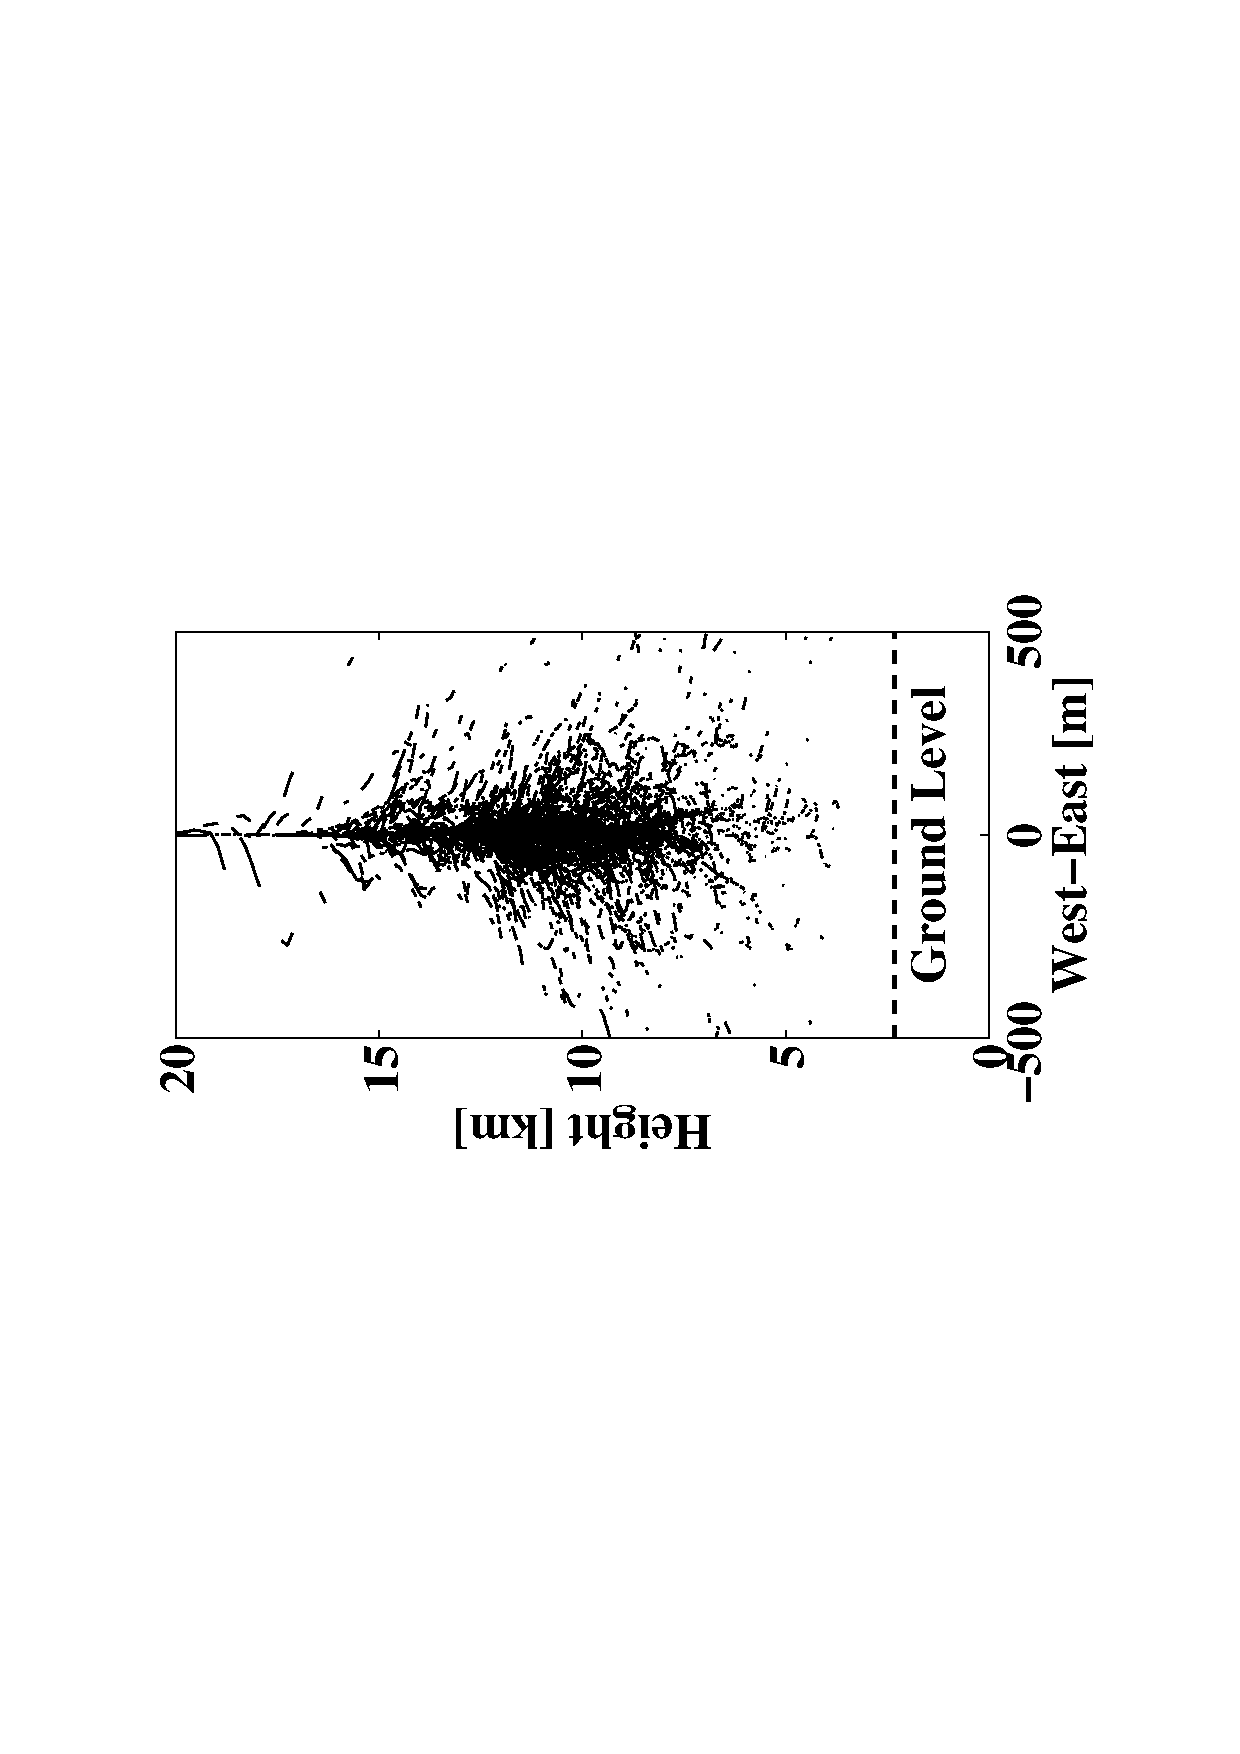
\includegraphics[draft=false]{plots/chap-technique/kas_gamm_100_tr.pdf}}}%
\resizebox*{!}{\textheight}{\rotatebox{270}{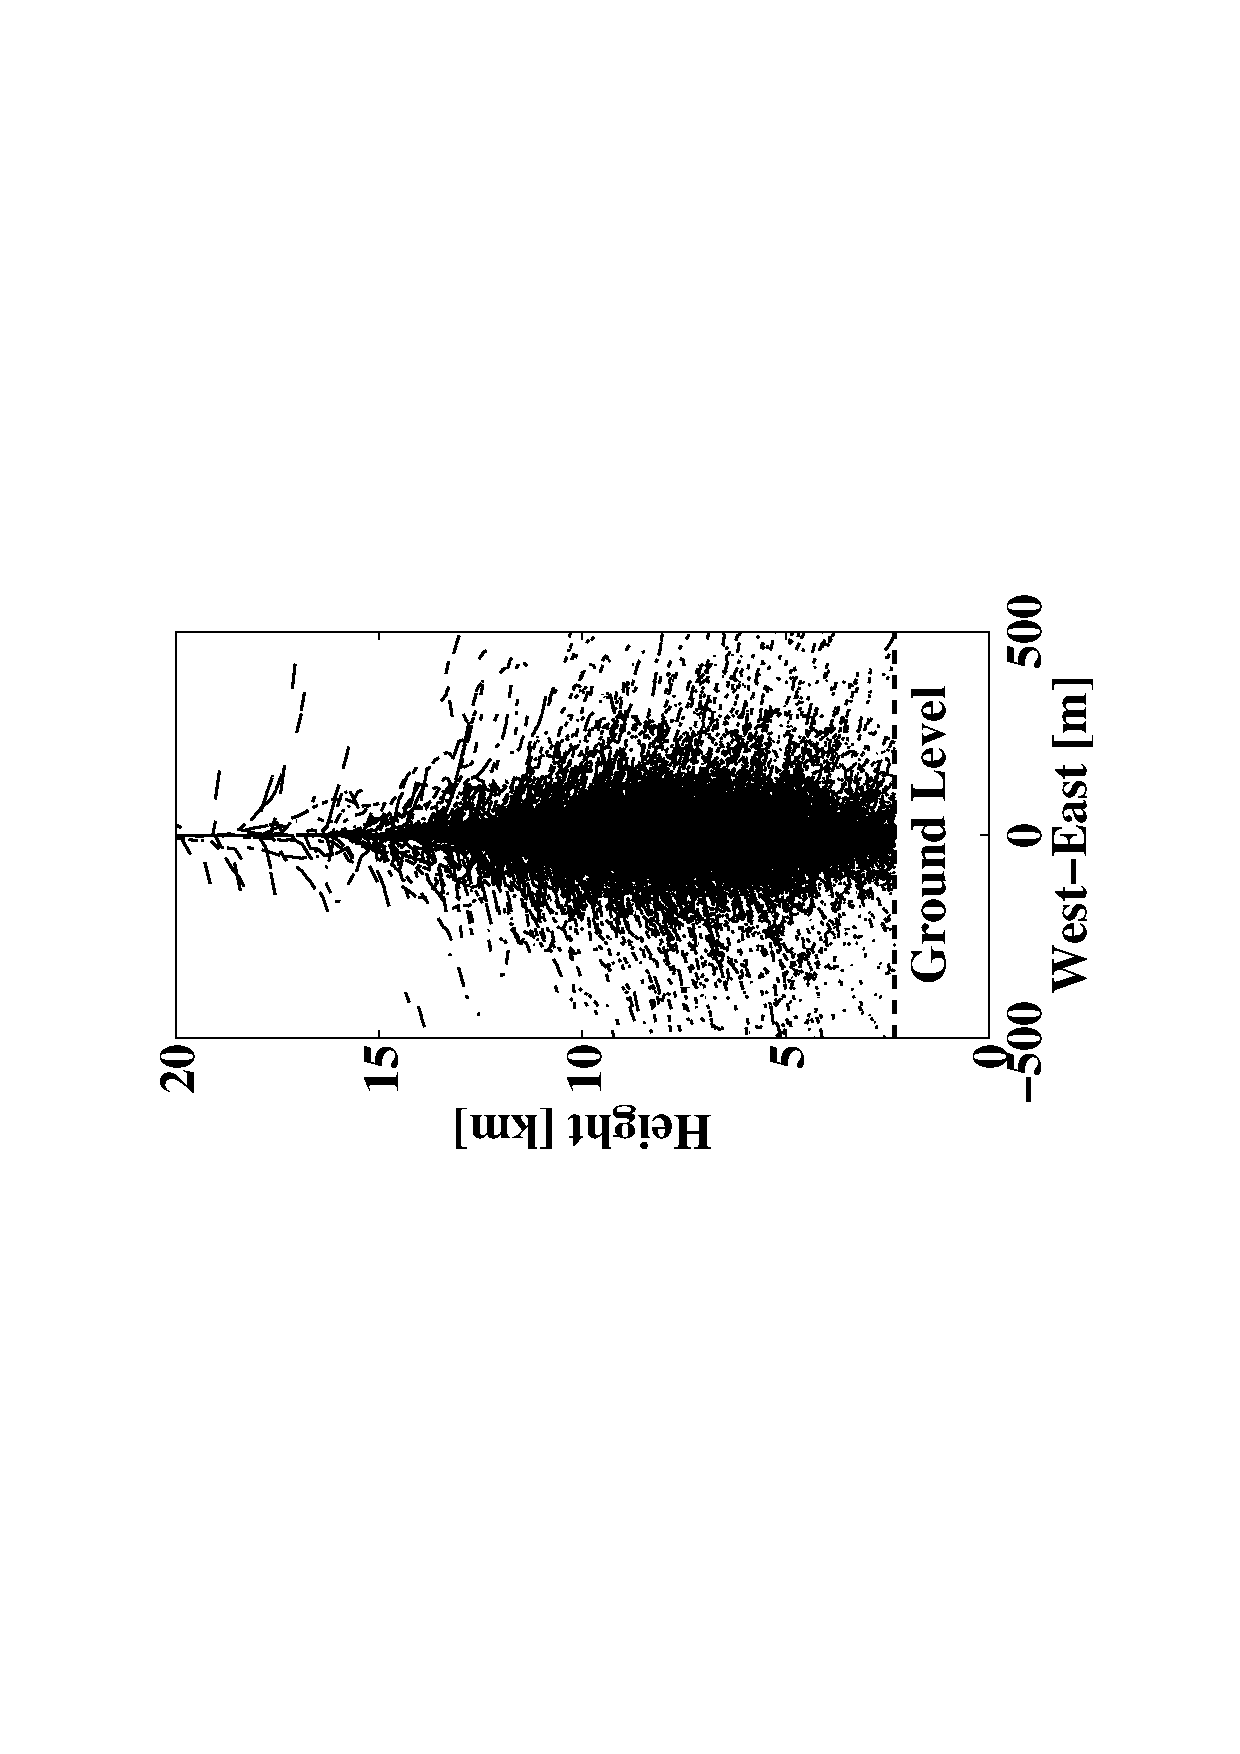
\includegraphics[draft=false]{plots/chap-technique/kas_gamm_1000_tr.pdf}}}%
\resizebox*{!}{\textheight}{\rotatebox{270}{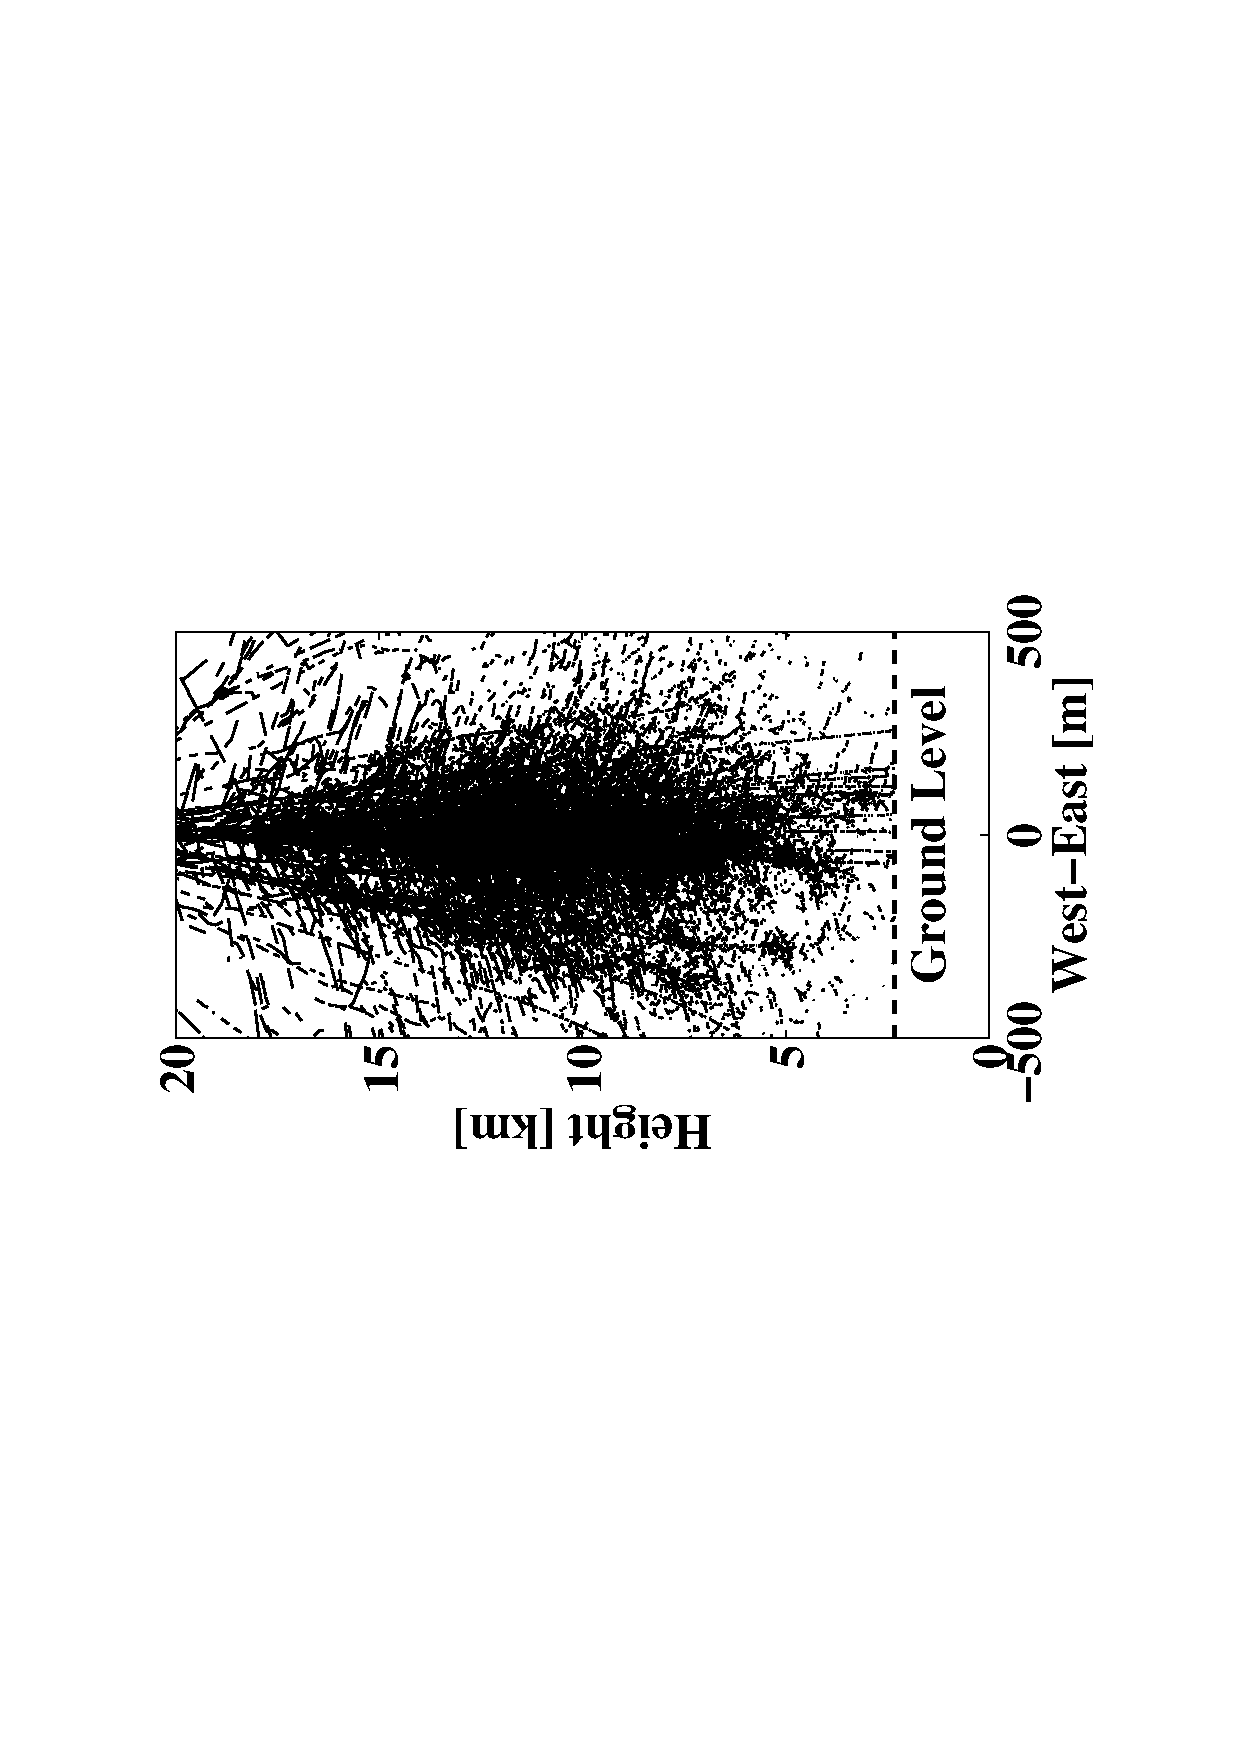
\includegraphics[draft=false]{plots/chap-technique/kas_prot_1000_tr.pdf}}}}}
\caption{\label{FIG::TECHNIQUE::SHOWERS} Simulated charged particle tracks 
in the atmosphere produced by a 100 GeV \Gray (left) and a 1\,TeV
\Gray (middle) and 1\,TeV proton (right). The horizontal and vertical
scales are not equal on this plot. Ground level is set for Mt. Hopkins
at 2320\,m A.S.L.}
\end{figure}

In addition to the electromagnetic component of E.A.S.\ discussed
above, showers initiated by cosmic-rays are dominated by a hadronic
component produced during the initial strong interactions in the upper
atmosphere. These interactions are violent and unpredictable but the
most important end products are neutral and charged pions which decay
to a pair of \Grays or a muon/muon-neutrino pair depending on the
charge of the pion. The
\Gray pairs result in electromagnetic cascades as described above. The
muons, which were identified as a mysterious ``penetrating radiation''
by early cosmic ray researchers, reach the ground with little further
interaction. Since muons take a considerable amount of the energy of
the primary, air-showers produced by hadronic primaries are typically
smaller than those produced by a \Gray of the same energy. Finally,
since the initial strong interactions tend to impart a larger
transverse momentum to the secondaries, a hadronic air-shower will
typically be broader than a \Gray induced shower, consisting of
overlapping cascades produced by different $\pi^0$ particles which
were initially had slightly different directions of propagation. 
Figure~\ref{FIG::TECHNIQUE::SHOWERS} illustrates the distribution of
charged particles in a shower produced by a 1\,TeV proton. Several
muons are visible as straight particle tracks reaching ground level.

\section{Imaging atmospheric \Cerenkov technique}
\label{SEC::TECHNIQUE::IACT}

A third component of all E.A.S.\ is \Cerenkov radiation
\citep{REF::JELLEY::BOOK1958}, produced as
the charged particles in the shower (e$^\pm$ and $\mu^\pm$) traverse
the atmosphere at speeds in excess of the speed of light in
air. \Cerenkov radiation was first noticed in the early 1900s by the
Curies but remained largely a mystery until the 1930s when it was
investigated in a series of experiments which exposed very pure
liquids to $\beta$-radiation \citep{REF::CERENKOV::1934}. The
phenomenon was later explained classically as the coherent
reinforcement of radiation emitted as the charged particle displaces
electrons in the dielectric medium through which it passes
\citep{REF::FRANKTAMM::1937}, work for which the three were awarded
Nobel prizes in 1958. In a tenuous gas medium such as air, where
$n\approx 1-\alpha\rho$ (with $\alpha<<1$) describes the weak
dependence of the index of refraction on the density of the medium,
the \Cerenkov threshold, characteristic angle and intensity of
radiated per unit length of the particle track
\citep{REF::JACKSON::CHAP13} may be written

\centerline{\begin{tabular}{rcll}
$E_t$ & $\propto$ & $\rho^{-1/2}$ & $100-20$\,MeV for e$^-$ between 
25km and sea-level\\
$\theta$ & $\propto$ & $\rho^{1/2}$ & $0.3-1.4^\circ$ \\
$I(\omega)$ & $\propto$ & $\rho$ & $2-30$ photon\,m$^{-1}$ \\
\end{tabular}}

The profile of \Cerenkov light emitted from a very energetic muon
traveling vertically through the atmosphere is illustrated in
figure~\ref{FIG::TECHNIQUE::CERENKOVMUON}. The effect of the changing
atmospheric density along the path of the muon and the resultant
change in the \Cerenkov emission angle causes a focusing of the
\Cerenkov light on the ground and an enhancement of the photon density
at distances of $\sim$120\,m from the muon impact location on the
ground. The photons that strike the ground at distances of $<$30\,m
are due to emission from the region of the atmosphere close to ground
level. The photon density in this region tends to infinity as 1/r
reflecting the essentially constant emission intensity close to the
ground level. Since the atmosphere is a strong absorber of light in
the U.V. region, such ``local'' photons tend to have a spectrum with an
enhanced U.V. component with respect to emission from higher in the
atmosphere. The power of the atmospheric \Cerenkov technique is that a
sufficiently large and sensitive detector can be placed anywhere in
the 45,000\,m$^2$ light pool to detect the particle.

\begin{figure}[t]
\resizebox{\textwidth}{!}{\resizebox*{!}{\textheight}{\rotatebox{270}{\includegraphics{plots/chap-technique/cones.pdf}}}%
\resizebox*{!}{\textheight}{\rotatebox{270}{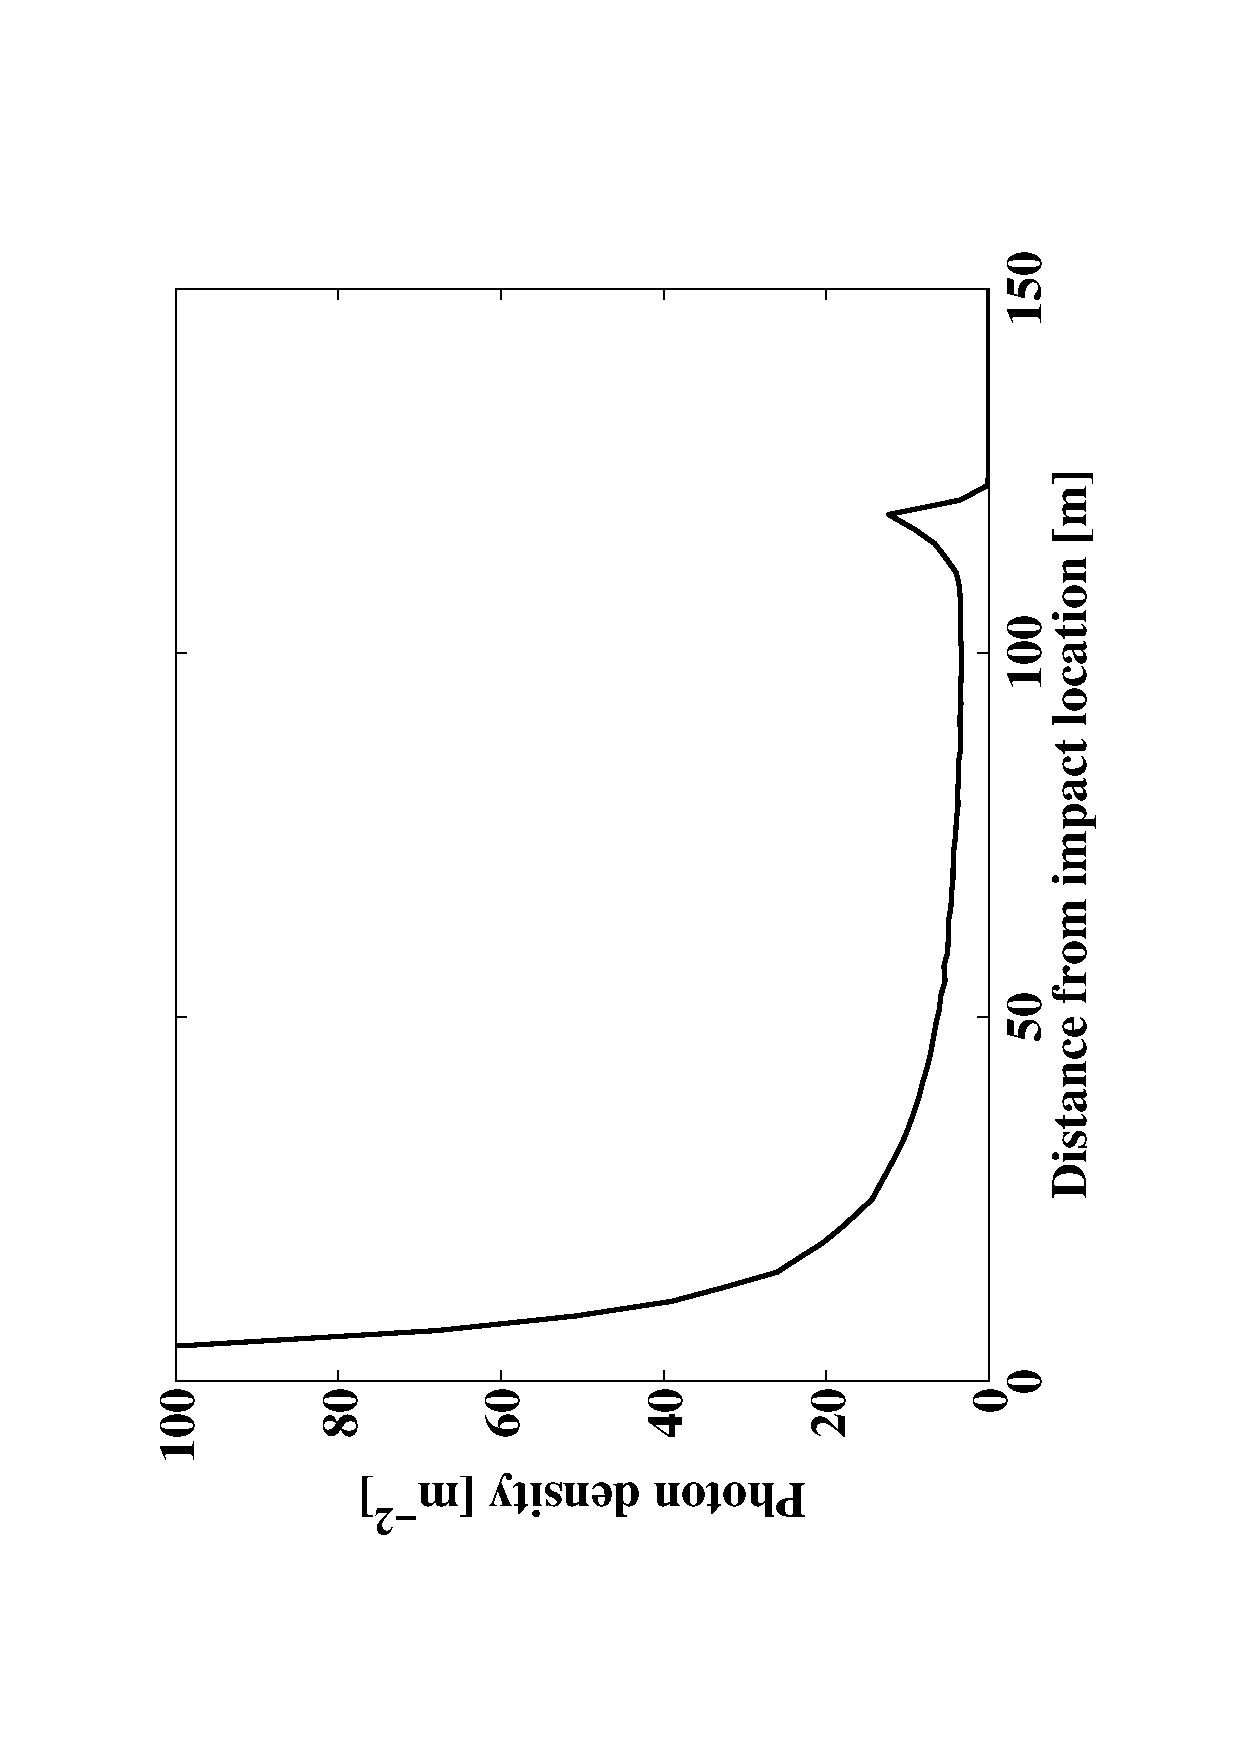
\includegraphics{plots/chap-technique/kas_muon_99999_rd.pdf}}}}
\caption{\label{FIG::TECHNIQUE::CERENKOVMUON} Left: Illustration of 
\Cerenkov emission from vertically moving muon. Right: Radial density 
on the ground of \Cerenkov photons with 200\,nm$<\lambda<$700\,nm,
showing enhancement at 120\,m due to focusing effect of the
increasing atmospheric density. Since the intensity of emitted photons
is essentially constant as the muon reaches the ground, the radial
density diverges like 1/r, as r$\rightarrow$0. }
\end{figure}

The profile of \Cerenkov light from purely electromagnetic air showers
has features similar to the single particle light profile described
above. In general, the transverse momentum (with respect to the
original primary) imparted to the shower particles is small and the
\Cerenkov light pool covers approximately the same area as above.  The
enhancement at 120\,m is also prominent since a considerable amount of
emission comes from the $10-15$\,km region of the atmosphere (see
figure~\ref{FIG::TECHNIQUE::CERENKOVMUON}). At distances greater than
120\,m from the shower core, the fall-off in \Cerenkov density is
slower than single particle case due to multiple Coulomb scattering in
the shower. The \Cerenkov density typically increases with the energy
of the primary as the number of charged particles in the shower core
increases and the development of the shower occurs deeper into the
atmosphere where the density is higher. In addition, the locally
generated \Cerenkov component becomes more significant for larger
showers; a typical 100\,GeV shower, which does not extend to ground
level, will have no local light.

The distribution of \Cerenkov light from hadronically induced showers
is quite different from the electromagnetically induced case above. In
general, a number of muons will be present in the shower which give
rise to considerable local light distributed around their ground
impact locations. Additionally, hadronic showers usually have a number
of EM cascades resulting from decay of different $\pi^0$ particles
which can have considerable transverse momenta. The \Cerenkov light
produced by these photons gives rise to clumps in the distribution on
the ground. In some small fraction of cases most of the energy of the
primary can go to a single $\pi^0$ and an essentially electromagnetic
shower can arise with properties almost identical to {\Grayc}-induced
showers. Finally, in the hadronic case, there tends to be a large
variance in the profile of showers triggered by identical primaries,
due to the initial strong force interactions.

The detection of \Cerenkov light from air-showers was pioneered by
\citet{REF::GALBRAITHJELLEY::1953, REF::GALBRAITHJELLEY::1955} using a
ten inch mirror with photomultiplier tube at its focus. Since these
early experiments, the desire to discriminate {\Grayc}-induced
air-showers from the overwhelming background of hadronic showers has
largely driven the design of atmospheric \Cerenkov instruments. The
development of the imaging technique by the Whipple collaboration
yielded the first detection of very high energy \Gray emission from an
astronomical source \citep{REF::WEEKES::APJ1989}. The essence of the
imaging technique is to take a snapshot of the \Cerenkov flash
associated with the air-shower using a high resolution camera system
consisting of an array of close packed photo-tubes mounted at the focus
of a large telescope, fast triggering and readout electronics to
digitize the $\sim$10\,ns signals and a data acquisition system capable
of recording the data with a minimum of dead time. 

\begin{figure}[t]
\centerline{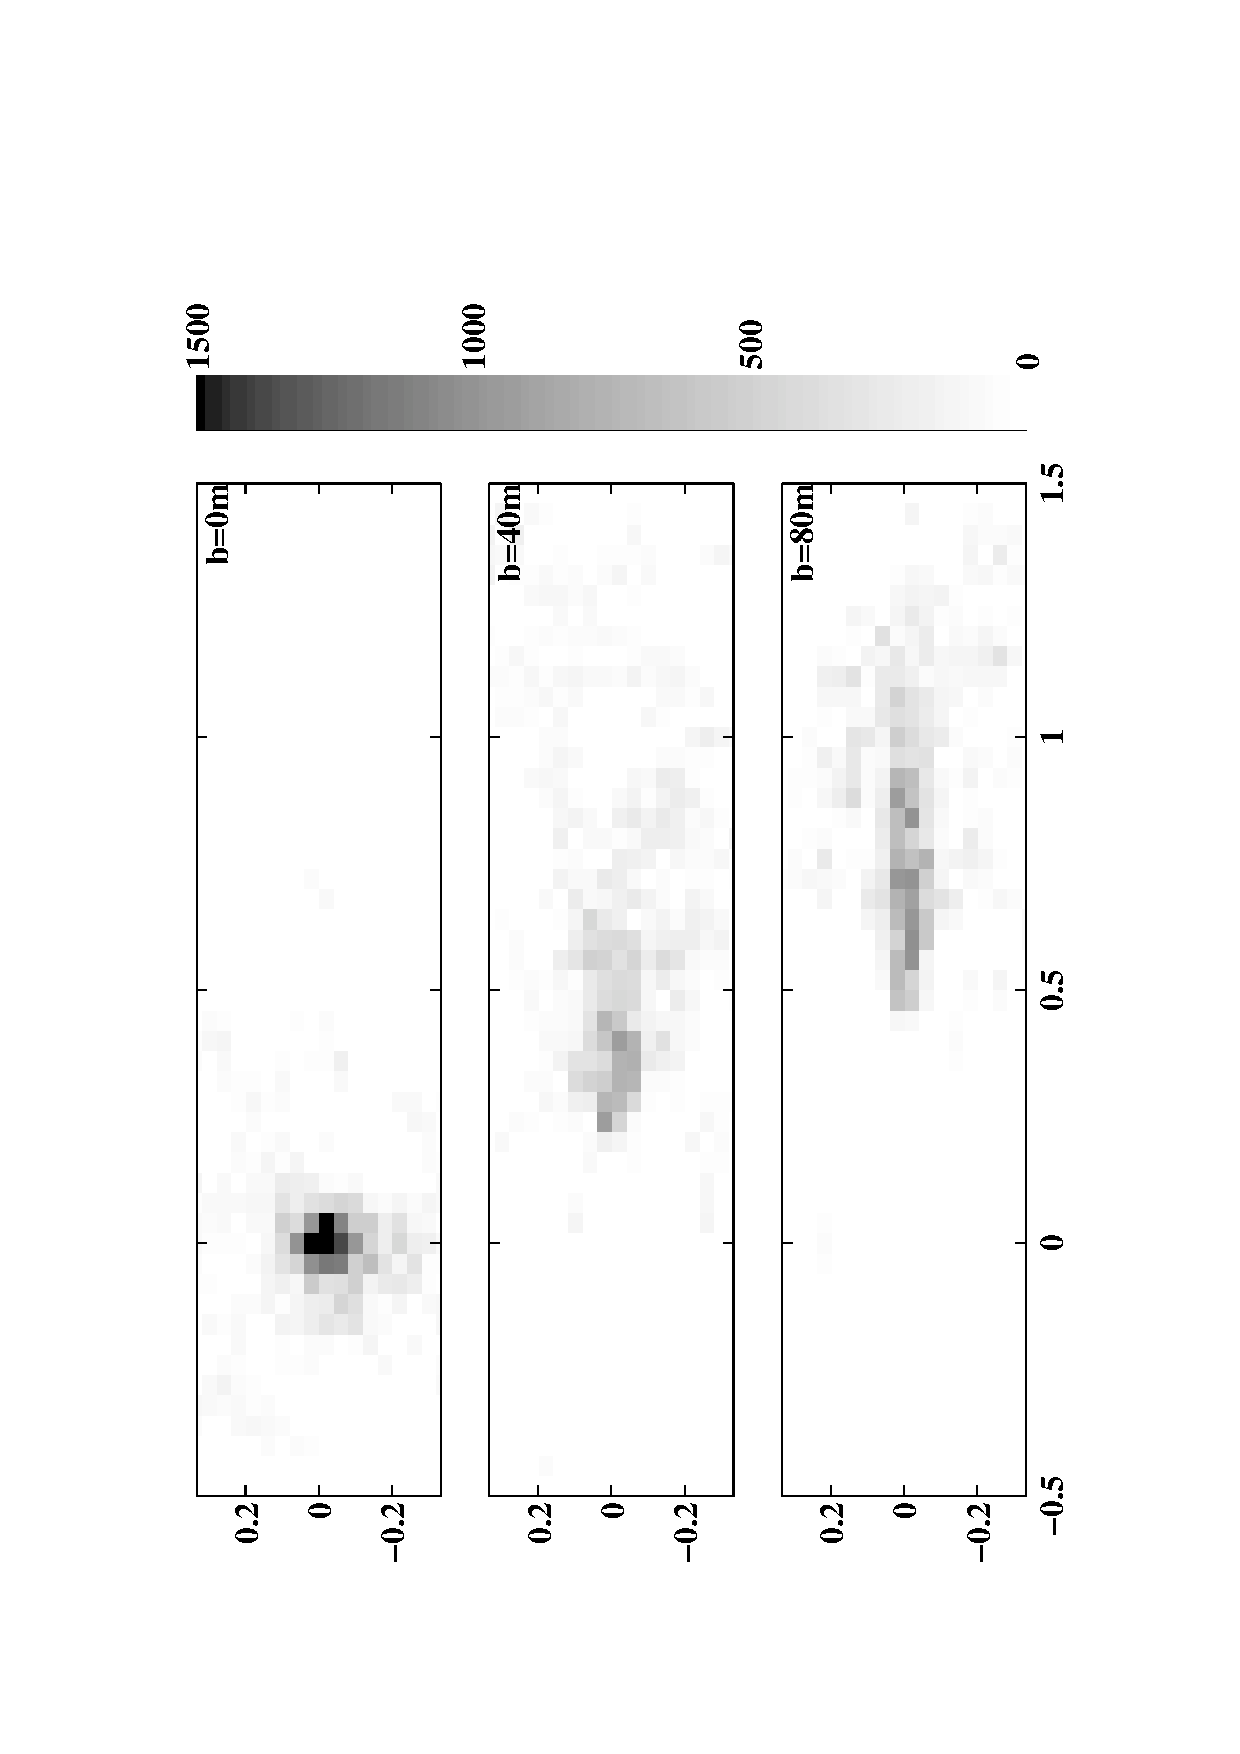
\includegraphics[angle=270,width=0.65\textwidth]{plots/chap-technique/fplane_density.pdf}}
\caption{\label{FIG::TECHNIQUE::FPDENSITY} Density of photons per 
unit mirror area in the focal plane of an ideal 10\,m telescope for a
simulated 350\,GeV photon induced shower, in units of
m$^{-2}$\,deg$^{-2}$. The same shower is shown for three different
impact parameters: 0\,m, 40\,m and 80\,m. The axes gives the angular
distance in the focal plane from the direction of the primary (which
is assumed to be coincident with the center of the camera) in
degrees.}
%The shading scale does not fully
%accomodate the density of the brightest bins in the $b=0$ image, which
%contains considerable local light.}
\end{figure}

In the focal plane of such an instrument, the image traces the
development of the shower in the sky. For an EM induced shower the
image is largely symmetric around the projection of the shower axis
onto the field of view of the instrument, reflecting the symmetry of
the shower itself around the axis. The images of EM showers are often
described as ``cometary''; one side of the shower, in the direction of
towards the early stages of the shower development (i.e.\ towards the
upper atmosphere) has a higher photon density. As the shower dies
after shower maximum, the image becomes more diffuse with a lower
photon density, spread out over a larger area of the image.  Higher
energy showers produce more secondaries, more \Cerenkov photons and
extend further into the atmosphere, resulting in an image which has a
larger photon density and a larger extent in the field of view.
Finally the appearance of the shower in the field of view is dependent
to a large extent on the distance between the shower axis and the
instrument, usually called the \textit{impact parameter} and denoted
as $b$. Figure~\ref{FIG::TECHNIQUE::FPDENSITY} illustrates an image of
a 350\,GeV \Gray shower viewed at three different impact parameters.
The showers become elongated and displaced from the center of the
camera as the impact parameter increases. Images of proton induced
showers are less compact than \Gray showers, due largely to the higher
transverse momentum imparted by the strong interactions. Data
selection criteria, based on these differences, capable of keeping a
large fraction of the \Gray events while discarding the majority of
the background cosmic-ray events are described in
chapter~\ref{CHAP::ANALYSIS}.

\section{Trigger and acquisition electronics}
\label{SEC::TECHNIQUE::ELECTRONICS}

\begin{figure}[p]
\centerline{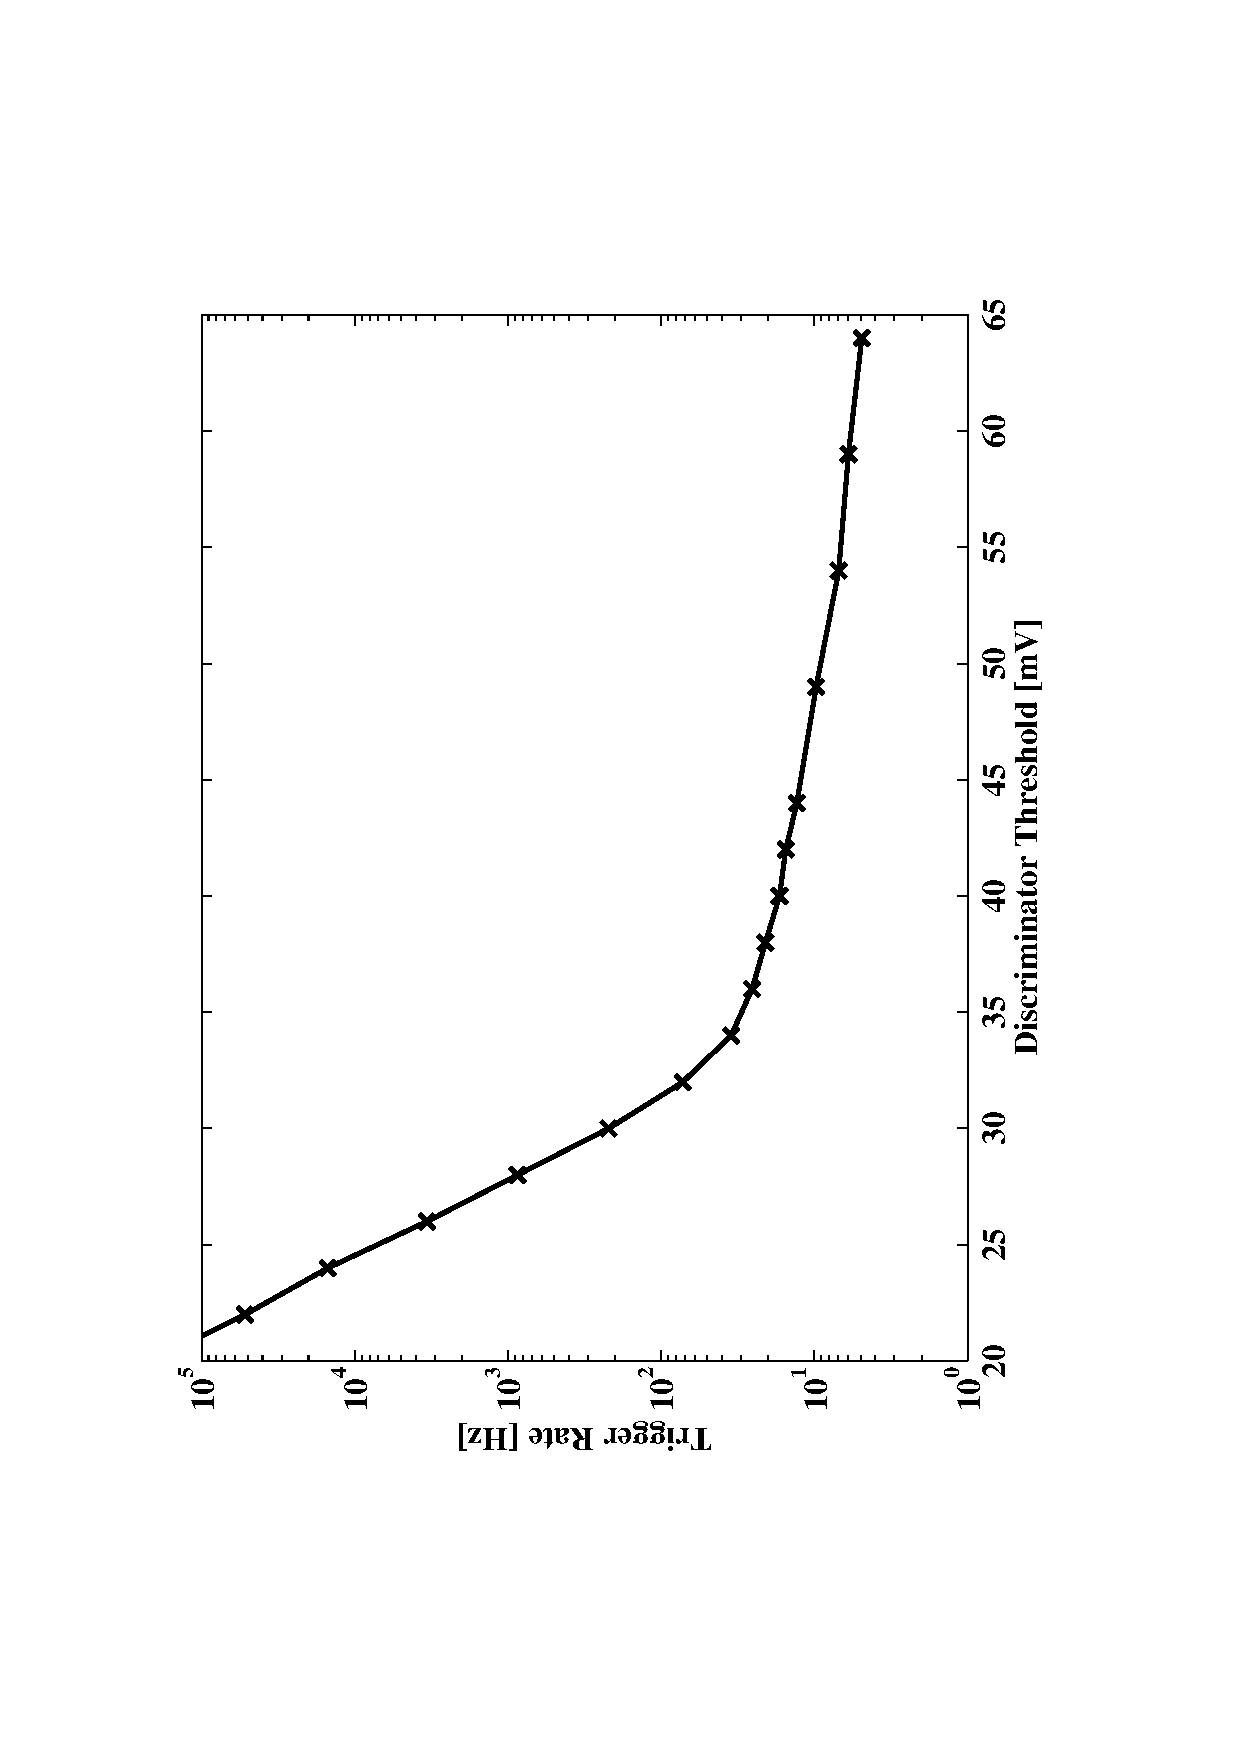
\includegraphics[angle=270,width=0.7\textwidth]{plots/chap-technique/bias_011009.pdf}}
\caption{\label{FIG::TECHNIQUE::BIASCURVE} Event rate vs.\ L-1
trigger threshold with a trigger L-2 requirement (pattern selection
trigger) of three adjacent channels exceeding the threshold within the
coincidence time. This kind of plot is usually referred to as a ``bias
curve''.}
\end{figure}

\begin{figure}[p]
\centerline{\includegraphics[width=0.7\textwidth]{plots/chap-technique/el_schematic.pdf}}
\caption{\label{FIG::TECHNIQUE::ELSCHEMATIC} Schematic of the major
components of the data acquisition system. See text for discussion.}
\end{figure}

Readout of the 379 channel camera is initiated by a two-level trigger
system. At the lowest level (L-1), each of the inner 331 channels are
monitored by a constant fraction discriminator (CFD), which triggers
when the signal exceeds a pre-programmed level. For a constant pulse
profile, the CFD compensates for the time jitter intrinsic to a
standard discriminator (i.e.\ simple voltage comparator), which
triggers earlier, relative to the peak in the pulse profile, for
signals with large amplitude. The digital outputs of these CFDs are
then processed by the second level of trigger (L-2), an electronic
system referred to as the \textit{pattern selection trigger} or
PST\footnote{Actually, there are two separate electronic systems
involved in the L-2 trigger. The second system, called the
multiplicity trigger, has very little time jitter in comparison to the
PST, and is used only to set the timing of the L-2 output.}, which is
essentially a memory lookup table that can be programmed to
discriminate images with two, three or four adjacent channels from
those where the triggering channels are non-adjacent. This trigger
design, which preferentially records images of compact \Gray and
hadronic showers over the random fluctuations of the night-sky
background, is described in detail in
\citet{REF::BRADBURY::1999SLC}. In general it is desirable to set the
discriminator threshold as low as possible, allowing lower energy
events to be recorded. At low trigger levels, the night-sky background
light causes an excessive event rate, even with the PST. The trigger
is set to ensure that the event rate is below the maximum sustainable
rate of the data acquisition system, $\sim35$\,Hz, even when observing
the brightest fields of view. Figure~\ref{FIG::TECHNIQUE::BIASCURVE}
shows the trigger rate vs.\ trigger threshold, as measured in late
2001. At high thresholds, the rate is dominated by the power-law
cosmic-ray spectrum; below approximately 35\,mV the rate curve becomes
very steep, due to random triggers by night-sky noise. A setting of
$\sim38$\,Hz would result in a relatively stable rate, even under the
brightest of conditions.

A schematic of the main components of the data acquisition system is
shown in figure~\ref{FIG::TECHNIQUE::ELSCHEMATIC}. The signal from
each channel, after $\times10$ amplification, is digitized by a set of
LeCroy 2249A 0.25\,pC/count charge-to-digital converters (QADC).
Conversion is initiated by the L2 trigger; in order to allow for the
trigger decision to be formed, the signals are delayed in a length of
RG-58 cable, allowing the trigger decision and signals from the PMTs
to reach the ADCs coincidentally. The integration time of $\sim$20\,ns
is longer than the intrinsic duration of the \Cerenkov flash on the
ground, in order to account for the time-spread introduced by the
spherical mirror (see figure~\ref{FIG::INTRODUCTION::SCOPE}) and
dispersion in the delay cables. As a consequence, more night-sky noise
is integrated in the signal that would otherwise be the case. Future
experiments will minimize this noise by having mirrors with longer
focal lengths (hence smaller time-spreads) and by eliminating the need
for long signal delay cables using electronic delay systems. One
approach to the latter is to continually sample the signal with flash
ADCs, storing the digitized information in a temporary RAM buffer
which can then be read out when the trigger decision is made.

The signal is AC coupled at the input of the amplifier to remove any
bias current through the tube, due mainly to the night-sky brightness
that the tube is exposed to in addition to the (significantly smaller)
dark current in the tube. A small biasing, or pedestal, current is
then reintroduced to the signal in the input stage of the QADCs to
facilitate the measurement of negative fluctuations of the signal from
the mean sky-brightness. This biasing current is removed during the
analysis of the data, as described in
section~\ref{SUBSEC::ANALYSIS::PEDESTAL}. The data is read out over a
computer network and stored on disk for offline analysis.

It is estimated that a single photo-electron in the PMTs produces a
signal of $\sim3.3$\,counts in the QADC. This corresponds to a total
gain in the system of $\sim5\times10^{6}$.

\section{Characterization of detector}
\label{SEC::TECHNIQUE::CHARACTERISTICS}

Unlike the lower energy satellite based \Gray instruments, the
response of a ground-based \Cerenkov telescopes cannot be measured
using an artificial test beam. Characterization of the response of
such instruments to \Grays and cosmic-rays must be done using
simulations, by modeling the air-shower development, \Cerenkov light
production and detector response. For such a study to be accurate, the
simulations must correctly account for such factors as: nuclear
physics cross-sections (especially for hadronic simulations),
atmospheric density profile and response to \Cerenkov radiation,
wavelength dependent mirror reflectivity and PMT quantum efficiency,
dispersion in the cables, response of the trigger and ADCs, and
others. Many of these can be accurately measured in the laboratory,
others must be extrapolated from standard tables, such as the U.S.\
standard atmosphere model. It is estimated that the accuracy of such a
simulation study $\sim20$\%. This is borne out by the impressive
agreement in the spectrum of the Crab Nebula source calculated, from
observations, by the various ground-based VHE observatories in the
northern hemisphere, such as Whipple, HEGRA and CAT. These groups
employ different simulation codes, both for shower physics and
detector simulation, yet derive spectra for the Crab that agree to
within the limits of statistical and systematic errors.

Chapter~\ref{CHAP::VERITAS} describes the study of a next generation
ground-based instrument, VERITAS, in some detail. The results of a
similar study of the Whipple telescope are presented here, with a
brief description of the simulations.

The KASCADE simulation package \citep{REF::KERTZMAN::1994NIMA} was used
to generate sets of {\Grayc}-induced air shower events. Sets of
{\Gray}-induced events were generated over a range of energies between
30\,GeV and 30\,TeV. The energy bins were evenly distributed in $\log
E$ with eight bins per decade of energy. To accommodate the decreasing
detection efficiency of the instrument at lower energies, the number
of events simulated per bin was chosen to increase sharply at lower
energies, to ensure that sufficient events were available so that some
of them would survive the simulated trigger requirements and data
selection procedure.

For each event, the \Cerenkov photons generated in the shower were
traced to see whether they intersected the mirror. The wavelength
dependent reflectivity was accounted for and, if the photon was
reflected into a PMT, so also was the quantum efficiency of the tube.
The resultant photo-electrons produced by the shower (if there were
any) were combined with artificially generated, Poisson distributed,
night-sky photo-electrons, producing a realistic image that is
comparable to an image of a real \Grayc. The images were subjected to
the standard trigger requirement of three neighboring channels above a
threshold of $\sim7$ photo-electrons. Those events that pass the
trigger requirement are then processed using the standard analysis and
data selection criteria, as described in chapter~\ref{CHAP::ANALYSIS}.
Figure~\ref{FIG::TECHNIQUE::AREA_DRDE} shows the simulated response of
the instrument to on-axis \Gray primaries at an angle of $20^\circ$
to the zenith. For a Crab Nebula like spectrum (power law --
$dF/dE\propto E^{-2.5}$) the instrument is most sensitive to \Grays
with energy of $\sim$350\,GeV. It is usual to refer to this as the
\textit{peak response energy} of the instrument\footnote{Or somewhat
incorrectly, as the \textit{energy threshold} of the instrument.} and
to quote fluxes and upper-limits measured with the instrument at that
energy.

\begin{figure}[t]
\centerline{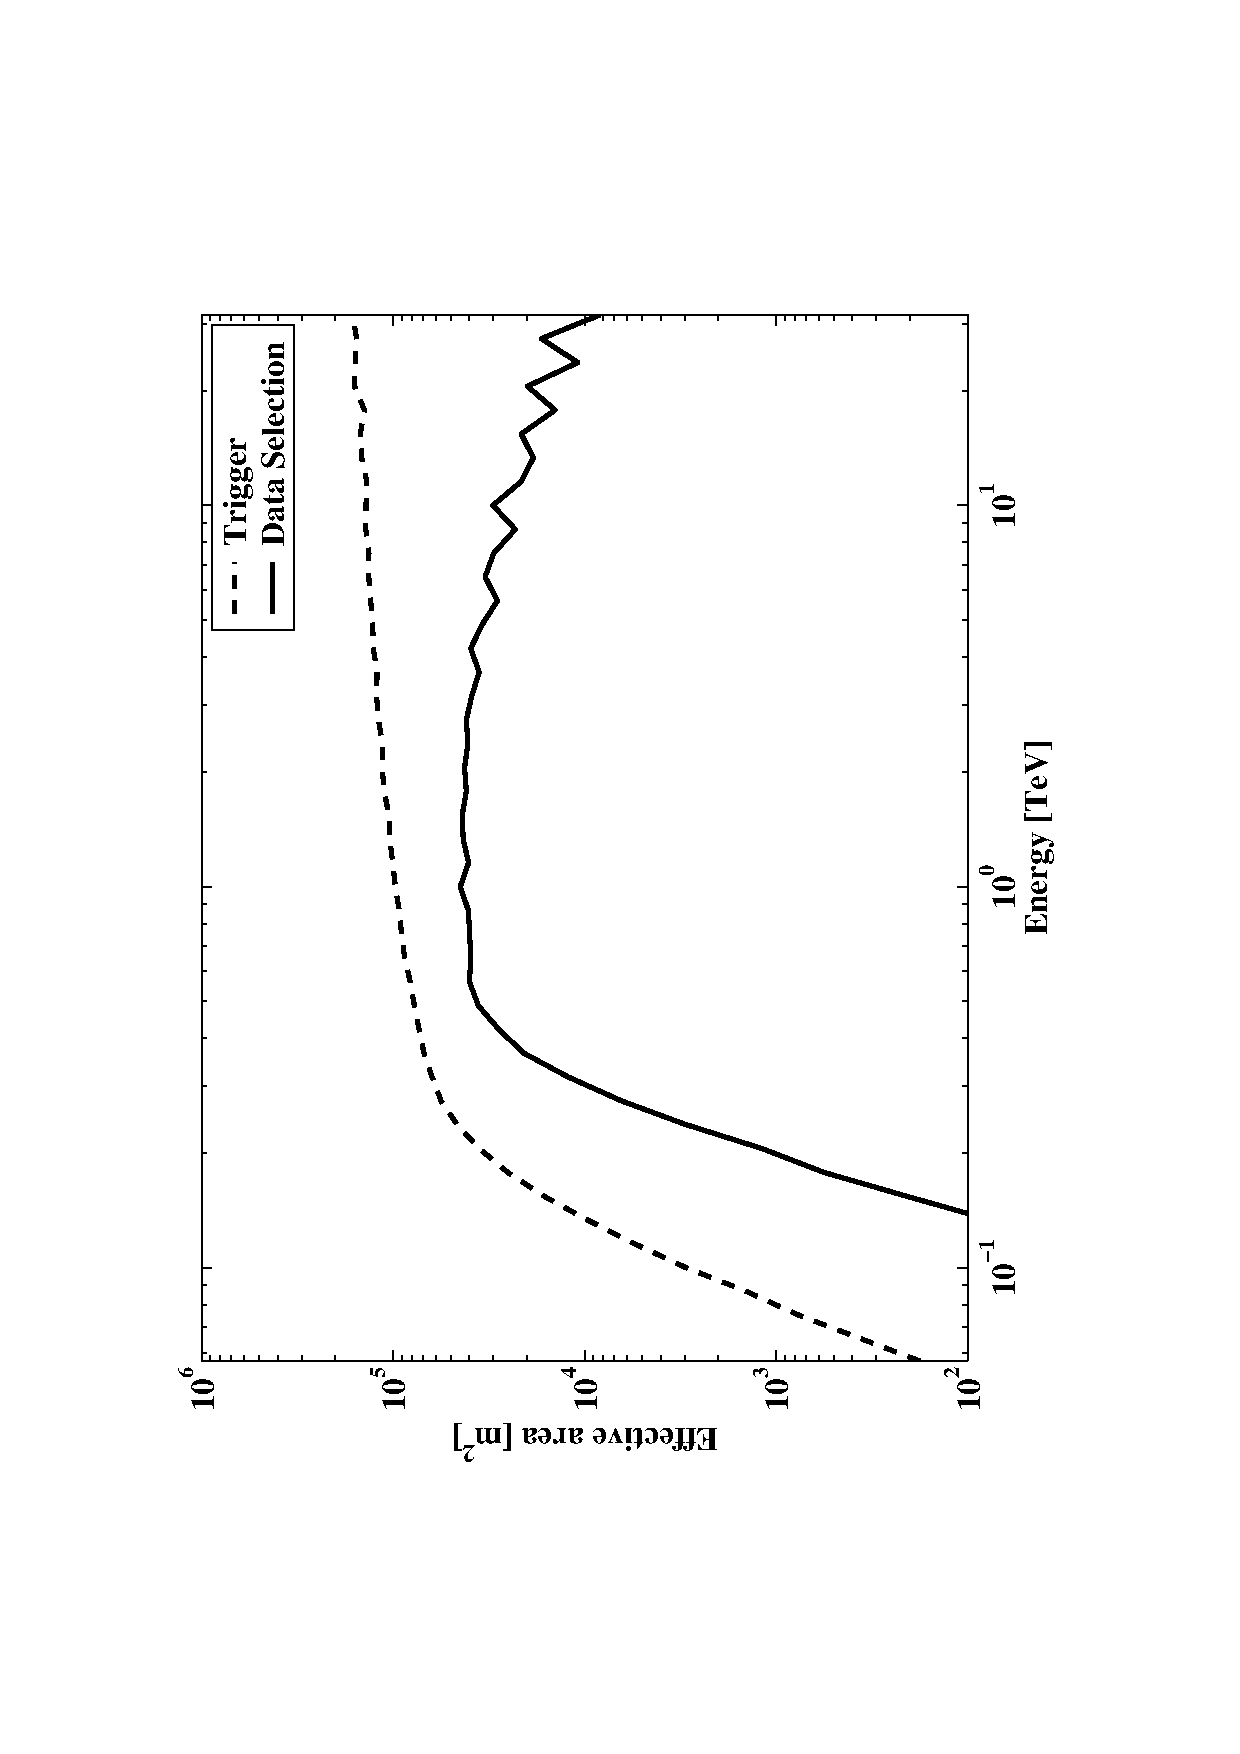
\includegraphics[angle=270,width=0.49\textwidth]{plots/chap-technique/detector_response_area.pdf}\includegraphics[angle=270,width=0.49\textwidth]{plots/chap-technique/detector_response_drde.pdf}}
\caption{\label{FIG::TECHNIQUE::AREA_DRDE} (Left) Effective
collection area vs.\ energy for trigger and for data selection
algorithm. After data selection, the collection area peaks at
$\sim4\times10^4$\,m$^2$. (Right) Differential rate of \Grays
collection from Crab Nebula. } \end{figure}


\chapter{Data Analysis}
\label{CHAP::ANALYSIS}
\newcommand{\Pairs}{\textsc{On/Off}}

A number of data analysis algorithms have been developed by the VHE
\Gray community, some of which are specialized for different classes 
of instrument or to different classes of candidate \Gray source. One
of the simplest, most effective, single telescope, point-source
analysis techniques, dubbed ``Supercuts'', was developed for data
taken at the Whipple 10\,m telescope \citep{REF::PUNCH::NATURE1992}. 
Data selection is based on a set of strict cuts applied to a set of
parameters which are calculated for each image. The selection cuts are
optimized to preferentially select \Grayc-induced events over
background events. This technique typically keeps 50\% of \Gray events
and discards $>$99\% of background events, significantly improving the
signal-to-noise (S/N) ratio. For a bright source such as the Crab
Nebula, a S/N ratio corresponding to a $>$4$\sigma$ rejection of the
null hypothesis that no source is present (with an event rate large
enough that Gaussian statistics apply) can be achieved in 30 minutes
of observations. This point-source analysis technique has been adapted
to sources whose location is not well defined, and to extended sources
by \citet{REF::LESSARD::2001APP}. A refinement of this technique is
presented here.

\section{Observations}
\label{SEC::ANALYSIS::OBSERVATIONS}

To avoid damage to the photo-multiplier tubes, observations with the
Whipple 10\,m telescope are made only during the portion of the night
during which the moon is below the horizon. Observations are thus
restricted to $\sim3$\,week periods, called ``dark runs'', separated
by the period of the full moon. The telescope does not operate during
the two month summer monsoon season to protect the sensitive
electronics from the frequent lightning strikes on the mountain. The
close-down period is used to perform maintenance upgrades to the
instrument; hence, its characteristics usually change during this
summer period. Observations are divided, therefore, into ten month
``observing seasons'' when the characteristics of the instrument
remain largely constant. Data for this survey was taken from 1999 to
2003. Significant changes were made to the instrument during the
summer and fall of 2001 when a new approach to the alignment of mirror
facets was implemented. This new technique corrected for the
deformations in the optical support structure which occur as the
telescope is elevated from its stow position
\citep{REF::SCHROEDTER::2002APS}.

Observations with the instrument are made in one of two modes, termed
\Pairs\ and \Trk\ modes, which have significantly different approaches
to background estimation. When operating in the \Pairs\ mode, two
separate 28\,minute scans (\On\ and \Off) are made. The \On\ scan is
taken while tracking the sky with the candidate object at the center
of the field of view and gives an estimate of the \Gray flux combined
with the background rate. The \Off\ scan is taken in the absence of
the candidate object to give an independent estimate of the background
rate. The \On\ and \Off\ scans are taken such that they are separated
by 30\,minutes in time and track locations in the sky separated by
30\,minutes in Right Ascension. Thus, the scans cover the same range
of elevation and azimuth, which helps to minimize differences in the
background rate between each scan. In general, \Pairs\ mode is only
used in the best weather conditions as large differences in the
background rate between the two scans are introduced if any cloud
drifts through the field of view. \Pairs\ mode can be used to test the
hypothesis that \Gray emission is occurring from any location within
the field of view of the instrument. This is the case for a candidate
source whose location is not known a priori, such as unidentified
sources with large error-box locations and for sources whose emission
is expected to be extended, such as SNR.

When operating in the \Trk\ mode, a single scan is taken tracking the
candidate object. An estimate of the background is inferred from the
number of events present in the scan which are not consistent with
having originated from the candidate source location. The ratio of
background events which are consistent with having originated from the
source to those which are not, must be calculated independently using
data which are known not to have a source present, a process described
in section~\ref{SEC::ANALYSIS::TRACKING}. \Trk\ mode is most
applicable when testing the hypothesis that \Gray emission is
occurring from a point-like object at the center of the field of view,
for example, when testing for emission from an extragalactic source or
pulsar whose location is well known. Since the background estimate is
derived from the observations themselves, twice the amount of
on-source data can be collected in a given time than can be collected
in \Pairs\ mode. The method implicitly assumes that the ratio of
events consistent with a candidate source to those which are not is
constant across the fields of all potential sources. This may not be
the case for fields with bright stars present for observations made
over a large range of elevations.

\section{Image Conditioning}
\label{SEC::ANALYSIS::CONDITIONING}

Prior to parameterizing the recorded images, five stages of image
conditioning are applied, with the aim of minimizing systematic
differences across the camera and between the \On\ and \Off\ scans,
and also to minimize the influence of background night-sky light on
the parametrization of the
images. Figure~\ref{FIG::ANALYSIS::CONDITIONING} depicts a typical
event after each stage of the image conditioning.

\begin{figure}[p]
\centerline{\resizebox{\textwidth}{!}{\resizebox*{!}{\textheight}{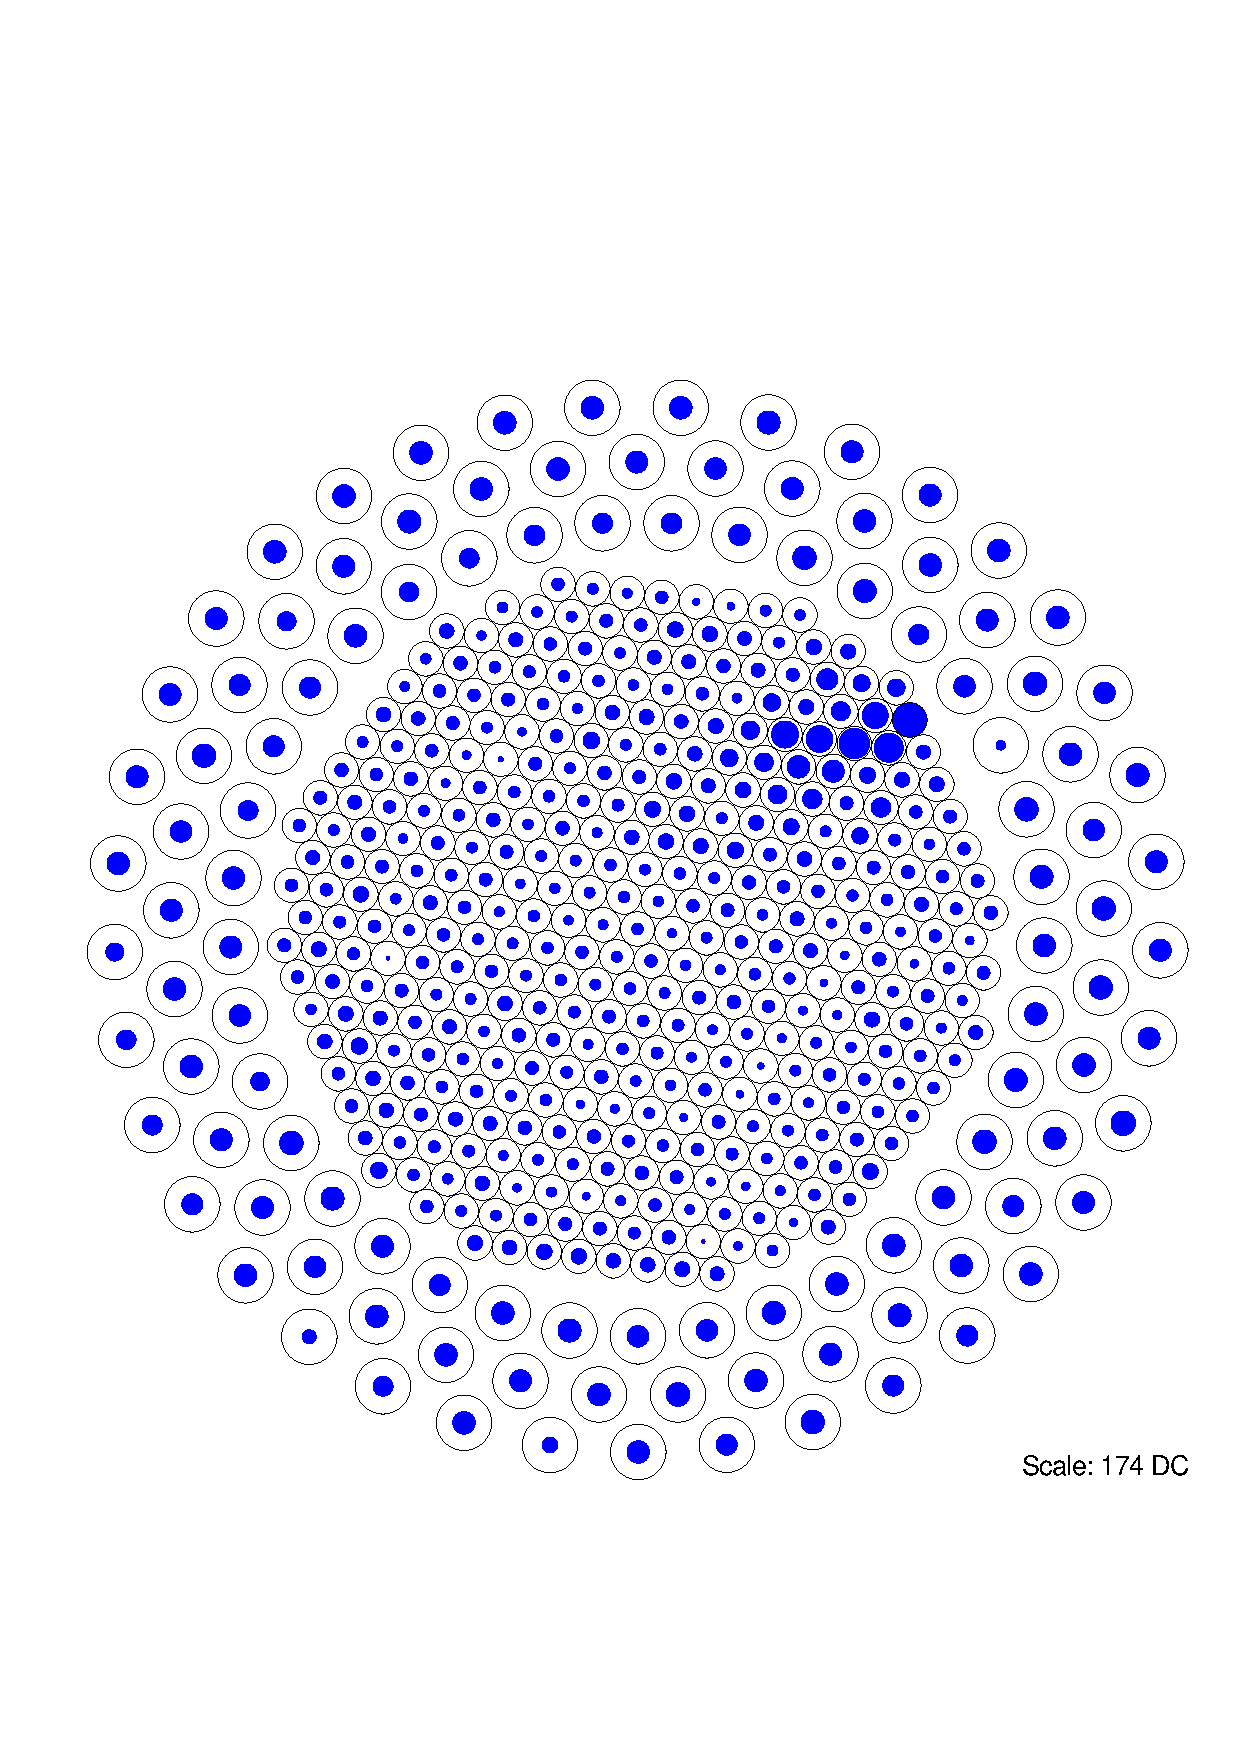
\includegraphics[draft=false]{plots/chap-analysis/gt023886_ev2652_raw.pdf}}%
\resizebox*{!}{\textheight}{\includegraphics[draft=false]{plots/chap-analysis/gt023886_ev2652_ped.pdf}}}}

\centerline{\resizebox{\textwidth}{!}{\resizebox*{!}{\textheight}{\includegraphics[draft=false]{plots/chap-analysis/gt023886_ev2652_gain.pdf}}%
\resizebox*{!}{\textheight}{\includegraphics[draft=false]{plots/chap-analysis/gt023886_ev2652_clean.pdf}}}}
\caption{\label{FIG::ANALYSIS::CONDITIONING} A typical event 
after each stage of image conditioning. (Top left) Raw ADC values. (Top
right) After subtraction of injected pedestals. (Bottom Left) After
gain equalization. (Bottom right) After cleaning.}
\end{figure}

\subsection{Pedestal Removal}
\label{SUBSEC::ANALYSIS::PEDESTAL}

The signal chain between the photo-tubes and ADCs is AC coupled at
the amplifier to remove any steady current associated with the
night-sky background and with any dark currents present in the PMT. To
allow negative fluctuations from the mean night-sky background to be
measured, a small biasing current is artificially injected into the
ADCs in order to yield a positive output for the largest reasonable
negative fluctuation, integrated over the 20\,ns ADC gate. This small
biasing current, dubbed the ``pedestal'', is set large enough to
accommodate a 4-5$\sigma$ negative fluctuation (with a typical, dark
sky, night-sky background rate) by adjusting a trim-potentiometer on
the ADC board. Typically the RMS fluctuations due to the night-sky
background are $\sim4-5$ digital counts (DC) when integrated by the
ADCs, so a bias current giving an integrated signal of $\sim20-25$\,DC
is chosen. The pedestal currents must be subtracted from the ADC
signals during the analysis to result in a mean of zero for each
channel when no signal is present.

In addition to the normal triggering requirement described in
section~\ref{SEC::TECHNIQUE::ELECTRONICS}, an artificial trigger is
generated from the 1\,Hz signal of the master GPS clock. This causes
events, which are flagged as special ``pedestal events'' in the data
stream, to be recorded in the absence of an air-shower. These events
record the zero-level point of each ADC in the presence of any
night-sky background and the injected pedestal current.

To estimate the level of the integrated pedestal current present in
each channel, these events are accumulated over the course of
observations (typically 1600 events in a 28\,minute scan), and the
mean recorded signal in each channel and its variance are
calculated. The mean value corresponds to the pedestal current
integrated over the gate time, expressed in DC. The variance gives
the mean-squared fluctuations in the night-sky background level
integrated in the gate, expressed in DC.

For all air-shower triggered events, the value of the pedestal is
subtracted from the signal to give the amount of charge recorded in
each channel, expressed in DC.

\subsection{Gain Equalization}
\label{SUBSEC::ANALYSIS::GAIN}

At the beginning of every night of observations, a calibration of the
relative gain of each channel across the camera is performed. By
illuminating the camera uniformly with the flashes from a fast
nitrogen arc lamp and recording the results, an estimate of the
relative gain in each channel is calculated. The N$_2$ lamp, which has
been demonstrated to illuminate the camera uniformly
\citep{REF::SCHROEDTER::2002PRIVATE}, produces fast $\sim$35\,ns
flashes at a rate of $\sim$750\,Hz. Neutral density filters are used
to attenuate the flashes so that they produce a manageable signal in
the ADCs ($\sim$700\,DC from the 10-bit maximum readout).

For any nitrogen arc flash, the signal in each channel\footnote{In
this chapter, the channel number is referred to by the index
$\alpha$}, $s^{(\alpha)}$, is given by the product of the number of
photons which strike the photo-cathode, $n_{ph}^{(\alpha)}$, the
efficiency of the PMT at collecting photons, $\eta^{(\alpha)}$, and
the gain of the channel, $g^{(\alpha)}$. The efficiency factor,
$\eta^{\alpha}$, accounts for the efficiency of the photo-cathode at
converting photons to photo-electrons and for the efficiency of tube
at collecting the photo-electrons. This efficiency depends, to some
extent, on the voltage across the tube (in particular the voltage
across the first dynode). It is convenient to introduce an overall gain
factor, $G$, to account for the average PMT gain, amplifier gains,
cable losses, ADC conversion factor and average PMT efficiency across
the camera. $G$ can be selected such that the mean of
$g^{(\alpha)}\eta^{(\alpha)}$ is unity.  The signal can therefore be
written,
\[s^{(\alpha)} = G\,g^{(\alpha)}\,\eta^{(\alpha)}\,n_{ph}^{(\alpha)}.\]

To flat-field the camera, i.e.\ to account for the different gains and
efficiencies across the camera, the factor
$g^{(\alpha)}\eta^{(\alpha)}$, must be calculated for each
channel. The efficiency factor is often incorporated into
$g^{(\alpha)}$ at this point, but will be kept in the calculations
below. The factor $g^{(\alpha)}\eta^{(\alpha)}$ is referred to
as the ``relative gain'' of the channel.

Since the mean relative gain is chosen to be unity (i.e.\ by choice of G),
the mean signal recorded for any nitrogen flash can be written,
\[\langle s^{(\alpha)}\rangle_\alpha = G\,\langle g^{(\alpha)}\eta^{(\alpha)}\,n_{ph}^{(\alpha)}\rangle_\alpha = G\,\langle g^{(\alpha)}\eta^{(\alpha)}\rangle_\alpha\,\langle n_{ph}^{(\alpha)}\rangle_\alpha = G\,\langle n_{ph}^{(\alpha)}\rangle_\alpha,\]
where the mean, $\langle\cdot\rangle_\alpha$, is shown explicitly to
be taken over all the channels. The signal in each channel can be
written relative to the mean as,
\[s^{(\alpha)}/\langle s^{(\alpha)}\rangle_\alpha =
g^{(\alpha)}\eta^{(\alpha)}\,n^{(\alpha)}/\langle n^{(\alpha)}\rangle_\alpha,\]
where the explicit label on $n_{ph}$ has been dropped. Accumulating a
large number of nitrogen flashes (labeled below by the index $i$) and
averaging over them for each channel gives the relative gain,
\[\left\langle\frac{s^{(\alpha)}_i}{\langle s^{(\alpha)}_i\rangle_\alpha}\right\rangle_i\ = 
g^{(\alpha)}\eta^{(\alpha)}\,\left\langle \frac{n^{(\alpha)}_i}{\langle n^{(\alpha)}_i\rangle_\alpha}\right\rangle_i\ =  
g^{(\alpha)}\eta^{(\alpha)}\,\frac{\langle n^{(\alpha)}_i\rangle_i}{\langle\,\langle n^{(\alpha)}_i\rangle_\alpha\,\rangle_i} =
g^{(\alpha)}\eta^{(\alpha)}\,\frac{\langle n\rangle}{\langle n\rangle} = g^{(\alpha)}\eta^{(\alpha)}.\]

These relative gain estimates are used to scale the signals in each
channel for every scan taken during the night.

In practice, gains calculated using this method suffer from a number
of deficiencies arising from the fact that the average profile of the
nitrogen arc pulses is different from that of \Cerenkov pulses from
air showers; the duration of the N$_2$ pulses are significantly longer
with a longer decay time. The ADC integration gate is chosen to
accommodate all but the largest \Cerenkov pulses with a minimum of
sky-noise. Because of their fast fall-off, small differences (1-2\,ns)
in the start time or duration of the gate signal between ADC modules
does not significantly effect the signal recorded from \Cerenkov
pulses, but does have a larger effect on N$_2$ pulses which have not
decayed by the end of the integration time. Another approach to gains
calculation is to measure the spectrum of the cosmic-ray background
during the course of a night. Over the course of a few hours of
observations, sufficient cosmic-ray background events can be collected
to allow differences in the spectrum in each channel, due only to a
difference in the gain of each channel, to be detected. Since the
background events have the same time profile as the \Gray events of
interest, this method does not suffer from the systematic differences
as the nitrogen pulser method. The nitrogen method, which is the
standard method of gain equalization used when analyzing Whipple data,
has been used in this work.

\subsection{Channel Sanity Checking}
\label{SUBSEC::ANALYSIS::SANITY}

In order to minimize the effects of bright stars in or adjoining the
field of view, noisy channels and PMTs whose gain is set very high or
low, two simple sanity checks are applied to the data. Channels whose
RMS pedestal fluctuations are too high, or too low with respect to the
median pedestal fluctuation across all the channels in the camera are
``turned off in software'', i.e.\ their signals are disregarded during
image parameterization in all events in both the \On\ and \Off\ data
scans.  The requirement for a channel to be included in the
parameterization is that, $0.6\,\mathrm{med}(\sigma^{(\alpha)}) <
\sigma^{(\alpha)} < 1.5\,\mathrm{med}(\sigma^{(\alpha)})$. Additionally, 
channels whose relative gains are very different from the median gain
across the camera, i.e.\ those which do not satisfy the following
$0.1\,\mathrm{med}(g^{(\alpha)}\eta^{(\alpha)}) < 
g^{(\alpha)}\eta^{(\alpha)} < 
5.0\,\mathrm{med}(g^{(\alpha)}\eta^{(\alpha)})$, are also excluded.

\subsection{Image Cleaning}
\label{SUBSEC::ANALYSIS::CLEANING}

The parameterization technique employed, based on the principal
moments of the light distribution in the image, is sensitive to
fluctuations of the night-sky background. In particular, the second
order moments of the distribution will be skewed by channels with
large night-sky induced signals which lie far from the image of the
shower. In order to minimize the effects of these ``outliers'' a
cleaning procedure is applied to the image
\citep{REF::FEGAN::SSR1996}. Those channels which have a signal
larger than a threshold, $n_{img}$, times the RMS night-sky
fluctuation in that channel are denoted as ``image channels''. Those
with a signal greater than a different threshold, $n_{bnd}$, times the
RMS night-sky fluctuation and, in addition, are located adjacent to an
``image channel'' are denoted ``boundary channels''. All channels in
the image that are not in either of these categories are discarded. In
choosing the thresholds a compromise must be reached between
eliminating the noise in the image and keeping channels with a small
signal which are part of the air-shower image. This is particularly
important to ensure good differentiation between compact \Grayc-like
events and broad cosmic-ray-like events. For this work, the values of
$n_{img}$=4.25 and $n_{bnd}$=2.25 are chosen. These values are
standard for the analysis of Whipple 10\,m data during this period.

\subsection{Noise Padding}
\label{SUBSEC::ANALYSIS::PADDING}

As described above, when operating in \Pairs\ mode, two 28\,minute
scans are taken, each covering the same range in azimuth and
elevation. This ensures that local contributions to the background
rate, e.g.\ due to light pollution from the neighboring cities of
Tucson and Nogales, are introduced equally to both scans. Significant
differences can still arise due to non-local differences between the
\On\ and \Off\ scans, such as the presence of bright stars or the
Galactic Plane in either of the fields. For candidates that lie near
to the Galactic Plane, the field of the \Off\ scan will not, in
general, also lie on the Plane. The night-sky background flux varies
by a factor of two, from
${\langle}NSB_{\mathrm{flux}}\rangle$\,$\approx$\,2--4$\times$10$^{12}$\,s$^{-1}$m$^{-2}$sr$^{-1}$,
between locations away from, and on, the Galactic Plane. There are two
major effects of such brightness differences, the first on the image
cleaning algorithm described above, the second on the hardware
trigger.

As described above, image cleaning discards channels whose signal to
noise ratio is smaller than a certain threshold. An air-shower signal
recorded in a channel which has a larger noise component will have a
smaller S/N ratio and will therefore be more likely to be
discarded. This is not a problem for channels in the core of a bright
shower, but weak signals from the periphery of a shower will tend to
be preferentially discarded by the cleaning algorithm in a region with
a bright night-sky background contribution. This has the effect of
making the shower image tend to appear smaller. Since the data
selection procedure (described below) is based on eliminating all but
the most compact images, systematic differences will arise due to
cleaning between \On\ and \Off\ scans, where large night-sky
differences exist. To compensate for this, artificially generated
Gaussian noise is added to equalize the noise between the two scans,
in a process known as ``software padding''.

For each channel, the noise in the \On\ and
\Off\ fields ($\sigma_\mathrm{On}^{(\alpha)}$ and
$\sigma_\mathrm{Off}^{(\alpha)}$) are calculated from pedestal events
as described above. In general, for each channel, one field will have
more noise present than the other, say
$\sigma_\mathrm{On}^{(\alpha)}>\sigma_\mathrm{Off}^{(\alpha)}$
($\sigma_\mathrm{On}^{(\alpha)}<\sigma_\mathrm{Off}^{(\alpha)}$). To
compensate, for this channel, Gaussian noise is added to all events of
the \Off\ (\On) scan. Since the noise variance adds in quadrature, the
level of padding noise added is given by
$\Delta\sigma_\mathrm{Pad}^{(\alpha)}=\sqrt{|\sigma_\mathrm{On}^{(\alpha)\,2}-\sigma_\mathrm{Off}^{(\alpha)\,2}|}$. For
well matched \On\ and \Off\ fields, small amounts of noise will be
added to both fields. For scans where there is a large systematic
difference, one field will have more noise added to it than the
other. During cleaning, the S/N ratio of channels in both the \On\ and
\Off\ scans is calculated using the common value of
$\sigma_\mathrm{Pad}^{(\alpha)}=\max(\sigma_\mathrm{On}^{(\alpha)},\,\sigma_\mathrm{Off}^{(\alpha)})$
for the noise level.

The padding technique, introduced in \citet{REF::CAWLEY::1993CALGARY},
has been employed successfully for a decade when analyzing Whipple
data. Previous generations of the Whipple instrument were fitted with
1\,inch diameter photo-tubes whereas the high-resolution camera, with
which the data in this survey was collected, employs 0.5\,inch
PMTs. This corresponds to a decrease in the collected night-sky
background by a factor of four, from $\sim8$ photo-electrons (PE) in a
20\,ns gate to $\sim1.8$\,PE. With previous cameras it was assumed
that this background could be approximated by a Gaussian distribution;
this assumption is no longer valid, except in the brightest regions of
the sky. Therefore, it could be argued that padding should be
performed with a non-Gaussian noise distribution. 
Table~\ref{TABLE::ANALYSIS::PADDING} shows the measured width of the
noise distribution for three channels selected from an
\Pairs\ mode observation before and after padding. The channels were
chosen to have the smallest and largest differences in noise between
the \On\ and \Off\ scans. An intermediate value was also chosen,
corresponding to the channel with the largest difference that would
have passed the sanity check described above. It can be seen from the
table that the difference between the noise levels after padding is
not large in any of the cases, the maximum being 4\%. Any improvement
to be gained from padding with a more realistic modeling of the noise
distribution is expected to be small and was not undertaken for the
data analyzed in this work.

\begin{table}[t]
\caption{\label{TABLE::ANALYSIS::PADDING} Difference between 
noise levels for three channels, before and after software noise padding.}
\centerline{\begin{tabular}{llllll}\hline
& \multicolumn{2}{l}{Before Padding} & & \multicolumn{2}{l}{After Padding} \\
\raisebox{1.5ex}[0pt]{Relative $\sigma_\mathrm{Pad}^{(\alpha)}$} & 
$\sigma_\mathrm{On}^{(\alpha)}$ & $\sigma_\mathrm{Off}^{(\alpha)}$ &
\raisebox{1.5ex}[0pt]{$\sigma_\mathrm{Pad}^{(\alpha)}$} & 
$\sigma_\mathrm{On}^{(\alpha)}$ & $\sigma_\mathrm{Off}^{(\alpha)}$ \\\hline
Smallest & 4.21\,DC & 4.03\,DC & 1.21\,DC & 4.21\,DC & 4.37\,DC \\ % 3.72\%
Intermediate$^1$ & 6.36\,DC & 4.43\,DC & 4.56\,DC & 6.36\,DC & 6.40\,DC \\ % 0.6\%
Largest & 9.03\,DC & 4.34\,DC & 7.92\,DC & 9.03\,DC & 8.69\,DC \\\hline % 3.83\% 
\end{tabular}}

\vspace{1.5ex}\centerline{\begin{minipage}{0.9\textwidth}
$^1$ Intermediate value corresponds to channel with largest night-sky
noise which would survive sanity check, as described above.
\end{minipage}}
\end{table}

Finally, as mentioned above, differences in the background sky
brightness will also influence the triggering rate of the
instrument. Individual stars in the field of view can usually effect a
number of neighboring channels and essentially decrease the triggering
threshold in one small region of the camera. This star-induced effect
is not serious as the ``hot'' channels will usually be eliminated from
the analysis by the sanity checks. More troublesome is a large scale
brightness difference between the \On\ and \Off\ fields which can
decrease the effective triggering threshold across the camera causing
more events to be recorded in the brighter field. It is possible to
compensate for this effect during analysis by imposing a higher
triggering threshold. Another approach which can be adopted is to scale
the number of counts recorded in the calculation of the background
estimate.

\section{Parameterization}
\label{SEC::ANALYSIS::PARAMETERIZATION}

Events are parameterized by the moments of the light distribution in
the image. The zeroth, first and second moments describe the total
light in the image, the ``center of mass'' of the light distribution
in the camera and the length, width and orientation of the
distribution.  Given that each channel is located at coordinates
$x^{(\alpha)}_i$ in the camera and records a signal $s^{(\alpha)}$,
the first three orders of moments are,
\begin{eqnarray*}
S = X^{(0)} & = & \sum_\alpha s^{(\alpha)} \\
(x_c, y_c) = \bar{x}_i = X^{(1)}_i & = & \sum_\alpha s^{(\alpha)}x^{(\alpha)}_i / S \\
\sigma_{ij} = X^{(2)}_{ij} & = & \sum_\alpha 
s^{(\alpha)}(x^{(\alpha)}_i-\bar{x}_i)(x^{(\alpha)}_j-\bar{x}_j)/S
\end{eqnarray*}

It is usual to refer to the parameter S as the \textit{size} of the
image and to define a parameter describing the distance between the
center of the camera and the image centroid as
$distance=\sqrt{x_c^2+y_c^2}$. The \textit{length},
\textit{width} and \textit{orientation} of the image are derived by 
diagonalizing the matrix of second order moments, i.e.\ by finding 
the value of $\theta$ such that,
\[\left(\begin{array}{cc} \sigma_{11} & \sigma_{12} \\ 
\sigma_{21} & \sigma_{22} \end{array} \right) =
\left(\begin{array}{cc} \cos\theta & \sin\theta \\ 
-\sin\theta & \cos\theta \end{array} \right) 
\left(\begin{array}{cc} length^2 & 0 \\ 
0 & width^2 \end{array} \right) 
\left(\begin{array}{cc} \cos\theta & -\sin\theta \\ 
\sin\theta & \cos\theta \end{array} \right).\]

\begin{figure}[t]
\centerline{\resizebox{\textwidth}{!}{\resizebox*{!}{\textheight}{\includegraphics[draft=false]{plots/chap-analysis/gt023886_ev2652_param.pdf}}%
\resizebox*{!}{\textheight}{\includegraphics[draft=false]{plots/chap-analysis/param.pdf}}}}
\caption{\label{FIG::ANALYSIS::PARAM} (left) Sample image 
taken with the high resolution camera, after image conditioning, with 
image axis and second order moments indicated. (right) Illustration 
of image parameters.}
\end{figure}

From these moments a number of useful parameters are calculated
\citep[see appendices of][]{REF::REYNOLDS::APJ1993}. In particular,
the \textit{alpha} parameter is important to the analysis of data from
a candidate point-source object at the center of the field of view. As
illustrated in figure~\ref{FIG::ANALYSIS::PARAM},
\textit{alpha} describes the orientation of the shower image with
respect to the line joining the source location and the centroid of
the image distribution. Images with a small value of \textit{alpha}
(usually $\alpha<15^\circ$) are considered to be consistent with
having originated from the source location; those with a large value of
\textit{alpha} are not. In a standard point source analysis, a
histogram is made of the alpha parameter for all events which pass the
data selection criteria. An excess of events with small \textit{alpha}
is indicative of a source at the center of the field of view.

\section{Data Selection}
\label{SEC::ANALYSIS::DATASELECTION}

Data selection is based on strict cuts of the parameter values
described above. Cuts can be considered as belonging to two
categories.  The first set is used to address undesirable effects that
arise due to the instrument itself, the second to preferentially
retain \Gray events while eliminating the background. The values that
parameters must have to survive the cuts are chosen by optimizing the
response of the system to a known \Gray source, usually the steady
flux from the Crab Nebula. The standard set of cuts used on Whipple
data is known as ``Supercuts''. Since ``Supercuts'' were optimized for
point source detection, a new set of cuts were developed for this
work, termed ``Loosercuts''. They were chosen to accept more events,
relying on the 2-dimensional reconstruction to increase the S/N
ratio. Additionally a set of cuts optimized to keep only events with
energy $>\sim$1\,TeV has been developed.

Cuts in the first category are largely the same for both sets. They
consist of three cuts, known as \textit{trigger}, \textit{distance}
and \textit{size}. The \textit{trigger} cut reduces the effects of
unevenness in the hardware trigger by requiring that the two largest
signals recorded in the event are greater than 30\,DC. The
\textit{distance} cut, which eliminates those events occuring at the
edge of the camera and which may be truncated, is listed in
table~\ref{TABLE::ANALYSIS::CUTS}. The \textit{size} cut, a cut on the
total signal recorded in the image, is not applied in Supercuts, but
can be used to adjust the peak response energy (P.R.E.) of the
instrument. For example a cut requiring $size>1500$\,DC gives a
P.R.E.\ of $\sim$1\,TeV.

The second category of cuts are based largely on the shape
(\textit{length} and \textit{width}) of the image. The shape cuts are
listed in table~\ref{TABLE::ANALYSIS::CUTS}. The bulk of the
background is eliminated by the strict \textit{width} cut which is
optimized to keep the compact \Gray events while eliminating the
broader cosmic-ray images.  Additionally a cut on the ratio of the
length of the image to the amount of light present,
$length/size<0.0004$, is used to eliminate a large fraction of the
background muon images.

\begin{table}[t]
\caption{\label{TABLE::ANALYSIS::CUTS} Data selection cuts 
used in this work.}
\centerline{\begin{tabular}{lllll}\hline
Parameter & \multicolumn{2}{l}{Supercuts} & Loosercuts & 1\,TeV Loosercuts \\\hline
\textit{distance} & $>$\,0.40$^\circ$ & $<$\,1.00$^\circ$ & $<$\,1.00$^\circ$ & $<$\,1.00$^\circ$ \\
\textit{length}   & $>$\,0.05$^\circ$ & $<$\,0.12$^\circ$ & $<$\,0.14$^\circ$ & $<$\,0.14$^\circ$ \\
\textit{width}    & $>$\,0.13$^\circ$ & $<$\,0.25$^\circ$ & $<$\,0.35$^\circ$ & $<$\,0.35$^\circ$ \\
\textit{size}     & n/a & n/a & n/a & $>$1500\,DC \\\hline
\end{tabular}}
\end{table}

\section{2D Analysis technique}
\label{SEC::ANALYSIS::2D}

For extended sources or sources where the source location is not well
determined, it is essential to reconstruct the arrival direction of
the primary. This can be done naturally using systems of telescopes
observing the shower from a number of different positions on the
ground, as described in chapter~\ref{CHAP::VERITAS}. For a single
telescope, the arrival direction must be inferred from the
\textit{shape} and \textit{orientation} of the single observed
image.
% A number of two dimensional reconstruction methods have been
%developed by others and employed successfully. 
The approach taken here is based on \citet{REF::LESSARD::2001APP}.

Although the shower processes are stochastic in nature, there is a
statistical relationship between the parameters of the recorded image
and a set of parameters, denoted $\Theta$, which describe the energy
and path of the incident {\Grayc}, \mbox{$\Theta=\{E, x_0, y_0,
b, \psi\}$}. The parameter $E$ refers to the energy of the primary
{\Grayc}. The pair, $(x_0, y_0)$ denote the direction of propagation of 
the \Gray with respect to the axis of the telescope, i.e.\ the
location in the field of view of the of the source of the {\Grayc}. The
final two parameters, $(b, \psi)$, denote the point of closest
approach of the propagation of the primary \Gray to the camera; $b$ is
conventionally called the impact parameter, $\psi$ denotes the
direction to the point of closest approach.

The following relationships exist, in a statistical sense, between the
image parameters and the shower parameters
\begin{eqnarray}\label{EQN::ANALYSIS::IMAGEPARAM}
length & = & length(E, b) \\
width & = & width(E, b) \\
size & = & size(E, b) \\
(x_c, y_c) & = & (\;x_c(E, x_0, y_0, b, \psi), y_c(E, x_0, y_0, b, \psi)\;) \\
\theta & = & \theta(x_0, y_0, \psi) \label{EQN::ANALYSIS::IMAGEPARAM::FINAL}
\end{eqnarray}
where any contribution to the parameters due to optical aberrations
and clipping of the image due to the finite size of the camera have
been ignored. The requirement of two-dimensional reconstruction is to
find a relationship between the image parameters and the direction of
propagation of the \Gray, i.e.\ to find,
\begin{eqnarray*}
x_0 & = & x_0(size, length, width, x_c, y_c) \\
y_0 & = & y_0(size, length, width, x_c, y_c)
\end{eqnarray*}
In practice, it is more convenient to estimate the arrival direction
of the primary with respect to the image centroid, $\Delta x=x_c-x_0,
\Delta y=y_c-y_0$. As illustrated in
figure~\ref{FIG::ANALYSIS::2DPARAM}, the \Gray source location lies
along the shower axis (disregarding errors in axis reconstruction),
whose direction in the camera is described by $\theta$. It is
convenient to define a new shower parameter, $disp$, as the distance
between the image centroid and the source location, by $\Delta x=disp
\cos\theta,
\Delta y=disp \sin\theta$. In general, $disp=disp(E, b)$, i.e.\ is
dependent only on the energy and impact parameter of the primary. If
the relationships,
equations~\ref{EQN::ANALYSIS::IMAGEPARAM}--\ref{EQN::ANALYSIS::IMAGEPARAM::FINAL},
are valid, then $disp$ can be written in terms of the shower image
parameters, $disp=disp(size, length, width).$

\begin{figure}[t]
\centerline{\resizebox{\textwidth}{!}{\resizebox*{!}{\textheight}{\includegraphics[draft=false]{plots/chap-analysis/twodim.pdf}}\hspace*{1cm}%
\resizebox*{!}{\textheight}{\includegraphics[draft=false]{plots/chap-analysis/threedim.pdf}}}}
\caption{\label{FIG::ANALYSIS::2DPARAM} Illustration of 
shower parameter $disp$ in the field of view of camera (left) and from 
perspective of the shower in the atmosphere (right).}
\end{figure}

\enlargethispage{12pt}
When the shower impact location is zero, there is no preferred
direction in the shower image, i.e.\ $length=width$, and the
image centroid and source location coincide, i.e.\ $disp=0$. This
suggests that $disp$ should be expanded in terms of the shower 
ellipticity, $\epsilon=1-width/length$,
\[disp = a_1(size,length)\times \epsilon + a_2(size,length)\times \epsilon^2 + \cdots.\]
Simulations, detailed in appendix~\ref{APP::ELLIPT}, which assume that
the dependence of $a_i$ on $length$ is of secondary importance,
indicate that the quadratic term, $a_2$, is unnecessary and the $a_1$
can be reasonably approximated as
\[a_1 = 1.36^\circ + 0.14^\circ\log(size/1622\,\mathrm{DC}).\]

For this work, a simpler assumption was made, following
\citet{REF::LESSARD::2001APP}. The dependence on \textit{size} was
neglected completely and the displacement between source location and
image centroid was assumed to be given simply as the product of a
constant, $\xi$ and the ellipticity,
\begin{equation}
\label{EQN::ANALYSIS::DISP}disp = \xi \times \left(1-\frac{width}{length}\right)
\end{equation}
This approach is justified empirically using observations of the Crab
Nebula, deliberately offset from the center of the camera by various
degrees, as detailed below.

A sky map is produced by constructing a 2-dimensional histogram
of the reconstructed arrival direction with respect to the center of
the camera. Errors in reconstructing both the image axis and $disp$
are accounted for by convolving the final 2D map with a Gaussian
smoothing function
\(g(\vec{r};r_0)= \exp(-r^2/2r_0^2)\), where $r_0$ is a scaling parameter
chosen to maximize the significance of an excess. 
Appendix~\ref{APP::SMOOTHING} discusses the advantage of Gaussian 
smoothing over that of \citet{REF::LESSARD::2001APP}.

This method yields two possible arrival directions for each event,
each of which is on the major axis of the shower image, separated from
the centroid by the calculated parameter, $disp$.  In creating a 2D
map of the detected events, the origin of each event is assigned to
both possible directions in the hope that one will have an excess as
the event origins are superimposed.

Calculation of excess signal, significance and upper-limit maps
($S(\vec{r})$, $\sigma(\vec{r})$ and $UL(\vec{r})$ respectively) is
then done by convolving the \On\ and \Off\ counts with the smoothing
function $g(\vec{r})$ in the appropriate manner,
\begin{eqnarray}
S(\vec{r}) & = & \sum_{\vec{r'}}{[(ON(\vec{r'})-OFF(\vec{r'})]g(\vec{r'}-\vec{r})} \label{EQN::ANALYSIS::SMOOTHEXCESS}\\
\Delta S(\vec{r})^2 & = & \sum_{\vec{r'}}{[ON(\vec{r'})+OFF(\vec{r'})]g^2(\vec{r'}-\vec{r})} \label{EQN::ANALYSIS::SMOOTHDELTAEXCESS}
\end{eqnarray}
Then $\sigma(\vec{r})=S(\vec{r})/\Delta S(\vec{r})$ and $UL(\vec{r})$
is calculated from $S(\vec{r})$ and $\Delta S(\vec{r})$ by the method
of \citet{REF::HELENE::1983NIM}.

Calibration of the two dimensional analysis method was done using sets
of observations of the Crab Nebula, in which its location was
deliberately offset from the center of the field of view by various
degrees. Calculating the relative \Gray rate allows a model of the
detector response for off-axis and extended sources to be made.
Table~\ref{TABLE::ANALYSIS::2DOPTIMIZATION} lists the values of $\xi$
and $r_0$ found to be optimal. It also lists the rate of \Grays
detected from the Crab Nebula, normalized to 1.0 for the 2000-2001
season.

\begin{table}[t]
\caption{\label{TABLE::ANALYSIS::2DOPTIMIZATION} Optimized 
two-dimensional analysis parameters, calculated for observing seasons 
from 1999 to 2003.}
\centerline{\begin{tabular}{lllll}\hline
& 1999-2000 & 2000-2001 & 2001-2002 & 2002-2003 \\\hline
%\textbf{Loosercuts} & & & & \\
$\xi$ & 1.5$^\circ$ & 1.5$^\circ$ & 1.5$^\circ$ & 1.5$^\circ$ \\
r$_0$ & 0.175$^\circ$ & 0.175$^\circ$ & 0.175$^\circ$ & 0.175$^\circ$ \\
Relative Crab Rate & 0.86 & 1.00 & 0.91 & 0.80 \\\hline
%& & & & \\ \textbf{1\,TeV Loosercuts} & & & & \\
%$\xi$ & ZZZ & ZZZ & ZZZ & ZZZ \\
%r$_0$ & ZZZ & ZZZ & ZZZ & ZZZ \\
%Relative Crab Rate & ZZZ & ZZZ & ZZZ & ZZZ \\\hline
\end{tabular}}
\end{table}

\begin{figure}[p]
\begin{minipage}{0.33\textwidth}\centerline{On axis}\end{minipage}%
\begin{minipage}{0.33\textwidth}\centerline{0.3$^\circ$ off axis}\end{minipage}%
\begin{minipage}{0.33\textwidth}\centerline{1.3$^\circ$ off axis}\end{minipage}\\[0.5ex]
\centerline{{\resizebox*{0.33\textwidth}{!}{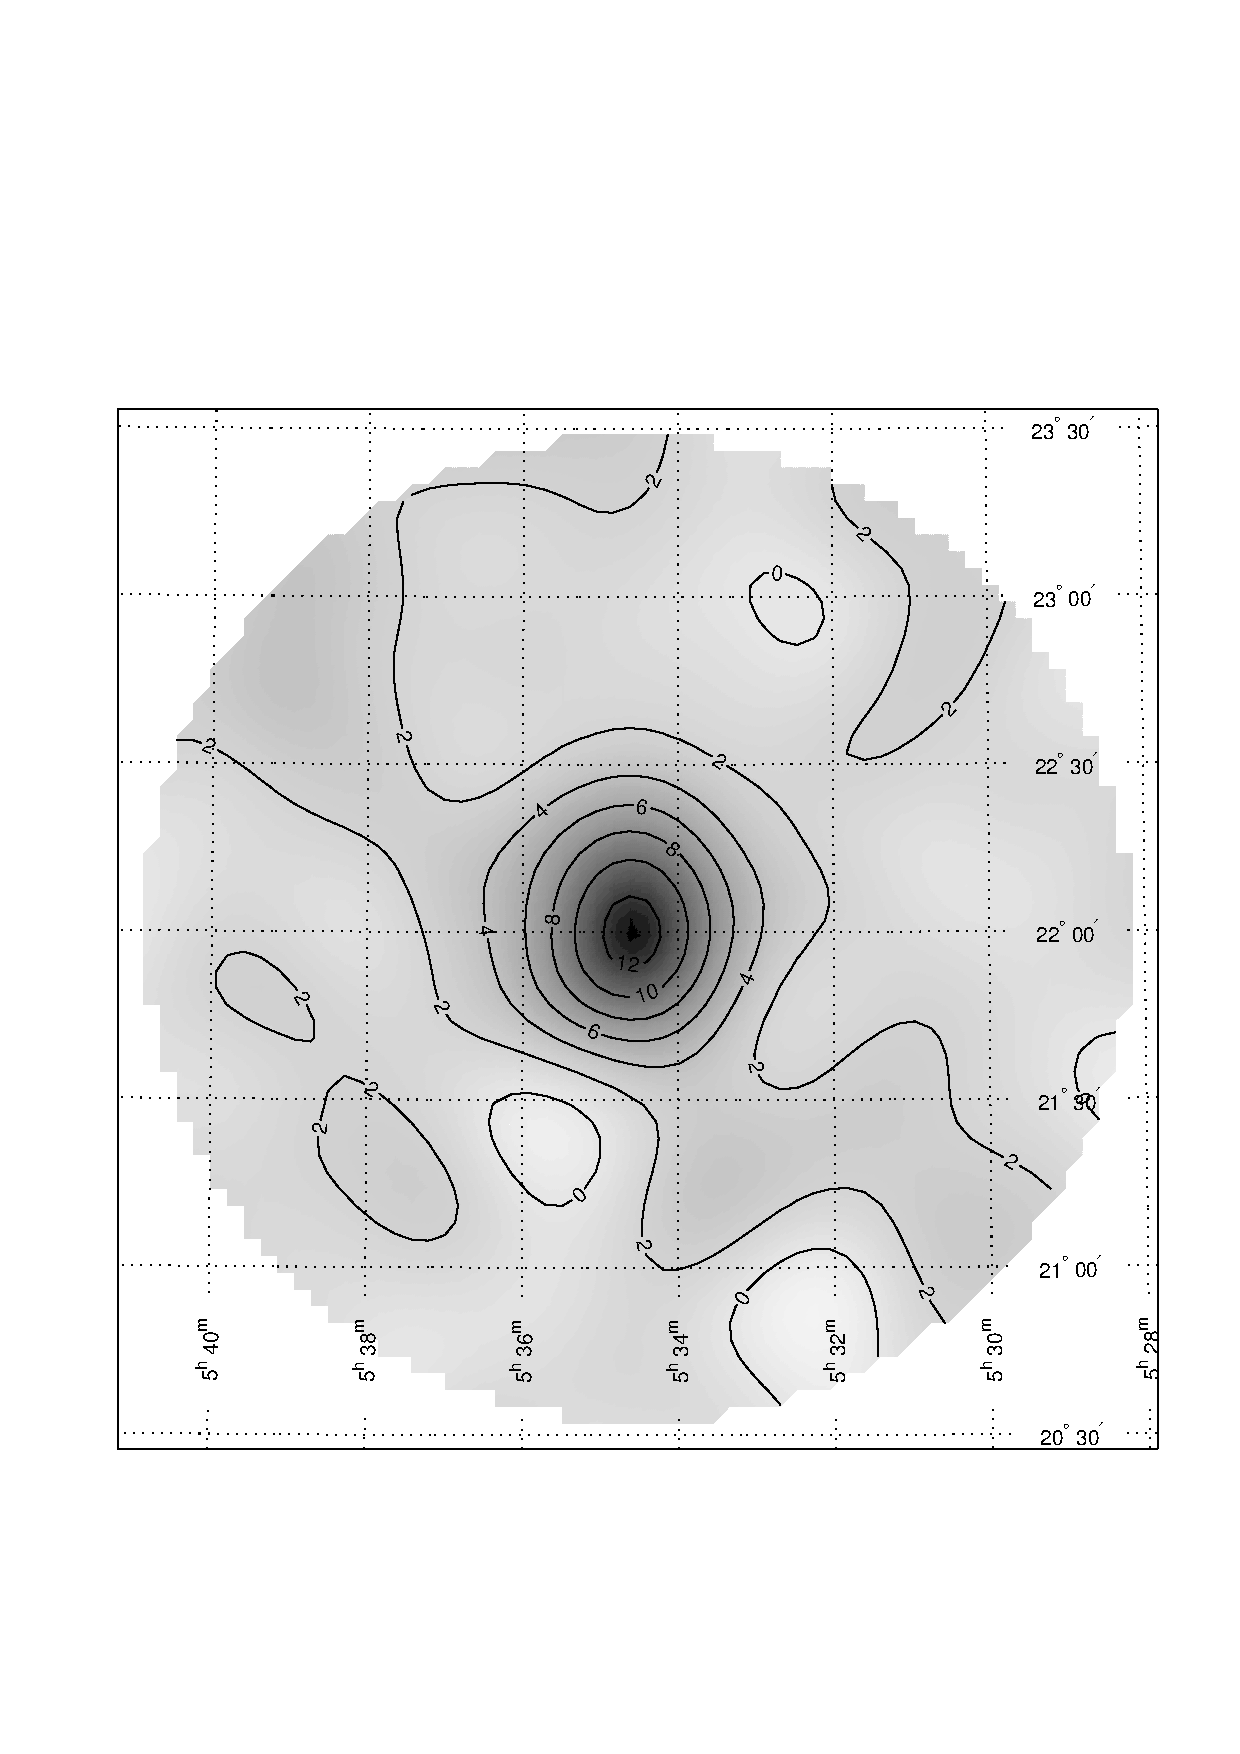
\includegraphics[draft=false]{plots/chap-analysis/crab_0_0_y0001_sig_bw.pdf}}%
\resizebox*{0.33\textwidth}{!}{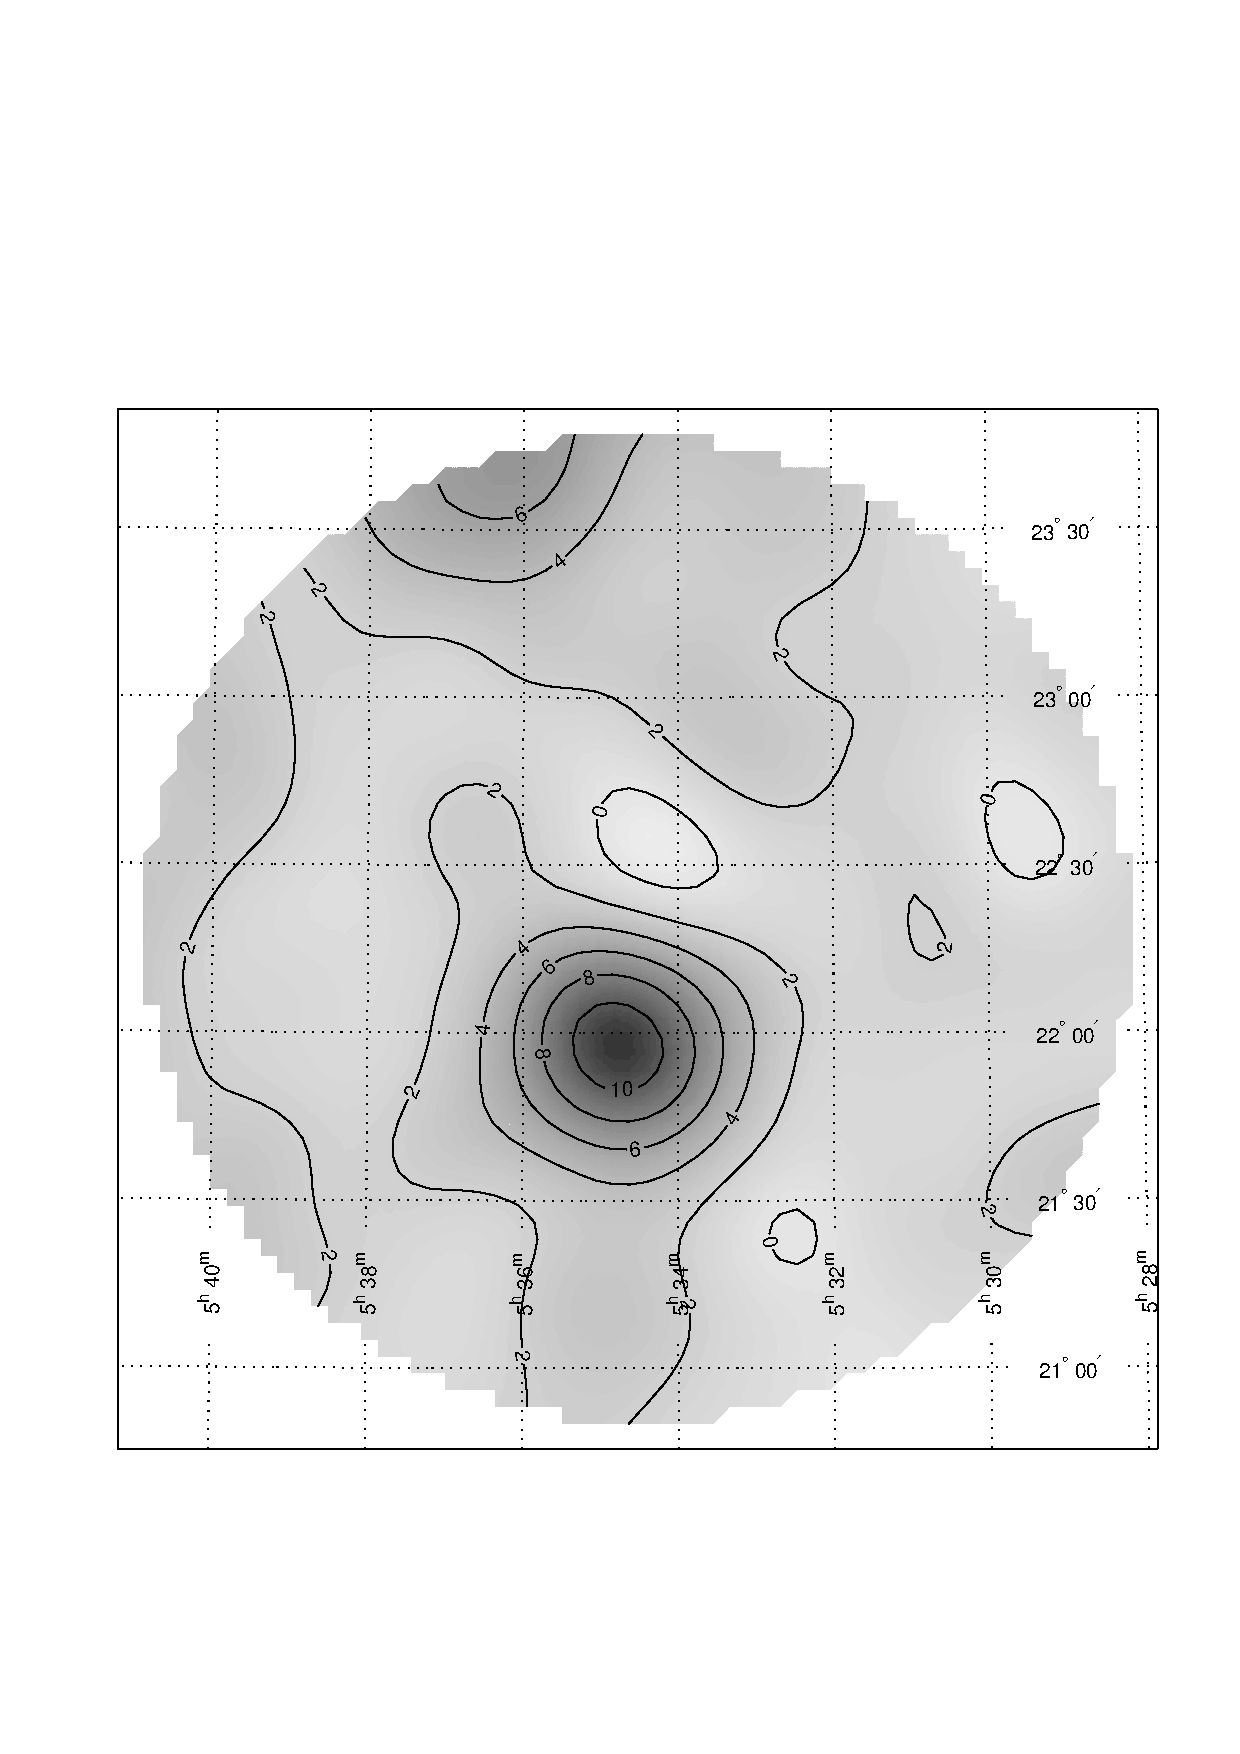
\includegraphics[draft=false]{plots/chap-analysis/crab_0_3_y0001_sig_bw.pdf}}%
\resizebox*{0.33\textwidth}{!}{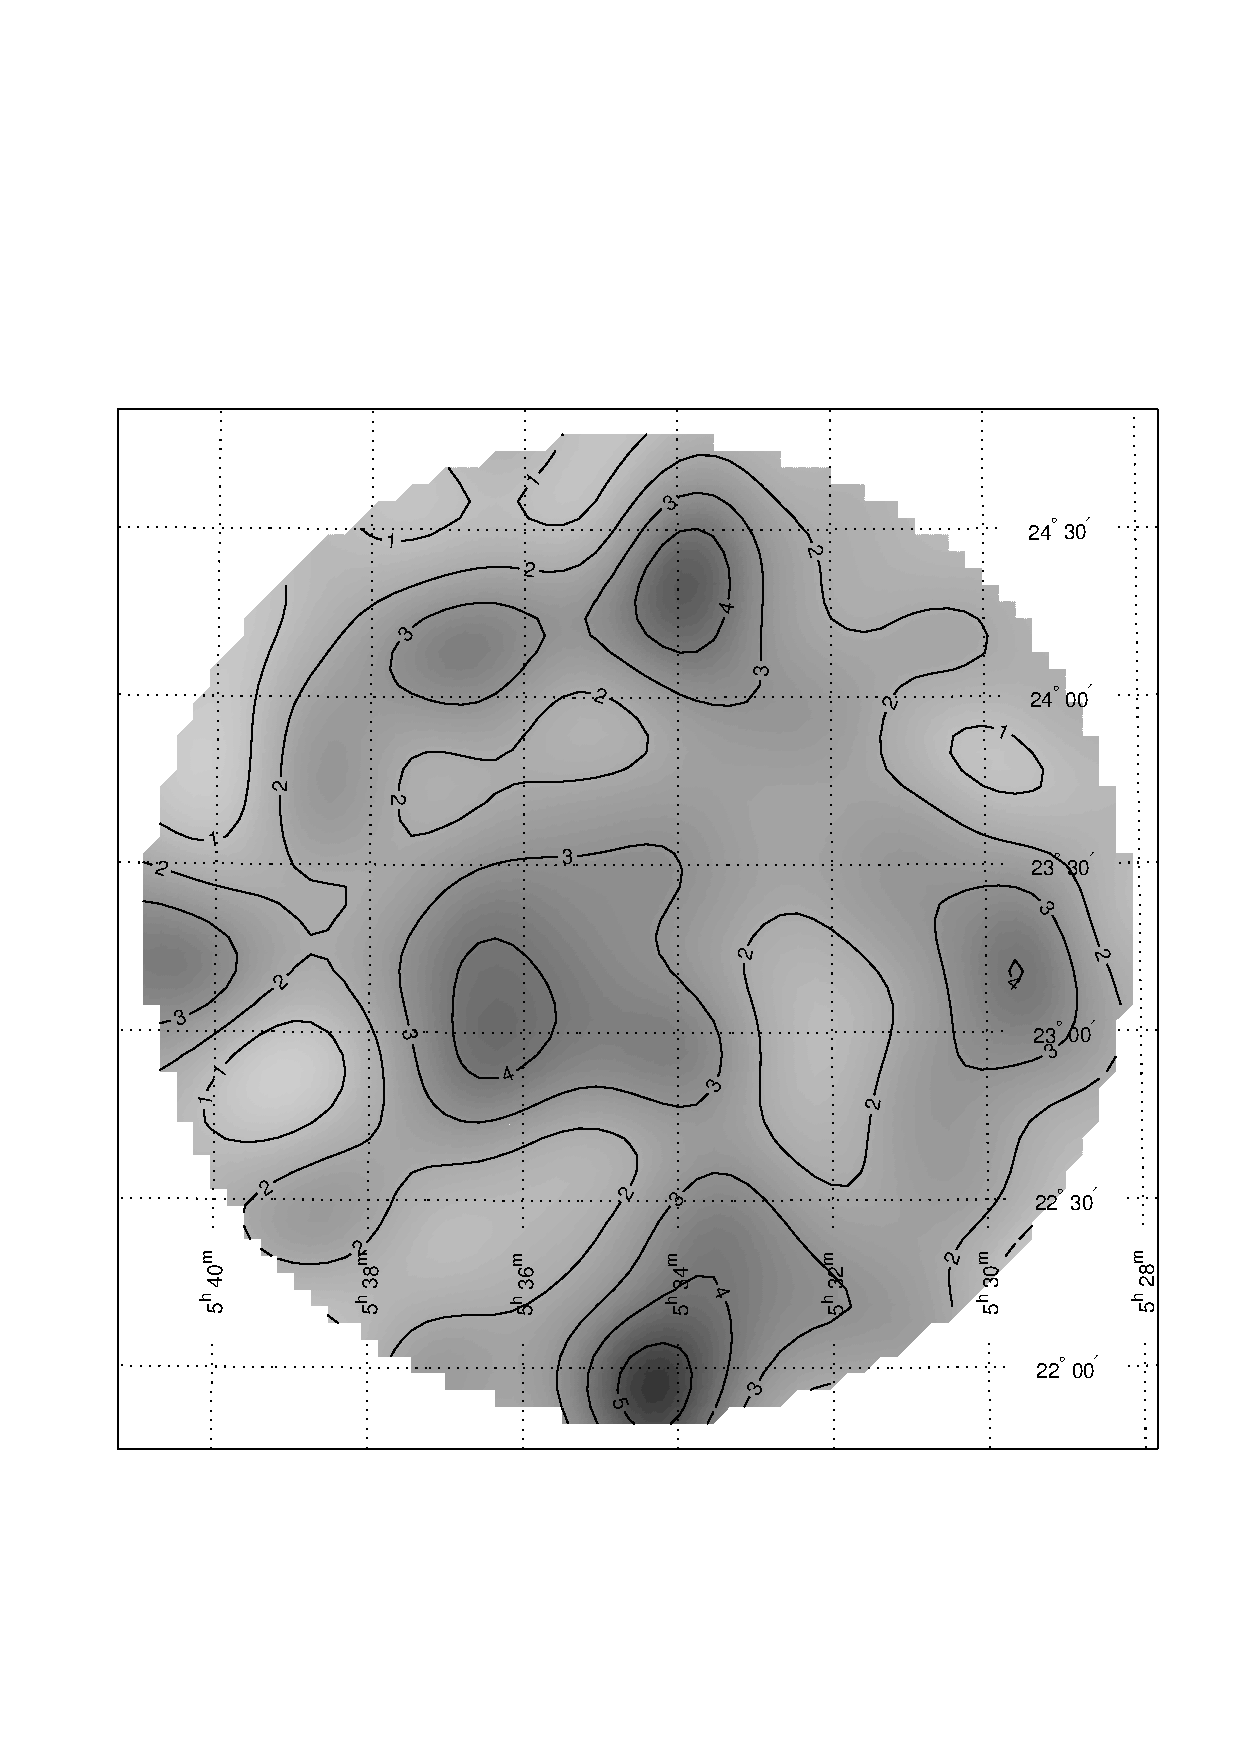
\includegraphics[draft=false]{plots/chap-analysis/crab_1_3_y0001_sig_bw.pdf}}}}
\caption{\label{FIG::ANALYSIS::2DSIGMA} Observations of the 
Crab Nebula, offset by varying amounts from the center of the field of 
view. The contours show detection significance. The observations at an 
offset of $1.3^\circ$ place the Crab outside of this.}
\end{figure}

Figure \ref{FIG::ANALYSIS::2DSIGMA} shows significance maps for the
Crab Nebula offset by three different amounts. In each of them the
Crab is clearly visible. At an offset of $0.3^\circ$ the \Gray
collection efficiency is $84$\% of what it is on axis.  At an offset
of $1.3^\circ$, with the source outside of the geometrical extent of
the camera, the efficiency is $30$\%. The significance map for this
data shows appreciable background contamination over the field due to
the simple reconstruction approach of assigning the arrival direction
of each photon to two points on the shower axis. More sophisticated
approaches can reduce such false sources
\citep{REF::LESSARD::2001APP}.

\begin{figure}[p]
\centerline{\resizebox*{\textwidth}{!}{\rotatebox{270}{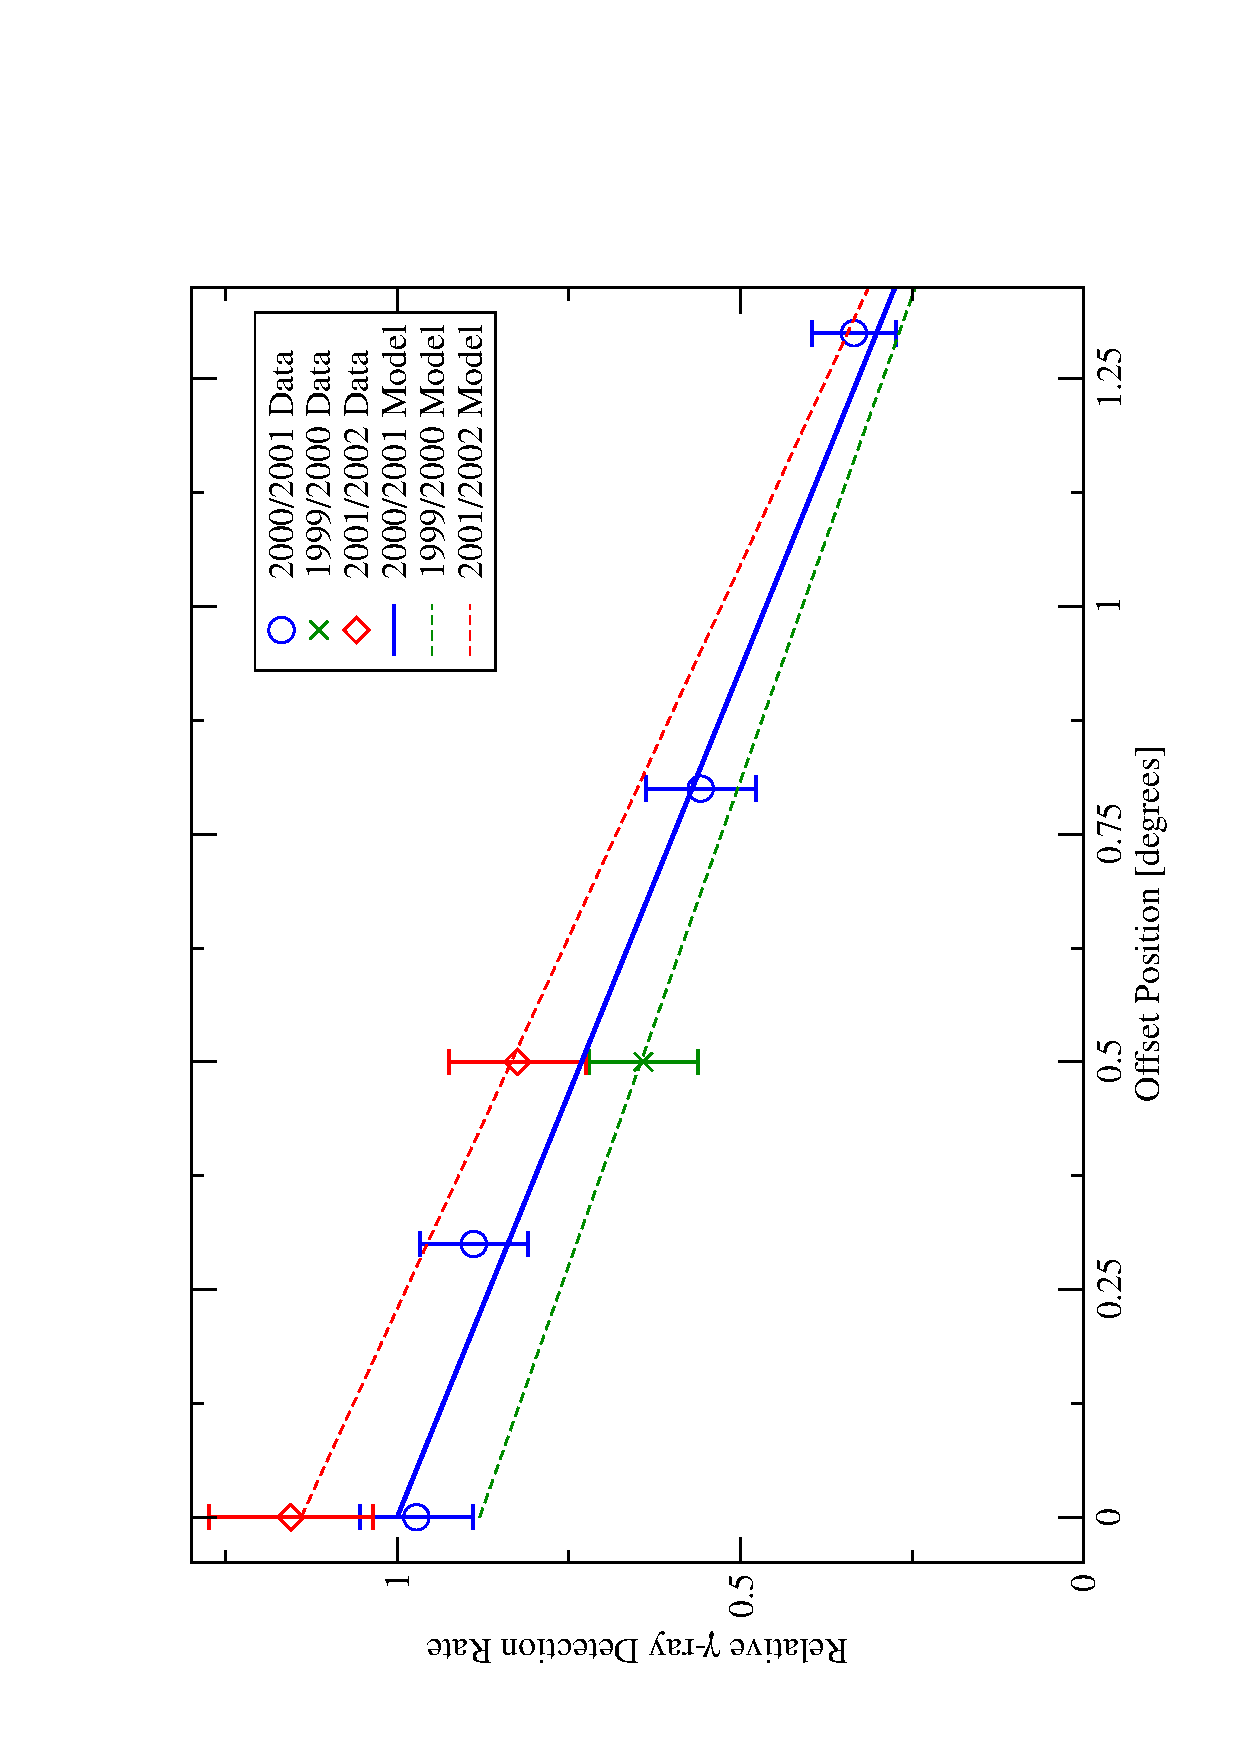
\includegraphics{plots/chap-analysis/rate_model.pdf}}}}
\caption{\label{FIG::ANALYSIS::2DRATE} Relative Crab detection rate as 
a function of source offset. The off-axis response can be fit by a 
straight line.}
\end{figure}

Figure \ref{FIG::ANALYSIS::2DRATE} shows the relative collecting
efficiency for offset sources. This curve is used to normalize
detected emission rates or upper limits to the Crab flux. 

\section{Significance of Observations}
\label{SEC::ANALYSIS::SIGNIFICANCE}

The calculated significance, $\sigma(\vec{r})$, described above,
corresponds to the confidence that the null hypothesis, i.e.\ that no
source is present at that point in the sky, is false. A large value of
significance can be thought of as giving a high confidence that a
source is present at the location. In the absence of any source,
$\sigma(\vec{r})$ should be distributed as Gaussian with unity width,
for any location in the field of view ($\vec{r}$) chosen a priori. To
ensure that the measurement of sigma is not biased, ``dark-field''
observations were analyzed. The analysis was applied to $240$
observations from 1999 to 2003 which were taken on regions of the sky
which are assumed to have no source present in them, i.e.\
observations on candidate point-source objects whose analysis did not
result in any significant excess. The significance of any excess (or
deficit) found in the center bin, $\sigma(\vec{0})$, of the sky map
from each of the observations is displayed in
figure~\ref{FIG::ANALYSIS::SIGMACENTER}.

\begin{figure}[p]
\centerline{\resizebox*{0.7\textwidth}{!}{\rotatebox{270}{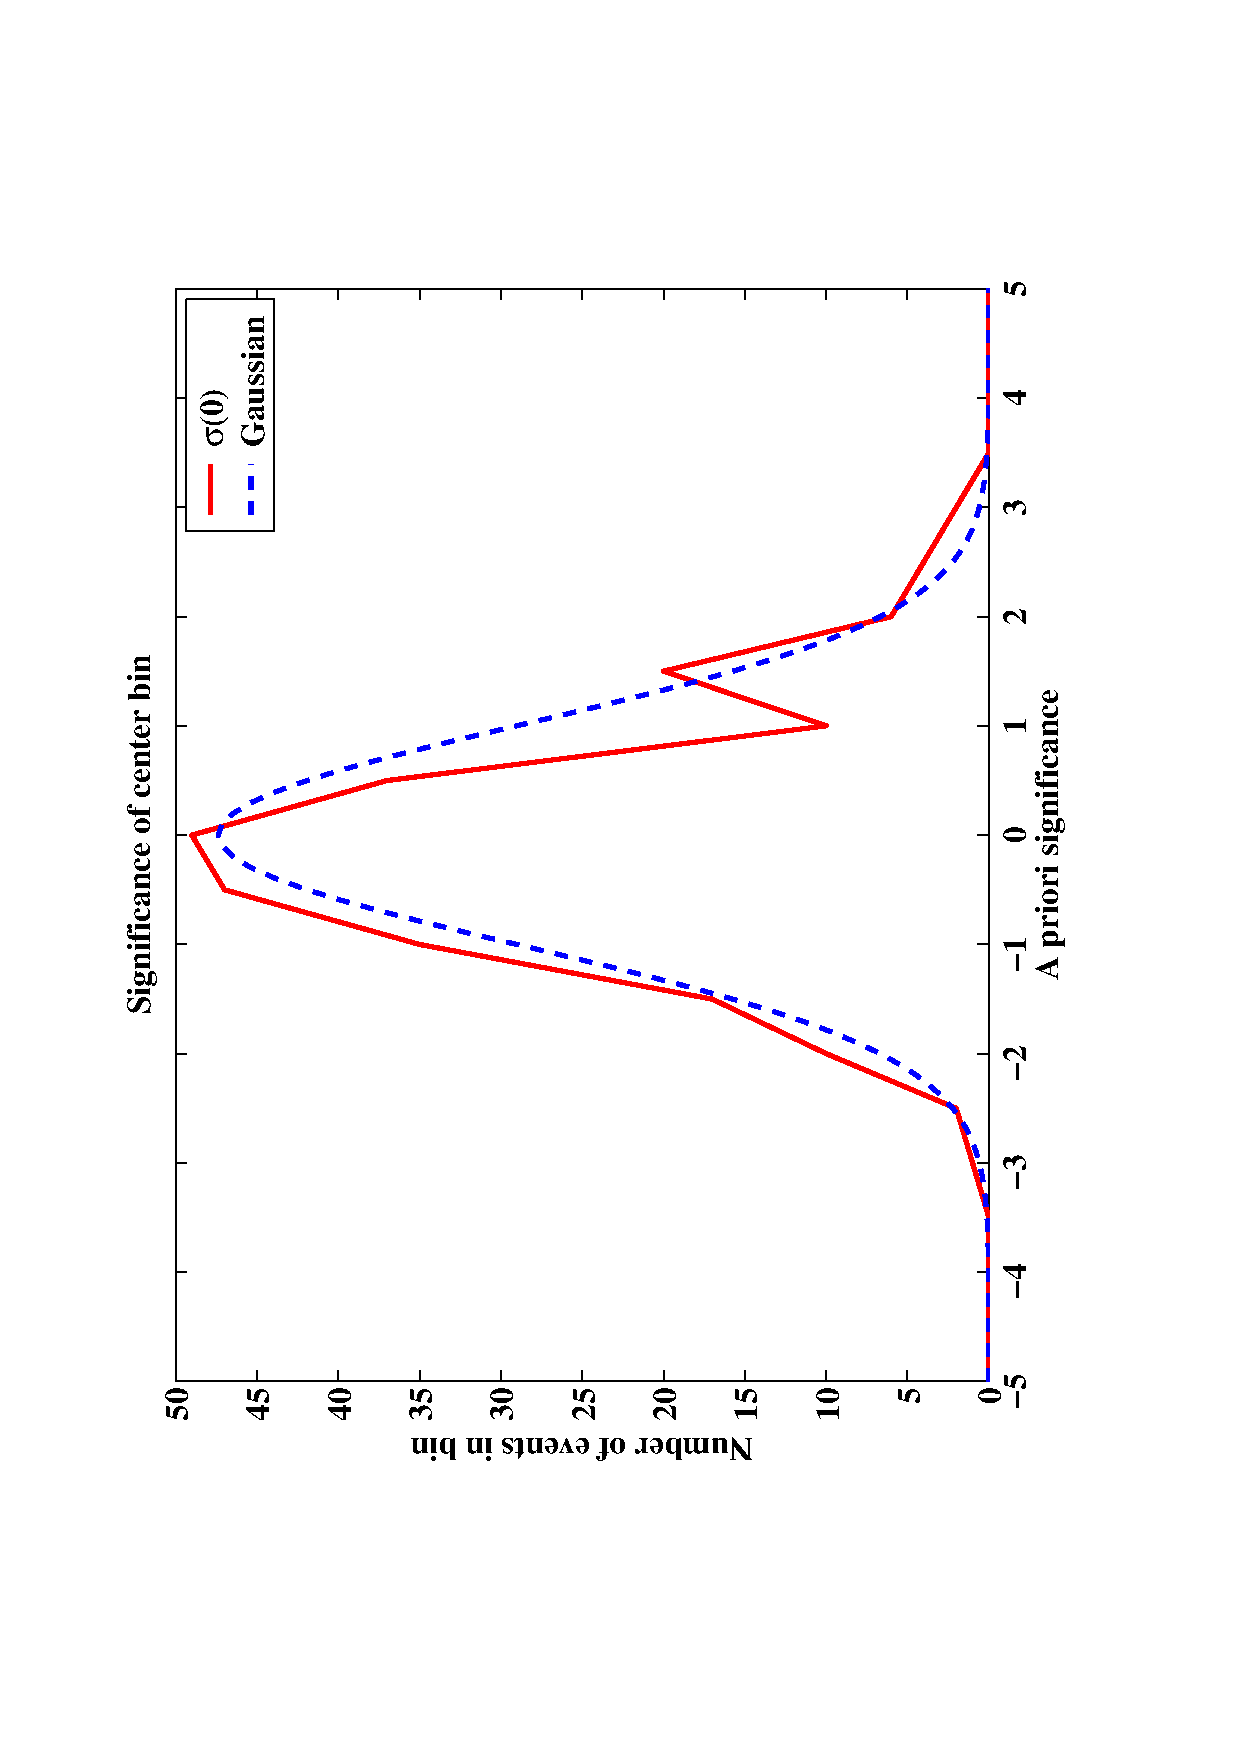
\includegraphics{plots/chap-analysis/sigma_center.pdf}}}}
\caption{\label{FIG::ANALYSIS::SIGMACENTER} Significance of 
excess (deficit) in counts in center bin of $240$ background observations. 
A Gaussian function of unity width, integrated over the binning size, 
is also shown.}
\end{figure}

\begin{figure}[p]
\centerline{\resizebox*{0.7\textwidth}{!}{\rotatebox{270}{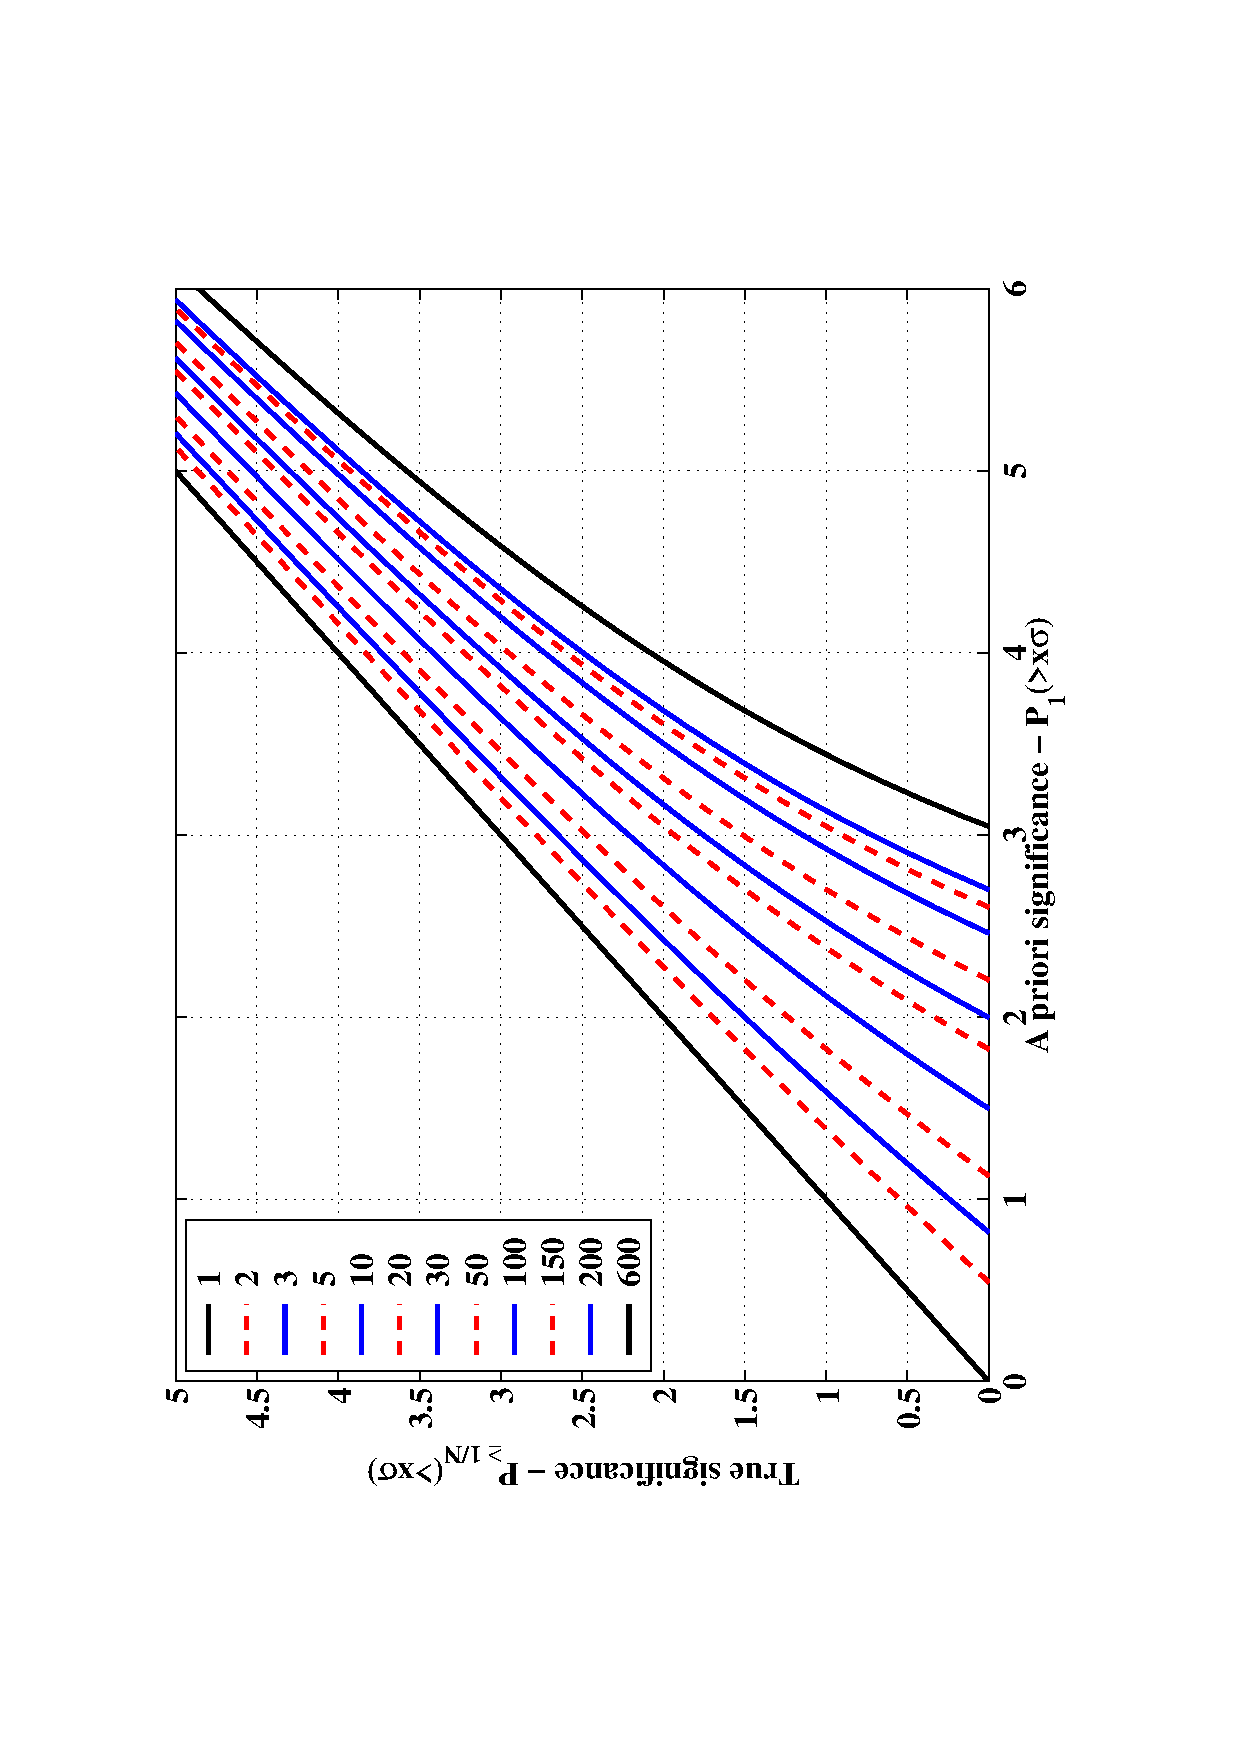
\includegraphics{plots/chap-analysis/sigma.pdf}}}}
\caption{\label{FIG::ANALYSIS::SIGMASIGMA} Probability of at 
least one from $N$ observations giving a result of $>x\sigma$ as 
compared with the probability of a single observation giving the same
result. Curves with increasing $N$, from 1 to 600, go from left to
right.}
\end{figure}

When the location of the source within the field of view is not known
in advance, the null hypothesis must be modified to require that no
source be present anywhere within the field of interest. To reject
this hypothesis a number of independent bins must be calculated and the
``true significance'' of the largest observed excess must be
determined. This ``true significance'' is different from the a priori
significance $\sigma(\vec{r})$ discussed up to this point. The
distribution of the function $\max{\sigma(\vec{r})}$ is not Gaussian
for maps which contain more than one independent bin. Since the term
``significance'' is usually associated with the Gaussian distribution
it is less confusing to refer instead to the probability that the null
hypothesis be true or false.

For a single observation, with Gaussian distribution, the probability
that a result of $>x\sigma$ will be observed, in the absence of a \Gray
source, is given by the error function,
\[P_1(>x\sigma) = \frac{1}{\sqrt{2\pi}}\int_{x}^{\infty}e^{-x'^2/2}\mathrm{d}x' = \{1-\mathrm{erf}(x/\sqrt{2})\}/2.\]
The probability of observing at least one result of $>x\sigma$ in $N$
independent observations, denoted $P_{\geq 1/N}(>x\sigma)$, is
calculated by noting that if such a result is not observed, it must be
the case that \textbf{all} $N$ observations have a result of
$\leq x\sigma$, which is simply the product of $N$ individual
probabilities $P_1(\leq x\sigma)$,
\[P_{\geq 1/N}(>x\sigma) = 1 - \{1-P_1(>x\sigma)\}^N.\]
It is conventional to claim the detection of a source when the null
hypothesis has been rejected at a $>4\sigma$ level
\citep{REF::WEEKES::1999SNOWBIRD}, assuming a Gaussian distribution.
Figure~\ref{FIG::ANALYSIS::SIGMASIGMA} shows how $P_{\geq
1/N}(>x\sigma)$ relates to $P_1(>x\sigma)$. It can be seen from the
figure that a $4\sigma$ Gaussian confidence level (on the y-axis)
corresponds to the probability of detecting at least one
$\sim4.6\sigma$ result with $N=10$ and increases to $\sim5.3\sigma$
for $N=600$.

To relate the curves in figure~\ref{FIG::ANALYSIS::SIGMASIGMA} to the
sky maps generated from real data, an equivalent number of independent
bins must be calculated. The individual bins in the 2-d histogram are
highly correlated, both through the smoothing applied to the image and
the inaccuracy in the reconstruction method. Since the reconstruction
method is difficult to characterize, as are the effects of the edge of
the camera, the number of independent bins in the image is difficult to
calculate. Two estimates can be made, the first by considering the
width of the smoothing and the size of the camera, the second by
fitting for $N$ in the distribution, $P_{\geq 1/N}(>x\sigma)$, of
maximum significances from the dark-field data described above.

For a 2-dimensional Gaussian smoothing function, $g(\vec{r};r_0)=
\exp(-r^2/2r_0^2)$, 50\% of the counts are contained in a region of
radius $r=0.206^\circ$ for $r_0=0.175^\circ$. An estimate of the number
of independent bins can be made for regions of the sky map of various
widths, given by $2R$, by taking the ratio of the area of the region
and the area under the Gaussian. To account for effects at the border
of the region of interest, a border of $0.206^\circ$ can be added, so
\[N \sim \frac{\pi\times(R+0.206^\circ)^2}{\pi\times(0.206^\circ)^2} =
\left(\frac{R}{0.206^\circ}+1\right)^2\]
The estimates for $N$ from this method, with and without the border
effect are shown in table~\ref{TABLE::ANALYSIS::NINDEPENDENT}.

To estimate the number of independent bins from the distribution of
the maximum significance in the dark field data,
\mbox{$\max(\sigma(\vec{r})\;;|\vec{r}|<R)$}, a maximum likelihood
approach is used. For any value of $R$, the size of the region of
interest, analysis of the $240$ dark fields result in a set of maximum
significances, $\{x^{(R)}_i\}=\{\,max(\sigma_i(\vec{r})\;;|\vec{r}|<R)\,\}$.
The likelihood that this set of observations are drawn from the 
probability distribution for $N$ independent Gaussian observations is
given by,
\[L(x^{(R)}_i\,|\,N) = \prod_{i=1}^{240}\left[\frac{\mathrm{d}P_{\geq
1/N}(>x\sigma)}{\mathrm{d}x}\right]_{x=x^{(R)}_i}\] Maximizing the log
likelihood, $\Lambda=\ln L$, gives the best estimate of the number of
independent bins for each region size, $N(R)$. 

Figure~\ref{FIG::ANALYSIS::2DSIGMADISTRIBUTIONS} shows the
experimental distributions for $R=0.38^\circ$, $R=0.55^\circ$ and
$R=1.10^\circ$. The theoretical distribution based on the most likely
value of $N(R)$ is also shown. It can be seen that in the
$R=1.1^\circ$ case, the fit is not particularly good, a result of the
broad tails on the experimental distribution. Also displayed on these
figures is the results of a simple Monte Carlo (MC) simulation of the
smoothing, as described in appendix~\ref{APP::SMOOTHING}. It can be
seen that the likelihood fit to the experimental results matches the
MC distributions well, with the MC distributions being slightly
wider. Figure~\ref{FIG::ANALYSIS::NINDEPENDENTLIKELIHOOD} shows the
function $N(R)$ plotted against the area of the region, $A\propto
R^2$. It can be seen that there is a roughly linear increase of $N$
with $A$, at least for
$R<0.9^\circ$. Table~\ref{TABLE::ANALYSIS::NINDEPENDENT} lists the
values of $N$ for the cases considered above.

\begin{figure}[p!]
%\begin{minipage}{0.33\textwidth}\centerline{$r<0.35^\circ$}\end{minipage}%
%\begin{minipage}{0.33\textwidth}\centerline{$r<0.55^\circ$}\end{minipage}%
%\begin{minipage}{0.33\textwidth}\centerline{$r<1.10^\circ$}\end{minipage}\\
\resizebox*{0.33\textwidth}{!}{\rotatebox{270}{\includegraphics[draft=false]{plots/chap-analysis/dof_exp_like_0_348.pdf}}}%
\resizebox*{0.33\textwidth}{!}{\rotatebox{270}{\includegraphics[draft=false]{plots/chap-analysis/dof_exp_like_0_550.pdf}}}%
\resizebox*{0.33\textwidth}{!}{\rotatebox{270}{\includegraphics[draft=false]{plots/chap-analysis/dof_exp_like_1_100.pdf}}}
\caption{\label{FIG::ANALYSIS::2DSIGMADISTRIBUTIONS} 
Experimental and best-fit distributions for 
$\max(\sigma(\vec{r})\;;|\vec{r}|<R)$, listed
for $R=0.38^\circ$, $R=0.55^\circ$ and $R=1.10^\circ$.}
\end{figure}

\begin{figure}[p!]
\centerline{\resizebox*{0.8\textwidth}{!}{\rotatebox{270}{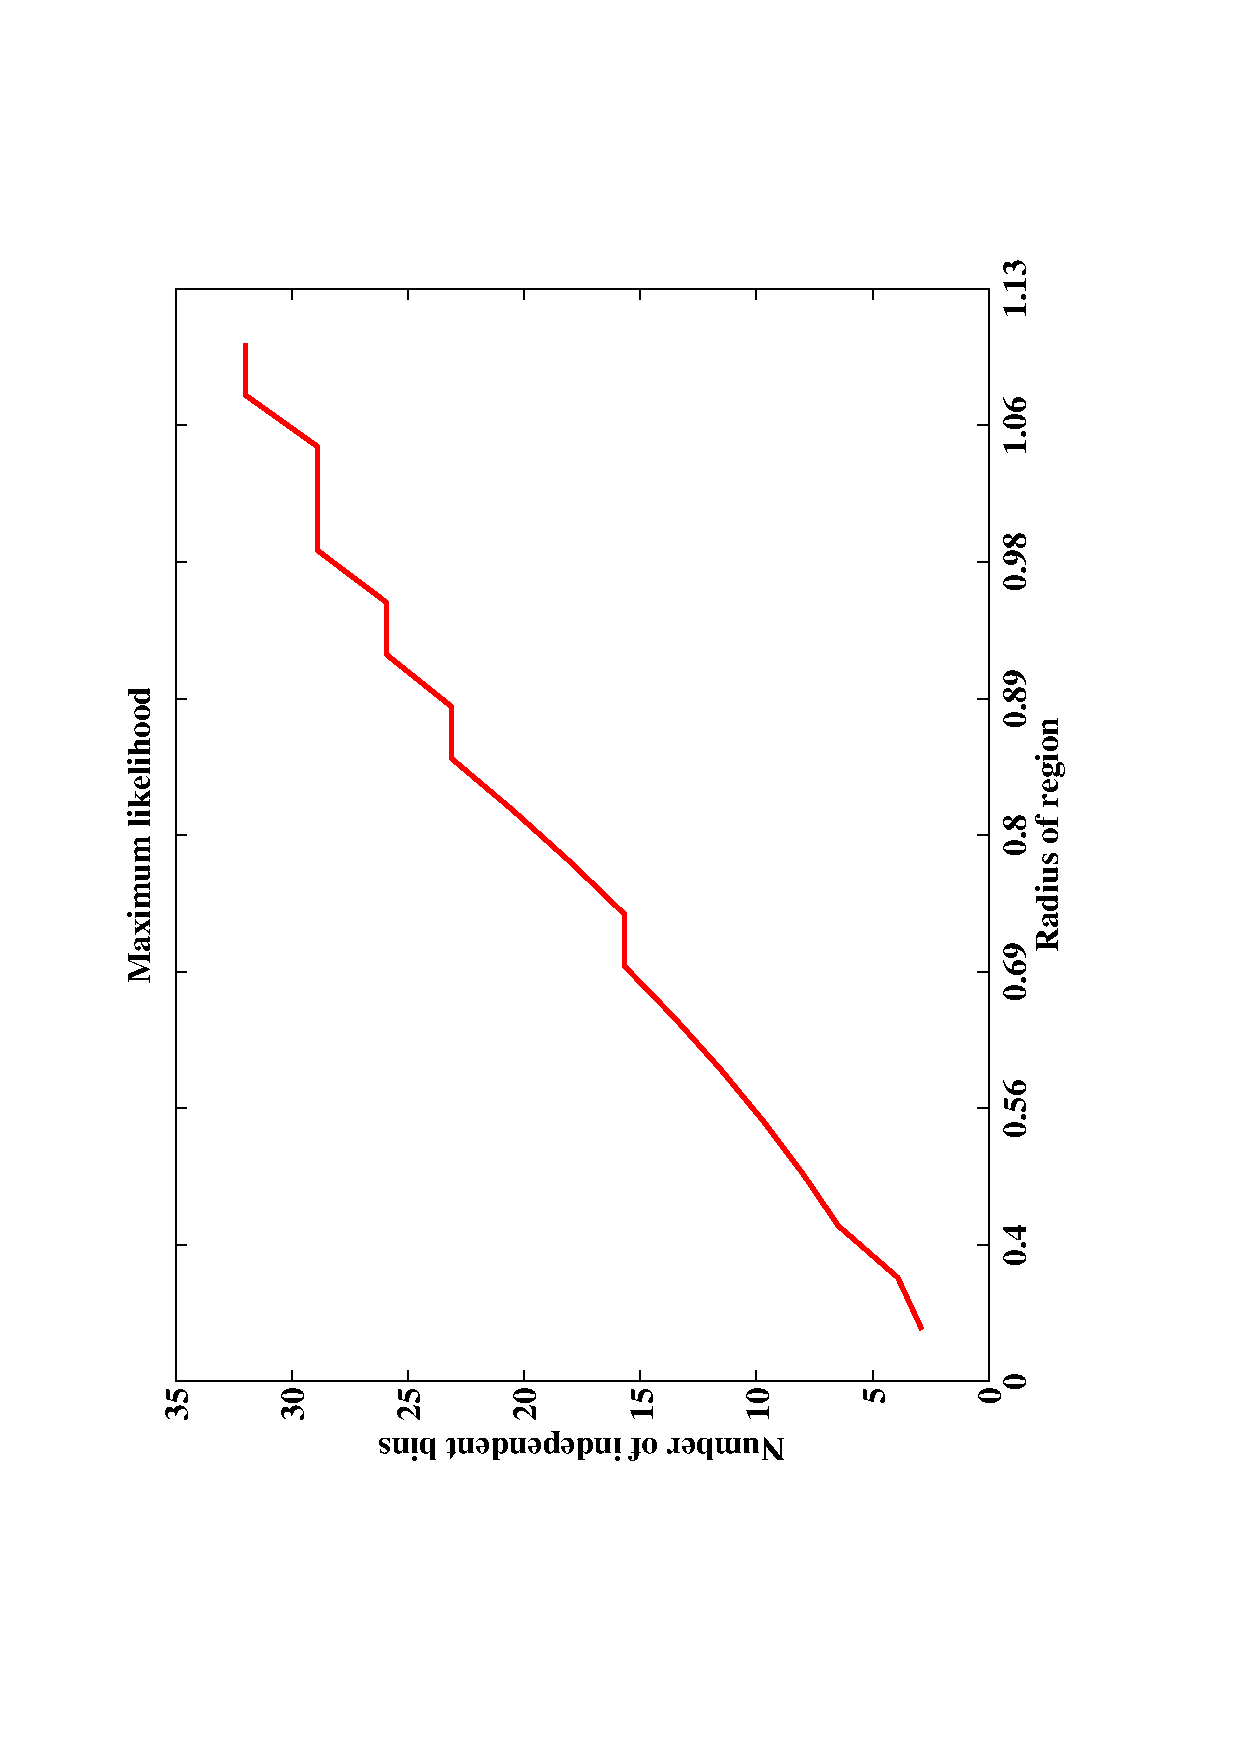
\includegraphics[draft=false]{plots/chap-analysis/dof_like.pdf}}}}
\caption{\label{FIG::ANALYSIS::NINDEPENDENTLIKELIHOOD} 
Maximum likelihood fit for $N(R)$ as a function of $A\propto R^2$.}
\end{figure}

\begin{table}[p]
\caption{\label{TABLE::ANALYSIS::NINDEPENDENT} Estimates 
for the number of independent bins, $N$, present in the region of 
a sky-map of area $\pi R^2$. Three estimates are given, the first 
two express the ratio of the areas of the region and the smoothing 
Gaussian. The final estimate is from a maximum likelihood fit to 
the distribution of maximum significance.}
\centerline{\begin{tabular}{llll}\hline
Method & $R=0.35^\circ$ & $R=0.55^\circ$ & $R=1.1^\circ$ \\\hline
Ratio of areas $(R/0.206)^2$    &  3 &  7 & 29 \\
Ratio of areas $(R/0.206+1)^2$  &  7 & 13 & 40 \\
Maximum likelihood fit          &  4 & 10 & 32 \\\hline
\end{tabular}}
\end{table}

When data from an unidentified EGRET source is analyzed, a map of (a
priori) significance is produced and the EGRET 95\% contour level
overlaid. The area of the region inside the contour can then be used
to calculate an equivalent number of independent bins, using
figure~\ref{FIG::ANALYSIS::NINDEPENDENTLIKELIHOOD}. This value can
then be used to calculate a significance level which is equivalent to
the accepted Gaussian $4\sigma$ confidence level. The map can then be
checked for emission from within the region of interest.

Additionally, the data can be tested to see whether they are
consistent with the null hypothesis that no emission is present in any
of the $18$ candidate fields considered in the survey. The value of
$N$ appropriate is $18\times N(1.1^\circ)\approx 600$, the number of
independent bins in the regions of the sky within $1.1^\circ$ of the
center (the region defined by the edge of the camera) of each $18$
field. A significance level, from
figure~\ref{FIG::ANALYSIS::SIGMASIGMA}, of $\sim5.3\sigma$ is required
to claim the null hypothesis is false with the required confidence.

\section{\Trk\ Analysis}
\label{SEC::ANALYSIS::TRACKING}

For objects whose location is well known, a simpler analysis technique
can be applied. The analysis can take advantage of the \Trk\ mode of
observation, giving twice the amount of on-source data over the \Pairs\
mode. As described above, the analysis takes advantage of the fact
that the candidate source is at the center of the field of view, which
allows events which are not consistent with having originated at the
center of the field of view to be eliminated. The selection is done on
the basis of the \textit{alpha} parameter; a cut of $\alpha<15^\circ$
was been found to be optimal. An estimate of the background is made
from the number of events which are not aligned with the center of the
field of view; those with $20^\circ<\alpha<65^\circ$ are
chosen. Assuming there are $N_{On}$ events with $\alpha<15^\circ$ and
$N_{Off}$ with $20^\circ<\alpha<65^\circ$, the excess counts is given
by,
\begin{equation}\label{EQN::ANALYSIS::TRKEXCESS}
\Delta N = N_\mathrm{On}-\rho\,N_\mathrm{Off}
\end{equation}
The constant $\rho$, termed the ``tracking ratio'', relates the number
of counts with $\alpha<15^\circ$ to the number with
$20^\circ<\alpha<65^\circ$ in the absence of a source. This constant
must be calculated independently with dark field observations. The
significance of the excess is given by propagation of errors,
\begin{equation}\label{EQN::ANALYSIS::TRKSIGMA}
\sigma = \frac{N_\mathrm{On}-\rho\,N_\mathrm{Off}}
{\sqrt{N_\mathrm{On}+\rho^2\,N_\mathrm{Off}}}
\end{equation}

This equation for significance is not completely correct for a number
of reasons. First, the value of $\rho$ calculated from dark field data
has an error associated with it, $\rho\pm\Delta\rho$. The calculation
of significance equation must account for this error, lowering the
significance somewhat. Additionally, as described in
\citet{REF::LIANDMA::1983APJ}, calculation of significance should be
based on a likelihood approach rather than the simple propagation of
errors above, which systematically underestimates the significance (in
the absence of $\Delta\rho$). The corrected equations for significance
are listed in appendix~\ref{APP::LIANDMA}. In practice, the
differences between the calculated values are small, and
equation~\ref{EQN::ANALYSIS::TRKSIGMA} can be employed.


%crab-9900-0.5  7.8  0.0269  0.0035  0.0351
%crab-0001-0.0  13.2  0.0417  0.0032  0.0491
%crab-0001-0.3  11.2  0.0371  0.0033  0.0448
%crab-0001-0.8  7.0  0.0234  0.0034  0.0312
%crab-0001-1.3  5.5  0.0131  0.0024  0.0188
%crab-0102-0.0  7.4  0.0278  0.0038  0.0366
%crab-0102-0.5  8.3  0.0345  0.0042  0.0443
%crab-0102-0.8  4.2  0.0195  0.0046  0.0302
%crab-0203-0.0  16.6  0.0311  0.0019  0.0355
%crab-0203-0.8  7.5  0.0241  0.0032  0.0316
%crab-0203-1.0  1.8  0.0056  0.0031  0.0130
%crab-0203-1.3  4.4  0.0129  0.0030  0.0199


%crab-9900-0.5  4.4  0.0047  0.0011  0.0072
%crab-0001-0.0  7.6  0.0059  0.0008  0.0077
%crab-0001-0.3  7.9  0.0060  0.0008  0.0078
%crab-0001-0.8  3.6  0.0033  0.0009  0.0054
%crab-0001-1.3  2.1  0.0017  0.0009  0.0037
%crab-0102-0.0  3.7  0.0045  0.0012  0.0074
%crab-0102-0.5  4.0  0.0054  0.0014  0.0086
%crab-0102-0.8  3.3  0.0060  0.0018  0.0102
%crab-0203-0.0  8.7  0.0056  0.0006  0.0071
%crab-0203-0.8  4.6  0.0051  0.0012  0.0078
%crab-0203-1.0  1.8  0.0020  0.0011  0.0047
%crab-0203-1.3  2.9  0.0030  0.0013  0.0062


\chapter{Observations}
\label{CHAP::OBSERVATIONS}

VHE observations of 19 unidentified EGRET sources are presented in this
chapter. The sources, listed in
table~\ref{TAB::OBSERVATIONS::CATALOGDATA}, and depicted in
figure~\ref{FIG::OBSERVATIONS::SOURCES}, are distributed across the
portion of the sky visible from southern Arizona, with seven at low
Galactic latitude ($b<5^\circ$), three at mid latitudes
($5^\circ<b<15^\circ$) and nine at high latitude. Eight have entries
in both the 3EG and GeV catalogs, two are listed only in the GeV
catalog, the remainder only in the 3EG catalog. The sample includes
3EG~J1835$+$5918 (\#14 in the table and figure), which has the hardest
spectrum among all unidentified 3EG sources (fifth hardest from all
3EG sources), a large 100\,MeV flux and a low variability
index. Included also is 3EG~J1337$+$5029 (\#12), which has the fourth
hardest spectrum from the unidentified sources. Five objects are
consistent with being in the Gould Belt, in particular \#4, \#5 and
\#6 lie approximately in the direction of the center of the Belt and
are each $>10^\circ$ from the Galactic plane.

\begin{figure}[h]
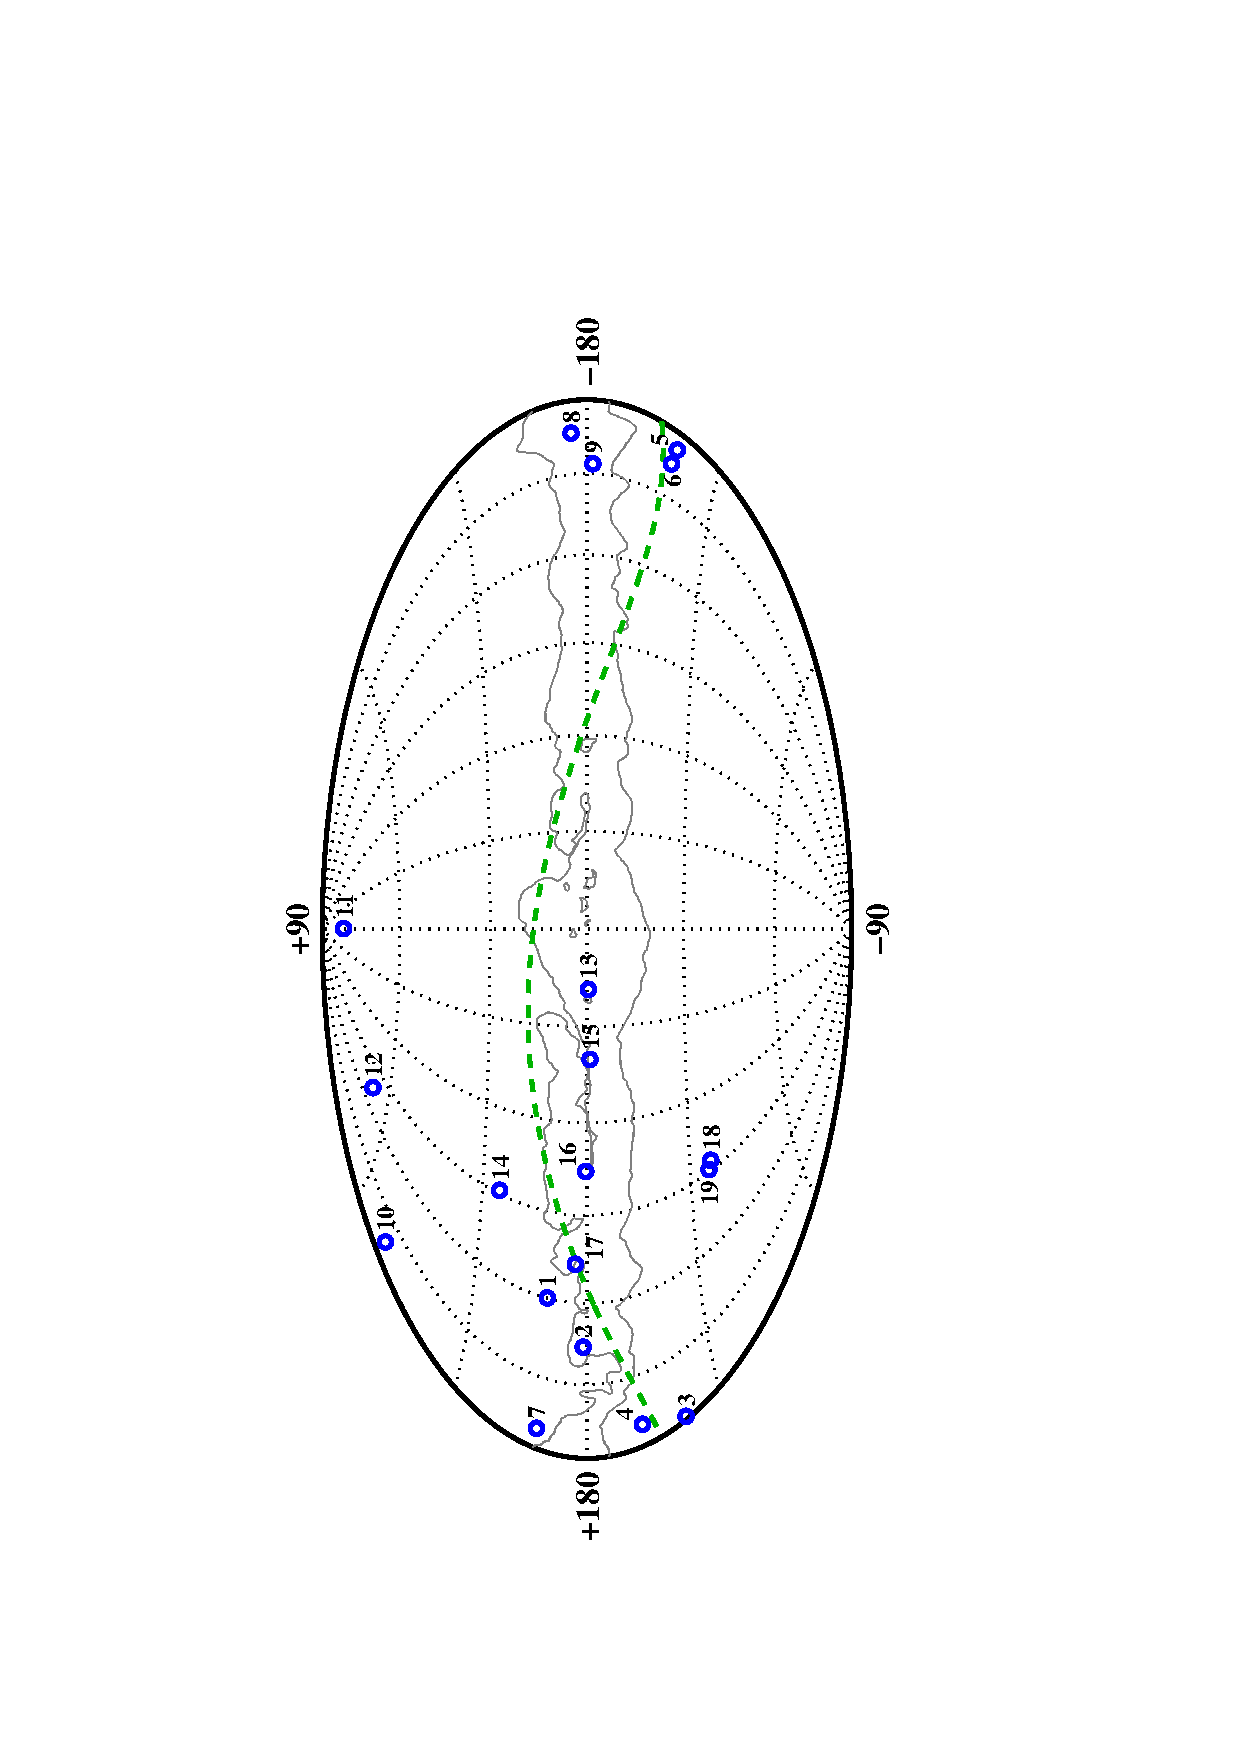
\includegraphics[angle=270,width=\textwidth]{plots/chap-observations/sources.pdf}
\caption{\label{FIG::OBSERVATIONS::SOURCES} The 19 unidentified EGRET
sources considered in this survey, plotted in Galactic coordinates. The
Milky Way and Gould Belt are also depicted, as described in 
chapter~\ref{CHAP::INTRODUCTION}. The candidate sources are labeled
by their positions in table~\ref{TAB::OBSERVATIONS::CATALOGDATA}.}
\end{figure}

\begin{table}[p]
\caption{\label{TAB::OBSERVATIONS::CATALOGDATA} Summary of the 3EG and 
GeV catalog entries for the 19 unidentified sources observed in the
survey.}
\centerline{\rotatebox{90}{\begin{minipage}{0.94\textheight}
\begin{tabular}{llllllllll}\hline
& Source Name & \multicolumn{2}{l}{Coordinates$^1$} &
\multicolumn{3}{l}{Third EGRET Catalog} &
\multicolumn{2}{l}{GeV Catalog} & Var. \\
& & & & Error$^2$ &
\multicolumn{2}{l}{Spectrum$^{3a}$} & Error & 
Flux$^{3b}$  & Indx.$^4$ \\
& & $b$ & $l$ & $\theta_{95}$ [$deg$] & $F\pm\Delta F$ & $\Gamma\pm\Delta\Gamma$ & 
$\theta_{95}$ [$deg$] & $F\pm\Delta F$ & $\delta$ \\\hline
1  & 3EG~J0010$+$7309 &  $10.56$ & $119.87$ & 0.25$\times$0.22 &  42.3$\pm$5.5 & 1.85$\pm$0.10 & 0.43             &  5.8$\pm$1.2 & 0.26 \\
2  & 3EG~J0241$+$6103 &   $0.99$ & $135.85$ & 0.21$\times$0.15 &  69.3$\pm$6.1 & 2.21$\pm$0.07 & 0.31             &  6.9$\pm$1.3 & 0.38 \\
3  & 3EG~J0423$+$1707 & $-22.21$ & $178.68$ & 0.88$\times$0.65 &  15.8$\pm$2.7 & 2.43$\pm$0.21 & -                &  -           & 0.42 \\
4  & GeV~J0433$+$2907 & $-12.58$ & $170.50$ & 0.19$\times$0.16 &  22.0$\pm$2.8 & 1.90$\pm$0.10 & 0.35             &  3.3$\pm$0.7 & 0.40 \\
5  & 3EG~J0450$+$1105 & $-20.55$ & $187.89$ & 0.65$\times$0.61 &  14.9$\pm$2.5 & 2.27$\pm$0.16 & -                &  -$^5$       & 1.13 \\
6  & GeV~J0508$+$0540 & $-19.81$ & $195.32$ & -                &  -            & -             & 0.62             &  1.4$\pm$0.4$^6$ & -$^7$\\
7  & 3EG~J0613$+$4201 &  $11.45$ & $171.38$ & 0.66$\times$0.46 &   9.0$\pm$2.3 & 1.92$\pm$0.26 & 0.65             &  1.8$\pm$0.6$^6$ & 0.72 \\
8  & 3EG~J0628$+$1847 &   $3.64$ & $193.60$ & 0.66$\times$0.49 &  23.9$\pm$4.0 & 2.30$\pm$0.10 & -                &  -           & -$^8$ \\
9  & 3EG~J0634$+$0521 &  $-1.22$ & $206.15$ & 0.85$\times$0.50 &  15.0$\pm$3.5 & 2.03$\pm$0.26 & -                &  -$^5$       & $<$0.88 \\
10 & 3EG~J1009$+$4855 &  $52.15$ & $166.93$ & 1.12$\times$0.80 &   4.8$\pm$1.4 & 1.90$\pm$0.37 & -                &  -           & $<$0.94 \\
11 & 3EG~J1323$+$2200 &  $81.15$ & $359.63$ & 0.52$\times$0.43 &   5.2$\pm$1.6 & 1.86$\pm$0.35 & -                &  -$^5$       & 1.09 \\
12 & 3EG~J1337$+$5029 &  $65.06$ & $105.18$ & 0.77$\times$0.66 &   9.2$\pm$2.6 & 1.83$\pm$0.29 & -                &  -           & 0.53 \\
13 & 3EG~J1826$-$1302 &  $-0.42$ &  $18.41$ & 0.55$\times$0.39 &  46.3$\pm$7.3 & 2.00$\pm$0.11 & 0.32             &  9.9$\pm$1.7 & 0.88 \\
14 & 3EG~J1835$+$5918 &  $25.08$ &  $88.74$ & 0.16$\times$0.13 &  60.6$\pm$4.4 & 1.69$\pm$0.07 & 0.27             & 10.2$\pm$1.4 & 0.15 \\
15 & GeV~J1907$+$0557 &  $-0.88$ &  $40.08$ & -                &  -            & -             & 0.38$\times$0.28 &  9.2$\pm$1.9 & -$^7$ \\
16 & GeV~J2020$+$3658 &   $0.24$ &  $75.29$ & 0.35$\times$0.26 &  59.1$\pm$6.2 & 1.86$\pm$0.10 & 0.28$\times$0.21 & 11.2$\pm$1.5 & 0.36 \\
17 & 3EG~J2227$+$6122 &   $3.19$ & $106.55$ & 0.50$\times$0.41 &  41.3$\pm$6.1 & 2.24$\pm$0.14 & 0.54             &  3.9$\pm$1.2$^6$ & 0.20 \\
18 & 3EG~J2248$+$1745 & $-36.15$ &  $86.00$ & 1.14$\times$0.78 &  12.9$\pm$3.5 & 2.11$\pm$0.39 & -                &  -           & 0.65 \\
19 & 3EG~J2255$+$1943 & $-34.35$ &  $89.85$ & 2.67$\times$2.33 &   5.8$\pm$2.8 & 2.36$\pm$0.61 & -                &  -           & 1.18 \\\hline
\end{tabular}\\[1.2ex]
\centerline{\footnotesize{\begin{tabular}{rp{0.9\textwidth}}
$^1$ & Galactic coordinates from the 3EG or GeV catalog as 
appropriate.\\
$^2$ & Elliptical fits to 95\% error contours for 3EG sources 
from \citet{REF::MATTOX::APJS2001}.\\
$^3$ & Flux at energies greater than (a) 100\,MeV and (b) 
1\,GeV in units of $10^{-8}$\,cm$^{-2}$s$^{-1}$.\\
$^4$ & Variability index from \citet{REF::NOLAN::APJ2003}, higher
values indicate more source variability.\\
$^5$ & Listed as source of repeating weak outbursts of GeV \Grays
\citep[Table~2 of][]{REF::MACOMB::ICRC1999}.\\
$^6$ & Listed as a low-significance source of GeV \Grays in 
table~2 or 3 of \citet{REF::LAMB::APJ1997}.\\
$^7$ & \citet{REF::NOLAN::APJ2003} present variability indices 
for 3EG sources only.\\
$^8$ & As noted in \citet{REF::NOLAN::APJ2003}, 3EG~J0628$+$1847 
failed a consistency check during the analysis. 
\end{tabular}}}
\end{minipage}}}
\end{table}

\section{Individual observations}

Details and results of the observations are presented below, with a
discussion of each candidate source and possible counterparts in the
fields of view. For each object, with the exception of GeV~J0508$+$0540,
a two dimensional analysis has been performed and a map of the excess
(or deficit) of {\Grayc}-like events produced. For objects where a
significant excess of events is detected, a map of the significance of
the emission is presented. For those without a significant excess,
i.e.\ those which do not have an excess at a $3\sigma$ level or
higher, a map of the upper limit of VHE \Gray emission is presented,
at a 99\% confidence level. The maps are overlayed with the 3EG error
contours\footnote{The contours were extracted from the on-line version
of the catalog which contains maps of the $(TS)^{1/2}$ likelihood
statistic} at the 50\%, 69\%, 95\% and 99\% confidence level, as
described by \citet{REF::MATTOX::APJ1996}. For GeV sources, the 95\%
error ellipse is shown, based on the parameters in the catalog.  From
each of these maps, the maximum upper limit within the 3EG (or GeV)
error-box is presented, corresponding to a conservative VHE upper
limit for the HE \Gray source. For each object that has potentially
interesting counterparts at other wavelengths, such as radio and x-ray
counterparts suggested in the literature, upper limits are also
presented for emission from the location of the possible counterparts;
these limits are generally lower than the limit on emission from the
entire error-box. Finally, for the sources with an entry in the 3EG
catalog, the \Gray spectrum is shown, extrapolated to 1\,TeV, with the
VHE upper limit for the error-box overlaid.

\subsection{3EG~J0010$+$7309}

The 3EG source J0010$+$7309 has long been suggested as possibly
associated with the supernova CTA~1, G119.5$+$10.2 in
\citet{REF::GREEN::WEB2001}, on the basis of its position. The
first images of CTA~1 at x-ray energies were recorded with the ROSAT
instrument; the source has been well studied with later x-ray
instruments, such as ASCA and XMM-Newton
\citep{REF::SEWARD::APJ1995, REF::SLANE::APJ1997, REF::SLANE::APJ2004}.
The observations indicate that the x-ray emission from CTA~1 must be
described by three components; the first is a thermal, shell-type,
component associated with the Sedov expansion of the remnant into the
inter-stellar medium (ISM), which appears to be occurring in a region
of low density. The shell-type nebula is large,
$\sim107$\,arcmin in diameter, and $1.4\pm0.3$\,kpc.\ in
distance. There is a ``blow-out'' region in the north of the nebula
where the nebula has evidently expanded quickly into a region of
particularly low density. The second x-ray component is evident as
a region of bright, non-thermal emission at the center of the
nebula. This emission is consistent with synchrotron emission from a
central PWN, with a power-law spectral index of 2.3 and total x-ray
luminosity of $L_\mathrm{X}=5.6\times10^{33}$\,erg\,s$^{-1}$. Finally,
ROSAT detected a non-thermal compact point source, RX~J0007.0$+$7302,
which may be associated with a pulsar at the center of the
nebula, although no pulsations have been detected in radio or
x-rays. \citet{REF::SLANE::APJ2004} report on
XMM observations of the compact source; its spectrum is
best fit by a power-law with index of 1.5 and total luminosity of
$L_\mathrm{X}=4.7\times10^{31}$\,erg\,s$^{-1}$.

The \Gray source has a large, steady $>$100\,MeV flux, a hard spectrum
of $\Gamma=1.85$, with possible evidence of softening above 2\,GeV and
a low variability index of
$\delta=0.26$. \citet{REF::BRAZIER::MNRAS1998} suggest that the \Grays
are most likely associated with the compact source which lies within
the 95\% confidence contour of the EGRET observations.  As noted by
\citet{REF::SLANE::APJ2004}, the power-law x-ray spectrum of the
compact source can be extrapolated to \Gray energies without a
spectral break. Other compact x-ray sources in the region are
suggested as possible counterparts by
\citet{REF::SEWARD::APJ1995}; \citet{REF::BRAZIER::MNRAS1998} dismiss
all but RX~J0010$+$7309.

\begin{figure}[t]
\resizebox*{\textwidth}{!}{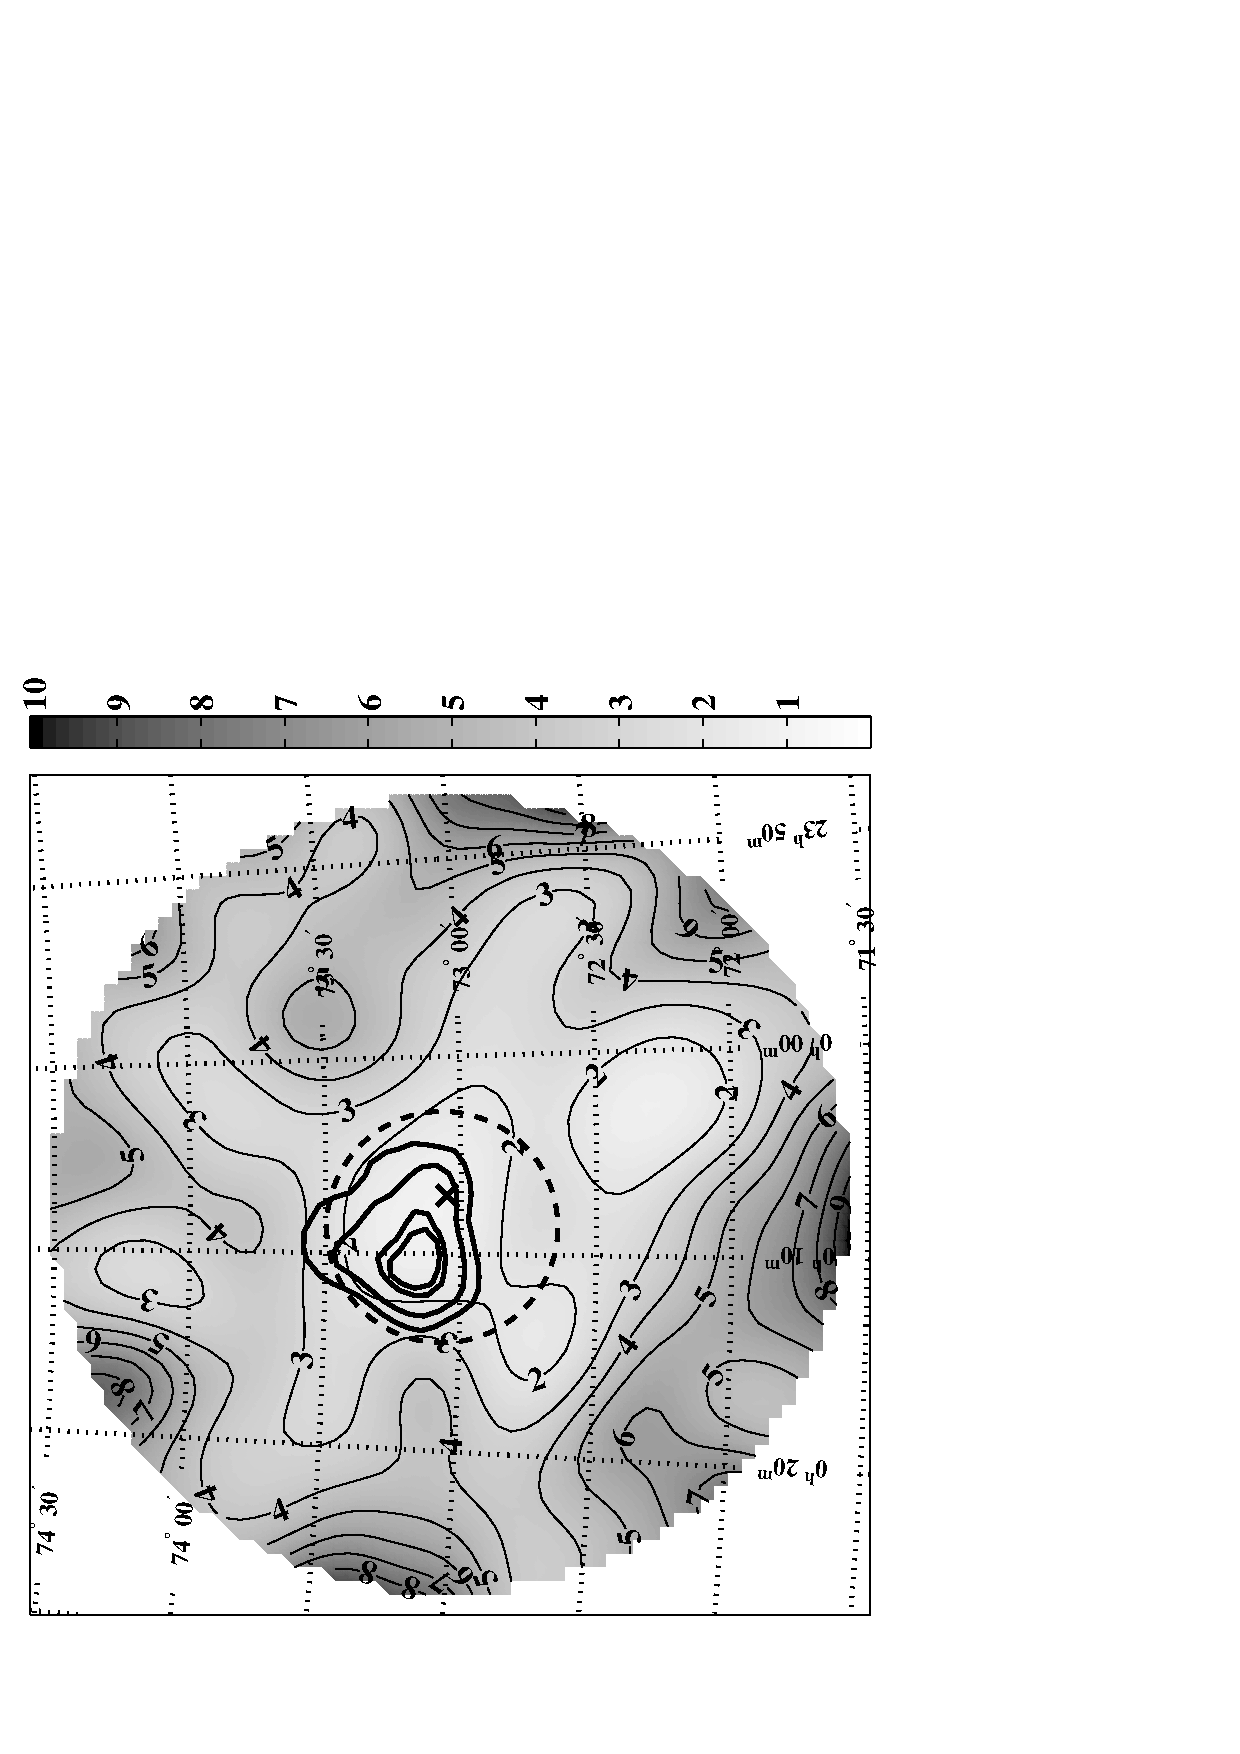
\includegraphics[draft=false,width=\textwidth,angle=270]{plots/chap-observations/loenergy/J0010+7309_sul_conv_bw.pdf}\includegraphics[width=\textwidth,angle=270]{plots/chap-observations/spectra/3EG_J0010+7309.pdf}}
\caption{\label{FIG::OBSERVATIONS::J0010} (Left) Limits on emission from 
3EG J0010$+$7309 in units of $10^{-11}$\,cm$^{-2}$\,s$^{-1}$. The 3EG
error contours are overlaid as heavy lines, the GeV catalog contour is
shown as a broken circle. (right) Spectrum from the on-line version of
the 3EG catalog with the limit at 350\,GeV.}
\end{figure}

The VHE observations reported here consist of a combined 195\,min.\
exposure on the source, pointed at the center of the nebula, offset by
0.27 degrees from the center of the 3EG source. The data were taken
during late 1999. No emission is detected at a significant level, an
upper limit on emission from anywhere within the 95\% error circle of
$F_{(>350\,\mathrm{GeV})}<2.2\times10^{-11}$\,cm$^{-2}$\,s$^{-1}$ is
calculated. Figure~\ref{FIG::OBSERVATIONS::J0010} shows the map of the
upper limit of point source emission from the region and the 3EG
power-law spectrum extrapolated to 350\,GeV, with the upper limit
superimposed. It is clear from the diagram that extrapolating the
EGRET power-law to the VHE regime is in conflict with these
observations by an order of magnitude. A cut-off in the spectrum is
required to reconcile the observations. Some evidence for this cut-off
is also visible in the highest energy bins of the EGRET spectrum. The
cut-off supports the supposition that the \Grays originate from a
pulsar. The upper limit from RX~J0007.0$+$7302, whose location is
marked with an ``X'' in figure~\ref{FIG::OBSERVATIONS::J0010}, is
$F_{(>350\,\mathrm{GeV})}<1.1\times10^{-11}$\,cm$^{-2}$\,s$^{-1}$.

\begin{table}[t]
\caption{\label{TAB::OBSERVATIONS::J0010} Upper limits for candidates
in 3EG~J0010$+$7309 field.}
\centerline{\begin{tabular}{lllll}\hline
Source Name & \multicolumn{2}{l}{Coordinates} & Extent & Upper Limit \\
& $\alpha_{2000}$ & $\delta_{2000}$ & deg & $\times10^{-11}$\,cm$^{-2}$\,s$^{-1}$\\\hline
3EG~J0010$+$7309     & $00^h09^m36.6^s$ & $+73^\circ10^{\prime}57.4^{\prime\prime}$ & 0.25$\times$0.22 & 2.2 \\
RX~J0007.0$+$7302    & $00^h07^m02.2^s$ & $+73^\circ03^{\prime}07.1^{\prime\prime}$ & -                & 1.1 \\\hline
\end{tabular}}
\end{table}

\subsection{3EG~J0241$+$6103}

First detected by the COS-B instrument, and designated as 2CG~135$+$01,
the \Gray source 3EG~J0241$+$6103 has been the subject of much study
over the past 25 years. On the basis of the COS-B position, the source
was been associated with the quasar QSO~4U0241$+$61, at redshift
$z=0.0438$, \citep{REF::MARASCHI::NATURE1978,
REF::APPARAO::NATURE1978} and with the non thermal radio source
GT~0236$+$610 \citep{REF::GREGORY_TAYLOR::NATURE1978,
REF::HERMSEN::NATURE1977}. Observations with EGRET refined the
position estimate, and eliminated the possible association with the
quasar \citep{REF::KNIFFEN::APJ1997}, which lies over a degree away.
The non-thermal radio source quickly came to be associated with the
binary system LSI~$+$61$^\circ$303 \citep{REF::GREGORY::AJ1979}, an
unusual object which has been identified at radio, optical and x-ray
energies. LSI~$+$61$^\circ$303 exhibits periodic radio outbursts at a
period of $\sim$26.5 days \citep{REF::TAYLOR_GREGORY::APJ1982}. The
outbursts do not occur at a constant phase relative to this period;
there is evidence that both the phase and amplitude of the outbursts
vary slowly with a $\sim$4.6\,yr.\ phase modulation period
\citep{REF::GREGORY::APJ1999, REF::GREGORY::APJ2002}. 
\citet{REF::PAREDES::AA1997} report a periodic modulation of the
x-ray light-curve from the ASM satellite, which appears to occur at a
constant orbital phase, corresponding to the periastron. No pulsations
have been detected in the x-ray signal, suggesting that the x-ray
emission is not directly from the neutron star companion. 
\citet{REF::MASSI::AA2001} report the existence of a one-sided jet
from the object on a milli-arcsecond scale. A number of models have
been suggested to explain the radio and x-ray emission and to account
for the possibility of \Gray
emission. \citet{REF::GREGORY_NEISH::APJ2002} provide an introduction
to the observational status of this object and provide references to
the various emission models.

\begin{figure}[t]
\resizebox*{\textwidth}{!}{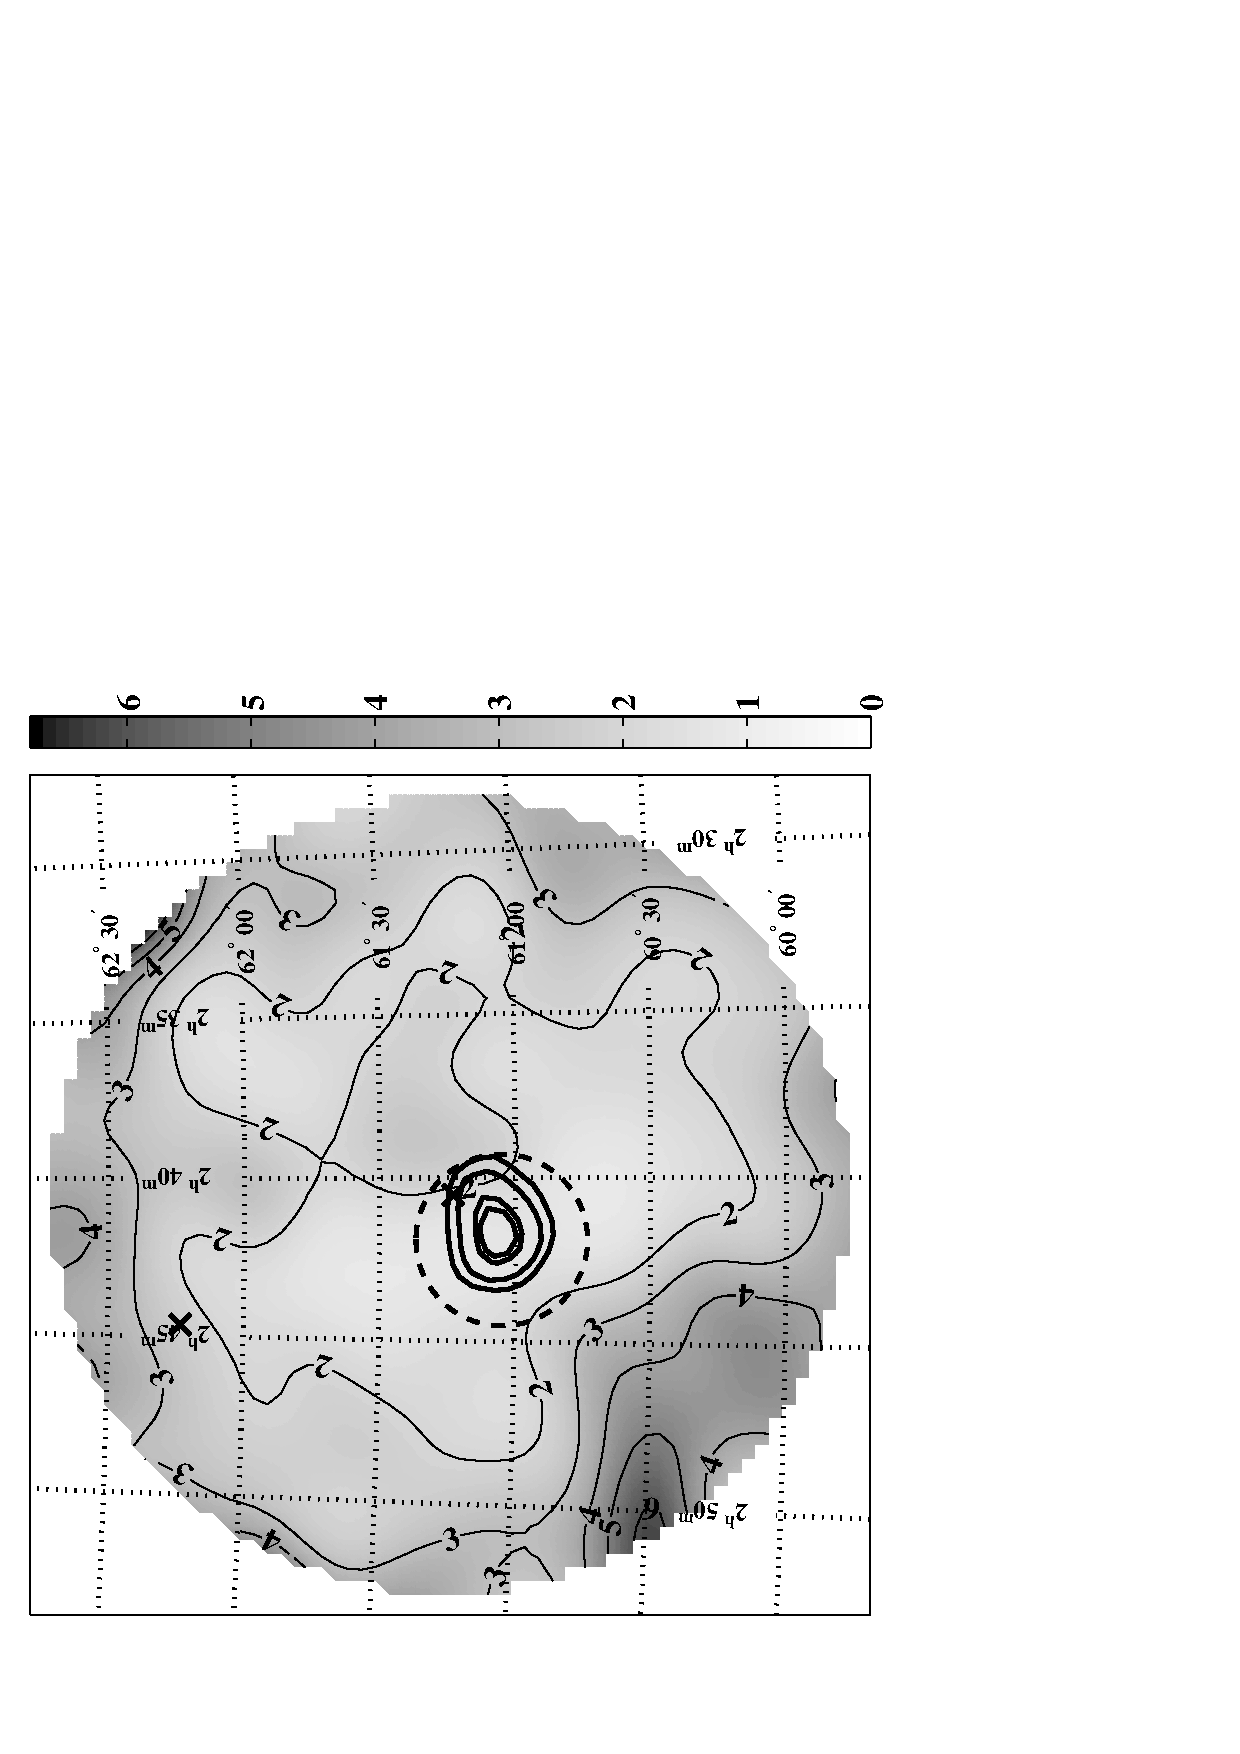
\includegraphics[draft=false,width=\textwidth,angle=270]{plots/chap-observations/loenergy/J0241+6103_sul_conv_bw.pdf}\includegraphics[width=\textwidth,angle=270]{plots/chap-observations/spectra/3EG_J0241+6103.pdf}}
\caption{\label{FIG::OBSERVATIONS::J0241} (Left) Limits on emission from 
3EG J0241$+$6103 in units of $10^{-11}$\,cm$^{-2}$\,s$^{-1}$. The 3EG
error contours are overlaid as heavy lines, the GeV catalog contour is
shown as a broken circle. (right) Spectrum from the on-line version of the 3EG
catalog with upper limit at 350\,GeV. The limit at 500\,GeV from 
\citet{REF::HALL::APJ2003} is also indicated.}
\end{figure}

The 3EG source has a spectral index of $\Gamma=2.21$, a large 100\,MeV
flux and shows evidence of variability. \citet{REF::KNIFFEN::APJ1997}
show that the variations in the \Gray flux are not correlated with the
radio outbursts. An exposure of 524\,min.\ was taken with the Whipple
telescope between November 2000 and February 2001, centered on the
binary system, offset by $\sim$0.25$^\circ$ from the center of the 3EG
source. No significant emission is detected and an upper limit of
$F_{(>350\,\mathrm{GeV})}<2.2\times10^{-11}$\,cm$^{-2}$\,s$^{-1}$ is
derived for emission withing the 3EG 95\%
contour. Figure~\ref{FIG::OBSERVATIONS::J0241} shows a map of upper
limits of emission from the region with the location of
LSI~$+$61$^\circ$303 and QSO~4U0241$+$61 indicated with an ``X'' (near
the center and displaced by a degree to the north respectively). It is
evident from the figure that the binary system lies outside of the
95\% confidence contour of the EGRET data, although it does lie within
the considerably larger 95\% confidence circle from the GeV
catalog. As noted by
\citet{REF::ROBERTS::APJS2001} based on an image of the region with
the ASCA instrument, there are no good x-ray candidates within the
95\% confidence contour for this
source. Table~\ref{TAB::OBSERVATIONS::J0241} shows the upper limits
derived for these candidate sources.

\begin{table}[t]
\caption{\label{TAB::OBSERVATIONS::J0241} Upper limits for candidates
in 3EG~J0241$+$6103 field.}
\centerline{\begin{tabular}{lllll}\hline
Source Name & \multicolumn{2}{l}{Coordinates} & Extent & Upper Limit \\
& $\alpha_{2000}$ & $\delta_{2000}$ & deg & $\times10^{-11}$\,cm$^{-2}$\,s$^{-1}$\\\hline
3EG~J0241$+$6103     & $02^h41^m31.3^s$ & $+61^\circ04^{\prime}12.3^{\prime\prime}$ & 0.21$\times$0.15 & 2.2 \\
LSI~$+$61$^\circ$303 & $02^h40^m31.4^s$ & $+61^\circ13^{\prime}45.6^{\prime\prime}$ & -                & 1.7 \\
QSO~4U0241$+$61      & $02^h44^m37.3^s$ & $+62^\circ13^{\prime}57.0^{\prime\prime}$ & -                & 2.3 \\\hline
\end{tabular}}
\end{table}

LSI~$+$61$^\circ$303 was previously observed with the Whipple
telescope between 1996 and 1999, with no significant excess of \Grays
being observed; a limit of
$F_{(>500\,\mathrm{GeV})}<0.88\times10^{-11}$\,cm$^{-2}$\,s$^{-1}$ was
reported by \citet{REF::HALL::APJ2003}. Assuming that the 3EG source
corresponds to the LSI~$+$61$^\circ$303, this paper shows that an
exponential cutoff is required in the extrapolated EGRET spectrum to
accommodate the VHE observations. Almost all of the flux phase space
at 350\,GeV allowed by extrapolating the EGRET spectrum is ruled out
by the upper limit reported here. After a quarter century of study,
2CG~135$+$01 remains one of the most puzzling of all \Gray
sources.

\subsection{3EG~J0423$+$1707}

3EG~J0423$+$1707 is an EGRET source about which very little is known at
other wavelengths. The 3EG error circle is large, at
$0.88^\circ\times0.65^\circ$, and it has the softest spectrum among
all of the sources chosen for this
survey. \citet{REF::MATTOX::APJS2001} suggest the radio source
B0422$+$1749 as a possible, but unlikely, counterpart, with a
probability of $2\times10^{-4}$.

\begin{figure}[t]
\resizebox*{\textwidth}{!}{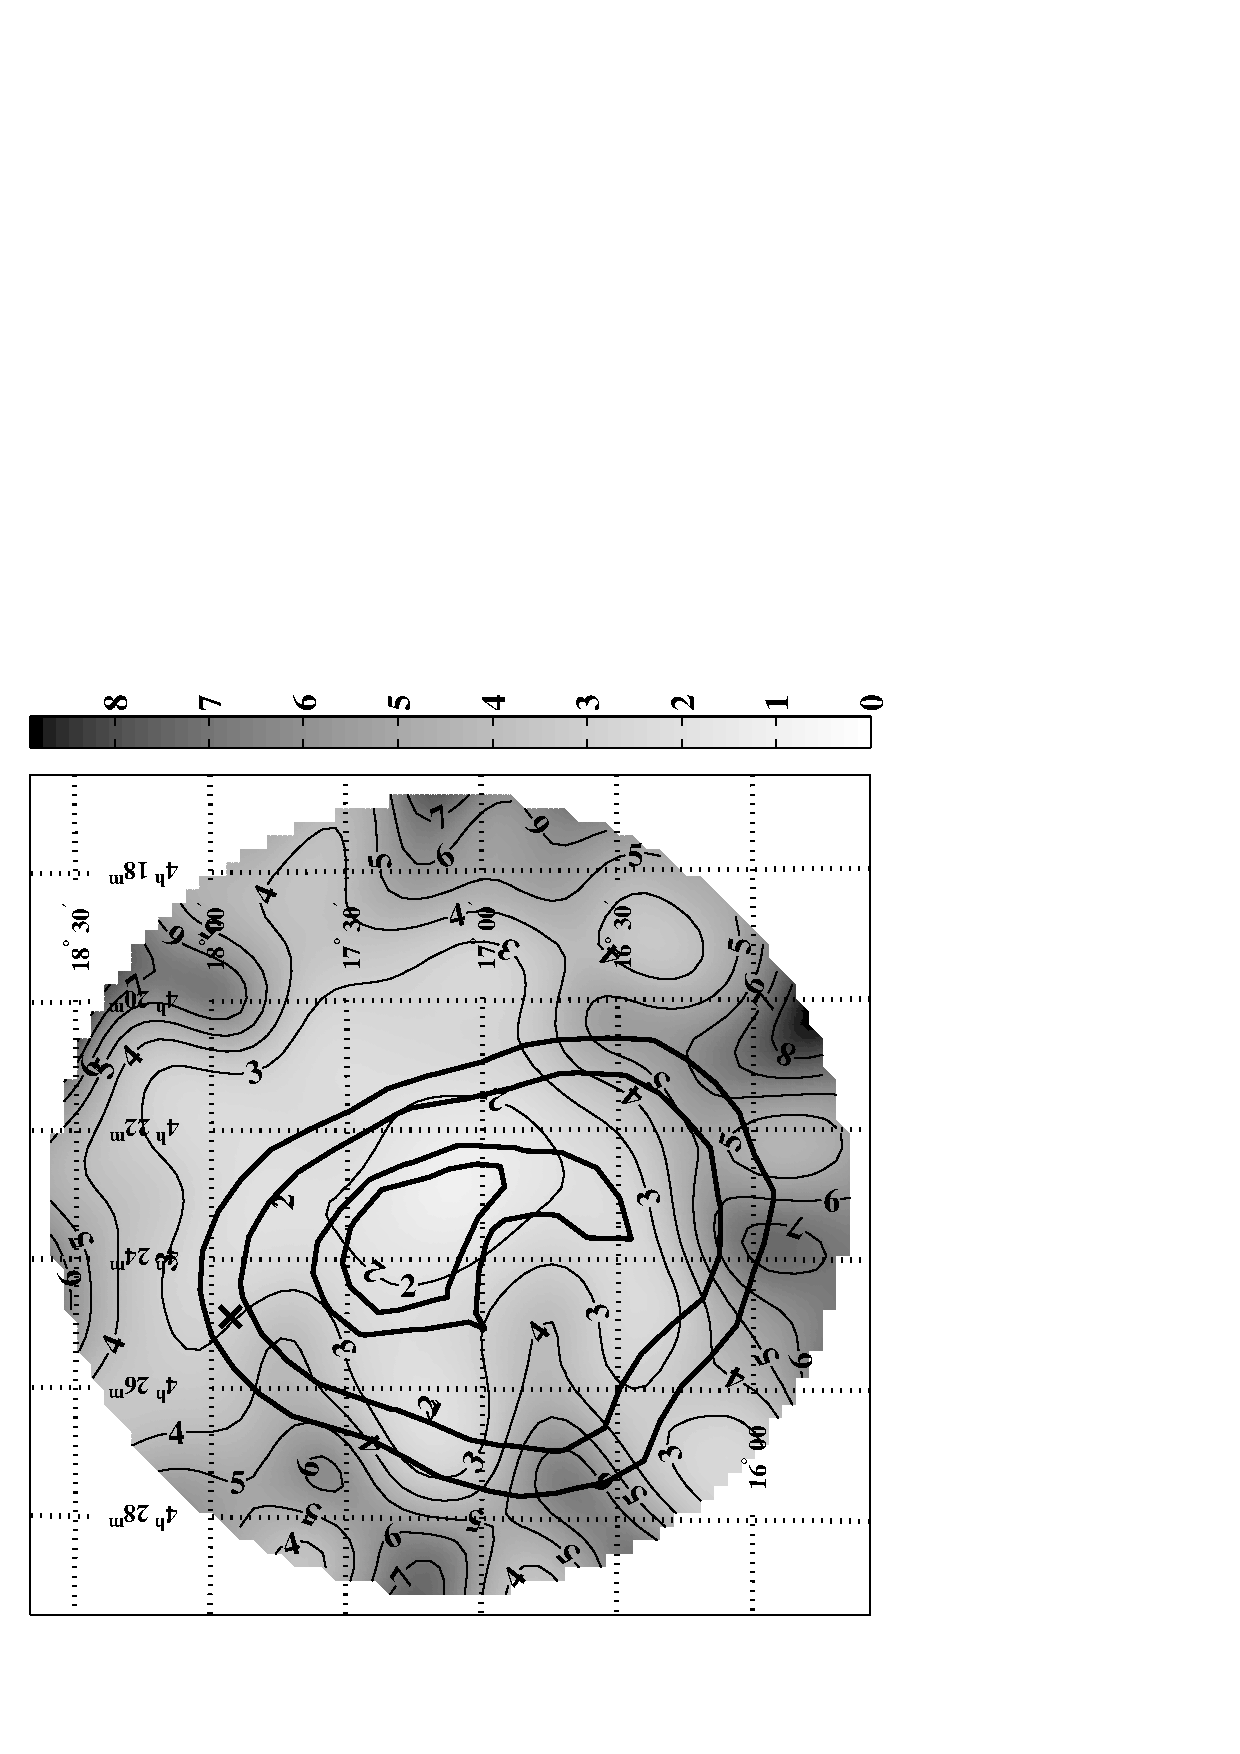
\includegraphics[draft=false,width=\textwidth,angle=270]{plots/chap-observations/loenergy/J0423+1707_sul_conv_bw.pdf}\includegraphics[width=\textwidth,angle=270]{plots/chap-observations/spectra/3EG_J0423+1707.pdf}}
\caption{\label{FIG::OBSERVATIONS::J0423} (Left) Limits on emission from 
3EG J0423$+$1707 in units of $10^{-11}$\,cm$^{-2}$\,s$^{-1}$. The 3EG
error contours are overlaid as heavy lines. (Right) Spectrum from the
on-line version of 3EG catalog with the upper limit at 350\,GeV.}
\end{figure}

\begin{table}[t]
\caption{\label{TAB::OBSERVATIONS::J0423} Upper limits for candidates
in 3EG~J0423$+$1707 field.}
\centerline{\begin{tabular}{lllll}\hline
Source Name & \multicolumn{2}{l}{Coordinates} & Extent & Upper Limit \\
& $\alpha_{2000}$ & $\delta_{2000}$ & deg & $\times10^{-11}$\,cm$^{-2}$\,s$^{-1}$\\\hline
3EG~J0423$+$1707     & $04^h23^m56.5^s$ & $+16^\circ56^{\prime}27.4^{\prime\prime}$ & 0.88$\times$0.65 & 6.6 \\
B0422$+$1749         & $04^h24^m53.4^s$ & $+17^\circ55^{\prime}49.9^{\prime\prime}$ & -                & 2.8 \\\hline
\end{tabular}}
\end{table}

The VHE observation consists of 193\,min.\ of data pointed at the center
of the 3EG source. No significant emission is observed, and an upper
limit of $F_{(>350\,\mathrm{GeV})}<6.6\times10^{-11}$\,cm$^{-2}$\,s$^{-1}$ is
derived for VHE emission within the 95\% confidence contour. A limit
of $F_{(>350\,\mathrm{GeV})}<2.8\times10^{-11}$\,cm$^{-2}$\,s$^{-1}$ applies to
the radio source B0422$+$1749. As is clear from
figure~\ref{FIG::OBSERVATIONS::J0423}, this limit does not constrain
the extrapolated EGRET spectrum.


\subsection{GeV~J0433$+$2907}

The \Gray source 3EG~J0433$+$2908 is listed as possibly being
associated with the radio source 87GB~0430$+$2859 in the 3EG catalog,
and was assumed to be an AGN. The \Gray source is unusual for an EGRET
AGN; the spectrum is particularly hard with no indication of a break
at energies up to 10\,GeV. \citet{REF::DINGUS::GAMMA2001}, analyzed
all of the EGRET photons at energies above 10\,GeV and show that three
are consistent with having originated from the location of the radio
source. At these energies the EGRET point-spread function is
considerably better than at 100\,MeV; given this improved PSF, they
calculate a probability of $1.9\times10^{-6}$ that three photons could
be associated with the source location purely by chance.
\citet{REF::WALLACE::GAMMA2001} gather together  compelling evidence 
that the radio source corresponds to an AGN: optical observations show
a featureless optical spectrum typical of a BL~Lac and the spectral
energy distribution\footnote{An SED, or $\nu F_\nu$ plot, for an
object is a graphical representation of the power an instrument would
receive across the spectrum given the assumption that its bandwidth is
proportional to the frequency. SEDs are usually displayed in units of
Ja\,Hz, W\,m$^{-2}$ or erg\,cm$^{-2}$\,s$^{-1}$ and are equivalent to
the E$^2$\,dF/dE plots presented in this chapter.}, or SED, shows a
clear two-peaked distribution, indicating synchrotron/inverse-Compton
(IC) emission that is typical for AGN. Assuming that the \Gray source
corresponds to the radio/x-ray source, the SED for 3EG~J0433$+$2908 is
shown in figure~\ref{FIG::OBSERVATIONS::SED0433}, and will be
discussed further below. No successful redshift measurements have been
made for this object, \citet{REF::HALPERN::AJ2003} report on repeated
attempts to determine the redshift and argue that $z>0.3$ for this object.

\begin{figure}[p]
\resizebox*{\textwidth}{!}{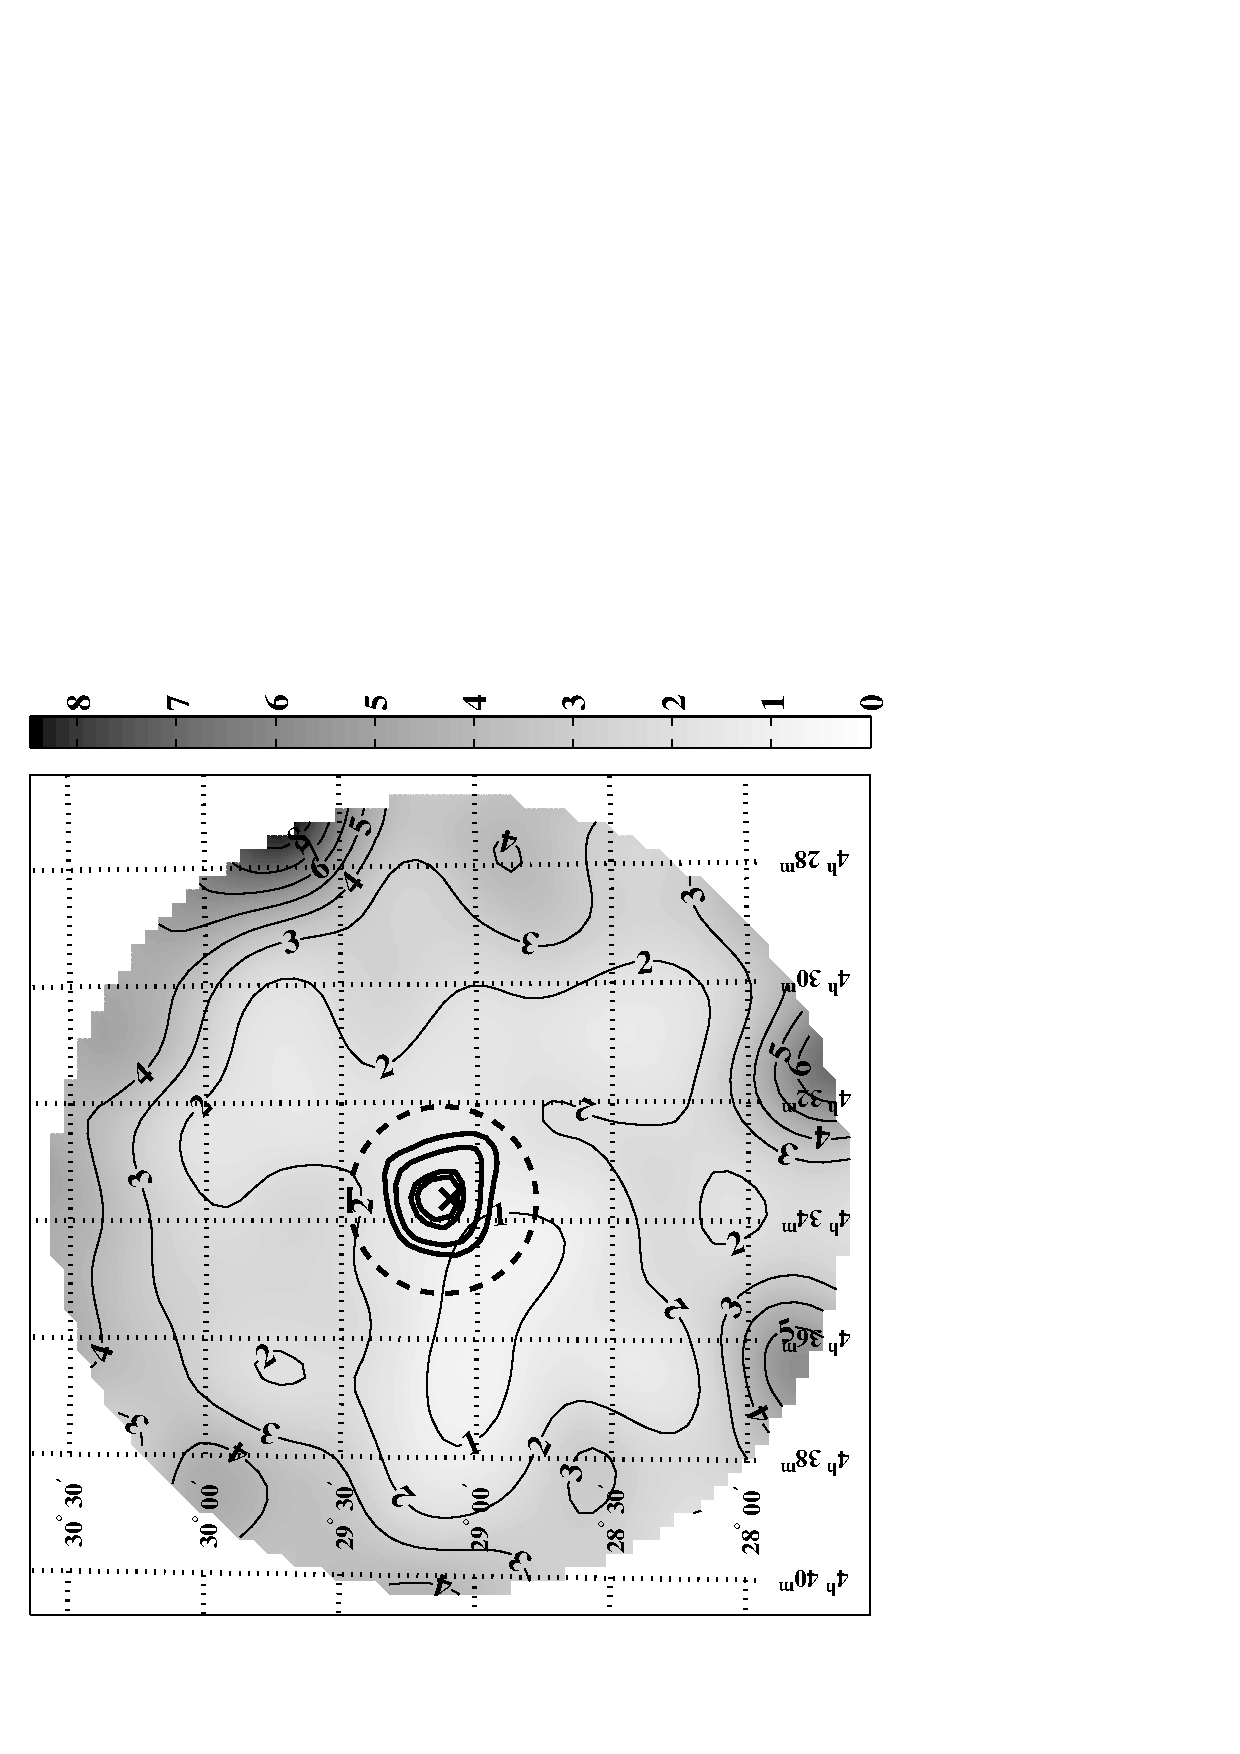
\includegraphics[draft=false,width=\textwidth,angle=270]{plots/chap-observations/loenergy/J0433+2908_sul_conv_bw.pdf}\includegraphics[width=\textwidth,angle=270]{plots/chap-observations/spectra/3EG_J0433+2908.pdf}}
\caption{\label{FIG::OBSERVATIONS::J0433} (Left) Limits on 
emission from 3EG J0433$+$2908 in units of
$10^{-11}$\,cm$^{-2}$\,s$^{-1}$. The 3EG error contours are overlaid
as heavy lines, the GeV catalog contour is shown as a broken
circle. (Right) Spectrum from the on-line version of the 3EG catalog with
the upper limit at 350\,GeV.}
\end{figure}

Between November 1999 and January 2002 a total of 1900\,min.\ of data
were taken with the Whipple instrument pointed at the GeV catalog
source location, which is coincident with the radio/x-ray source.
Prior to the publication of \citet{REF::DINGUS::GAMMA2001}, 500\,min.\
of data were collected in the \On/\Off\ mode, suitable for analysis
using the two-dimensional reconstruction technique. No significant
emission was detected; figure~\ref{FIG::OBSERVATIONS::J0433} shows the
upper limits of emission that can be derived from these data. The
upper limit within the 3EG 95\% error contour is
$F_{(>350\,\mathrm{GeV})}<1.6\times10^{-11}$\,cm$^{-2}$\,s$^{-1}$. This
limit is displayed with the 3EG spectrum in
figure~\ref{FIG::OBSERVATIONS::J0433}. To reconcile the limit with the
increasing EGRET spectrum a cut-off in the spectrum at an energy
greater than 10\,GeV is required. The remainder of the VHE data was
taken in the \Trk\ mode, and is not suitable for 2D analysis but can
provide a more sensitive limit on emission from the radio/x-ray
source. A limit of
$F_{(>350\,\mathrm{GeV})}<0.76\times10^{-11}$\,cm$^{-2}$\,s$^{-1}$ is
derived from all of the data combined. This limit is shown on a SED
for the object in figure~\ref{FIG::OBSERVATIONS::SED0433}. It must be
noted that the distribution was produced with
\textit{non-contemporaneous} data; since the SED of an AGN can change
considerably as the sources goes from a quiescent to a flaring state,
figure~\ref{FIG::OBSERVATIONS::SED0433} should be considered as
approximate. The double peaked structure is clearly visible, with the
peak in the synchrotron emission occurring somewhere in the optical to
x-ray band and the peak in the IC emission occurring between the HE
and VHE \Gray regimes.

\begin{table}[t]
\caption{\label{TAB::OBSERVATIONS::J0433} Upper limits for candidates
in 3EG~J0433$+$2908 field.}
\centerline{\begin{tabular}{lllll}\hline
Source Name & \multicolumn{2}{l}{Coordinates} & Extent & Upper Limit \\
& $\alpha_{2000}$ & $\delta_{2000}$ & deg & $\times10^{-11}$\,cm$^{-2}$\,s$^{-1}$\\\hline
3EG~J0433$+$2908     & $04^h33^m35.1^s$ & $+29^\circ07^{\prime}42.2^{\prime\prime}$ & 0.19$\times$0.16 & 1.6 \\
87GB~0430$+$2859     & $04^h33^m37.5^s$ & $+29^\circ05^{\prime}53.0^{\prime\prime}$ & -                & 0.8 \\\hline
\end{tabular}}
\end{table}

\begin{figure}[p]
\centerline{\includegraphics[angle=270,width=0.8\textwidth]{plots/chap-observations/sed0433.pdf}}
\caption{\label{FIG::OBSERVATIONS::SED0433} Spectral energy 
distribution for the radio/x-ray source RX~J0433.5$+$2906. The radio data
come from the NASA/IPAC extragalactic database (NED). The IR
observations are from the 2 micron all sky survey (2MASS). Optical
data are from \citet{REF::HALPERN::AJ2003}. The x-ray flux is from the
ROSAT all sky survey bright source catalog (RASS-BSC). Finally, the 
differential \Gray flux is from the on-line 3EG catalog.}
\end{figure}

\enlargethispage{12pt} Typically, for a low-frequency peaked BL~Lac 
(LBL) the peak in the synchrotron emission occurs in the far-infrared
to optical bands, with the IC peak below 100\,MeV, so that the
emission is falling through the EGRET energy range. Conversely, for an
HBL (high frequency peaked BL~Lac) the peak in the synchrotron
emission occurs at UV to soft x-ray energies. The IC component then
peaks at GeV to TeV energies. The SED for this object resembles most
that of an HBL. The object seems to be intermediate between the
typical EGRET BL~Lac and the VHE selected extreme HBLs. It is
reasonable to conclude that a cutoff is required between 10\,GeV and
$\sim100$\,GeV, either due to a feature intrinsic to the source
spectrum or due to absorption of the \Gray signal in the
extra-galactic background light, especially if the object is at a
distance of $z>0.3$. On the other hand, it is also possible that the
state of the object was different when the various observations were
made, i.e.\ flaring when EGRET observed it and quiescent during the
VHE observations, in which case a cutoff may not be required. However,
since the EGRET spectrum represents a mean spectrum over all viewing
periods, this is unlikely.

\subsection{3EG~J0450$+$1105}

With a spectral index of 2.27, 3EG~J0450$+$1105 has one of the softer
spectra of the sources chosen in this survey. The source is not
detected as a significant source in the GeV catalog, although it is
listed as a ``source of GeV gamma rays based upon the search for
repeating, weak outbursts'' in the second part of the catalog
\citep{REF::MACOMB::ICRC1999}. The source is consistent with being 
highly variable: it has a variability index of 1.13 and its flux is
listed in the 3EG catalog as having a maximum of
$109.5\times10^{-8}$\,cm$^{-2}$\,s$^{-1}$ during EGRET viewing period
\#36 while its average flux over all viewing periods is
$14.9\times10^{-8}$\,cm$^{-2}$\,s$^{-1}$.

\citet{REF::MATTOX::APJS2001} suggest that the \Gray source is
associated with the radio source B0446$+$1116, an AGN, with a
probability level of 0.14. \citet{REF::HALPERN::AJ2003} confirm this
association, and present their attempts to resolve a redshift for the
object. They claim that the accepted redshift of $z=1.207$ is likely
incorrect, and that the featureless spectrum they obtained makes it
impossible to derive an unambiguous redshift. Depending on how the
minor features in the spectrum are interpreted, they suggest $z=0.74$
or $z=0.21$ as possible values, with the lower value being less
likely.

\begin{figure}[p]
\resizebox*{\textwidth}{!}{\includegraphics[draft=false,width=\textwidth,angle=270]{plots/chap-observations/loenergy/J0450+1105_sul_conv_bw.pdf}\includegraphics[width=\textwidth,angle=270]{plots/chap-observations/spectra/3EG_J0450+1105.pdf}}
\caption{\label{FIG::OBSERVATIONS::J0450} (Left) Limits on 
emission from 3EG~J0450$+$1105 in units of
$10^{-11}$\,cm$^{-2}$\,s$^{-1}$. The 3EG error contours are overlaid
as heavy lines. (Right) Spectrum from the on-line version of the 3EG
catalog with the limit at 350\,GeV.}
\end{figure}

\begin{figure}[p]
\centerline{\includegraphics[angle=270,width=0.8\textwidth]{plots/chap-observations/sed0450.pdf}}
\caption{\label{FIG::OBSERVATIONS::SED0450} Spectral energy 
distribution for the radio/x-ray source PKS~B0446$+$112. The data are from
the same sources as in figure~\ref{FIG::OBSERVATIONS::SED0433}.  The
x-ray source (1RXS~J044903.0$+$112120) was not strong enough to be
included in the the RASS-BSC, the x-ray flux was estimated from the
count rate in the RASS catalog, and should be considered as
approximate.}
\end{figure}

A total of 264\,min.\ of VHE observations were made between November
2000 and February 2001. No significant excess was seen, although there
was a $3\sigma$ deficit of events at one location. Given the large
number of fields viewed in this survey, a $3\sigma$ deficit (or
excess) is not statistically significant, see
figure~\ref{FIG::ANALYSIS::SIGMASIGMA}.  The upper limits derived from
the observations are shown in figure~\ref{FIG::OBSERVATIONS::J0450}
and summarized in table~\ref{TAB::OBSERVATIONS::J0450}. The limit for
emission within the large EGRET error-box is
$F_{(>350\,\mathrm{GeV})}<5.0\times10^{-11}$\,cm$^{-2}$\,s$^{-1}$.

Figure~\ref{FIG::OBSERVATIONS::SED0450} shows an SED for the radio
source obtained from published data. The source was only weakly
detected by ROSAT, it is absent from the ROSAT bright source catalog
(RASS-BSC) but is present in the electronic version of the ROSAT all
sky survey (RASS). The SED clearly shows the two peaked structure,
typical of an LBL, with the synchrotron emission peaking in the
IR-optical band and the IC component peaking below 100\,MeV. The upper
limit derived for the location of the radio source is also shown; it
is clear from the figure that, due to the soft spectrum, the VHE upper
limit does not constrain the emission significantly.

\begin{table}[t]
\caption{\label{TAB::OBSERVATIONS::J0450} Upper limits for candidates
in 3EG~J0450$+$1105 field.}
\centerline{\begin{tabular}{lllll}\hline
Source Name & \multicolumn{2}{l}{Coordinates} & Extent & Upper Limit \\
& $\alpha_{2000}$ & $\delta_{2000}$ & deg & $\times10^{-11}$\,cm$^{-2}$\,s$^{-1}$\\\hline
3EG~J0450$+$1105  & $22^h15^m06.5^s$ & $+31^\circ28^{\prime}55.7^{\prime\prime}$ & 0.65$\times$0.61 & 5.0 \\
B0446$+$1116      & $04^h49^m07.7^s$ & $+11^\circ21^{\prime}28.6^{\prime\prime}$ & -                & 1.3 \\\hline
\end{tabular}}
\end{table}

\subsection{GeV~J0508$+$0540}

The \Gray source GeV~J0508$+$0540 is listed in the GeV catalog as a
``low-significance source'', with $23\pm7$ photons detected from the
source at E$>$1\,GeV. It was not seen significantly at 100\,MeV, and
consequently had no corresponding 3EG
entry. \citet{REF::DINGUS::GAMMA2001} list two EGRET photons with
energies greater than 40\,GeV from the object. The two photons are
consistent with having originated from the BL~Lac 0509$+$056, to
within 4\,arcmin, with probability of $1.3\times10^{-8}$ of occurring
by chance. \citet{REF::HALPERN::AJ2003} report several unsuccessful
attempts to measure the redshift of this object; the optical spectra
they recorded were featureless and no host galaxy could be resolved.

The VHE observations of this source consist of 842\,min.\ of data
taken between October and December 2001, pointing at the radio/x-ray
source. The data were recorded in the \Trk\ mode, under the assumption
that the \Gray source was the AGN, and are unsuitable for analysis
with the two-dimensional method. For this source alone, no source maps
are presented. No significant excess was observed, the limit on
emission from the AGN is
$F_{(>350\,\mathrm{GeV})}<0.73\times10^{-11}$\,cm$^{-2}$\,s$^{-1}$.

An approximate SED for this object is presented in figure
\ref{FIG::OBSERVATIONS::SED0508}. Since no 3EG detection was achieved, a
differential spectrum is not available for this source; an upper limit
at 100\,MeV and the integral flux from the GeV catalog, transformed
into a differential flux assuming a differential power-law spectrum of
index 2.0\footnote{The spectrum is probably harder than 2.0 so the
fluxes may be a little \textit{higher} than plotted.}, are
displayed. No flux at $>$10\,GeV is listed in
\citet{REF::DINGUS::GAMMA2001}, due to the small number of photons
detected and a lack of understanding of the performance of
anti-coincidence shield at these energies. A preliminary flux was
obtained from the author
\citep{REF::DINGUS::PRIVATE2001} and is plotted in
figure~\ref{FIG::OBSERVATIONS::SED0508}.

\begin{figure}[t]
\centerline{\includegraphics[angle=270,width=0.8\textwidth]{plots/chap-observations/sed0508.pdf}}
\caption{\label{FIG::OBSERVATIONS::SED0508} Spectral energy 
distribution for the radio/x-ray source RX~J0509.3$+$0541. The data
come from the same sources as in
figure~\ref{FIG::OBSERVATIONS::SED0433} with the 100\,MeV upper limit
from \citet{REF::HARTMAN::APJS1999} (see
figure~\ref{FIG::INTRODUCTION::3RDEGRETUL}), the 1\,GeV \Gray flux
from \citet{REF::LAMB::APJ1997}, and the preliminary 10\,GeV point
from \citet{REF::DINGUS::PRIVATE2001}.}
\end{figure}

\begin{table}[t]
\caption{\label{TAB::OBSERVATIONS::J0508} Upper limits for RX~J0509.3$+$0541.}
\centerline{\begin{tabular}{lllll}\hline
Source Name & \multicolumn{2}{l}{Coordinates} & Extent & Upper Limit \\
& $\alpha_{2000}$ & $\delta_{2000}$ & deg & $\times10^{-11}$\,cm$^{-2}$\,s$^{-1}$\\\hline
RX~J0509.3$+$0541        & $05^h09^m26.0^s$ & $+05^\circ41^{\prime}35.4^{\prime\prime}$ & - & 0.73 \\\hline
\end{tabular}}
\end{table}

EGRET did not resolve the peak in the high energy component of the
emission below 10\,GeV, suggesting that the object resembles an HBL.
There is insufficient data at lower energies to resolve the peak in
the low energy component; it is possible that the synchrotron emission
peaks at or below the IR/optical points in the SED, in which case the
x-ray emission results from IC up-scattering. Alternatively, the low
energy emission may peak between the optical and x-ray energies with
the x-rays resulting from synchrotron emission. Although it is not
possible to definitely rule out either scenario, usual SSC models
would have difficulty in explaining the \Gray emission (both lack of
100\,MeV emission and increasing emission through 10\,GeV) in the
former case. It was the fact that, like many VHE selected HBLs, the
source was not seen in the 3EG catalog that initially suggested that
this source would be an interesting one to study in the VHE
regime. Based on the preliminary 10\,GeV point, a strong cutoff in the
emission is required to accommodate the VHE upper limit. The cutoff
may be from absorption in the extragalactic background light if the
source is at a large redshift, or may be intrinsic to the source
spectrum.

\subsection{3EG~J0613$+$4201}

3EG~J0613$+$4201 is a 100\,MeV and 1\,GeV \Gray source at mid-Galactic
latitude with a relatively hard spectrum, weak flux, large error-box
and a high variability index. \citet{REF::MATTOX::APJS2001} list three
possible radio counterparts for the source, all outside of the 95\%
3EG contour. None of the potential associations are very compelling,
in each case the probability of the association being correct is
listed as $\le10^{-4}$.

\begin{table}[b]
\caption{\label{TAB::OBSERVATIONS::J0613} Upper limits for candidates
in 3EG~J0613$+$4201 field.}
\centerline{\begin{tabular}{lllll}\hline
Source Name & \multicolumn{2}{l}{Coordinates} & Extent & Upper Limit \\
& $\alpha_{2000}$ & $\delta_{2000}$ & deg & $\times10^{-11}$\,cm$^{-2}$\,s$^{-1}$\\\hline
3EG~J0613$+$4201 & $06^h14^m20.6^s$ & $+41^\circ59^{\prime}51^{\prime\prime}$ & 0.66$\times$0.46 & 4.3 \\
87GB~0609$+$4123 & $06^h12^m51.2^s$ & $+41^\circ22^{\prime}37^{\prime\prime}$ & -                & 1.9 \\
87GB~0612$+$4131 & $06^h16^m22.4^s$ & $+41^\circ30^{\prime}48^{\prime\prime}$ & -                & 3.1 \\
87GB~0614$+$4209 & $06^h18^m08.6^s$ & $+41^\circ08^{\prime}00^{\prime\prime}$ & -                & 2.9 \\\hline
\end{tabular}}
\end{table}

\begin{figure}[t]
\resizebox*{\textwidth}{!}{\includegraphics[draft=false,width=\textwidth,angle=270]{plots/chap-observations/loenergy/J0613+4201_sul_conv_bw.pdf}\includegraphics[width=\textwidth,angle=270]{plots/chap-observations/spectra/3EG_J0613+4201.pdf}}
\caption{\label{FIG::OBSERVATIONS::J0613} (Left) Limits on 
emission from 3EG J0613$+$4201 in units of
$10^{-11}$\,cm$^{-2}$\,s$^{-1}$. The 3EG error contours are overlaid
as heavy lines, the GeV catalog contour is shown as a broken
circle. (Right) Spectrum from the on-line version of the 3EG catalog with
the upper limit at 350\,GeV.}
\end{figure}

The VHE observations of this source, which were made over two
observing seasons, between November 2001 and January 2003, consist of
275\,min.\ of data taken pointed at the center of the 3EG source. No
significant emission was detected and a limit of
$F_{(>350\,\mathrm{GeV})}<4.3\times10^{-11}$\,cm$^{-2}$\,s$^{-1}$ is
placed on emission from within the 95\% confidence contour. Upper
limits for the region are presented in
figure~\ref{FIG::OBSERVATIONS::J0613}, with the locations of the three
potential candidates marked. The limits derived for these locations
are presented in table~\ref{TAB::OBSERVATIONS::J0613}. The limit is
not sensitive enough to rule out a simple extrapolation of the EGRET
spectrum into the VHE regime.


\subsection{3EG~J0628$+$1847}

\begin{figure}[p]
\resizebox*{\textwidth}{!}{\includegraphics[draft=false,width=\textwidth,angle=270]{plots/chap-observations/loenergy/J0628+1847_sul_conv_bw.pdf}\includegraphics[width=\textwidth,angle=270]{plots/chap-observations/spectra/3EG_J0628+1847.pdf}}
\caption{\label{FIG::OBSERVATIONS::J0628} (Left) Limits on 
emission from 3EG J0628$+$1847 in units of
$10^{-11}$\,cm$^{-2}$\,s$^{-1}$. The 3EG error contours are overlaid
as heavy lines. (Right) Spectrum from the on-line version of the 3EG
catalog with the limit at 350\,GeV.}
\end{figure}

\begin{figure}[p]
\centerline{\includegraphics[angle=270,width=0.8\textwidth]{plots/chap-observations/sed0628.pdf}}
\caption{\label{FIG::OBSERVATIONS::SED0628} Spectral energy 
distribution for the radio/x-ray source RX~J0631.4$+$1908
(87GB~0628$+$1911), assuming it is associated with the \Gray
source. The data come from the same sources as in
figure~\ref{FIG::OBSERVATIONS::SED0433}.}
\end{figure}

The \Gray source 3EG~J0628$+$1847 has a relatively weak spectral
index, an average 100\,MeV flux and lies at a low Galactic
latitude. Its variability index could not be determined by
\citet{REF::NOLAN::APJ2003}, since the source failed a consistency
check during their analysis. Despite being close to the Galactic
plane, \citet{REF::ROMERO::AA1999} report no positional associations
with known SNR, OB associations or WR- and O-type
stars. \citet{REF::MATTOX::APJS2001} list two radio sources from the
Green Bank catalog in the field, one just inside the 95\% confidence
contour, the other just inside the 99\% contour; these are listed as
having probabilities of $2\times10^{-4}$ and $9\times10^{-4}$,
respectively, of being counterparts. The second radio source,
87GB~0628$+$1971, is listed as coincident with a ROSAT x-ray source by
\citet{REF::LAURENT_MUEHLEISEN::AAS1997} and has an associated IR 
point source in the 2MASS catalog.

VHE observations of the 3EG source were made between December 2001 and
February 2003. A total of 331\,min.\ of usable data were collected and
analyzed using the two-dimensional technique. No significant emission
was seen in the field; the upper limits on emission that are derived
from the data are presented in figure~\ref{FIG::OBSERVATIONS::J0628}.
The upper limit from within the 95\% error contour is
$F_{(>350\,\mathrm{GeV})}<4.1\times10^{-11}$\,cm$^{-2}$\,s$^{-1}$, and is
displayed with the EGRET spectrum on the right hand side of
figure~\ref{FIG::OBSERVATIONS::J0628}. The VHE upper limit does
not constrain an extrapolation of the EGRET spectrum to 350\,GeV.

The upper limits for the two candidates from
\citet{REF::MATTOX::APJS2001}, are presented in
table~\ref{TAB::OBSERVATIONS::J0628}. Assuming that the
\Gray source is associated with 87GB~0628$+$1911, an approximate SED for the
object is shown in figure~\ref{FIG::OBSERVATIONS::SED0628}. The
distribution shows a bimodal structure, typical of an AGN. Since the
HE component peaks somewhere below 100\,MeV, the source is likely an
LBL. The VHE limit appropriate to the source location does not
significantly constrain the spectrum above 10\,GeV.

\begin{table}[t]
\caption{\label{TAB::OBSERVATIONS::J0628} Upper limits for candidates
in 3EG~J0628$+$1847 field.}
\centerline{\begin{tabular}{lllll}\hline
Source Name & \multicolumn{2}{l}{Coordinates} & Extent & Upper Limit \\
& $\alpha_{2000}$ & $\delta_{2000}$ & deg & $\times10^{-11}$\,cm$^{-2}$\,s$^{-1}$\\\hline
3EG~J0628$+$1847 & $06^h28^m36.1^s$ & $+18^\circ50^{\prime}35^{\prime\prime}$ & 0.66$\times$0.49 & 4.1 \\
87GB~0624$+$1833 & $06^h27^m20.5^s$ & $+18^\circ31^{\prime}04^{\prime\prime}$ & -                & 1.5 \\
87GB~0628$+$1911 & $06^h31^m32.3^s$ & $+19^\circ08^{\prime}41^{\prime\prime}$ & -                & 2.6 \\\hline
\end{tabular}}
\end{table}

\subsection{3EG~J0634$+$0521 and 3EG~J0631$+$0642}

The \Gray sources J0634$+$0521 and J0631$+$0642 both lie in the region of
the Monoceros supernova remnant, although neither is explicitly associated
with it in the 3EG catalog. In addition, the GeV source J0633$+$0645
partially overlaps 3EG~J0631$+$0642 and is listed as a possible
counterpart to the SNR in \citet{REF::LAMB::APJ1997}.

The large shell-type SNR G205.5$+$0.5, or Monoceros Loop Nebula, is 220
arcmin in diameter, the fifth largest SNR in
\citet{REF::GREEN::WEB2001}. The SNR is thought to be
1.39$\pm$0.1\,kpc distant, and approximately $3-20\times 10^4$\,yr in
age, i.e.\ in the Sedov expansion phase. Monoceros was first
recognized as a source of 100\,MeV \Grays by
\citet{REF::ESPOSITO::APJ1996}. \citet{REF::JAFFE::APJ1997} presented a
map of EGRET \Gray emission over a large area around the SNR, where
they found evidence for an extended emission feature in the direction
of the Rossette nebula. They suggest that, since \Gray emission was
not seen uniformly across the remnant, the \Grays are produced in a
region of enhanced shock acceleration at the interaction between the
remnant and the nebula. \citet{REF::KAARET::APJ1999} used the
Beppo-SAX narrow-field instruments to image the region around
J0634$+$0521 and discovered a point source with a hard spectrum,
SAX~J0635$+$0553. They report an optical counterpart, which is likely
a B-type companion star, and conclude that if the \Gray emission is
associated with the system (or a portion of it is), then it is a \Gray
emitting x-ray binary.  When the x-ray observations were subsequently
revisited, a 33.8\,ms\ pulsation was discovered
\citep{REF::KAARET::APJ2000}. In a recent study of all potential EGRET
SNR counterparts,
\citet{REF::TORRES::PR2003}, suggest that the source of the \Gray
emission is far from resolved. The fact that Beppo-SAX did not
discover extended emission from the region, as would be expected in a
shock acceleration scenario, suggests that the binary may be
responsible for the \Gray emission. On the other hand, no orbital
variations are seen in the \Gray signal, arguing against an origin in
the binary system.  Analysis of the pulsar energetics and accretion
rate further confuses the issue, see \citet{REF::TORRES::PR2003} for
review. \citet{REF::LUCARELLI::HEGR2001} report preliminary evidence
for VHE \Gray emission from the region with the HEGRA telescope
system\footnote{At a $5.7\sigma$ level for emission based on
120\,hrs.\ at $E>500$\,GeV from four $0.2^\circ\times0.2^\circ$ bins
in the region of the Rossette nebula.}. The VHE emission was extended
and was not coincidental with the Beppo-SAX source. No flux was
reported for the observations.

\citet{REF::TORRES::PR2003} suggest that 3EG~J0643$+$0521 might be a
composite source, with the Beppo-SAX source being responsible for a
portion of the EGRET \Gray flux and the bulk of the x-ray emission,
while interactions between the SNR and the Rossette nebula may
contribute to the 3EG flux and account for any VHE emission. They
predict that, if a composite source is responsible, a spectral break
should be detected between the EGRET and ground-based \Gray regimes. For
3EG~J0631$+$0642 a pure shock acceleration model is sufficient to
explain the 3EG flux.

\citet{REF::ROMERO::AA1999} studied potential positional associations
between 3EG sources and SNR, OB associations, WR-type and O-type
stars.  In addition to the Monoceros SNR, they report two O-type stars
and two OB associations in the region: from a catalog of O-type stars
\citep{REF::CRUZ-GONZALEZ::RMAA1974} HD46150 and HD46223 and
from a catalog of OB-associations \citep{REF::MELNIK::AL1995}
Mon~OB~2A and Mon~OB~1B\footnote{\citet{REF::ROMERO::AA1999} refer to
Mon~OB~2B which is not in the catalog. Mon~OB~1B is the correct source
association.}. Mon~OB~1B lies just outside of the region studied in
this work.

The VHE observations of this source consist of 248\,min.\ of data. In
order to accomodate the 95\% confidence contours of both 3EG sources
and the GeV source, the telescope was pointed close to the coordinates
listed for the Monoceros nebula in \citet{REF::GREEN::WEB2001},
approximately half way between the two 3EG sources. Although both
EGRET sources were in the field of view they lie toward the edge of
the camera, which is less sensitive to \Grays than the center.

No significant emission was detected in the field;
figure~\ref{FIG::OBSERVATIONS::J0634UL} presents the upper limits
derived from the observations. The figure shows the EGRET contours for
both sources, with 3EG~J0634$+$0521 toward the lower left. The GeV
source is indicated as a dashed circle overlapping 3EG~J0631$+$0642.
The dash-dotted circle towards the bottom of the figure indicates the
location of Mon~OB~2A, with the two O-type stars, each marked by an
``X'' within. Finally, the location of SAX~J0635$+$0533 is marked as
an ``X'' near the center of
3EG~J0634$+$0521. Table~\ref{TAB::OBSERVATIONS::J0634} summarizes the
upper limits derived for the EGRET error-boxes and for the various
candidate sources.

\begin{table}[t]
\caption{\label{TAB::OBSERVATIONS::J0634} Upper limits for candidates
in the fields of 3EG J0634$+$0521 and 3EG J0631$+$0642.}
\centerline{\begin{tabular}{lllll}\hline
Source Name & \multicolumn{2}{l}{Coordinates} & Extent & Upper Limit \\
& $\alpha_{2000}$ & $\delta_{2000}$ & deg & $\times10^{-11}$\,cm$^{-2}$\,s$^{-1}$\\\hline
3EG~J0634$+$0521 & $06^h34^m39.9^s$ & $+05^\circ28^{\prime}21^{\prime\prime}$ & $0.85\times0.50$ & 5.3 \\
3EG~J0631$+$0642 & $06^h31^m39.4^s$ & $+06^\circ41^{\prime}42^{\prime\prime}$ & $0.55\times0.39$ & 6.0 \\
GeV~J0633$+$0645 & $06^h33^m08.8^s$ & $+06^\circ45^{\prime}49^{\prime\prime}$ & $0.42\times0.42$ & 4.9 \\
SAX~J0635$+$0533 & $06^h35^m17.4^s$ & $+05^\circ33^{\prime}21^{\prime\prime}$ & -                & 2.0 \\
Mon~OB~2A        & $06^h32^m10.2^s$ & $+04^\circ50^{\prime}46^{\prime\prime}$ & $0.33\times0.47$ & 4.7 \\
HD46150          & $06^h30^m36.0^s$ & $+04^\circ57^{\prime}00^{\prime\prime}$ & -                & 3.1 \\
HD46223          & $06^h31^m00.0^s$ & $+04^\circ50^{\prime}00^{\prime\prime}$ & -                & 2.4 \\\hline
\end{tabular}}
\end{table}

\begin{figure}[p]
\centerline{\includegraphics[draft=false,angle=270,width=0.75\textwidth]{plots/chap-observations/loenergy/J0634+0521_sul_conv_bw.pdf}}
\caption{\label{FIG::OBSERVATIONS::J0634UL} Upper limits on emission 
from 3EG~J0634$+$0521, 3EG~J0631$+$0642 and GeV~J0633$+$0645 in units of
$10^{-11}$\,cm$^{-2}$\,s$^{-1}$. The 3EG error contours are overlaid
as heavy lines, the GeV error circle as a dashed line toward the top
of the diagram. The dash-dotted ellipse toward the bottom of the figure
indicates the OB association Mon~OB~2A.}
\end{figure}

\begin{figure}[p]
\includegraphics[angle=270,width=0.49\textwidth]{plots/chap-observations/spectra/3EG_J0634+0521.pdf}\hspace*{\fill}\includegraphics[angle=270,width=0.49\textwidth]{plots/chap-observations/spectra/3EG_J0631+0642.pdf}
\caption{\label{FIG::OBSERVATIONS::J0634SPEC} Spectrum for 
3EG~J0634$+$0521 (left) and 3EG~J0631$+$0642 (right) from on-line
version of the 3EG catalog with the upper limit at 350\,GeV. The limit
at 500\,GeV from \citet{REF::LESSARD::ICRC1999} is also indicated.}
\end{figure}

The extrapolated EGRET spectra for both sources are shown in
figure~\ref{FIG::OBSERVATIONS::J0634SPEC} with the upper limits at
350\,GeV. These observations do not require a break in the spectrum of
either source and cannot substantiate (or refute) the two component
model of \citet{REF::TORRES::PR2003}. Although the previous upper
limits derived from observations with the Whipple telescope
\citep{REF::LESSARD::ICRC1999} had a lower flux value, the
observations were made at higher energy, and do not constrain the
extrapolated EGRET spectrum any more than these observations. The
previous limits are shown on the figure at 500\,GeV, at approximately
the same level. This source is a prime candidate for observation with
the next generation of ground-based instruments, such as VERITAS,
which will have an order of magnitude increase in sensitivity over the
current generation, and will operate at at energies
$\sim100$\,GeV. These instruments will have the ability to accurately
reconstruct the origin of the {\Grayc}s, and will have the ability to
resolve the \Gray emission from unidentified EGRET sources such as
this one.

\subsection{3EG~J1009$+$4855}

In the 3EG catalog, J1009$+$4855 is listed as having a low flux and a
hard, but relatively ill defined, spectral
index. \citet{REF::NOLAN::APJ2003} present only an upper limit for the
variability index, not surprising given the low mean flux from the
source and that it was not seen at a particularly high flux state during
any of the EGRET viewing periods. The source is also listed in the GeV
catalog as a low significance source. Very little is known about this source
at other wavelengths, the EGRET catalog suggests a weak association
with the radio/x-ray source B1011+496, a known AGN at redshift of
$z=0.2$. \citet{REF::MATTOX::APJS2001} lists the probability of that
association as $2\times10^{-4}$; the radio-source lies outside of
the large 99\% error contour\footnote{The EGRET contours are derived
from rectangular likelihood maps in Galactic or equatorial coordinates
\citep[see][]{REF::MATTOX::APJ1996}. The 95\% and 99\% confidence
contours are not bounded within the map for this source and hence are
not closed in figure~\ref{FIG::OBSERVATIONS::J1009}.} and the
association seems unlikely.

\begin{figure}[t]
\resizebox*{\textwidth}{!}{\includegraphics[draft=false,width=\textwidth,angle=270]{plots/chap-observations/loenergy/J1009+4855_sul_conv_bw.pdf}\includegraphics[width=\textwidth,angle=270]{plots/chap-observations/spectra/3EG_J1009+4855.pdf}}
\caption{\label{FIG::OBSERVATIONS::J1009} (Left) Limits on 
emission from 3EG J1009$+$4855 in units of
$10^{-11}$\,cm$^{-2}$\,s$^{-1}$. The 3EG error contours are overlaid
as heavy lines. (Right) Spectrum from the on-line version of the 3EG
catalog with the limit at 350\,GeV.}
\end{figure}

\begin{table}[t!]
\caption{\label{TAB::OBSERVATIONS::J1009} Upper limits for candidates
in 3EG~J1009$+$4855 field.}
\centerline{\begin{tabular}{lllll}\hline
Source Name & \multicolumn{2}{l}{Coordinates} & Extent & Upper Limit \\
& $\alpha_{2000}$ & $\delta_{2000}$ & deg & $\times10^{-11}$\,cm$^{-2}$\,s$^{-1}$\\\hline
3EG~J1009$+$4855 & $10^h09^m59.3^s$ & $+48^\circ50^{\prime}30^{\prime\prime}$ & $1.12\times0.80$ & 4.6 \\
87GB~1011$+$4941 & $10^h15^m04.1^s$ & $+49^\circ26^{\prime}01^{\prime\prime}$ & -                & 3.3 \\\hline
\end{tabular}}
\end{table}

VHE observations of the source were made between December 2001 and
March 2002. A total of 248\,min.\ of usable data were obtained, pointed
at the center of the 3EG source. No significant emission was detected,
a map of the upper limits on emission from the region is presented in
figure~\ref{FIG::OBSERVATIONS::J1009}. A limit of
$F_{(>350\,\mathrm{GeV})}<4.6\times10^{-11}$\,cm$^{-2}$\,s$^{-1}$ is placed on
emission within the 95\% error contour,
% and of $F_{(>350\,\mathrm{GeV})}<3.3\times10^{-11}$\,cm$^{-2}$\,s$^{-1}$ on emission
%from the radio source. 
shown with an extrapolation of the EGRET spectrum in
figure~\ref{FIG::OBSERVATIONS::J1009}.  The upper limit does not
significantly constrain the wide range of fluxes
% at 350\,GeV (covering two orders of magnitude) 
allowed by the large uncertainties in the 3EG spectrum.

\subsection{3EG~J1323$+$2200}

EGRET detected variable emission from the high latitude source
J1323$+$2200, with an average flux of
$5.2\pm1.6\times10^{-8}$\,cm$^{-2}$\,s$^{-1}$. During most of the
viewing periods (VP) for which it was in the field of view no emission
was detected; during VP~308.0 a flux of
$68.4\pm22.6\times10^{-8}$\,cm$^{-2}$\,s$^{-1}$ was measured. The
source is listed in the GeV catalog as a ``source of GeV gamma rays
based upon the search for repeating, weak
outbursts''. \citet{REF::NOLAN::APJ2003} calculate the variability
index to be 1.09, consistent with a highly variable source. Its
100\,MeV spectral index is hard, with a relatively large error,
$\Gamma=1.86\pm0.35$. \citet{REF::MATTOX::APJS2001} lists four
potential associations with radio sources, two of which (with the
lowest 5\,GHz fluxes) are within the 95\% confidence contour. The most
likely association, just outside of the 95\% contour, is listed as
having a probability of $\sim1\%$.

\begin{figure}[b]
\resizebox*{\textwidth}{!}{\includegraphics[draft=false,width=\textwidth,angle=270]{plots/chap-observations/loenergy/J1323+2200_sul_conv_bw.pdf}\includegraphics[width=\textwidth,angle=270]{plots/chap-observations/spectra/3EG_J1323+2200.pdf}}
\caption{\label{FIG::OBSERVATIONS::J1323} (Left) Limits on 
emission from 3EG~J1323$+$2200 in units of
$10^{-11}$\,cm$^{-2}$\,s$^{-1}$. The 3EG error contours are overlaid
as heavy lines. (Right) Spectrum from the on-line version of the 3EG
catalog with the limit at 350\,GeV.}
\end{figure}

\begin{table}[t]
\caption{\label{TAB::OBSERVATIONS::J1323} Upper limits for candidates
in 3EG~J1323$+$2200 field.}
\centerline{\begin{tabular}{lllll}\hline
Source Name & \multicolumn{2}{l}{Coordinates} & Extent & Upper Limit \\
& $\alpha_{2000}$ & $\delta_{2000}$ & deg & $\times10^{-11}$\,cm$^{-2}$\,s$^{-1}$\\\hline
3EG~J1323$+$2200 & $13^h23^m20.1^s$ & $+22^\circ02^{\prime}52^{\prime\prime}$ & $0.52\times0.43$ & 3.1 \\
87GB~1324$+$2226 & $13^h27^m00.8^s$ & $+22^\circ10^{\prime}50^{\prime\prime}$ & -                & 2.1 \\
87GB~1318$+$2231 & $13^h21^m11.2^s$ & $+22^\circ16^{\prime}12^{\prime\prime}$ & -                & 2.1 \\
87GB~1319$+$2203 & $13^h22^m11.4^s$ & $+21^\circ48^{\prime}12^{\prime\prime}$ & -                & 1.6 \\
87GB~1321$+$2229 & $13^h24^m14.9^s$ & $+22^\circ13^{\prime}08^{\prime\prime}$ & -                & 1.2 \\\hline
\end{tabular}}
\end{table}

VHE observations during the first five months of 2001 resulted in
276\,min.\ of usable data centered on the 3EG catalog position. The
data were analyzed using the two dimensional reconstruction technique
and no significant emission was detected from the source. Upper limits
on emission are presented in figure~\ref{FIG::OBSERVATIONS::J1323}. A
limit of
$F_{(>350\,\mathrm{GeV})}<3.1\times10^{-11}$\,cm$^{-2}$\,s$^{-1}$ is
placed on emission within the 95\% error contour, limits on the four
radio sources, which are displayed as crosses in the figure, are
listed in table~\ref{TAB::OBSERVATIONS::J1323}. The limits do not
significantly constrain an extrapolation of the EGRET spectrum to
350\,GeV.

\subsection{3EG~J1337$+$5029}

The \Gray source 3EG~J1337$+$5029, at Galactic latitude of
$+65^\circ$, was detected by EGRET with a relatively low flux of
$9.2\pm2.6\times10^{-8}$\,cm$^{-2}$\,s$^{-1}$ and a hard spectrum of
$1.83\pm0.29$, the fourth hardest among the unidentified
sources. \citet{REF::NOLAN::APJ2003} list a variability index of 0.53,
indicating a variable source; it was detected significantly in four of
the six viewing periods that it was in the EGRET field of view.

\citet{REF::COLAFRANCESCO::AA2002} suggests that the \Gray source is
associated with the galaxy cluster Abell~1758
\citep{REF::ABELL::APJS1989}, with diameter of 22\,arcmin and
redshift of $z=0.279$. The cluster is coincident with two ROSAT x-ray
sources RX~J1332.5+5024 and RX~J1332.7+5032, both of which show
evidence of being extended, each with a radius of approximately
75\,arcsec. \citet{REF::BOHRINGER::APJS2000} present a reanalysis of
the x-ray data for all extended RASS-BSC sources, accounting properly
for the extended nature of the source in the flux calculation. They
calculate a flux of
$F_{\mathrm{X}}(0.1-2.4\,\mathrm{keV})=5.6\pm0.53\times10^{-12}$\,erg\,cm$^{-2}$\,s$^{-1}$
for the cluster\footnote{They label the source as RXC~1332+5032;
seemingly it corresponds to both of the RASS-BSC sources. The x-ray
flux they quote was been integrated over a radius of 11.5\,arcmin,
covering the whole extent of the cluster.}, corresponding to a
luminosity of
$L_{\mathrm{X}}(0.1-2.4\,\mathrm{keV})\sim1.8\times10^{45}$\,erg\,s$^{-1}$.
Additionally, four radio sources from the NRAO VLA Sky Survey (NVSS) are
coincident with the cluster. \citet{REF::COLAFRANCESCO::AA2002}
concludes that since the cluster ``falls within the 95\% confidence
level position error contour of the source'' and, given the x-ray/radio
sources listed above, this source represents a ``probable candidate for
the correlation of galaxy clusters and EGRET unidentified \Gray
sources''.  Analysis of the 3EG significance maps performed for this
study shows that the cluster location, as listed in
\citet{REF::ABELL::APJS1989} and the NED database, does not lie within
the 95\% contour, even taking into account the diameter of the
cluster.  Figure~\ref{FIG::OBSERVATIONS::J1337SIGMA} shows that the
cluster lies just outside the 95\% contour to the west\footnote{By
convention, astronomical maps have west and east reversed with respect
to the usual mapping convention. They are oriented to coincide with
what someone on the ground looking up at the sky would see, with north
pointed up.}, approximately $0.8^\circ$ from the 3EG catalog position.

There are five additional RASS-BSC x-ray sources in the field, four
within the 95\% contour; some have radio counterparts in the NVSS.
The RASS catalog lists some potential associations for the x-ray
sources, two with stars, and one with an AGN and a star. Limits are
presented for each of the x-ray sources irrespective of these
associations. \citet{REF::MATTOX::APJS2001} list two unlikely radio
associations from the Green Bank catalog, one outside of the 99\%
contour, the other just inside. These seven sources are shown on
figure~\ref{FIG::OBSERVATIONS::J1337SIGMA}. The two x-ray sources
inside the cluster have been omitted in light of the combined,
extended source discussed above \citep{REF::BOHRINGER::APJS2000}.

VHE observations during the first six months of 2002 yielded
166\,min.\ of data. Figure~\ref{FIG::OBSERVATIONS::J1337SIGMA} shows
the significance of excess (or deficit) {\Grayc}-like events within
the field of view. A broad excess, approximately
$1.0^\circ\times0.5^\circ$ in extent, lies along the 99\% contour to
the north-west of the 3EG catalog position. The peak in the excess has
an a priori statistical significance of $\sim4\sigma$, making it the
most significant of all the observations in this survey. Since
emission was not predicted from this particular location a priori, the
true probability of obtaining such a result by chance, given the
number of sources observed in this survey and the combined size of the
EGRET error-boxes must be evaluated. This is done by first calculating
the number of ``independent'' $0.1^\circ\times0.1^\circ$ bins
represented by the sources using
figure~\ref{FIG::ANALYSIS::NINDEPENDENTLIKELIHOOD}. It is estimated
that $\sim200$ bins lie within the 95\% contours for the 18 sources
analyzed using the two dimensional
technique. Figure~\ref{FIG::ANALYSIS::SIGMASIGMA} can then be used to
calculate an equivalent Gaussian significance of the probability of
obtaining such a result by chance. In the case of a $4\sigma$ excess
with 200 trials, the equivalent significance is
$\sim2.5\sigma$\footnote{Strictly, the excess seen here is not within
the 95\% contour; a similar calculation for all of the bins within
$1.1^\circ$ of the center of the 18 sources gives 600 trials and a
significance of $\sim2.1\sigma$.}. Given this conservative approach
and that the the dataset for this source is so small ($\sim$2.5\,hrs),
we do not claim to have seen emission from this source. However, the
excess gives an a priori expectation of emission from this location,
and is a strong reason to make followup observations. Results from
these independent observations will then not have to pay a
``statistical penalty''. Based on these results, the source has been
awarded 20\,hrs of observations with the Whipple telescope during
spring 2004.

\begin{table}[t]
\caption{\label{TAB::OBSERVATIONS::J1337} Upper limits for candidates
in 3EG~J1337$+$5029 field.}
\centerline{\begin{tabular}{lllll}\hline
Source Name & \multicolumn{2}{l}{Coordinates} & Extent & Upper Limit \\
& $\alpha_{2000}$  & $\delta_{2000}$ & deg & $\times10^{-11}$\,cm$^{-2}$\,s$^{-1}$\\\hline
3EG~J1337$+$5029        & $13^h38^m00.8^s$ & $+50^\circ25^{\prime}57^{\prime\prime}$ & $0.77\times0.66$ & 5.9 \\
Abell~1758              & $13^h32^m31.7^s$ & $+50^\circ30^{\prime}41^{\prime\prime}$ & $0.18\times0.18$ & 6.9 \\
87GB~1329$+$5023        & $13^h31^m37.2^s$ & $+50^\circ07^{\prime}55^{\prime\prime}$ & -                & 3.6 \\
87GB~1340$+$5125        & $13^h42^m23.5^s$ & $+51^\circ10^{\prime}18^{\prime\prime}$ & -                & 3.9 \\
% CLUSTER $^*$J133230.8$+$502436 & $13^h32^m30.8^s$ & $+50^\circ24^{\prime}36^{\prime\prime}$ & -                & 5.8 \\
% CLUSTER $^*$J133243.3$+$503256 & $13^h32^m43.3^s$ & $+50^\circ32^{\prime}56^{\prime\prime}$ -                & & 6.1 \\
$^*$J133510.2$+$503920 & $13^h35^m10.2^s$ & $+50^\circ39^{\prime}20^{\prime\prime}$ & -                & 3.5 \\
RX~J1335.3$+$5015       & $13^h35^m19.6^s$ & $+50^\circ15^{\prime}04^{\prime\prime}$ & -                & 3.0 \\
RX~J1337.3$+$5032       & $13^h37^m20.0^s$ & $+50^\circ32^{\prime}52^{\prime\prime}$ & -                & 2.5 \\
% RXJ SOURCE ABOVE $^*$J133519.6$+$501504 & $13^h35^m19.6^s$ & $+50^\circ15^{\prime}04^{\prime\prime}$ & -                & 3.0 \\
% RXJ SOURCE ABOVE $^*$J133720.0$+$503252 & $13^h37^m20.0^s$ & $+50^\circ32^{\prime}52^{\prime\prime}$ & -                & 2.5 \\
$^*$J134023.3$+$503113 & $13^h40^m23.3^s$ & $+50^\circ31^{\prime}13^{\prime\prime}$ & -                & 2.1 \\
$^*$J134350.8$+$503016 & $13^h43^m50.8^s$ & $+50^\circ30^{\prime}16^{\prime\prime}$ & -                & 3.0 \\\hline
\end{tabular}}
\centerline{\footnotesize{\begin{tabular}{p{0.9\textwidth}}
$^*$ The standard RASS-BSC catalog prefix of 1RXS is omitted for formatting purposes.\\
\end{tabular}}}
\end{table}

\begin{figure}[p]
\centerline{\includegraphics[draft=false,angle=270,width=0.75\textwidth]{plots/chap-observations/loenergy/J1337+5029_sigma_conv_bw.pdf}}
\caption{\label{FIG::OBSERVATIONS::J1337SIGMA} Significance of excess
{\Grayc}-like events detected from the region of 3EG J1337$+$5029. The
cluseter is shown as a dot-dashed circle, and the various other sources
in the field as ``X'' marks.}
\end{figure}

\begin{figure}[p]
\resizebox*{\textwidth}{!}{\includegraphics[draft=false,width=\textwidth,angle=270]{plots/chap-observations/loenergy/J1337+5029_sul_conv_bw.pdf}\includegraphics[width=\textwidth,angle=270]{plots/chap-observations/spectra/3EG_J1337+5029.pdf}}
\caption{\label{FIG::OBSERVATIONS::J1337UL} (Left) Limits on 
emission from 3EG J1337$+$5029 in units of
$10^{-11}$\,cm$^{-2}$\,s$^{-1}$. The 3EG error contours are overlaid
as heavy lines. (Right) Spectrum from the on-line version of the 3EG
catalog with the limit at 350\,GeV.}
\end{figure}

Since VHE emission is not claimed, upper limits for the region and
potential associations are presented in
figure~\ref{FIG::OBSERVATIONS::J1337UL} and
table~\ref{TAB::OBSERVATIONS::J1337}. An upper limit of
$F_{(>350\,\mathrm{GeV})}<5.9\times10^{-11}$\,cm$^{-2}$\,s$^{-1}$ is
derived for the EGRET source. 
%This limit is higher than for other sources in the survey due to the 
%small dataset and the large excess of events. 
Figure~\ref{FIG::OBSERVATIONS::J1337UL} (right) shows the upper limit,
which rules out half of the flux space allowed by extrapolating the
EGRET spectrum to 350\,GeV. Upcoming observations will either detect
emission from this source or further constrain its spectrum.

% RASS DATA
%  cos(d)   SrcNam                                              R.A.     Dec       ?p #id catalog_id F             gal_Nh gal_long gal_lat        hr1   ?hr1  hr2   ?hr2 ext exl srcl  exp src-cps  ?src-cps flux1      flux2          t_obs_beg t_obs_end  orgdat moddat
% 0.999902  1RXS J133230.8+502436  RX J1332.5+5024             203.1283  50.4101   19  16 1RXS       x              0.102 107.0738  65.4343       0.70  0.11  0.43  0.11  72  37  44   566 1.49E-01 2.00E-02  1.586E-12 1.797E-12      901204.98 901207.51  960614 000000
% 0.999911  1RXS J133243.3+503256  RX J1332.7+5032  Cluster    203.1804  50.5489   18  27 1RXS       x              0.102 107.1273  65.2934       0.51  0.10  0.10  0.13  75  43  80   564 2.05E-01 2.22E-02  2.179E-12 2.261E-12      901204.91 901207.25  960614 000000
% 0.999974  1RXS J133510.2+503920                   Star/Dwarf 203.7925  50.6556    8   7 1RXS       x              0.102 106.3751  65.0434      -0.30  0.09 -0.22  0.16  10   1 190   562 1.98E-01 2.15E-02  2.101E-12 1.331E-12      901205.31 901207.98  960614 000000
% 0.999973  1RXS J133519.6+501504  RX J1335.3+5015  AGN/Star   203.8317  50.2511    9  12 1RXS       x              0.115 105.9311  65.4034      -0.43  0.13  0.21  0.27   0   0  68   564 9.21E-02 1.55E-02  1.044E-12 5.555E-13      901205.78 901208.18  960614 000000
% 0.999999  1RXS J133720.0+503252  RX J1337.3+5032             204.3333  50.5479    9   5 1RXS       x              0.102 105.5291  65.0010      -0.42  0.14  0.06  0.28   0   0  61   566 7.66E-02 1.37E-02  8.128E-13 4.660E-13      901205.85 901208.58  960614 000000
% 0.999968  1RXS J134023.3+503113                   Star       205.0971  50.5204    8  21 1RXS       x              0.115 104.4681  64.8165      -0.14  0.07 -0.12  0.11  15   4 372   541 3.65E-01 2.87E-02  4.141E-12 2.765E-12      901206.58 901209.25  960614 000000
% 0.999846  1RXS J134350.8+503016                              205.9617  50.5044    9   6 1RXS       x              0.115 103.3066  64.5796      -0.12  0.14  0.23  0.20   0   0  76   520 9.98E-02 1.72E-02  1.131E-12 7.659E-13      901207.31 901209.91  960614 000000

\subsection{3EG~J1826$-$1302 and 3EG~J1823$-$1314}

The low latitude \Gray sources 3EG~J1826$-$1302 and 3EG~J1823$-$1314
are the closest sources to the Galactic center to be studied in this
survey. 3EG~J1826$-$1302 has a relatively hard, well determined
spectrum ($\Gamma=2.00\pm0.11$), a large 100\,MeV flux, and shows
evidence of being variable ($\delta=0.88$ from
\citealt{REF::NOLAN::APJ2003}). 3EG~J1823$-$1314 has a softer spectrum
($\Gamma=2.69\pm0.19$), a large flux and a variability index of
$\delta=0.60$. The center of the sources lie approximately $0.8^\circ$
apart, a separation that is considerably smaller than the EGRET
point-spread function at 100\,MeV; they are listed in the 3EG catalog
as having positions, fluxes and significances that could be affected
by source confusion. Their 99\% confidence contours overlap
considerably, their 95\% contours overlap to a smaller degree. The GeV
catalog lists a source, GeV~J1825$-$1310 which overlaps both of the
3EG sources but is more consistent with being associated with
3EG~J1826$-$1302. Finally, a third EGRET source 3EG~J1824-1514 is also
close to these sources ($\sim2^\circ$) and is partially within
the field of view of the VHE observations, as described below.

\citet{REF::ROBERTS::APJS2001} present x-ray observations of the
\Gray error-box in their catalog of ASCA observations of 
the bright GeV sources. Their image revealed a previously unknown
extended x-ray source, denoted AX~J1826.1$-$1300, which they conclude
is a PWN. The putative PWN is centered on the 3EG source J1826$-$1302,
and makes a good potential counterpart for the \Gray source. A
pulsar/PWN origin would account for the hardness of the EGRET
spectrum, and the variability index of $\delta=0.88$ is consistent
with the value of $0.66\pm0.29$ which \citet{REF::NOLAN::APJ2003}
calculate as the mean for the class of six potential pulsar/PWN
associations suggested by \citet{REF::GRENIER::TEXAS2002}.
\citet{REF::ROBERTS::APJS2001} also report extended emission near the 
non thermal radio source SNR~18.1-0.2, reported as a possible SNR by
\citet{REF::ODEGARD::AJ1986} (but not adopted as such by
\citealt{REF::GREEN::WEB2001}), and remark that it is consistent with
the 100\,MeV source 3EG~J1823$-$1314.

The much studied PSR~B1823$-$13, a young, energetic, Vela-like pulsar,
is contained within the 95\% error contour of 3EG~J1826$-$1302. The
source has been targeted for VHE observations with the Whipple
\citep[see][and its references]{REF::HALL::ICRC2001} and HEGRA
\citep[identified as PSR~J1826-1334]{REF::AHARONIAN::AA2002}
telescopes, with limits of
$F_{(>520\,\mathrm{GeV})}<0.91\times10^{-11}$\,cm$^{-2}$\,s$^{-1}$ and
$F_{(>1700\,\mathrm{GeV})}<0.48\times10^{-11}$\,cm$^{-2}$\,s$^{-1}$
being derived respectively. \citet{REF::GAENSLER::APJ2003} present
deep XMM-Newton observations of the pulsar, in which they discover two
components of emission, a core of hard x-ray emission of 5\,arcsec
extent surrounded by an asymmetric region of fainter, softer, diffuse
emission toward the south of the pulsar. They do not detect the radio
pulsar, either as a compact point source or through pulsations. No
associated SNR is seen.

\begin{figure}[p]
\centerline{\includegraphics[draft=false,angle=270,width=0.8\textwidth]{plots/chap-observations/loenergy/J1826-1302_sul_conv_bw.pdf}}
\centerline{\includegraphics[angle=270,width=0.5\textwidth]{plots/chap-observations/loenergy/J1826-1302_guide_bw.pdf}}
\caption{\label{FIG::OBSERVATIONS::J1826UL} Upper limits on emission 
from 3EG~J1826$-$1302, 3EG~J1826$-$1302 and GeV~J1825$-$1310 in units
of $10^{-11}$\,cm$^{-2}$\,s$^{-1}$. The SNR, OB association and
point source candidates in the field are indicated on the figure
and labeled in the key below, as is a third EGRET source
3EG~J1824$-$1514 which partially overlaps the field.}
\end{figure}

\begin{table}[p]
\caption{\label{TAB::OBSERVATIONS::J1826} Upper limits for candidates
in 3EG~J1826$-$1302 field.}
\centerline{\begin{tabular}{lllll}\hline
Source Name & \multicolumn{2}{l}{Coordinates} & Extent & Upper Limit \\
& $\alpha_{2000}$  & $\delta_{2000}$ & deg & $\times10^{-11}$\,cm$^{-2}$\,s$^{-1}$\\\hline
3EG~J1826$-$1302        & $18^h26^m01.0^s$ & $-13^\circ05^{\prime}28^{\prime\prime}$ & $0.55\times0.39$ & 4.2 \\
3EG~J1823$-$1314        & $18^h23^m24.7^s$ & $-13^\circ14^{\prime}32^{\prime\prime}$ & $0.33\times0.23$ & 3.2 \\
GeV~J1825$-$1310        & $18^h25^m14.3^s$ & $-13^\circ10^{\prime}19^{\prime\prime}$ & $0.32\times0.32$ & 4.2 \\
PSR~B1823$-$13          & $18^h26^m13.2^s$ & $-13^\circ34^{\prime}47^{\prime\prime}$ & -                & 2.4 \\
SNR~18.1$-$0.2          & $18^h24^m37.0^s$ & $-13^\circ15^{\prime}18^{\prime\prime}$ & $0.03\times0.01$ & 2.6 \\
AX~J1826.1$-$1300       & $18^h26^m04.9^s$ & $-12^\circ59^{\prime}48^{\prime\prime}$ & -                & 3.7 \\
G16.8$-$1.1             & $18^h25^m20.0^s$ & $-14^\circ46^{\prime}00^{\prime\prime}$ & $0.25\times0.25$ & 6.9 \\
G18.8$-$0.3 (Kes~67)    & $18^h23^m58.0^s$ & $-12^\circ23^{\prime}00^{\prime\prime}$ & $0.14\times0.14$ & 6.8 \\
G18.9$-$1.1             & $18^h29^m50.0^s$ & $-12^\circ58^{\prime}00^{\prime\prime}$ & $0.28\times0.28$ & 3.6 \\
Sct~OB~3                & $18^h25^m27.2^s$ & $-14^\circ15^{\prime}04^{\prime\prime}$ & $1.30\times1.00$ & 6.2 \\
$^*$J183015.9-140807    & $18^h30^m15.9^s$ & $-14^\circ08^{\prime}07^{\prime\prime}$ & -                & 4.6 \\
$^*$J182920.6-130914    & $18^h29^m20.6^s$ & $-13^\circ09^{\prime}14^{\prime\prime}$ & -                & 2.0 \\\hline
\end{tabular}}
\centerline{\footnotesize{\begin{tabular}{p{0.9\textwidth}}
$^*$ The standard RASS-BSC catalog prefix of 1RXS is omitted for formatting purposes.\\
\end{tabular}}}
\end{table}

\begin{figure}[p]
\includegraphics[angle=270,width=0.49\textwidth]{plots/chap-observations/spectra/3EG_J1826-1302.pdf}\hspace*{\fill}\includegraphics[angle=270,width=0.49\textwidth]{plots/chap-observations/spectra/3EG_J1823-1314.pdf}
\caption{\label{FIG::OBSERVATIONS::J1826SPEC} Spectrum for 
3EG~J1826$-$1302 (left) and 3EG~J1823$-$1314 (right) from on-line
version of the 3EG catalog with the upper limit at 350\,GeV.}
\end{figure}

\citet{REF::GREEN::WEB2001} contains three SNR within the field of
view of the VHE observations, one of which, G18.8$-$0.3 (or Kes~67),
was suggested by \citet{REF::STURNER_DERMER::AA1995} as a candidate
for a source in the first EGRET catalog (GRO~1923$-$12 from
\citealt{REF::FICHTEL::APJS1994}). None of the SNR are within
the 95\% confidence contours of the two EGRET sources reported on
here. \citet{REF::ROMERO::AA1999} lists a positional coincidence
between the three EGRET sources in the field and the OB association
Sct~OB~3. The association does not significantly overlap
3EG~J1826$-$1302 or 3EG~J1823$-$1314 but does show some overlap with
3EG~J1826$-$1302 and with the SNR~G16.8$-$11. Previous VHE limits for
the three SNR (and for many other Galactic SNR) have been presented by
the HEGRA collaboration \citep{REF::AHARONIAN::AA2002}.
\citet{REF::MATTOX::APJS2001} do not have potential
radio candidates for these 3EG sources. The RASS-BSC contains two
x-ray sources, listed in table~\ref{TAB::OBSERVATIONS::J1826}, in the
field.

Clearly, the source region is dense with potential counterparts. It is
also possible that the correct association for the sources has not yet
been resolved at other energies, e.g.\ the SNR counterparts for
PSR~B1823$-$13 and for AX~J1826$-$1300 have not been identified, this
could be the case for other SNR in the field. 

The VHE observations of these sources were made as part of a search
for emission from the pulsar, consequently the field is centered on
PSR~B1823$-$13. A total of 416\,min.\ of data were collected between
April and July 2000. The results of a point source analysis of the
data have been previously published in \citet{REF::HALL::ICRC2001,
REF::HALL::ICRC2003}. The two dimensional analysis did not reveal any
significant emission. Upper limits for the region and various
potential associations are presented in
figure~\ref{FIG::OBSERVATIONS::J1826UL}, which includes a key to the
complex field, and summarized in table~\ref{TAB::OBSERVATIONS::J1826}.
A limit of
$F_{(>350\,\mathrm{GeV})}<4.2\times10^{-11}$\,cm$^{-2}$\,s$^{-1}$ is
derived for the hard \Gray source 3EG~J1826$-$1302. A somewhat lower
limit of
$F_{(>350\,\mathrm{GeV})}<3.2\times10^{-11}$\,cm$^{-2}$\,s$^{-1}$ is
derived for the smaller, softer 3EG~J1823$-$1314.

The VHE upper limits are displayed in
figure~\ref{FIG::OBSERVATIONS::J1826SPEC} with an extrapolation of the
EGRET spectrum. The limit derived for the region of 3EG~J1826$-$1302
constrains the hard EGRET spectrum to the softest spectrum allowed by
the errors in the 100\,MeV flux and spectral index. It is likely that
a cutoff in the spectrum occurs between the highest EGRET flux point,
at 6\,GeV, and the VHE observations. In the case of 3EG~J1823$-$1314,
the softer EGRET spectrum is not constrained by the VHE upper limit.

\subsection{3EG~J1835$+$5918}

The bright \Gray source 3EG~J1835$+$5918 has the hardest spectral
index and smallest error circle among all of the EGRET sources
classified as unidentified. The source was detected consistently
throughout the EGRET mission; \citet{REF::NOLAN::APJ2003} calculate a
variability index of $\delta=0.15$. The hard spectrum and low
variability suggest an association with a pulsar, although none have
been definitively identified in the field.

The source has been extensively studied at radio, optical and x-ray
energies by two independent groups \citep[see][and references
therein]{REF::REIMER::NSPS2002, REF::HALPERN::APJ2002}, who present
compelling evidence that the source is associated with an isolated
neutron star, possibly a radio-quiet, Geminga-like pulsar. Taking just
one of these groups' work (Halpern et al.):
\citet{REF::MIRABAL::APJ2000} report on a series of observations with
many different instruments across the spectrum, which narrowed the
list of potential ROSAT and ASCA x-ray candidate associations in the
95\% error contour from ten to one: RX~J1836.2$+$5925. Optical/UV
photometry uncovered 40 possible AGN in the field, based on a search
for broad UV continuum emission. Twenty radio sources were found in
archival VLA observations or standard radio catalogs. In particular,
no flat-spectrum radio sources, which could correspond to FSRQs and
BL~Lacs, the only AGN identified as EGRET sources to date, were
identified in the field. Follow-up optical spectra of the candidates
revealed that most of the x-ray sources were distant AGN or G- to
M-type stars. Only RX~J1836.2$+$5925, the brightest of the ROSAT
sources, was unidentified in the initial optical survey, and was
selected as the mostly likely counterpart for the
\Gray source, although its properties were unlike any other known
EGRET source. \citet{REF::MIRABAL::APJ2001} report a reanalysis of the
ROSAT data in which soft x-ray emission below 0.4\,keV became
apparent, which they conclude is thermal emission from the surface of
an isolated neutron star. Subsequent observations with the Chandra
x-ray satellite and Hubble space telescope
\citep{REF::HALPERN::APJ2002} make this conclusion very compelling, the
excellent resolution of the Chandra instrument rules out all possible
optical counterparts in the HST image, down to the limiting magnitude
of $V>28.5$.  These observations make an association with an AGN very
unlikely and constrain the distance and temperature of a neutron star
(NS) candidate.  They conclude that it must have temperature of
$T\approx3\times10^5$\,K, be very distant (compared with the Geminga
pulsar), $d\approx800$\,pc. Given a standard model for NS cooling,
they calculate an age of $\sim10^6$\,yr. No SNR was detected around
the pulsar in sensitive VLA observations, it seems likely that the NS
was ejected from the remnant at birth and traveled to its present
location.  If the NS started in (or near) the Galactic plane and the
putative distance of 800\,pc is correct, the NS must have traveled a
distance of 340\,pc to reach its present location (latitude of
$b=25^\circ$); \citet{REF::HALPERN::APJ2002} conclude this is not
unreasonable, given its age of one million years.

VHE observations of this source during May and June 2000 resulted in
110\,min.\ of data, pointed at the center of the 3EG source. The data
were analyzed with the two dimensional technique and no statistically
significant emission was detected. Limits for the region are presented
in figure~\ref{FIG::OBSERVATIONS::J1835} and summarized in
table~\ref{TAB::OBSERVATIONS::J1835}. A limit of
$F_{(>350\,\mathrm{GeV})}<3.8\times10^{-11}$\,cm$^{-2}$\,s$^{-1}$ is
derived for the field, which clearly constrains an extrapolation of
the EGRET spectrum to the VHE regime (see
figure~\ref{FIG::OBSERVATIONS::J1835}). A cutoff is required in the
spectrum between the highest EGRET energies and 350\,GeV, supporting
the case for a pulsar origin of the {\Grayc}s.
\citet{REF::HALPERN::APJ2002} suggest that this cutoff is visible in the
4\,GeV EGRET point, which is considerably below the expected power law
flux, although the deficit may also be the result of low photon
statistics.

\begin{figure}[t]
\resizebox*{\textwidth}{!}{\includegraphics[draft=false,width=\textwidth,angle=270]{plots/chap-observations/loenergy/J1835+5918_sul_conv_bw.pdf}\includegraphics[width=\textwidth,angle=270]{plots/chap-observations/spectra/3EG_J1835+5918.pdf}}
\caption{\label{FIG::OBSERVATIONS::J1835} (Left) Limits on emission from 
3EG J1835$+$5918 in units of $10^{-11}$\,cm$^{-2}$\,s$^{-1}$. The 3EG
error contours are overlaid as heavy lines. (Right) Spectrum from
the on-line version of 3EG catalog with the limit at 350\,GeV.}
\end{figure}

\begin{table}[t]
\caption{\label{TAB::OBSERVATIONS::J1835} Upper limits for candidates
in 3EG~J1835$+$5918 field.}
\centerline{\begin{tabular}{lllll}\hline
Source Name & \multicolumn{2}{l}{Coordinates} & Extent & Upper Limit \\
& $\alpha_{2000}$ & $\delta_{2000}$ & deg & $\times10^{-11}$\,cm$^{-2}$\,s$^{-1}$\\\hline
3EG~J1835$+$5918     & $18^h35^m24.9^s$ & $+59^\circ19^{\prime}15.3^{\prime\prime}$ & $0.16\times0.13$ & 3.8 \\
RX~J1836.2$+$5925    & $18^h36^m13.7^s$'& $+59^\circ25^{\prime}30.1^{\prime\prime}$ & -                & 3.7 \\\hline
\end{tabular}}
\end{table}

\subsection{GeV~J1907$+$0557}

The GeV source J1907$+$0557 does not have a counterpart 100\,MeV EGRET
source, although 3EG~J1903$+$0550 is listed incorrectly in the 3EG
catalog as being associated with it; there is very little overlap at
the 95\% confidence level. \citet{REF::STURNER_DERMER::AA1995} suggest
that a first EGRET catalog source in the region is associated with the
SNR G40.5$-$0.5; an association of the SNR with the revised positions
of the GeV and 3EG sources seems unlikely.  There are two additional
SNR in the region listed by \citet{REF::GREEN::WEB2001}, neither is a
likely counterpart for the GeV source. One of them (G39.2$-$0.3) is
listed by \citet{REF::TORRES::PR2003} as a counterpart to the 3EG
source. \citet{REF::ROBERTS::APJS2001} present an ASCA image of the
GeV source in which they discover an extended x-ray source,
AX~J1907.4$+$0557. No other x-ray source appears in the ASCA image,
which covers approximately half of the region within the GeV 95\%
contour.

The center of the GeV source was observed with the Whipple instrument
for 277\,min.\ between May and June 2000. The data shows a large
excess of {\Grayc}-like events whose reconstructed origins are
distributed across the \On\ source region, from the center of the
field to a distance of $>1.8^\circ$ from the center, by which point
the number of events drops quickly due to the limited field of view of
the instrument. It is unlikely that such a broad excess is the result
of \Gray emission from a large, extended source; rather it is likely
to be the result of a difference in brightness between the \On\ and
\Off\ source regions which is not completely compensated for by the
data selection algorithm. In order to remove this systematic effect,
the number of events in an annulus defined by
$1.4^\circ<dist<1.8^\circ$ is calculated from the \On-source and
\Off-source data and their ratio used to scale number of \Off-source
counts to the \On-source region. After this rescaling, no significant
excess or deficit is present, upper limits on \Gray emission are
presented in figure~\ref{FIG::OBSERVATIONS::J1907UL} and summarized in
table~\ref{TAB::OBSERVATIONS::J1907}. A limit of
$F_{(>350\,\mathrm{GeV})}<3.0\times10^{-11}$\,cm$^{-2}$\,s$^{-1}$ is
placed on emission from within the GeV error circle. A limit cannot be
placed on VHE emission from the 3EG source, since it is not fully
contained within the field of view. No spectral information is
available for this object at EGRET energies, therefore an extrapolated
spectrum is not shown. 

\begin{figure}[p]
\centerline{\includegraphics[draft=false,angle=270,width=0.75\textwidth]{plots/chap-observations/loenergy/J1907+0557_sul_conv_bw.pdf}}
\caption{\label{FIG::OBSERVATIONS::J1907UL} Limits on emission 
from GeV~J1907$+$0557 in units of $10^{-11}$\,cm$^{-2}$\,s$^{-1}$. The
GeV error ellipse is shown as a dashed line.  The dash-dotted
circles correspond to SNR in the field, the heavy ``X'-marks indicate
the x-ray sources from ASCA and ROSAT. The confidence contours of
3EG~J1903$+$0550 partially overlap the field to the west of the GeV
source.}
\end{figure}

\begin{table}[p]
\caption{\label{TAB::OBSERVATIONS::J1907} Upper limits for candidates
in GeV~J1907$+$0557 field.}
\centerline{\begin{tabular}{lllll}\hline
Source Name & \multicolumn{2}{l}{Coordinates} & Extent & Upper Limit \\
& $\alpha_{2000}$ & $\delta_{2000}$ & deg & $\times10^{-11}$\,cm$^{-2}$\,s$^{-1}$\\\hline
GeV~J1907$+$0557       & $19^h07^m40.4^s$ & $+05^\circ57^{\prime}14^{\prime\prime}$ & $0.38\times0.28$ & 3.0 \\
AX~J1907.1$+$0549      & $19^h07^m21.3^s$'& $+05^\circ49^{\prime}14^{\prime\prime}$ & -                & 2.6 \\
G39.2$-$0.3            & $19^h03^m58.7^s$ & $+05^\circ26^{\prime}19^{\prime\prime}$ & $0.07\times0.07$ & 3.6 \\
G40.5$-$0.5            & $19^h07^m05.6^s$ & $+06^\circ30^{\prime}06^{\prime\prime}$ & $0.18\times0.18$ & 4.0 \\
G41.1$-$0.3            & $19^h07^m29.4^s$ & $+07^\circ07^{\prime}35^{\prime\prime}$ & $0.04\times0.04$ & 6.3 \\
$^*$J190859.7$+$060426 & $19^h08^m59.7^s$ & $+06^\circ04^{\prime}26^{\prime\prime}$ & -                & 2,3 \\\hline
\end{tabular}}
\centerline{\footnotesize{\begin{tabular}{p{0.9\textwidth}}
$^*$ The standard RASS-BSC catalog prefix of 1RXS is omitted for formatting purposes.\\
\end{tabular}}}
\end{table}

A limit on VHE emission has been obtained by the HEGRA group
\citep{REF::ROWELL::ICRC2003}; based on an exposure of
$\sim1725$\,min.\ they derive a limit of
$F_{(>700\,\mathrm{GeV})}<0.03\times10^{-11}$\,cm$^{-2}$\,s$^{-1}$,
for emission from the GeV source, approximately 35 times lower than the
limit presented here for an energy threshold that is twice as high
(assuming a standard $\Gamma=2.5$ spectrum). The lower limit is partly
due to the longer exposure, but is also the result of the
multi-telescope technique which enhances background rejection and
allows the \Gray origin to be reconstructed more accurately, which
decreases the amount of smoothing that is required, reducing the
number of background events in each bin of the map, and hence allowing
a stronger upper limit to be derived.

\subsection{GeV~J2020$+$3658 (3EG~J2021$+$3716 and 3EG~J2016$+$3657)}

The first two catalogs of EGRET point sources listed a \Gray source in
the region of the field of the COS-B source 2CG~075$+$00. Further data
resolved two separate sources, 3EG~J2021$+$3716 and 3EG~J2016$+$3657,
each with a spectrum of $\sim2.0$. The GeV catalog also lists a
source in the region, GeV~J2020$+$3658, which is suggested in the 3EG
catalog as a counterpart for
3EG~J2016$+$3657. \citet{REF::ROBERTS::APJS2001} note that this
association is probably incorrect, and that the GeV source is more
likely to be associated with 3EG~J2021$+$3716, with which it has
considerable overlap. Of the two 3EG sources, J2021$+$3716, has a
larger 100\,MeV flux
($F=59.1\pm6.2\times10^{-8}$\,cm$^{-2}$\,s$^{-1}$), harder spectrum
($\Gamma=1.86\pm0.10$) and lower variability index
($\delta=0.36$). The other has a flux of
$34.7\pm5.7$\,cm$^{-2}$\,s$^{-1}$, spectral index of $2.09\pm0.11$
and shows more evidence of variability, with $\delta=0.44$.

An ASCA image of the GeV source region revealed two bright x-ray
sources, one a corresponding to a massive Wolf Rayet binary star
system with a 21.6 day periodicity (WR~141), whose x-ray emission is
consistent with a thermal spectrum at $kT\sim5keV$
\citep{REF::ROBERTS::APJS2001}. The second, identified as
AX~J2021.1$+$3651 was seen to have a non-thermal spectrum; subsequent
investigations with the Arecibo radio receiver revealed a young,
energetic pulsar with period of 104\,ms \citep{REF::ROBERTS::APJ2002}.
The ASCA image also reveals extended x-ray emission, which may be
thermal emission from an SNR or a nearby massive star. The pulsar is
an intriguing candidate for the \Gray source, especially in light of
the hard 3EG spectrum and relatively low variability of the source.
The pulsar is located well within the 95\% confidence region of the
GeV source; its positional association with the 3EG source is less
clear, it lies just outside of the 99\% contour. If the 3EG and GeV
sources correspond to the same object, the WR star system is a better
positional association, although it is not contained within the 95\%
contour of the 3EG source. Finally, a second WR-type star, WR~142 is
located north of the 3EG catalog position, well within the 95\%
region. Source confusion between the adjacent EGRET sources probably
means that there are systematic errors in the positions of the
confidence contours for both 3EG sources and the GeV source; none of
the above candidates should be considered as ruled out based on their
position alone. \citet{REF::ROBERTS::APJ2002} conclude that the pulsar
is the most conservative association, being a member of the only class
of Galactic \Gray sources to be unambiguously identified to date.

\citet{REF::MUKHERJEE::APJ2000} and \citet{REF::HALPERN::APJ2001::2016}
present detailed multiwavelength observations of 19 x-ray sources from
the ROSAT faint source catalog consistent with 3EG~J2016$+$3657. Most
have stellar associations: WR-type systems, binaries, cataclysmic
variables\footnote{A binary system with a white dwarf and red dwarf in
a close orbit of less than 1 solar radius which has an accretion disk
an/or magnetically restricted flow of matter onto the white dwarf.
Some undergo novae events, thermonuclear runaway in their accretion
disks during which the luminosity can increase by factors of 10$^6$.} 
and O- and B-type stars that are members of the OB association
Cyg~OB~1. These candidates are generally dismissed by
\citet{REF::HALPERN::APJ2001::2016}. Two ROSAT sources appear to
be plausible candidates for the \Gray emission, one an SNR
G74.9$+$1.2~(or CTB~87), the other a flat spectrum radio source
TXS~B2013$+$370 (or G74.87$+$1.22), which overlaps the position of the
SNR but is not related with it. The SNR has a filled center
morphology, flat radio spectrum and high polarization, typical of a
synchrotron nebula. No associated pulsar has been detected. Based on
its low x-ray luminosity and large distance of 12\,kpc,
\citet{REF::HALPERN::APJ2001::2016} argue that the energetics of the
system are not sufficient to account for the \Gray
source. Multiwavelength observations of TXS~B2013$+$370
\citep{REF::MUKHERJEE::APJ2000} reveal that it has the properties
of a blazar at radio, optical and x-ray wavelengths. The flux
variability seen in the EGRET data was also seen in optical
observations of the radio source. \citet{REF::HALPERN::APJ2001::2016}
conclude that, based on the population of 66 well identified blazars
at higher galactic latitudes, it would be expected to find at least
one in the region of $-1^\circ<b<+1^\circ$. A redshift is not known
for this object.

\citet{REF::ROMERO::AA1999} list four WR-type stars in the field, these 
have been discussed above. They also suggest that the \Gray emission
may be associated with the large OB-association listed as Cyg~OB~1,8,9
in the catalog of \citet{REF::MELNIK::AL1995}. The OB association,
whose mysterious name denotes that it is an amalgamation of three
previously known OB associations, is large
($\sim6.5^\circ\times3.5^\circ$) and is listed as a possible
counterpart to six EGRET sources, including the two of concern here.
Finally, the RASS-BSC lists two bright x-ray sources. One corresponds
to WR~138, the other is located far from the EGRET sources, but is
displayed in figure~\ref{FIG::OBSERVATIONS::J2020UL} for completeness.

\begin{table}[t]
\caption{\label{TAB::OBSERVATIONS::J2020} Upper limits for candidates
in GeV~J2020$+$3658 field.}
\centerline{\begin{tabular}{lllll}\hline
Source Name & \multicolumn{2}{l}{Coordinates} & Extent & Upper Limit \\
& $\alpha_{2000}$ & $\delta_{2000}$ & deg & $\times10^{-11}$\,cm$^{-2}$\,s$^{-1}$\\\hline
GeV~J2020$+$3658       & $20^h20^m45.1^s$ & $+36^\circ58^{\prime}50^{\prime\prime}$ & $0.28\times0.21$ & 3.7 \\
3EG~J2021$+$3716       & $20^h21^m19.9^s$ & $+37^\circ15^{\prime}12^{\prime\prime}$ & $0.35\times0.26$ & 3.7 \\
3EG~J2016$+$3657       & $20^h16^m34.1^s$ & $+36^\circ52^{\prime}22^{\prime\prime}$ & $0.68\times0.44$ & 5.8 \\
AX~J2021$+$3651~(PSR)  & $20^h21^m07.8^s$ & $+36^\circ51^{\prime}19^{\prime\prime}$ & -                & 2.0 \\
TXS~B2013$+$370        & $20^h15^m28.4^s$ & $+37^\circ11^{\prime}02^{\prime\prime}$ & -                & 2.0 \\
G74.9$+$1.2~(CTB~87)   & $20^h15^m40.3^s$ & $+37^\circ11^{\prime}52^{\prime\prime}$ & $0.07\times0.07$ & 2.1 \\
WR~137                 & $20^h14^m32.7^s$ & $+36^\circ39^{\prime}46^{\prime\prime}$ & -                & 5.5 \\
WR~138                 & $20^h17^m00.4^s$ & $+37^\circ25^{\prime}24^{\prime\prime}$ & -                & 2.0 \\
WR~141                 & $20^h21^m33.2^s$ & $+36^\circ55^{\prime}36^{\prime\prime}$ & -                & 2.1 \\
WR~142                 & $20^h21^m38.2^s$ & $+37^\circ23^{\prime}38^{\prime\prime}$ & -                & 1.9 \\
$^*$J202509.2$+$363121 & $20^h25^m09.2^s$ & $+36^\circ31^{\prime}21^{\prime\prime}$ & -                & 4.4 \\\hline
\end{tabular}}
\centerline{\footnotesize{\begin{tabular}{p{0.9\textwidth}}
$^*$ The standard RASS-BSC catalog prefix of 1RXS is omitted for formatting purposes.\\
\end{tabular}}}
\end{table}

\begin{figure}[p]
\centerline{\includegraphics[draft=false,angle=270,width=0.8\textwidth]{plots/chap-observations/loenergy/J2021+3716_sul_conv_bw.pdf}}
\centerline{\includegraphics[angle=270,width=0.5\textwidth]{plots/chap-observations/loenergy/J2021+3716_guide_bw.pdf}}
\caption{\label{FIG::OBSERVATIONS::J2020UL} Upper limits on emission 
from GeV~J2020$+$3658, 3EG~J2021$+$3716 and 3EG~J2016$+$3657 in units
of $10^{-11}$\,cm$^{-2}$\,s$^{-1}$. The SNR, OB association and point
source candidates in the field are indicated on the figure and labeled
in the key below.}
\end{figure}

VHE observations of this source, centered on the GeV source, were made
during October and November 1999. A total of 223\,min.\ of data were
collected. No significant emission was detected and upper limits for
the region are presented in figure~\ref{FIG::OBSERVATIONS::J2020UL}
and summarized in table~\ref{TAB::OBSERVATIONS::J2020}. The spectra
for the 3EG sources are shown in
figure~\ref{FIG::OBSERVATIONS::J2020SPEC}, with the limits at 350\,GeV
from the observations. In the case of 3EG~J2021$+$3716 (left), the
hard spectrum is constrained by the limit from within the 95\% contour
of the source. If the association with the pulsar is correct, the
upper limit for the pulsar constrains the emission further, as
indicated in the figure by the lighter upper limit at 350\,GeV. A
cut-off in the spectrum above the 10\,GeV is required to accommodate
either limit, which is consistent with a pulsar source. In the case of
3EG~J2016$+$3657 (right), the emission is not well constrained by the
limit for the large 3EG error box, which extends close to the edge of
the field of view of the VHE observations, where the instrument is
significantly less sensitive. If the blazar or SNR association is correct
the emission is somewhat constrained by the limit, although not 
significantly.

\begin{figure}[t]
\includegraphics[angle=270,width=0.49\textwidth]{plots/chap-observations/spectra/3EG_J2021+3716.pdf}\hspace*{\fill}\includegraphics[angle=270,width=0.49\textwidth]{plots/chap-observations/spectra/3EG_J2016+3657.pdf}
\caption{\label{FIG::OBSERVATIONS::J2020SPEC} Spectrum for 
3EG~J2021$+$3716 (left) and 3EG~J2016$+$3657 (right) from on-line
version of the 3EG catalog with the upper limit at 350\,GeV. In each
case, the more constraining upper limit for the most likely
association: the pulsar AX~J2021$+$3651 and the blazar TXS~B2013$+$370
(or SNR G74.9$+$1.2 whose limit is almost the same) respectively, is
shown.}
\end{figure}


\subsection{3EG~J2227$+$6122}

The low latitude \Gray source 3EG~J2227$+$6122 was first detected by
the COS-B satellite (2CG~106$+$1.5) and subsequently by the CGRO
instruments EGRET and COMPTEL between 0.75\,MeV and 10\,GeV. It has a
relatively strong flux, spectral index of 2.24 and low variability
index of $\delta=0.20$.

\citet{REF::HALPERN::APJ2001::2227PAPER1} and 
\citet{REF::HALPERN::APJ2001::2227PAPER2} report on multiwavelength 
observations of six possible x-ray counterparts in the region of
3EG~J2227$+$6122. Optical observations identified five of the sources
with stars, the sixth remained unidentified. Radio observations
revealed only one radio source, coincident with the unidentified x-ray
source, which was subsequently identified as a young, 55\,ms radio
pulsar: PSR~J2229$+$6144. Since the radio and \Gray observations were
non-contemporaneous, and the timing ephemeris for a young pulsar
cannot be extrapolated back in time as the pulsations are unstable, a
search for pulsations in the EGRET data could not be performed.
\citet{REF::HALPERN::APJ2001::2227PAPER2} conclude that 
since no other x-ray or radio counterpart is found to be consistent
with the \Gray source, it is more conservative to accept the
association with the pulsar, than to reject it.

\citet{REF::MATTOX::APJS2001} suggest a possible association with
87GB~B2226$+$6122, a radio source which corresponds to a Galactic
$\mathrm{H_{II}}$ region. In addition, \citet{REF::ROMERO::AA1999} lists
the OB-association Cep~OB~2B as a possible counterpart, although there
is no overlap between the 95\% contour of the 3EG source and the
OB association; their centers are separated by $\sim3.8^\circ$.

\begin{figure}[p]
\centerline{\includegraphics[draft=false,angle=270,width=0.75\textwidth]{plots/chap-observations/loenergy/J2227+6122_sigma_conv_bw.pdf}}
\caption{\label{FIG::OBSERVATIONS::J2227SIGMA} Significance of excess
{\Grayc}-like events, detected from the region of 3EG J2227$+$6122.}
\end{figure}

\begin{figure}[p]
\resizebox*{\textwidth}{!}{\includegraphics[draft=false,width=\textwidth,angle=270]{plots/chap-observations/loenergy/J2227+6122_sul_conv_bw.pdf}\includegraphics[width=\textwidth,angle=270]{plots/chap-observations/spectra/3EG_J2227+6122.pdf}}
\caption{\label{FIG::OBSERVATIONS::J2227UL} (Left) Limits on 
emission from 3EG~J2227$+$6122 in units of
$10^{-11}$\,cm$^{-2}$\,s$^{-1}$. The 3EG error contours are overlaid
as heavy lines. The dot-dashed ellipse to the west indicates
Cep~OB~2B. (Right) Spectrum from the COMPTEL catalog
\citep{REF::SCHONFELDER::AAS2000} and on-line version of the 3EG catalog
with the upper limit at 350\,GeV.}
\end{figure}

\begin{table}[t]
\caption{\label{TAB::OBSERVATIONS::J2227} Upper limits for candidates
in 3EG~J2227$+$6122 field.}
\centerline{\begin{tabular}{lllll}\hline
Source Name & \multicolumn{2}{l}{Coordinates} & Extent & Upper Limit \\
& $\alpha_{2000}$      & $\delta_{2000}$ & deg & $\times10^{-11}$\,cm$^{-2}$\,s$^{-1}$\\\hline
3EG~J2227$+$6122       & $22^h27^m20.8^s$ & $+61^\circ23^{\prime}28.9^{\prime\prime}$ & $0.50\times0.41$ & 4.1 \\
GeV~J2227$+$6101       & $22^h27^m45.9^s$ & $+61^\circ01^{\prime}22.7^{\prime\prime}$ & $0.54\times0.54$ & 3.5 \\
PSR~J2229$+$6144       & $22^h29^m05.3^s$ & $+61^\circ14^{\prime}09.3^{\prime\prime}$ & -                & 2.2 \\
87GB~B2226$+$6122      & $22^h28^m38.0^s$ & $+61^\circ37^{\prime}42.0^{\prime\prime}$ & -                & 2.8 \\
$^*$J223500.5$+$604935 & $22^h35^m00.5^s$ & $+60^\circ49^{\prime}35.0^{\prime\prime}$ & -                & 2.7 \\\hline
\end{tabular}}
\centerline{\footnotesize{\begin{tabular}{p{0.9\textwidth}}
$^*$ The standard RASS-BSC catalog prefix of 1RXS is omitted for formatting purposes.\\
\end{tabular}}}
\end{table}

VHE observations of this object were made in September and October
2000, resulting in 360\,min.\ of data pointed at the center of the 3EG
source. The map of excess {\Grayc}-like events shows an excess within
the 95\% confidence contour, at an a priori significance of
$3.2\sigma$ (figure~\ref{FIG::OBSERVATIONS::J2227SIGMA}). The excess
does not coincide with the pulsar or with the only RASS-BSC x-ray
source in the region (1RXS~J223500.5$+$604935).  Given there is no a
priori reason to expect emission from the location of the excess, the
true probability of obtaining such an excess by chance must be
calculated using figure~\ref{FIG::ANALYSIS::SIGMASIGMA}. For 200
independent trials, appropriate to all the independent bins in the
95\% contour of all sources, this probability is equivalent to a
Gaussian distribution at $\sim1.2\sigma$ level. As in the case of
3EG~J1337$+$5029, the probability is below what is required to claim a
detection. Upper limits on emission are presented in
figure~\ref{FIG::OBSERVATIONS::J2227UL} and summarized in
table~\ref{TAB::OBSERVATIONS::J2227}. The limits for the 95\% contour
region do not significantly constrain the extrapolated EGRET spectrum.

\subsection{3EG~J2248$+$1745}

The EGRET \Gray source 3EG~J2248$+$1745 lies $~\sim36^\circ$ from the
Galactic plane, has a relatively low flux, shows considerable
variability ($\delta=0.65$) and has a large positional
uncertainty. Very little is known about the source,
\citet{REF::COLAFRANCESCO::AA2002} note that the cluster Abell~2248, at
redshift of $z=0.143$, lies within the 95\% contour, but is a unlikely
counterpart due to the variability of the EGRET source.
\citet{REF::MATTOX::APJS2001} list the well studied flat spectrum
radio source 87GB~B2251$+$1552 (3C454.3, an AGN at $z=0.86$) as an
unlikely association. The radio source lies well outside of the 99\%
contour and is a far more likely counterpart for 3EG~J2254+1601. The
RASS-BSC contains one bright x-ray source with the EGRET 99\% contour:
1RXS~J224441.6$+$175418.

\begin{figure}[b]
\resizebox*{\textwidth}{!}{\includegraphics[draft=false,width=\textwidth,angle=270]{plots/chap-observations/loenergy/J2248+1745_sul_conv_bw.pdf}\includegraphics[width=\textwidth,angle=270]{plots/chap-observations/spectra/3EG_J2248+1745.pdf}}
\caption{\label{FIG::OBSERVATIONS::J2248} (Left) Limits on 
emission from 3EG~J2248$+$1745 in units of
$10^{-11}$\,cm$^{-2}$\,s$^{-1}$. The 3EG error contours are overlaid
as heavy lines. (Right) Spectrum from the on-line version of 3EG
catalog with the upper limit at 350\,GeV.}
\end{figure}

The VHE data were taken over two observing seasons between October
2001 and November 2002. In total, 304\,min.\ of data were obtained,
pointing at the center of the 3EG source. No significant excess of
events were seen, upper limits are presented in
figure~\ref{FIG::OBSERVATIONS::J2248} and summarized in
table~\ref{FIG::OBSERVATIONS::J2248}. Due to the large uncertainty in
the EGRET location, the upper limit for the region within the 95\%
contour is not very sensitive. An extrapolation of the EGRET spectrum
to 350\,GeV is not significantly constrained by the limits.

\begin{table}[t]
\caption{\label{TAB::OBSERVATIONS::J2248} Upper limits for candidates
in 3EG~J2248$+$1745 field.}
\centerline{\begin{tabular}{lllll}\hline
Source Name & \multicolumn{2}{l}{Coordinates} & Extent & Upper Limit \\
& $\alpha_{2000}$      & $\delta_{2000}$ & deg & $\times10^{-11}$\,cm$^{-2}$\,s$^{-1}$\\\hline
3EG~J2248$+$1745       & $22^h48^m54.3^s$ & $+17^\circ47^{\prime}09.5^{\prime\prime}$ & $1.13\times0.78$ & 5.2 \\
Abell~2486             & $22^h48^m45.0^s$ & $+17^\circ09^{\prime}30.0^{\prime\prime}$ & -                & 1.7 \\
$^*$J224441.6$+$175418 & $22^h44^m41.1^s$ & $+17^\circ54^{\prime}18.0^{\prime\prime}$ & -                & 2.6 \\\hline
\end{tabular}}
\centerline{\footnotesize{\begin{tabular}{p{0.9\textwidth}}
$^*$ The standard RASS-BSC catalog prefix of 1RXS is omitted for formatting purposes.\\
\end{tabular}}}
\end{table}

\subsection{3EG~J2255$+$1943}

\begin{figure}[b]
\centerline{\resizebox*{0.4\textwidth}{!}{\includegraphics[draft=false,width=\textwidth,angle=270]{plots/chap-observations/loenergy/J2255+1943_sul_conv_bw.pdf}}}
\caption{\label{FIG::OBSERVATIONS::J2255} Limits on 
emission from 3EG~J2255$+$1943 in units of
$10^{-11}$\,cm$^{-2}$\,s$^{-1}$.}
\end{figure}

The EGRET source 3EG~J2255$+$1943 has the largest positional error and
variability index of all sources considered in this survey. The
diameter of the 95\% error contour is larger than the field of view of
the Whipple instrument, and is not closed in the significance map from
the on-line version of the 3EG catalog. The source has a low flux and
soft spectrum of $\Gamma=2.24\pm0.14$. Little is known about this
source, no counterparts have been suggested at other energies. Two
x-ray sources in the region are listed in the RASS-BSC. VHE
observations during the winter of 2001 and 2002 yielded a total of
250\,min.\ of data which show no significant excess of {\Grayc}-like
events. Since the total error box is not contained within the field of
view of the instrument an upper limit is not presented for the 3EG
source. Limits for the portion of the source within the field of view
of the VHE observations are presented in
figure~\ref{FIG::OBSERVATIONS::J2255}. Limits for the two RASS-BSC
sources are summarized in table~\ref{TAB::OBSERVATIONS::J2255}.

\begin{table}[t]
\caption{\label{TAB::OBSERVATIONS::J2255} Upper limits for candidates
in 3EG~J2255$+$1943 field.}
\centerline{\begin{tabular}{lllll}\hline
Source Name & \multicolumn{2}{l}{Coordinates} & Extent & Upper Limit \\
& $\alpha_{2000}$ & $\delta_{2000}$ & deg & $\times10^{-11}$\,cm$^{-2}$\,s$^{-1}$\\\hline
$^*$J225617.9+205257 & $22^h56^m17.9^s$ & $+20^\circ52^{\prime}57.0^{\prime\prime}$ & -                & 4.4 \\
$^*$J225906.4+192637 & $22^h59^m06.4^s$ & $+19^\circ26^{\prime}37.0^{\prime\prime}$ & -                & 2.7 \\\hline
\end{tabular}}
\centerline{\footnotesize{\begin{tabular}{p{0.9\textwidth}}
$^*$ The standard RASS-BSC catalog prefix of 1RXS is omitted for formatting purposes.\\
\end{tabular}}}
\end{table}

\section{Summary}

Results from the 19 sets of observations are presented in
table~\ref{TAB::OBSERVATIONS::SUMMARY}. The results represent
$\sim100$\,hrs of on-source observations and approximately the same
amount of off-source control data, a large program undertaken over
four years with the Whipple 10\,m IACT. Upper limits for the 95\%
confidence regions of 24 EGRET \Gray sources are presented in the
table. The limits range from 15\% of the Crab Nebula flux above
350\,GeV in the case of 3EG~J0433$+$2908 to 65\% of the Crab flux for
3EG~J0423$+$1707. These limits are conservative since they represent
the maximum derivable limit from anywhere in the field. In each case,
where a counterpart has been suggested, more sensitive limits are
presented elsewhere in this chapter.

In the cases of 3EG~J0433$+$2908 and GeV~J0508$+$0540, some (or all)
of the observations were made in the in the \Trk\ mode, which are
incompatible with the two dimensional analysis technique. The
observations resulted in sensitive limits on the point source AGNs
suggested as associations for the EGRET emission.

\begin{table}[p]
\caption{\label{TAB::OBSERVATIONS::SUMMARY} Summary of upper limits for all 
3EG and GeV sources observed in the survey. Some observations result
in limits on more than one source. The observations of
GeV~J0508$+$0540 were made in a mode incompatible with the two
dimensional analysis. In the case of 3EG~J2255$+$1943, the EGRET error
box is larger than the field of view of the instrument.}
\centerline{\begin{tabular}{lll}\hline
Source Name & Exposure & Upper Limit \\
& [$min$] & $\times10^{-11}$\,cm$^{-2}$\,s$^{-1}$\\\hline
3EG~J0010$+$7309  &  194.6  & 2.2 \\
3EG~J0241$+$6103  &  524.4  & 2.2 \\
3EG~J0423$+$1707  &  193.0  & 6.6 \\
3EG~J0433$+$2908  &  499.9  & 1.6 \\
3EG~J0450$+$1105  &  273.9  & 5.0 \\
GeV~J0508$+$0540  &  842.0  & -   \\
3EG~J0613$+$4201  &  276.5  & 4.3 \\
3EG~J0628$+$1847  &  332.1  & 4.1 \\
3EG~J0634$+$0521  &  248.0  & 5.3 \\
3EG~J0631$+$0642  &  248.0  & 6.0 \\
GeV~J0633$+$0645  &  248.0  & 4.9 \\
3EG~J1009$+$4855  &  248.4  & 4.6 \\
3EG~J1323$+$2200  &  275.6  & 3.1 \\
3EG~J1337$+$5029  &  165.7  & 5.9 \\
3EG~J1826$-$1302  &  416.3  & 4.2 \\
3EG~J1823$-$1314  &  416.3  & 3.2 \\
GeV~J1825$-$1310  &  416.3  & 4.2 \\
3EG~J1835$+$5918  &  110.9  & 3.8 \\
GeV~J1907$+$0557  &  277.1  & 3.0 \\
3EG~J2021$+$3716  &  222.5  & 3.7 \\
3EG~J2016$+$3657  &  222.5  & 5.8 \\
GeV~J2020$+$3658  &  222.5  & 3.7 \\
3EG~J2227$+$6122  &  360.1  & 4.1 \\
GeV~J2227$+$6101  &  360.1  & 3.5 \\
3EG~J2248$+$1745  &  304.4  & 5.2 \\
3EG~J2255$+$1943  &  248.9  & - \\\hline
\end{tabular}}
\end{table}

\chapter{Next generation detectors}
\label{CHAP::VERITAS}

%##############################################################################
%#                                                                            #
%#                   CHAPTER X : NEXT GENERATION DETECTORS                    #
%#                                                                            #
%##############################################################################

\label{SEC::VERITAS::INTRO}
%##############################################################################
%#             SECTION 0 : INTODUCTION TO NEXT GENERATION DETECTORS           #
%##############################################################################

The success of the current generation of ground-based detectors in the
300\,GeV to 10\,TeV energy range has motivated the construction of a
next generation of experiments. The design of these next generation
VHE \Gray detectors is guided by the desire to improve the flux
sensitivity over this range of energies and to reach lower energies
where there will be overlap with the energy range accessible to
upcoming satellite based experiments. Increased sensitivity will be
achieved by increasing the number of \Grays collected and improving
the discrimination of \Grays from background cosmic-rays.

The former is achieved by having larger light collection area, the
ultimate being to collect all of the light from the air shower with a
detector whose mirror area is comparable to the size of the \Cerenkov
light pool on the ground. The amount of light recorded from an air
shower increases more quickly with mirror area ($\propto$\,A) than the
fluctuations in the background light recorded from the night sky
($\propto$\,A$^{1/2}$), the principal background determining the
triggering threshold. Collecting more light allows this threshold to
be lowered and hence lower energy events to be collected. Two large
area detector designs have been adopted, the first employs a large
steerable telescope, exemplified by the MAGIC telescope
\citep{REF::LORENZ::1996NUCPHYSB} being built on La Palma which is a
17\,m carbon-fiber frame telescope with a 234\,m$^2$ mirror area. The
second are converted solar furnace experiments such as STACEE in New
Mexico \citep{REF::COVAULT::2001HAMBURG} and CELESTE
\citep{REF::CELESTE::1996PROPOSAL} in the French Pyrenees, which
comprise large fields of heliostats with area $\sim$2400\,m$^2$ and a
central light collecting tower which houses secondary optics and the
photon detectors. All of the upcoming experiments have, at minimum,
$75$\,m$^2$ of mirror area, equivalent to a 10\,m diameter dish.

Inability to discriminate \Grays from background cosmic-rays, cosmic
electrons and local muons is ultimately the factor that limits the
sensitivity of all ground-based experiments. The ability of a system
to discriminate between a \Gray signal and background events depends
on many factors, from the design of the instrument and the analysis
technique. Some of these factors can change during the lifetime of the
experiment, e.g.\ improved analysis algorithms, upgraded photon
detectors etc. It is the design of the instrument itself that
contributes, in the largest degree, to the elimination of background
events. An instrument that is designed to take advantage of the
inherent difference between signal events and background events can
achieve good intrinsic discrimination by its very nature. One such
design is an array of multiple telescopes viewing the air shower
stereoscopically from different points on the ground. Signals from
multiple telescopes, placed close enough that they all lie within the
\Cerenkov light pool of an air shower, can be combined in such a way
that \Grayc-like events produce a very different signal from
cosmic-ray events. The array can be triggered in a fashion that
eliminates local muon events and reduced accidental night-sky
triggers. Examples of such systems are VERITAS
\citep{REF::WEEKES::AP2002}, a system of seven 12\,m telescopes
in southern Arizona, which will be the largest array in the northern
hemisphere. HESS \citep{REF::HESS::2002BOOKLET} an array of four 12\,m
telescopes being built in Namibia and CANGAROO
\citep{REF::ENOMOTO::APP} a four, 10\,m telescope array in Australia will
survey the sources in the skies of the southern hemisphere. The array
technique has been successfully demonstrated, albeit with small
telescopes, by the HEGRA collaboration \citep{REF::KONOPELKO::1999AP}.

\section{VERITAS}
\label{SEC::VERITAS::INSTRUMENT}
%##############################################################################
%#               SECTION 1 : PARAMETERS OF THE VERITAS INSTRUMENT             #
%##############################################################################

The VERITAS experiment, which began construction in 2002, will be an
array of seven 12\,m telescopes, located in southern Arizona, USA. The
seven f/1.0 telescopes will be situated at the vertices and center of
a regular hexagon of side 80\,m. The \Cerenkov light pool of \Gray
induced showers that impact close to the center of the array will
encompass all seven telescopes, each of which will have a different
view of the shower development which can be combined to give a more
accurate reconstruction of the properties of the primary than those
previously available to single telescope ground-based \Gray
instruments.

VERITAS will be built in three stages between 2002 and 2007. After a
single prototype telescope is completed in 2003 and operated for a
number of months, the second stage, a four telescope array will be
completed in 2005. The final stage, bringing the full seven telescope
array on-line, will then be completed in 2007. An evaluation of the
characteristics of the four telescope array is presented in detail in
this chapter.

\begin{figure}[t]
\begin{minipage}[c][0.27\textheight][c]{\textwidth}
\hspace*{\fill}
\resizebox{!}{0.27\textheight}{\includegraphics{plots/chap-veritas/vscope-base.pdf}}
\hspace*{\fill}
\resizebox{!}{0.27\textheight}{\includegraphics{plots/chap-veritas/varray-base.pdf}}
\hspace*{\fill}
\end{minipage}
\caption{\label{FIG::VERITAS::PHYSICAL} (Left) Dimensions of proposed 
VERITAS telescopes. (Right) Layout of seven telescope VERITAS array with 
\mbox{VERITAS-4} sub-array indicated.}
\end{figure}

\section{Overview of the VERITAS-7 simulations}
\label{SEC::VERITAS::V7SIMULATIONS}
%##############################################################################
%#             SECTION 2 : INTODUCTION TO VVVs VERITAS SIMULATIONS            #
%##############################################################################

\enlargethispage{14pt}
The results of a detailed simulation of the VERITAS array, as
performed by V.~Vassiliev, are presented in the original proposal by
the VERITAS collaboration to DOE and NSF
\citep{REF::VERITAS::1999PROPOSAL}. Two sub-array layouts were
simulated in detail, the complete system of seven 10\,m telescopes
separated by 80\,m and a sub-array of three telescopes separated by
80$\times\sqrt{3}\approx$140\,m.

In the time since this original work was performed, the proposed
design of the array has changed, the telescope diameter has been
increased to 12\,m and the initial configuration will be a 4 telescope
sub-array with an 80\,m separation. Each telescope will have 499
channels with a field of view of 3.5$^\circ$, as in the original
proposal. This chapter presents an extrapolation of the
characteristics of the four telescope array (VERITAS-4) from the
results of the original simulation. This was done by the author as
part of this dissertation; the details are presented in this
chapter. A brief overview of the original work is discussed first.

\subsection{Trigger conditions}
\label{SEC::VERITAS::V7TRIGGER}

The VERITAS system uses multi-level trigger hardware to eliminate much
of the accidental triggers, mostly due to the night-sky background
light. This allows the trigger level to be set as low as possible yet
keep the array trigger rate below 1\,kHz, as required by the data
acquisition system. The first level (L1), or ``channel-level'' trigger
is a discriminator set to trigger when the signal in the channel
exceeds a certain voltage, which is usually expressed in terms of a
number of photo-electrons (p.e.) detected within a certain time,
assuming a known single p.e.\ voltage pulse profile. The L2, or
``telescope-level'' trigger is a pattern recognition system which can
be programmed to require two, three or four neighboring channels
trigger in the camera within a certain coincidence time. This trigger
preferentially selects air-shower events over night-sky noise events
since the \Cerenkov light from an air-shower originates largely from
the same region of the sky, whereas night-sky fluctuations are
distributed randomly in the camera. The L3, or ``array-level'' trigger
is programmed to require that a certain number of telescope-level
triggers occur within a coincidence time. The L3 trigger is
responsible for initiating the data readout. The trigger requirements
used in the original VERITAS-7 simulations, for both the full array
and the three telescope sub-array, are listed in
table~\ref{TABLE::VERITAS::V7TRIGGER}.

\begin{table}[h]
\caption{\label{TABLE::VERITAS::V7TRIGGER}Trigger requirements for 
VERITAS-7 simulations.}
\centerline{\begin{tabular}{llll}\hline
(Sub-)Array & L1 trigger level & L2 (Telescope) & L3 (Array)\\\hline
Seven telescope array & 4.2 p.e. & 3 neighbors & 3 out of 7 (3/7) \\
Three telescope sub-array & 3.8 p.e. & 3 neighbors & 3 out of 3 (3/3)\\\hline
\end{tabular}}
\end{table}

\subsection{Reconstruction}
\label{SEC::VERITAS::V7RECONSTRUCTION}

Stereoscopic imaging of the air-shower with an array of imaging
telescopes allows the nature of the primary particle to be inferred
more accurately than with a single telescope. Reconstruction of the
parameters of a primary \Grayc, its energy, arrival direction and
impact parameter can be estimated by combining the images from the
individual telescopes.

The images of a compact air-shower, such as those from a \Gray
primary, tend to be aligned toward the arrival direction of the
primary. This tendency, when employed to a set of stereoscopic views
of an air-shower, allow the arrival direction to be determined by
overlapping the images from all telescopes and tracing the axes of the
individual images to a common point. For less compact showers, such as
those that are hadronic in origin, a single point of origin for all of
the images cannot usually be identified. In addition, by tracing the
axes of the images from their origin at the site of each telescope on
the ground, the location of the shower core impact with the ground can
be found. This simple geometrical reconstruction technique, as
illustrated in figure~\ref{FIG::VERITAS::SIMEVENT}, demonstrates the
the stereoscopic approach. Although this simple approach is powerful,
there are additional properties of the air-shower that can be inferred
from the images if a more sophisticated algorithm is adopted. One such
approach, described below, additionally provides an estimate of the
width of the shower emission region in space, a parameter that is
different for \Grayc- and background-induced events.

\begin{figure}[ht]
\hspace*{\fill}\resizebox{0.49\textwidth}{!}{\includegraphics{plots/chap-veritas/recpicture1.pdf}}%
\resizebox{0.49\textwidth}{!}{\includegraphics{plots/chap-veritas/recpicture2.pdf}}\hspace*{\fill}
\caption{\label{FIG::VERITAS::SIMEVENT} 
Simulated 300\,GeV \Gray events. (Left) The axes of the six images,
combined in \textit{angular space} in the field of view of the array,
point toward the origin of the \Grayc. (Right) Axes of the images,
when combined in \textit{2-D space} on the ground, indicate the impact
location of the shower core. From
\citet{REF::VERITAS::1999PROPOSAL}.}
\end{figure}

%The most likely origin of the \Gray is estimated by a least-squares
%approach. First, the images are conditioned as described in
%section~\ref{SEC::ANALYSIS::CONDITIONING}. For each channel that
%records a signal, an infinite number of rays are constructed, each
%reflected off a different part of the telescope mirror and out into
%space, giving the path of every possible \Cerenkov photon that could
%have ended up in the PMT. A model for the shower axis is then
%constructed using two parameters for shower direction ($\theta$,
%$\phi$) and two for the impact coordinates on the ground (x$_0$,
%y$_0$). For each ray, the minimum square distance, d$^2_i$, between
%the i'th ray and the shower axis is calculated. These squared
%distances are summed, weighted by the signal recorded in the
%appropriate channel, to give \mbox{$D^2$($\theta$, $\phi$, x$_0$,
%y$_0$)}, and the result minimized over all possible axis models. The
%axis parameters that minimize the total square distance is then taken
%as the best ``fit'' of the shower parameters to the data.

The most likely origin of the \Gray is estimated by a least-squares
approach. A simple model of the shower is constructed and the
parameters of the model adjusted to best fit the data from all
telescopes. It is assumed that the shower can be represented by an
``emission-region'' in the sky which is distributed around a
shower-axis, a line in 3-D space represented by two direction angles
($\theta$, $\phi$) and a shower impact location on the ground (x$_0$,
y$_0$). For convenience, $\theta$ and $\phi$ are taken as the
direction the shower-axis makes to the optical axis of the array,
figure~\ref{FIG::VERITAS::SHOWERAXISPARAM}. The impact location is
taken relative to the center of the array on the ground. As the shower
progresses through the atmosphere, \Cerenkov photons are emitted from
the emission region and these may be detected by the telescopes. The
density of \Cerenkov emission is proportional to the charged particle
density in the emission region. This region can be considered, to
first order, as an ellipsoid, symmetrically distributed around the
shower-axis with particular RMS width and length, the mean values of
which depend on the type of particle that initiated the shower and its
energy. Photons detected by a telescope will have taken an unknown
path from this region to the camera, having been reflected from some
portion of the telescope mirror. Ideally, one would like to
reconstruct the width of the emission-region, by tracing the detected
photons exactly back along their path in space, a process known as
back-propagation. It would then be possible to find the RMS width of
the emission region by calculating the mean square distance between
the photon paths and the shower axis. Of course, in reality this is
not possible for a number of reasons. First, it is not possible to
record every emitted photon, due to the limited telescope size and
inefficiencies in the detector, so any estimate will be statistical in
nature, with errors decreasing as the number of detected photons
increases. A more significant factor is the finite, non-zero size of
the PMTs in the focal plane. Since these detectors then subtend a
non-zero solid angle in space, there is inherent pixelation in the
arrival directions of the detected photons
(figure~\ref{FIG::VERITAS::RECONSTRUCTION3D}). Finally, it is
impossible to determine which portion of the 110\,m$^2$ mirror any
particular photon was reflected from. Essentially this means that no
single path through space can be assigned to any detected \Cerenkov
photon; an infinite number of possible paths must be considered.

\begin{figure}[p]
\centerline{\resizebox*{!}{0.3\textheight}{%
\resizebox*{!}{\textheight}{\includegraphics{plots/chap-veritas/vshower-param.pdf}}}}
\caption{\label{FIG::VERITAS::SHOWERAXISPARAM} Shower axis parameters, 
($\theta$, $\phi$) describe the direction of the reconstructed axis, 
(x$_0$, y$_0$) the point at which the axis intersects the ground.}
\end{figure}

\begin{figure}[p]
\hspace*{\fill}\resizebox*{!}{0.4\textheight}{\includegraphics{plots/chap-veritas/vreconstruct2.pdf}}
\hspace*{\fill}\resizebox*{!}{0.4\textheight}{\includegraphics{plots/chap-veritas/vreconstruct-3d.pdf}}\hspace*{\fill}
\caption{\label{FIG::VERITAS::RECONSTRUCTION3D} (Left) Some of many 
possible paths for \Cerenkov photon detected in PMT. (Right) Shower
reconstruction technique. Detected photons are back-propagated from
PMT, reflected off the mirror and into space, illustrated as cylinders
projected from one of the telescopes.}
\end{figure}

Ideally, for each channel that records a signal, an infinite number of
back-propagated rays are constructed, each reflected off a different
part of the telescope mirror and propagated out into space, giving
every possible path for every \Cerenkov photon that was detected in
each of the PMTs. For each ray, the minimum square distance, d$^2_i$,
between the i'th ray and the shower axis is calculated. These squared
distances are summed to give \mbox{$D^2$($\theta$, $\phi$, x$_0$,
y$_0$)}, and the result minimized over all possible axis
parameters. Those parameters which minimize the total square distance
is then taken as the best ``fit'' of the shower-axis to the data,
since it requires an emission region with the smallest width. In
practice, an infinite number of back-projected rays are not
constructed for every PMT, a sample are used, distributed evenly over
the mirror area and over the area subtended in space by the PMT. The
actual value of $D_{\mathrm{min}}$, reflects the size of the emission
region but is also dependent on the PMT pixelation and mirror size.

\subsection{Background rejection}
\label{SEC::VERITAS::V7REJECTION}

Rejection of the isotropic cosmic-ray and cosmic-electron background
come from two separate selection techniques. The first, based on the
reconstructed arrival direction of the \Grayc, is applicable only to
point sources of {\Grayc}s, such as AGN and pulsar candidates. The
second, based on the ``shape'' of the air-shower is applicable to
point source and extended \Gray sources. In evaluating the performance
of the VERITAS array, only point source candidates are considered
here, for which the instrument will operate in its most sensitive
mode.

The goal of any selection technique is to eliminate as many background
events as possible while keeping as many of the \Grays as possible. It
is quite acceptable to eliminate up to $\sim$50\% of the \Grays in
order to have an efficient background ($>99.99\%$) rejection. In
general, the efficiency of background rejection is dependent on the
energy of the primary.  Showers resulting from high energy primaries
can be imaged accurately, allowing the primary to be identified with a
high degree of certainty. At these energies, background events can be
eliminated effectively. Low energy events are imaged less well,
identification of the primary is less certain and rejection is less
effective.

The first rejection technique, the ``aperture-cut'', exploits the fact
that, for a point source, only those events which are reconstructed as
having arrived from a point in space that lies close to the candidate
source need be considered. All other events can be rejected as part of
the isotropic background. Assuming the array is pointing directly at a
candidate \Gray source, the reconstructed shower axis parameter,
$\theta$, gives the distance between \Gray and the candidate
source. To reject a large part of the isotropic background it is
sufficient to define a maximum value, $\theta_{\mathrm{cut}}$, and
consider only events with $\theta<\theta_{\mathrm{cut}}$.

From simulations, it is found that the dispersion in the reconstructed
arrival direction of \Grays from a point source, depends on the energy
of the \Grayc. The instrument has a small dispersion for high energy
events, i.e.\ high energy events tend to be reconstructed as having
arrived from a small region of space surrounding their true
origin. The opposite is true for low energy events, which tend to be
reconstructed in a larger area surrounding the true origin.

The second rejection technique comes from consideration of the
physical meaning of
\mbox{$D_{\mathrm{min}}$($\theta$,$\phi$, x$_0$, y$_0$)}. $D$, the
RMS distance from the shower axis of the photons detected on the
ground, is related to the physical width of the \Cerenkov emission
region in space, and is generally larger for a hadronic shower than
for a compact \Gray shower, since the transverse momentum of an
average hadronic shower particle is larger in the former case, as
discussed in section~\ref{SEC::TECHNIQUE::SHOWERS}.

By simply choosing a ``shape-cut'', $D_{\mathrm{cut}}$ on the value
of $D_{\mathrm{min}}$ for a shower, one can preferentially keep
\Gray events, i.e.\ require that
$D_{\mathrm{min}}<$D$_{\mathrm{cut}}$. In practice, it is better
to make the cut a function of the primary photon energy,
$D_{\mathrm{cut}}$(E$_\gamma$). It is found that the rejection is
most efficient for very energetic \Grays and almost completely
ineffective for low energy {\Grayc}s.

To estimate the energy of the primary \Grayc, an ``energy estimator''
function, must be found. The estimator must relate the measured image
parameters, denoted as $\Theta=\{D, \theta, \phi, \mathrm{x}_0,
\mathrm{y}_0, \mathrm{S_i}, z\}$, where S$_\mathrm{i}$ is the signal 
recorded by the i'th telescope and $z$ is the angle between the zenith
and the axis of the array, to the energy of the primary. Many
approaches to energy estimation are possible. One approach is to find,
from simulations, an analytic function that estimates the average
amount of light collected in the array, given the energy of the
primary, the impact parameter,
\mbox{b=$\sqrt{\mathrm{x}_0^2+\mathrm{y}_0^2}$}, and the zenith
angle. This function can then be inverted to give an energy
estimator. Another approach is to determine the probability density
function $p(\Theta;\mathrm{E})$ describing the likelihood that the
observed parameters, $\Theta$, arose from an event of energy E. For
any given event, the probability density can be searched to give the
most likely energy of the particle. Energy estimation techniques
applicable to an array of telescopes are discussed in more detail in
\citet{REF::HOFMANN::1997KRUGER} and \citet{REF::AHARONIAN::1999AA342}.

Given an energy-estimator function, it is possible to calculate the
best value for the shape-cut, $D_{\mathrm{cut}}$(E$_\gamma$), and
aperture-cut, $\theta_{\mathrm{cut}}$(E), as a function of
energy. Since the shape-cut is applied to all data (from point- and
extended-sources), an optimum value is chosen for this function in the
absence of any aperture-cut. With these values chosen, optimum values
for the aperture-cut are chosen, with the shape-cut applied. This
process, originally done for the VERITAS-7 configuration, was repeated
for the VERITAS-4 evaluation and will be described in detail in
section~\ref{SEC::VERITAS::V4CUTS}.

\section{Performance of the four telescope VERITAS sub-array.}
\label{SEC::VERITAS::V4}
%##############################################################################
%#        SECTION 3 : MY WORK ON DERIVING THE VERITAS-4 CHARACTERISTICS       #
%##############################################################################

Evaluation of the VERITAS-4 sub-array was done by interpolation from
the full VERITAS-7 characteristics introduced above. This was done in
two steps, first the results of the original analysis for the 3/3;10m
(3 triggering out of an array of 3, 10\,m telescopes) and 3/7;10m
configurations were scaled from the original 10\,m diameter case to a
12\,m case. These scaled results are designated 3/3;12m and
3/7;12m. Finally an interpolation to the required 3/4;12m array was
made between the scaled 3/3;12m and 3/7;12m characteristics.

\subsection{Trigger level}
\label{SEC::VERITAS::V4TRIGGER}

At the time this work was performed, it was planned to locate the
VERITAS array under the dark skies of Montosa canyon in southern
Arizona. The mean background photon rate from the night sky was taken
to be, $\langle NSB_{\mathrm{flux}}\rangle$\,$\approx$
\,2--4$\times$10$^{12}$\,s$^{-1}$m$^{-2}$sr$^{-1}$,
the factor of two in range corresponding to the variation from a patch
of dark sky to the bright Galactic Plane region. For a telescope with
110\,m$^2$ mirror area and PMTs of angular diameter 0.15$^\circ$ in
the focal plane, and after factoring in the mirror reflectivity and
efficiency of the PMTs, this corresponds to a detected photon rate of
$\langle NSB 
\rangle$\,$\approx$\,0.16--0.32\,ns$^{-1}$\,channel$^{-1}$. The L2,
telescope-trigger coincidence time is taken to be 8\,ns., i.e., a
requirement that three neighboring channels to trigger within
8\,ns. The L3, array-trigger coincidence time is 40\,ns., i.e.\
requiring that three telescopes trigger within 40\,ns. Determining the
various trigger rates (L1, L2, L3) given the night-sky background rate
and given a L1 pixel trigger threshold requires that the response of
the various components of the trigger be simulated and subjected to
random, Poisson distributed, background photons. This was done by
J.~Hall from the Univerity of Utah, and the results are presented in
figure~\ref{FIG::VERITAS::NSB} for completeness. The rate of
triggering due to background cosmic ray events is also displayed; this
is discussed in more detail in section~\ref{SEC::VERITAS::V4CR}.

\begin{figure}[t]
\begin{minipage}{\textwidth}
\hspace*{\fill}
\resizebox{0.7\textwidth}{!}{\rotatebox{270}{\includegraphics{plots/chap-veritas/TriggerRateColor.pdf}}}
\hspace*{\fill}
\end{minipage}
\caption{\label{FIG::VERITAS::NSB} Triggering rate for L1 (Channel), 
L2 (Telescope) and L3 (Array) vs. pixel trigger threshold (in photo-electrons).
The rate of background cosmic-rays is also shown.}
\end{figure}

A threshold of 5.6\,p.e.\ was chosen as appropriate for 3/4;12m,
corresponding to a trigger rate of $\sim$1\,Hz due to background
light. The array is designed to operate at rates up to 1\,kHz,
corresponding to a threshold of $\sim$5.0\,p.e. However, it can be
seen that the array rate increases rapidly as the trigger threshold is
decreased. The threshold of 5.6\,p.e.\ is chosen for stability and in
order that the simulations will remain largely valid in regions of the
sky where the mean background photon rate is slightly higher than
the 0.16\,ns$^{-1}$\,channel$^{-1}$ assumed valid for dark sky.

\subsection{Simulations database}
\label{SEC::VERITAS::V4SIMULATIONS}

Shower simulations, both \Gray and proton induced, were generated
using the KASCADE simulation package \citep{REF::KERTZMAN::1994NIMA}.
Producing simulated images in the focal plane of an instrument is a
three stage process. In the first stage, KASCADE simulates the
evolution of air-showers initiated by a set of mono-energetic
particles (usually, \Grays or protons) which are randomly injected
into the upper-atmosphere within a certain distance from the center of
the instrument (the ``sampling radius'') at a determined zenith angle.
The package records the particle tracks that join the random interaction
sites in the atmosphere. In the second stage of the simulation,
\Cerenkov light is produced along the particle tracks (if
the particle was charged and had energy above the \Cerenkov threshold)
and propagated through the atmosphere to ground level where all the
surviving photons are recorded. The final stage is to process this
photon database through a simulation of the instrument itself,
accounting for randomly distributed mirror mis-alignments, the
reflectivity of aluminum, mirror weathering, characteristics of the
light concentrators and the wavelength dependent efficiency of the
PMTs. This final stage results in a list of photo-electrons for each
channel and the relative times that they were detected.

The \Gray database for the 12\,m VERITAS array consists of 25
mono-energetic bins, distributed evenly in log(energy) between 10\,GeV
and 10\,TeV with eight bins per decade in energy. The number of events
simulated at each energy decreases with energy reflecting the fact
that many more events are needed at low energies to obtain good
statistics since the triggering efficiency is much lower and hence
most events are not seen by the array. This will be shown in
section~\ref{SEC::VERITAS::V4GAMMARATE}. Conversely, the sampling
radius is increased with energy as large, energetic events are visible
further from the array, the lateral spread of particles in an
energetic air-shower being larger. The sampling radius must be chosen
large enough that a significant fraction of events fail the selection
criteria, in this work the sampling radius was chosen so that a maximum 
of $\sim$85\% of events passed the selection criteria. If this 
requirement failed at any energy the sampling radius was increased. 
All energy bins are produced at a zenith angle of $z=20^\circ$, which 
is considered to be representative of typical observing conditions. 
Table~\ref{TABLE::VERITAS::V4GAMMASIMS} lists the details of four 
representative energy bins.

\begin{table}[ht]
\caption{\label{TABLE::VERITAS::V4GAMMASIMS} Details of the \Gray simulation
database.}
\centerline{\begin{tabular}{lll}\hline
Energy [TeV] & Sampling Radius [m] & Number of Events \\\hline
0.01 & 157.164 & 1197031 \\
0.1  & 209.551 &  146334 \\
1.0  & 304.897 &   14091 \\
10.0 & 376.145 &    1323 \\\hline
\end{tabular}}
\end{table}

The proton-induced database was produced in a similar manner, although
there is an important difference from the \Gray database. The proton
database has four energy bins per decade of energy and each energy bin
consists of 36 sub-bins. This is done to account for the fact that the
cosmic-ray background events are distributed isotropically. For a
\Gray point-source with the telescope pointing directly at the source,
all primaries propagate parallel to the optical-axis of the array. 
This is not true for proton events, so sub-bins are produced with
events originating with angle $\theta$ to the optical axis of the
array. These 36 sub-bins are distributed evenly in $\theta^2$ with
$0^\circ<\theta<6^\circ$. For each of the sub-bins, events are injected
into the atmosphere within a sampling radius, in a similar manner to
the \Gray database.

\subsection{Gamma-ray trigger rate}
\label{SEC::VERITAS::V4GAMMARATE}

To extrapolate from the original work with 10\,m telescopes, the
trigger criteria were applied to the two original configurations
(seven and three telescopes) and to the four telescope array, but with
12\,m aperture instruments: 3/7;12m, 3/3;12m and 3/4;12m. Hence, the
efficiency of each configuration was evaluated over the range of
energies under consideration. In this work, each event was required to
pass the L1, L2 and L3 trigger requirements and was subjected to an
additional requirement aimed at ensuring there is sufficient light in
the image to process it further. To meet this requirement, the events
were conditioned, as described in
section~\ref{SEC::ANALYSIS::CONDITIONING}, and the conditioned images
were required to have at least 25\,p.e. in each of the triggering
telescopes.

Multiplying the area over which the events were sampled,
A$_\mathrm{samp}$\,=\,$\pi$r$_\mathrm{samp}^2$, by the fraction of
events passing the criteria above, leads to an important
characteristic of the array configuration, the \textit{effective
collection area} for {\Grayc}s. This characteristic is essentially the
detector area that an equivalent, 100\% efficient, ``space-based''
instrument would require to detect the same flux of \Grays
directly. Figure~\ref{FIG::VERITAS::EFFAREA} shows how the effective
area depends on energy for the three configurations. After the
hadronic rejection cuts are applied the effective area is suppressed
by a factor of approx. 30\%--70\%, as shown in
section~\ref{SEC::VERITAS::V4CUTS}.

\begin{figure}[p]
\begin{minipage}{\textwidth}
\hspace*{\fill}
\resizebox{0.7\textwidth}{!}{\rotatebox{270}{\includegraphics{plots/chap-veritas/InterpolationCollectionAreaColor.pdf}}}
\hspace*{\fill}
\end{minipage}
\caption{\label{FIG::VERITAS::EFFAREA} Effective areas for various array
configurations.}
\end{figure}

Another characteristic of interest is the energy at which most \Grays
are detected, for a given \Gray source spectrum, typically the Crab
Nebula spectrum \citep{REF::HILLAS::1998}, approximated here by a
power-law over the energy range of 10\,GeV to 100\,TeV:
\[\mathrm{\frac{dF}{dE}=3.2\times10^{-7}\left(\frac{E}{TeV}\right)^{-2.5}\,
m^{-2}\,s^{-1}\,TeV^{-1}}\] 
The \textit{differential rate}, given by,
\[\mathrm{\frac{dR}{dE}(E) = A(E)\frac{dF}{dE} = 3.2\times10^{-7}\,A(E)\,
\left(\frac{E}{TeV}\right)^{-2.5}\;s^{-1}\,TeV^{-1}}\]
is shown for the 3/4;12m array criterion in
figure~\ref{FIG::VERITAS::DIFFRATE}. The energy at which this curve is
reaches a maximum, often called the peak detection energy, or
E$_\mathrm{peak}$, is 110\,GeV. Integrating the curve gives a total
triggering rate of $\sim45$\,min$^{-1}$ from the Crab
Nebula. Approximately 10\% of the detected events have energies less
than 100\,GeV, and 10\% have energy greater than 1\,TeV. These results
are summarized in table~\ref{TABLE::VERITAS::DIFFRATE}.

\begin{figure}[p]
\begin{minipage}{\textwidth}
\hspace*{\fill}
\resizebox{0.7\textwidth}{!}{\rotatebox{270}{\includegraphics{plots/chap-veritas/DifferentialRateColor.pdf}}}
\hspace*{\fill}
\end{minipage}
\caption{\label{FIG::VERITAS::DIFFRATE} Differential rate for a Crab Nebula 
like source. The energy at which the detected rate is maximal is, 
E$_\mathrm{peak}$=110\,GeV.}
\end{figure}

\begin{table}[t]
\caption{\label{TABLE::VERITAS::DIFFRATE} Summary of collection area and 
integral rate from Crab Nebula.}
\centerline{\begin{tabular}{lll}\hline
& Collection area & \Gray rate \\
\raisebox{1.5ex}[0ex]{Energy} & [m$^2$] & $>$ E [min$^{-1}$] \\\hline
30\,GeV  & 2.0$\times$10$^2$ & 45 \\
100\,GeV & 3.3$\times$10$^4$ & 40 \\
300\,GeV & 2.2$\times$10$^5$ & 15 \\
1\,TeV   & 3.0$\times$10$^5$ &  4 \\\hline
\end{tabular}}
\end{table}

\subsection{Effect of shape- and aperture-cuts}
\label{SEC::VERITAS::V4CUTS}

The effects of the shape- and aperture-cuts are interpolated from the
full analysis of the 3/3;10m and 3/7;10m configurations. For each of
these two cases a function A(E,~$\theta_\mathrm{cut}$), corresponding
to the effective area of the array at energy E with optimum shape-cut
and aperture-cut given by $\theta_\mathrm{cut}$, is shown in
figure~\ref{FIG::VERITAS::CUTS}. This surface was derived by
polynomial interpolation from four curves available from the full
analysis. These are A(E,~$\pi$), the effective area with no
aperture-cuts applied, i.e.\ trigger and optimized shape-cut
only. This curve is shown as the top-left plot of
figure~\ref{FIG::VERITAS::CUTS}. The remaining three curves used to
interpolate the surface were A(100\,GeV,~$\theta_\mathrm{cut}$),
A(1\,TeV,~$\theta_\mathrm{cut}$) and
A(10\,TeV,~$\theta_\mathrm{cut}$), the effective area for three energy
bins with trigger, optimized shape-cut and an aperture-cut of varying
degrees applied. These three curves are shown for both array
configurations in the bottom-left plot in
figure~\ref{FIG::VERITAS::CUTS}.

\begin{figure}[t]
\begin{minipage}{\textwidth}
\hspace*{\fill}
\begin{minipage}[t]{0.3\textwidth}
\resizebox{\textwidth}{!}{\rotatebox{270}{\includegraphics{plots/chap-veritas/V7CollectionAreaColor.pdf}}}
\resizebox{\textwidth}{!}{\rotatebox{270}{\includegraphics{plots/chap-veritas/V7ApertureCollectionAreaColor.pdf}}}
\end{minipage}
\resizebox{0.68\textwidth}{!}{\rotatebox{270}{\includegraphics{plots/chap-veritas/V7MeshCollectionAreaColor.pdf}}}
\hspace*{\fill}
\end{minipage}
\caption{\label{FIG::VERITAS::CUTS} (Left-Top) Effective area with shape cut 
applied. (Left-Bottom) Effective area with shape and aperture-cuts applied 
vs. aperture-cut for three energies. (Right) A(E, $\theta_\mathrm{cut}$), 
effective area surface with shape and aperture-cuts applied.}
\end{figure}

The A(E,~$\theta_\mathrm{cut}$) surface applicable to the 3/4;12m
configuration is interpolated from the 3/3;10m and 3/7;10m by scaling
using the trigger effective area curves on
figure~\ref{FIG::VERITAS::EFFAREA} and the equivalent curves for the
10\,m case. From here on the effective area curve for the 10\,m case with
only the trigger cut applied is referred to as $\mathrm{A^{TR}_{X;10m}(E)}$
(with X=3/3, 3/7 or 3/7), with a similar expression for the 12\,m
case. The effective area surface with trigger, shape-cut and
aperture-cuts applied is similarly referred to as
$\mathrm{A^{SA}_{X;10m}(E,~\theta_\mathrm{cut})}$.

Defining the ratio of the trigger-only effective areas in the 12\,m and
10\,m cases as $R\mathrm{_X(E)}$, i.e.\
\[R\mathrm{_X(E) = \frac{A^{TR}_{X;12m}}{A^{TR}_{X;10M}}}\]
and $x(\mathrm{E})$ as the interpolation factor between the 3/4 trigger-only
curve and the 3/3 and 3/7 trigger-only curve in log space,
\[x(\mathrm{E}) = \mathrm{\frac{\log A^{TR}_{3/4;12m}(E) - \log A^{TR}_{3/3;12m}(E)}
{\log A^{TR}_{3/7;12m}(E) - \log A^{TR}_{3/3;12m}(E)}}\]
Then the 3/4;12m effective area with trigger, shape-cut and
aperture-cut applied is the interpolation between the 3/3;10m and 3/7;10m
cases,
\begin{eqnarray*}
\mathrm{\log A^{SA}_{3/4;12m}(E,\;\theta_{cut})} & = &
x(\mathrm{E})\,\log \left\{R_{3/3}(\mathrm{E})\,\mathrm{A^{SA}_{3/3;10m}(E,\;\theta_{cut})}\right\}\,+\\
& & (1-x(\mathrm{E}))\,\log \left\{R_{3/7}(\mathrm{E})\,\mathrm{A^{SA}_{3/7;10m}(E,\;\theta_{cut})}\right\}
\end{eqnarray*}

\subsection{Angular resolution}
\label{SEC::VERITAS::V4ANGRESOLUTION}

The optimum aperture cut, $\theta_\mathrm{cut}(E)$, is calculated by
maximizing the detected \Gray significance (signal-to-noise ratio) at
each energy.  Figure~\ref{FIG::VERITAS::ANGULAR} (left) shows a plot
of the probability for event reconstruction, based on collection area
A(E,~$\theta_\mathrm{cut}$), for three different energies. This
corresponds to the probability of reconstructing a \Gray within
$\theta_\mathrm{cut}$ of its arrival direction, denoted
P$_\gamma$($<\theta_\mathrm{cut}$). The probability of reconstructing
the event within $\pi$ is unity, dropping off as tighter cuts are
made. It can be seen from the probability curves that high energy
events are reconstructed more accurately than low-energy events. A cut
of 1 arc minute excludes 90\% of 10\,TeV events, 97\% of 1\,TeV events
and $>$99\% of 100\,GeV events. Interestingly, there is a range of
aperture cut for which mid-energy \Grays have higher probability to
pass than the highest energy events. This is likely a result of
``clipping'' of the shower image in the camera, an effect of the
higher energy showers developing deeper into the atmosphere and being
longer in angular extent than the low energy showers.

\begin{figure}[t]
\resizebox{0.49\textwidth}{!}{\rotatebox{270}{\includegraphics{plots/chap-veritas/AngularErrorColor.pdf}}}
\resizebox{0.49\textwidth}{!}{\rotatebox{270}{\includegraphics{plots/chap-veritas/AngularAcceptanceColor.pdf}}}
\caption{\label{FIG::VERITAS::ANGULAR} (Left) P(E,$<\theta_\mathrm{cut}$), 
probability that a \Gray event with certain energy will be
reconstructed closer than $\theta_\mathrm{cut}$ to the true
origin. (Right) Significance of \Gray events over isotropic background
events.}
\end{figure}

The number of isotropic background cosmic-ray events passing an
angular cut is,
P$_\mathrm{p}$($<\theta_\mathrm{cut}$)$\propto\theta^2_\mathrm{cut}$,
to first order in $\theta_\mathrm{cut}$. The detection significance ratio is
therefore,
\[\mathrm{\sigma(\theta_{cut})\propto
\frac{P_\gamma(<\theta_{cut})}{\sqrt{P_p(<\theta_{cut})}}\propto
\frac{P_\gamma(<\theta_{cut})}{\theta_\mathrm{cut}}}\]
Figure~\ref{FIG::VERITAS::ANGULAR} (right) shows the significance at
three energies. Maximizing the detection significance at every energy
gives the optimized values for the aperture cut,
$\theta^*_\mathrm{cut}(E)$. To evaluate the angular resolution of the
instrument, a fit is made to
dP$_\gamma$($<\theta_\mathrm{cut}$)/d$\theta_\mathrm{cut}$ in the
region of $\theta_\mathrm{cut}(E)<\theta^*_\mathrm{cut}(E)$ with the
assumption that the reconstructed events are distributed as a
two-dimensional Gaussian. The half-width of the fitted Gaussian is
defined as the angular-resolution of the
instrument. Table~\ref{TABLE::VERITAS::ANGULAR} gives the optimized
aperture-cut and the angular resolution of three \Gray energies. In
section~\ref{SEC::VERITAS::V4SENSITIVITY} a more useful method of
calculating the optimum aperture-cut by directly maximizing the
sensitivity of the instrument to \Grays is described. It is
%essentially analogous 
similar to the method shown here, the main difference
being a more accurate treatment of the background.

\begin{table}[t!]
\caption{\label{TABLE::VERITAS::ANGULAR} Summary of angular resolution
and optimized aperture cuts for VERITAS-4.}
\centerline{\begin{tabular}{lllll}\hline
& \multicolumn{2}{c}{Optimized aperture cut} 
& \multicolumn{2}{c}{Angular resolution} \\
\raisebox{1.5ex}[0pt]{Energy} & [arc. min] 
& [degrees]& [arc. min] & [degrees]\\\hline
10\,TeV  &  2' & 0.03$^\circ$ & 1.6' & 0.03$^\circ$ \\
1\,TeV   &  6' & 0.10$^\circ$ & 4.3' & 0.07$^\circ$ \\
100\,GeV & 11' & 0.18$^\circ$ & 7.5' & 0.13$^\circ$ \\\hline
\end{tabular}}
\end{table}

\subsection{Cosmic-ray events}
\label{SEC::VERITAS::V4CR}

%\enlargethispage{12pt}
As noted in section~\ref{SEC::VERITAS::V7REJECTION} the
energy-estimator function is chosen and optimized with \Gray images,
with the requirement that
\mbox{E$_\mathrm{est}\approx$\,E$_\gamma$}. This will not, in general,
be the case for hadronic showers whose images are inherently different
from \Gray images of the same energy. In a full simulation of the
array performance where the reconstruction technique is applied to
hadronically-induced events, the energy-estimator will assign a
``\Grayc-energy estimate'', E$_{est}$ to each hadronic event of energy
E$_\mathrm{p}$. These events will then naturally be counted toward the
background in the energy bin containing E$_{est}$, when the instrument
sensitivity is calculated.

For this work, since the full reconstruction is not applied to the
data, a different approach to finding the equivalent \Grayc-energy is
adopted. An assumption is made that, for those hadronic showers that
result in \Grayc-like images, the energy estimate is, to first order,
a function of the amount of light collected relative to the amount of
light an equivalent \Gray event would produce. It is found that the
following relationship holds, except possibly at the lowest energies,
\[ \mathrm{\frac{E_{est}}{TeV} \approx 0.4 \frac{E_p}{TeV}^{0.88}} \]
Using this expression the proton spectrum of 
\[\mathrm{\frac{dF}{dE_p}=1.1\times10^{-5}
\frac{E_p}{TeV}^{-2.75}\,m^{-2}\,s^{-1}\,TeV^{-1}\,sr^{-1}}\] 
can be converted into a spectrum in equivalent \Gray energy,
E$_\gamma$.  By folding this spectrum with the collecting area for
protons, also expressed in equivalent \Gray energy the differential
rate of detected cosmic-ray events is calculated,
figure~\ref{FIG::VERITAS::CR}.

\begin{figure}[ht]
\resizebox{0.49\textwidth}{!}{\rotatebox{270}{\includegraphics{plots/chap-veritas/ProtonDifferentialRateColor.pdf}}}%
\resizebox{0.49\textwidth}{!}{\rotatebox{270}{\includegraphics{plots/chap-veritas/ProtonSuppressionFactorColorBB.pdf}}}
\caption{\label{FIG::VERITAS::CR} (Left) Differential rate of background 
cosmic-ray events, expressed in equivalent \Gray energy. (Right)
Fraction of background events passing shape-cuts.}
\end{figure}

%\enlargethispage{12pt}
The fraction of background events passing the ``shape-cut'' was
determined during the comprehensive evaluation of VERITAS
characteristics and is plotted in figure~\ref{FIG::VERITAS::CR}
(right) for completeness. It is assumed that this curve is applicable
to the updated VERITAS configuration.  This assumption, although not
completely accurate, is reasonable, since the shape cut on $D$ (as
explained in section~\ref{SEC::VERITAS::V7REJECTION}) does not depend
strongly on mirror size. The absolute value of $D$ for any event has a
dependence on mirror diameter from its definition as the RMS distance
from the back-traced rays to the image axis, with the back-traced rays
being reflected off the entire mirror area. The average value of $D$,
for events of any given energy, will increase from the 10\,m to the
12\,m case. The dispersion in $D$ will also increase for events of a
given \Gray energy, decreasing the efficiency of any cut on
$D$. However this will be compensated for, to some extent, by an
increase in the amount of light collected for each event, giving more
collected photons and a better estimate of $D$.

\subsection{Sensitivity}
\label{SEC::VERITAS::V4SENSITIVITY}

The sensitivity of an atmospheric \Cerenkov imaging telescope to a
\Gray source is usually expressed as the minimum observable flux the
source must have to be detected with a certain significance in a
certain exposure time. A minimum flux sensitivity is calculated for a
range of energy bins, separated equally in log(energy) with four bins
per decade. This configuration of energy bins is the same as that used
when attempting to reconstruct the energy spectrum of a detected
source.

Given an exposure of duration $\Delta T$ and \Gray detection rate of
$R_\gamma$ with background event rate of $R_B$, the number of counts
collected while observing the source is $N_{ON}=(R_\gamma+R_B) T$. The
number of events collected while taking a control observation, in the
absence of the source is $N_{OFF}=R_B T$. The significance of the
detection is therefore
\[ \sigma=\frac{N_{ON}-N_{OFF}}{\sqrt{N_{ON}+N_{OFF}}}=
\frac{R_\gamma T}{\sqrt{(R_\gamma+2R_B) T}} \]

Given any required significance, this expression can be solved for
$R_\gamma$ (the positive root) giving,
\[ R_\gamma = 
\sigma^2\left\{\frac{1+\sqrt{1+8R_B T/\sigma^2}}{2 T}\right\} \]

The background has two significant components; cosmic-rays and
cosmic-electrons. The cosmic-ray flux is calculated by integrating the
differential proton rate, figure~\ref{FIG::VERITAS::CR} (left),
multiplied by the fraction of cosmic-ray events passing the shape
cuts, figure~\ref{FIG::VERITAS::CR} (right). The rate of detected
electrons is given by integrating the differential flux of the
cosmic-electrons,
\[\mathrm{\frac{dF}{dE_{e^{\pm}}}=9.5\times10^{-9}\frac{E_{e^{\pm}}}{TeV}^{-3.26}\,m^{-2}\,s^{-1}\,TeV^{-1}\,sr^{-1}}\] 
multiplied by the \Gray collecting area and by the angular-extent of
the aperture-cut, $\pi\theta_\mathrm{cut}^2$.

The minimum observable rate in an energy bin centered at
$\mathrm{E_c}$, given by $\mathrm{R_\gamma(E_c)}$ can then be
converted into a minimum observable flux,
$\mathrm{F_\gamma(10^{-1/8}E_c\rightarrow 10^{+1/8}E_c)}$, by dividing
by the \Gray collection area. The flux is usually expressed
differentially in flux units as $\mathrm{E\,dF/dE}$ or in power units
as $\mathrm{E^2\,dF/dE}$ by assuming a power-law spectrum
$\mathrm{dF/dE=F^*E^{-(\Gamma+1)}}$,
\[\mathrm{R_\gamma(E_c)} = 
\int_{10^{-1/8}\mathrm{E_c}}^{10^{+1/8}\mathrm{E_c}}
\mathrm{A}(E')\mathrm{F}^*E'^{-(\Gamma+1)}dE' \approx
\mathrm{F^*(E_c)A(E_c)E_c^{-\Gamma}
\left(\frac{10^{+1/8\Gamma}-10^{-1/8\Gamma}}{\Gamma}\right) }\] 
assuming four bins per decade of energy, whose edges ($10^{-1/8}E_c$
and $10^{+1/8}E_c$) are equally spaced around $\mathrm{E_c}$ in log
space. It is also assumed that the collecting area $\mathrm{A}(E')$
changes slowly within each bin and can be replaced in the integration
with its value at the center of the bin. The expression in the
parentheses, a product of the binning and the assumed power-law index,
can be written as the constant $\mathrm{B}$. Hence,
\[\mathrm{E\,\frac{dF}{dE}=F^*E^{-\Gamma}\approx 
\frac{R_\gamma(E)}{B \times A(E)}}\]

In the original VERITAS-7 work, the sensitivity was derived as a
function of energy, shape-cut and aperture-cut, i.e.\ as
$\mathrm{E\,\frac{dF}{dE}}(\mathrm{E},~D_{\mathrm{cut}},
~\theta_{\mathrm{cut}})$. It was by maximizing this function for every
energy bin that the optimum values of $D_{\mathrm{cut}}(\mathrm{E})$
and $\theta_{\mathrm{cut}}(\mathrm{E})$ were found. For this analysis,
the value of the optimum shape-cut was taken implicitly from the
previous analysis.  The optimum aperture-cut was calculated by
maximizing the sensitivity, taken as a function of energy and
aperture-cut, $\mathrm{E\,\frac{dF}{dE}}(\;\mathrm{E},
~\theta_{\mathrm{cut}}\;|\;D_{\mathrm{cut}}(\mathrm{E})\;)$, with the
shape-cut fixed as described above.

Figure~\ref{FIG::VERITAS::SENSITIVITY} shows the sensitivity of the
VERITAS-4 array to \Gray sources. In each region of this plot a
different background dominates. For the case of 50\,hrs exposure, in
the region E$>$2\,TeV the limitation is \Gray statistics, a minimum of
25 counts are needed for a $5\sigma$ detection. At $\sim$1\,TeV the
most prominent background is cosmic-ray interactions producing only
$\pi^0$ particles which decay and initiate purely electromagnetic
showers. These events cannot be differentiated from \Gray events. At
200\,GeV$<$E$<\sim$1\,TeV cosmic-ray and cosmic-electron initiated
events dominate approximately equally. At low energies, night sky
noise affects the images of all events strongly degrading the
performance of the \Gray separation.

It can be seen from the diagram that VERITAS will be sensitive to a
source as bright as the Crab Nebula between 30\,GeV and $>$30\,TeV in
50 hours of observations. This will provide a large overlap with
next generation satellite-based instruments which are expected to
operate up to energies of 300\,GeV 
\citep{REF::NASA::2001GLASTPROPOSAL}.

\begin{figure}[t]
\resizebox{\textwidth}{!}{\rotatebox{270}{\includegraphics{plots/chap-veritas/Sensitivity50and5Color.pdf}}}
\caption{\label{FIG::VERITAS::SENSITIVITY} Minimum observable \Gray flux
for 50 and 5 hour observations with the VERITAS-4 array given a
required detection significance of 5$\sigma$ in each energy bin. The
sensitivity is quoted for energy bins separated equally in log(energy)
with four bins per decade.}
\end{figure}

\section{Summary of results}
\label{SEC::VERITAS::SUMMARY}

These results were presented to the VERITAS funding agencies to show
the worthiness of a first stage, four telescope instrument. The
configuration, with 12\,m telescopes, performs well in comparison to
the full VERITAS 7$\times$10\,m instrument although there is an
inevitable loss of sensitivity at the lowest energies (below 100\,GeV)
and less flexibility to split the instrument into sub-array
configurations. Partially on the basis of these results, the four
telescope instrument has been funded; a prototype is being built at
the Smithsonian Astrophysical Observatory facility close to the
original Montosa canyon site. Construction of the full instrument will
begin at Horseshoe canyon on Kitt Peak in 2004. This new site, at
higher elevation, will allow the instrument to exceed the
specifications calculated here and summarized in
table~\ref{TABLE::VERITAS::SUMMARY}.

\begin{table}[p]
\caption{\label{TABLE::VERITAS::SUMMARY} Summary of the characteristics of
the VERITAS-4 sub-array.}
\centerline{\begin{tabular}{lll}\hline
Characteristic & E & Value \\ \hline
Peak Energy $^a$ & & 110 GeV \\
Flux sensitivity$^b$ & at 100\,GeV & 3.4$\times$10$^{-11}$cm$^{-2}$s$^{-1}$ \\
 & at 1\,TeV & 6.5$\times$10$^{-13}$cm$^{-2}$s$^{-1}$ \\
 & at 10\,TeV & 2.1$\times$10$^{-13}$cm$^{-2}$s$^{-1}$ \\
Angular resolution$^c$ & 100\,GeV & 7.5 arc min \\
 & 1\,TeV & 4.3 arc min \\
 & 10\,TeV & 1.6 arc min \\
Collection area$^d$ & 100\,GeV & 3.3$\times$10$^8$cm$^2$ \\
 & 1\,TeV & 2.2$\times$10$^9$cm$^2$ \\
 & 10\,TeV & 3.0$\times$10$^9$cm$^2$ \\
Crab Nebula & $>$30\,GeV & 45/minute \\
$\gamma$-ray rates$^e$ & $>$100\,GeV & 40/minute \\
 & $>$300\,GeV & 15/minute \\
 & $>$1\,TeV & 4/minute \\
Energy resolution$^f$  & & $<$15\% \\\hline
\end{tabular}}
\vspace{3ex}
{\begin{tabular}{p{\textwidth}}
$^a$Energy at which the differential trigger rate of photons from a
``Crab Nebula - like'' source is maximal for the given trigger
conditions (see text for details).

$^b$ Minimum differential flux, $E\,dF/dE$ for a 5$\sigma$ excess in
50 hours of observations within each energy bin with
$\log_{10}(E_{i+1}/E_{i})=1/4$.

$^c$ Half-width of a two-dimensional Gaussian distribution which
describes the central part of the distribution of reconstructed photon
arrival directions.  Actual acceptance aperture for photons may be
larger (e.g.\ for spectroscopy), or smaller (e.g.\ for maximal
significance detection) than this value.

$^d$ Collection area for 3/4 telescopes with
a telescope trigger requiring 3 adjacent PMTs to detect
$>$5.6\,p.e.\ within an 8\,nsec window.

$^e$ $\gamma$-ray rates for photons which trigger the VERITAS (Phase
I) array. Depending on the science requirement, such as spectroscopy
or new source detection, a data analysis strategy is chosen which will
reduce $\gamma$-ray rates by 30--70\% while supressing dramatically
the CR background.

$^f$RMS $\Delta E/E$.
\end{tabular}}

\end{table}

\chapter{Conclusions}
\label{CHAP::CONCLUSIONS}

In the time since the end of the CGRO mission, multiwavelength
observations have proved to be the most powerful tool available to
investigate the origin of the high energy emission from the
unidentified sources. For a number of such sources, some of which were
discussed in chapter~\ref{CHAP::OBSERVATIONS}, x-ray, radio and
optical observations have narrowed the list of scientifically viable,
potential candidates. In some cases, such observations have ruled out
all but one candidate. This survey was undertaken in the hope that VHE
emission would be detected from one of the sources chosen, and that
the higher spatial resolution achievable with the ground-based
technique would allow the source of the \Gray emission to be
identified. There is significant overlap between the VHE source
catalog and the EGRET sources; seven of the eighteen credible VHE
sources were also seen by EGRET at some level. Of the two categories
of sources unambiguously identified by EGRET, blazars and pulsars,
detections of eight BL~Lac type blazars have been claimed at TeV
energies. No pulsars have been directly detected by ground-based
instruments, but some EGRET pulsars are associated with PWN which,
like the Crab, Vela and PSR~1706, may be visible to VHE \Gray
instruments.

In total, results from VHE observations of 21 EGRET sources are
reported, more than 10\% of the unidentified source population. The
observations yielded an average of 5 hours of data from each source.
The decision to obtain this amount of data on a relatively large
number of sources was partly made so that the survey could co-exist
with other observing programs using the Whipple instrument, i.e.\ a
request was not made for a large quantity of data from any one
location in the sky, which would preclude other observation programs
in that area. It was anticipated that this level of observations would
be sufficient to provide upper-limits on emission that would constrain
the spectrum of a mean EGRET source
(figure~\ref{FIG::INTRODUCTION::SENSITIVITY}).

When the survey was initiated, little was known about many of the
observed sources, outside of what was published in the 3EG
catalog. Since this time, our understanding of these sources has
advanced considerably, both through work on the population as a whole
and through multiwavelength observations of individual sources. Of
particular note in the first category is the calculation of source
variability by \citet{REF::NOLAN::APJ2003} and the systematic
correlation of the sources with radio sources
\citep{REF::MATTOX::APJS2001} and SNR, OB-associations and massive
stars \citep{REF::ROMERO::AA1999}. That so many of the sources chosen
here now have potential associations, as discussed in
chapter~\ref{CHAP::OBSERVATIONS}, is a testament to the ongoing
interest in multiwavelength observations of these sources, such as the
work of \citet{REF::ROBERTS::APJS2001},
\citet{REF::MUKHERJEE::APJ2000} and \citet{REF::KAARET::APJ1999}, to
mention just a few.

Based on the number of observations made (i.e.\ the number of sources
surveyed and the number of independent bins in each two-dimensional
image) it cannot be claimed that VHE \Gray emission was detected from
any of the sources, at a significant level. Two of these sources,
3EG~J1337$+$5029 and 3EG~J2227$+$6122, have excesses with sufficiently
low chance probability that they would be considered as suggestive of
\Gray emission, if the observations are taken in isolation from the
rest of the survey. In the case of J1337$+$5029, the excess
corresponds to the location of a cluster, Abell~1758. If excess is the
result of \Gray emission from the cluster, it would represent a new
class of VHE emission and be the most distant source of VHE emission
to date (at $z=0.279$, considerably more distant than H1426$+$428, the
most distant VHE blazar, at $z=0.129$) and have important implications
for the density of the IIRF. The excess in the case of J2227$+$6122
does not correspond to any of the suggested associations for the EGRET
source. To confirm (or refute) any emission, independent follow-up
observations will be made. The excesses correspond to fluxes of 0.40
and 0.33 of the integral Crab Nebula flux, at energies $>350$\,GeV,
respectively. At this level, a five to ten hour exposure on each will
be sufficient for confirmation.

The next generation of ground-based instruments, such as VERITAS, will
be $>10$ times more sensitive than the Whipple 10\,m instrument
(figure~\ref{FIG::INTRODUCTION::SENSITIVITY} and
\ref{FIG::VERITAS::SENSITIVITY}). They will be most sensitive to
\Grays at approximately $\sim$100\,GeV, with some sensitivity even
below this energy (table~\ref{TABLE::VERITAS::DIFFRATE}). A survey of
EGRET sources with one of these instruments, should have considerable
success in detecting \Gray emission.

The EGRET sources J0010$+$7309 and J0634$+$0521, which are associated
with the CTA~1 and Monoceros SNR, are prime candidates for observation
with a next generation instrument. In particular, in conjunction with
the next generation of space-based instruments, VERITAS may resolve
two components of emission from J0634$+$0521, and confirm the model of
\citet{REF::TORRES::PR2003}. Some models suggest that the \Gray source
3EG~J0241$+$6103 (the COS-B source 2CG~135), which likely corresponds
to the x-ray binary system LSI~$+$61$^\circ$303, may be detectable
in the VHE regime.

Of the likely AGN surveyed, 3EG~J0433$+$2908 and GeV~J0508$+$0540,
from which $>10$\,GeV photons were detected by EGRET, are worthy of
follow-up observations with VERITAS, especially as part of a broad
spectrum multiwavelength campaign. Even if not detected in the VHE
regime, the spectra of \Grays from these sources may have implications
for models of the intergalactic infra-red field.

The pulsar candidates surveyed represent another class of objects that
may by detectable with VERITAS, especially if they are associated with
PWN. These sources are probably not good candidates for an initial
round of unidentified EGRET observations; instead observations of
other well known, bright pulsars will hopefully resolve between the
two models of HE pulsar emission. If it is the case that VHE emission
is observed from thes objects, 3EG~J2227$+$6122 and J1826$-$1302 would
represent good candidates for observation.

The population of unidentified sources represent an important enduring
legacy of the EGRET mission, and will remain somewhat of a mystery for
a number of years to come. The next NASA \Gray instrument, GLAST,
scheduled for launch in 2007, will have a point-source flux
sensitivity greater than 50 times that of EGRET
($1.6\times10^{-9}$\,cm$^{-2}$\,s$^{-1}$ at energies $>100$\,MeV in
all-sky survey mode) and a localization accuracy between 0.4 and
5.0\,arcmin. GLAST will undoubtedly identify some fraction of the
unidentified sources but will almost certainly produce a population of
its own unidentified sources close to its flux sensitivity. In the
mean time, the role of multiwavelength observations in studying the
EGRET sources, including more sensitive x-ray, radio, optical and VHE
\Gray observations, cannot be overstated.

\begin{appendix}
\chapter{Glossary}
\label{APP::JARGON}

\textbf{ACT} --- \textit{Atmospheric \Cerenkov Telescope}, ground-based
\Gray detection technique utilizing the production of \Cerenkov radiation
by charged secondaries (largely e$^\pm$) in the extensive air-showers
that result from interaction of the primary in the atmosphere.

\textbf{AGN} --- \textit{Active Galactic Nucleus}, a galaxy with a powerful
central core which is typically more luminous than the stars of the
host galaxy combined. AGN are sub-categorized by their observational
characteristics, such as the strength of radio emission, variability
and presence or absence of broad emission line. In the unified theory
of AGN, emission is the result of accretion onto a super-massive black
hole, the various classes arising largely through differences in the
orientation with respect to the line of sight of the observer.

\textbf{ASCA} --- Japanese x-ray satellite (1993--2000).

\textbf{Blazar} --- Sub-class of AGN characterized by strong radio 
emission, extreme variability, polarization at radio and optical
wavelengths, and strong continuum emission. Blazars are classified as
either FSRQ or BL~Lac objects, distinguished by the presence (FSRQ) or
absence (BL~Lac) of absorption and emission lines. It is thought that
blazars are AGN with a jet emanating from the core, oriented in the
direction of the observer. They have a two peaked emission spectra,
with correlated synchrotron and inverse-Compton components.

\textbf{BL Lac} --- A type of blazar characterized by the absence of 
absorption and emission lines which makes the determination of
redshift difficult. Their featureless spectra at optical wavelengths
mean that BL~Lacs are usually identified at x-ray or radio energies.
Traditionally BL~Lacs have been classified as low-frequency (LBL) or
high-frequency (HBL) depending on the energy of the peak of
synchrotron emission. There is probably a sequence of intermediate
BL~Lacs which are more difficult to identify as they do not stand out
at radio or x-ray energies. All extragalactic VHE \Gray sources
detected to date are extreme HBLs.

\textbf{CANGAROO} --- \textit{Collaboration between Australia and Nippon 
for a Gamma Ray Observatory in the Outback}, arguably the most
contrived of astronomical acronyms. An ACT experiment operating in the
Australian outback. The group is upgrading their single telescope to an
array of four 10\,m instruments.

\textbf{CGRO} --- \textit{Compton Gamma-Ray Observatory}, second in
NASA's program of ``great observatories''. Launched in 1991 with four
experiments covering the energy range from 60\,keV to 30\,GeV, it
operated for nine years.

\textbf{Chandra} --- Third of NASA's ``great observatories'', an
x-ray instrument named for Subrahmanyan Chandrasekhar (1999-present).

\textbf{COS-B} --- First dedicated European \Gray satellite (1975--1982).
Successful mission, operated in the energy range of 2\,keV to 5\,GeV, 
producing a catalog of sources and detailed observations of Geminga.

\textbf{DSA} --- \textit{Diffusive Shock Acceleration}, acceleration
of a charged particle which repeatedly crosses of a shock-front due to
scattering in the plasma.

\textbf{EGRET} --- \textit{Energetic Gamma-Ray Experiment Telescope},
an instrument on the CGRO satellite, which operated in the energy
range of 30\,MeV to 30\,GeV. The most successful \Gray mission to date,
its many achievements included a catalog of 271 point sources. EGRET
sources are conventionally prefixed by 3EG.

\textbf{erg} --- unit of energy in the CGS system equaling $10^{-7}$\,J.

\textbf{HBL} --- see BL~Lac.

\textbf{HE} --- \textit{High Energy}, in the context of this work, refers 
to the energy range accessible to satellite based \Gray instruments,
30\,MeV to 30\,GeV.

\textbf{HEGRA} --- \textit{High-Energy Gamma Ray Astronomy}, European
ACT and air-shower array experiment on La Palma. The HEGRA group were
the first to successfully employ the stereoscopic technique to
discriminate between \Grays and cosmic-rays.

\textbf{IC} --- \textit{inverse-Compton} scattering.

\textbf{IIRF} --- \textit{Intergalactic Infra-Red Radiation Field}, 
ambient field of infra-red photons that permeates the universe.

\textbf{ISM} --- \textit{Interstellar Medium}, low density material
that permeates the regions between stars in the galaxy.

\textbf{LBL} --- see BL~Lac.

\textbf{MC} --- \textit{Monte Carlo}.

\textbf{O-type star} --- Massive, hot star. Stellar sequence goes
O-B-A-F-G-K-M in order of decreasing surface temperature.

\textbf{OB association} --- Region of the galaxy which has a significant
enhancement in the density of O- and B-type stars. Region has
accelerated rate of star formation and supernovae.

\textbf{PMT} --- \textit{Photo-Multiplier Tube}.

\textbf{PSR} --- prefix used frequently to designate pulsars, e.g.\ 
PSR~1959$+$650, pulsar at sky coordinates $\alpha=19^h59^m$,
$\delta=+65.0^\circ$.

\textbf{PWN} --- \textit{Pulsar Wind Nebula}, synchrotron nebula or
plerion. A supernova remnant which is being resupplied with high
energy electrons by a central pulsar. The electrons cool quickly
through synchrotron emission. For example: The Crab Nebula.

\textbf{RASS-BSC (-FSC)} --- \textit{ROSAT All Sky Survey - Bright 
(Faint) Source Catalog}.

\textbf{ROSAT} --- \textit{R\"ontgen Satellite}, a German-US x-ray
satellite which operated from 1990 to 1999. Its principal instrument,
denoted HRI, operated in the energy range of 0.12\,keV to
2.4\,keV. The main aim mission was the first all-sky survey with a
sensitivity 1000 higher than that of UHURU. ROSAT sources are
conventionally prefixed by RX or 1RXS.

\textbf{RXTE} --- \textit{Rossi X-ray Timing Explorer}, NASA x-ray 
satellite (1995-present).

\textbf{SAS-2}, \textbf{Second Small Astronomy Satellite}, the first
dedicated NASA \Gray instrument (1972--1973). Mission ended early due
to failure of power supply. First observation of the radio-quiet
Geminga pulsar.

\textbf{SAX or Beppo-SAX}, \textit{Satellite per Astronomia X}, an Italian 
x-ray satellite (1996--2002).

\textbf{SED} --- \textit{Spectral Energy Distribution}, the power an 
instrument would receive as a function of frequency, given the
assumption that its bandwidth is proportional to the frequency.

\textbf{SNR} --- \textit{Super Nova Remnant}, hot material thrown off
as blast wave in supernova explosion. Shocks formed in interaction
with ISM may give rise to particle acceleration, possibly resulting in
a population of charged particles with energies up to $10^{15}$\,eV.

\textbf{TeV} --- \textit{Terra Electron-Volts}, unit of energy equivalent
to $\sim1.6\times10^{-7}$\,J and $1.6$\,erg.

\textbf{UHURU} --- Early NASA x-ray satellite, also known as SAS-1,
(1970--1973).

\textbf{VHE} --- \textit{Very High Energy}, in the context of this work,
the energy range of 300\,GeV to 30\,TeV, accessible to ground-based
\Gray instruments.

\textbf{VLA} --- \textit{Very Large Array}, interferometer consisting of 
27 radio telescopes, each with 25\,m diameter, near Socorro, NM. The
array has four configurations, the largest of which spans an area of
diameter 35\,km.

\textbf{WR-type} --- \textit{Wolf-Rayet}, a star system in with a massive 
O-type star and companion, in which the companion has stripped the star's
outer layers. Spectrum shows high metallicity.

\textbf{XMM-Newton} --- \textit{X-ray Multi-Mirror} mission, a 
high resolution, x-ray instrument operated by the European Space
Agency (1999-present).

\textbf{XRB} --- \textit{X-ray Binary}, a binary system consisting of
a pulsar and a large companion star. Often they are sub-classified as
high-mass (HMXB) or low-mass (LMXB).

\chapter{Two dimensional reconstruction}
\label{APP::ELLIPT}

As shown in section~\ref{SEC::ANALYSIS::2D}, the expression for
\textit{disp(size,length,width)} can be expanded in terms of the
ellipticity parameter $\epsilon=1-width/length$, 
\[disp = a_1(size,length)\times \epsilon + a_2(size,length)\times
\epsilon^2 + \cdots.\]
We further assume that the dependence on $length$ is of secondary
importance with respect to $size$,
\[disp = \sum_1^\infty a_i(size)\times\epsilon^i\]

Optimization of $a_i(size)$ is done with simulated \Gray events,
selected with energy in proportion to the Crab Nebula spectrum. The
images have artificial night-sky noise added and are analyzed in the
same manner as real events as described in
sections~\ref{SEC::ANALYSIS::CONDITIONING},
\ref{SEC::ANALYSIS::PARAMETERIZATION} and
\ref{SEC::ANALYSIS::DATASELECTION}. Events are binned in terms of 
$\log(size/U)$, where $U=1622\,DC/deg$ describes the characteristic
light density per unit arc length in a muon image
\citep{REF::HORAN::2001THESIS}. For each bin, the best fit for the
following two functions are found,
\begin{eqnarray}
disp^{(1)} & = & a_1\,\times\,\epsilon \label{EQN::APPELLIPT::LINEAR}\\
disp^{(2)} & = & a_1\,\times\,\epsilon\,+\,a_2\,\times\,\epsilon^2 \label{EQN::APPELLIPT::QUADRATIC}
\end{eqnarray}
Figure~\ref{FIG::APPELLIPT::FITS} shows the distribution of $distance$
vs.  $\epsilon$ for simulated events in two $size$ bins. It can be
seen from the diagrams that the quadratic fit,
eqn.~\ref{EQN::APPELLIPT::QUADRATIC}, is not reasonable as $\epsilon$
increases, as it turns over and begins to decrease. The fitted
function $a_1(size)$ and the quality of the fits are shown in
figure~\ref{FIG::APPELLIPT::ELLIPTANDCHISQ}. It can be seen that,
$a_1(size)$ can be approximated by
\begin{equation}
a_1(size)=1.36^\circ\,+\,0.14^\circ\times\log(size/U) \label{EQN::APPELLIPT::A1}
\end{equation}

\begin{figure}[p]
\begin{minipage}{0.5\textwidth}\centerline{$Size/U=0.55$}\end{minipage}%
\begin{minipage}{0.5\textwidth}\centerline{$Size/U=5.5$}\end{minipage}\\[-1.5ex]
\resizebox*{0.5\textwidth}{!}{\rotatebox{270}{\includegraphics[draft=false]{plots/app-ellipt/fits2.pdf}}}%
\resizebox*{0.5\textwidth}{!}{\rotatebox{270}{\includegraphics[draft=false]{plots/app-ellipt/fits4.pdf}}}
\caption{\label{FIG::APPELLIPT::FITS} Optimization of $disp$ with 
simulated \Gray events, in two energy bins. The $distance$ of centroid
from source is on the y-axis, the ellipticity, $\epsilon$, on the
x-axis. The best fit for eqn.~\ref{EQN::APPELLIPT::LINEAR} and
\ref{EQN::APPELLIPT::QUADRATIC} are shown.}
\end{figure}

\begin{figure}[p]
\resizebox*{0.5\textwidth}{!}{\rotatebox{0}{\includegraphics[draft=false]{plots/app-ellipt/ellipt.pdf}}}%
\resizebox*{0.5\textwidth}{!}{\rotatebox{0}{\includegraphics[draft=false]{plots/app-ellipt/chisq.pdf}}}
\caption{\label{FIG::APPELLIPT::ELLIPTANDCHISQ} (Left) Best fit of 
parameter $a_1$ from eqn.~\ref{EQN::APPELLIPT::LINEAR} to simulated data.
The function $a_1(size)$ can itself be fit by a linear relationship of
$a_1(size)=1.36^\circ\,+\,0.14^\circ\times\log(size/U)$. (Right) $\chi^2$
per degree of freedom for fit of $a_1$ to simulated events.}
\end{figure}
\clearpage

Using the relationship given in eqn.~\ref{EQN::APPELLIPT::A1}, the
arrival direction of the simulated events can reconstructed using the
two dimensional technique. Since the origin of the simulated \Grays is
known, the performance of the reconstruction can be
evaluated. Distributions of the longitudinal and transverse error in
the reconstructed arrival direction (as illustrated in
figure~\ref{FIG::APPELLIPT::RECONSTRUCTIONERRORS}) are shown in
figure~\ref{FIG::APPELLIPT::ERRORDISTRIBUTIONS}. The distribution of
longitudinal error has an r.m.s. width of
$\sigma_\parallel\approx0.23^\circ$ and can be fit by a Gaussian with
$\sigma_{G}\approx0.19^\circ$. The distribution of transverse error
has width of $\sigma_\perp\approx0.22^\circ$. 

High energy events have considerably better reconstruction
characteristics, a cut of $\log(size/U)>1.0$, which keeps only 1\% of
the events, gives $\sigma_\parallel\approx0.15^\circ$ and
$\sigma_\perp\approx0.05^\circ$, as shown in
figure~\ref{FIG::APPELLIPT::ERRORVSSIZE}. This suggests that a high
energy cut will will result in a sky-map with better angular
resolution.

\begin{figure}[t]
\centerline{\resizebox*{\textwidth}{!}{\rotatebox{0}{\includegraphics[draft=false]{plots/app-ellipt/arrival_direction.pdf}}}}
\caption{\label{FIG::APPELLIPT::RECONSTRUCTIONERRORS} Illustration of the
longitudinal and transverse errors in reconstructing the arrival direction
of \Gray events.}
\end{figure}

\begin{figure}[p]
\resizebox*{0.5\textwidth}{!}{\rotatebox{0}{\includegraphics[draft=false]{plots/app-ellipt/trans.pdf}}}%
\resizebox*{0.5\textwidth}{!}{\rotatebox{0}{\includegraphics[draft=false]{plots/app-ellipt/long+gauss.pdf}}}
\caption{\label{FIG::APPELLIPT::ERRORDISTRIBUTIONS} Distribution of 
transverse (left) and longitudinal (right) error in reconstructing
the arrival direction of simulated events.}
\end{figure}

\begin{figure}[p]
\centerline{\resizebox*{\textwidth}{!}{\rotatebox{0}{\includegraphics[draft=false]{plots/app-ellipt/estimateBySize+dist09.pdf}}}}
\caption{\label{FIG::APPELLIPT::ERRORVSSIZE} Dependence of longitudinal
($\sigma_\parallel$) and transverse ($\sigma_\perp$) error on $size$
cut imposed. }
\end{figure}

\chapter{Performance of Gaussian smoothing}
\label{APP::SMOOTHING}

The performance of the Gaussian smoothing, $g(\vec{r})$, and the
``Trashcan'' smoothing, $t(\vec{r})$ from \citet{REF::LESSARD::2001APP}
can be evaluated using a simple Monte Carlo simulation. The 
smoothing functions are given by,
\begin{eqnarray*}
g(\vec{r}) & = & \exp(-r^2/2\,r_0^2) \\
t(\vec{r}) & = & \left\{1\,(r<r_0) \atop 0\,(r>r_0)\right.
\end{eqnarray*}

A simple sky-map can be produced given a background rate ($r_b$), a
\Gray signal rate ($r_s$), and a value for the intrinsic angular 
resolution of the two dimensional reconstruction method before
smoothing ($\sigma_\mathrm{2D}$). Appendix~\ref{APP::ELLIPT} indicates
that $\sigma_\mathrm{2D}=0.2^\circ$ is reasonable. The background and
signal in each bin of the sky-map are given by a Poisson distributed
random deviate with appropriate mean, denoted $B(\mu_B)$ and
$S(\mu_S)$ for the case of mean background $\mu_B$ and mean signal
$\mu_S$. The background is distributed uniformly over both the
\On\ and \Off\ maps, while the signal appears only in
the \On\ source map and is smeared over a number of bins by the
point-spread function. A simple Monte Carlo simulation of a typical
sky-map is as follows,
\begin{eqnarray*}
OFF(\vec{r'}) & = & B(r_b) \\
ON(\vec{r'}) & = & B(r_b) + S\left(\frac{r_s}{2\pi\sigma_\mathrm{2D}^2}e^{-r^2/2\sigma_\mathrm{2D}^2}\right)
\end{eqnarray*}

To evaluate the performance of the smoothing algorithms, the sky-map
is be smoothed with both smoothing functions ($g(\vec{r})$ and
$t(\vec{r})$), and the significance calculated from
equations~\ref{EQN::ANALYSIS::SMOOTHEXCESS} and
\ref{EQN::ANALYSIS::SMOOTHDELTAEXCESS}. Figure~\ref{FIG::APPSMOOTHING::SIGMA}
shows the average, maximum significance calculated over a large number
of smoothed sky-maps, as a function of the smoothing radius, $r_0$.
Values of $r_b=30\,\mathrm{count/bin}$ and $r_s=1000\,\mathrm{counts}$
were used, which are reasonable for a bright source.

\begin{figure}[ht]
\centerline{\resizebox*{\textwidth}{!}{\rotatebox{270}{\includegraphics[draft=false]{plots/app-smoothing/smoothing.pdf}}}}
\caption{\label{FIG::APPSMOOTHING::SIGMA} Mean significance after smoothing
with Gaussian and Trashcan functions with various smoothing radii.} 
\end{figure}

On average, the Gaussian smoothing function performs slightly better,
with $\langle\sigma\rangle$=8.75$\sigma$ for $r_0=0.2^\circ$, while
the Trashcan function has maximum mean significance of
$\langle\sigma\rangle$=8.0$\sigma$ for $r_0=0.325^\circ$.

Finally, by removing the \Gray source from the Monte Carlo
simulations, distributions of the maximum significance in the absence
of a source, can be calculated for various regions of the sky-map. The
results of this analysis, for regions of $R<0.35^\circ,\,
<0.55^\circ,\, <1.10^\circ$ are presented in
figure~\ref{FIG::ANALYSIS::2DSIGMADISTRIBUTIONS}, along with
experimental distributions and a theoretical curve based on the
assumption that the counts are distributed as Gaussian.

\chapter{Tracking significance calculation}
\label{APP::LIANDMA}

For data analyzed using the standard \Trk\ analysis
(section~\ref{SEC::ANALYSIS::TRACKING}), a number of different
measures of ``significance'' can be
defined. \citet{REF::LIANDMA::1983APJ} discuss the derivation and
merits of three such measures, reproduced below as
eqns.~\ref{EQN::APPLIANDMA::5}, \ref{EQN::APPLIANDMA::9} and
\ref{EQN::APPLIANDMA::17}, corresponding to eqns. 5, 9 and 17
respectively in the original paper. As discussed in the paper, the
simple propagation of errors calculation, $S_5$, is not distributed as
Gaussian n the absence of a source, particularly when $\rho\ll1$ or
$\rho\gg1$.  It systematically underestimates the true significance of
a detection. An improved model of the background gives, $S_9$, which
is shown to overestimate the significance. Taking the ratio of the
likelihood of the source being present to the null hypothesis being
true (no source present) gives $S_{17}$, which is shown to be
distributed as Gaussian.
\begin{eqnarray}
S_5 & = & \frac{N_\mathrm{On}-\rho N_\mathrm{Off}}{\sqrt{N_\mathrm{On}+\rho^2N_\mathrm{Off}}}\label{EQN::APPLIANDMA::5}\\
S_9 & = & \frac{N_\mathrm{On}-\rho N_\mathrm{Off}}{\sqrt{\rho(N_\mathrm{On}+N_\mathrm{Off})}}\label{EQN::APPLIANDMA::9}\\
S_{17} & = & \sqrt{2}\left\{N_\mathrm{On}\ln\left[\frac{1+\rho}{\rho}\left(\frac{N_\mathrm{On}}{N_\mathrm{On}+N_\mathrm{Off}}\right)\right]\nonumber\right.\\
&  & + \left.N_\mathrm{Off}\ln\left[(1+\rho)\left(\frac{N_\mathrm{Off}}{N_\mathrm{On}+N_\mathrm{Off}}\right)\right]\right\}^{1/2}\label{EQN::APPLIANDMA::17}\\
S_{\Delta\rho} & = & \frac{N_\mathrm{On}-\rho N_\mathrm{Off}}{\sqrt{N_\mathrm{On}+\rho^2N_\mathrm{Off}+\Delta\rho^2N_\mathrm{Off}^2}}\label{EQN::APPLIANDMA::DELTARHO}
\end{eqnarray}

No attempt was made by \citet{REF::LIANDMA::1983APJ} to account for an
error in the \On/\Off\ ratio, $\rho$. They concentrated on classes of
experiments in which $\rho$ arose due to differences in the on-source
and off-source observing times, which would be known to high
accuracy. For the \Trk\ analysis, there is a statistical error on the
value of $\rho$ arising from the fact that it must be calculated from
dark-field data, with $N^*_\mathrm{On}$ counts with $\alpha<15^\circ$
and $N^*_\mathrm{Off}$ counts with $20^\circ<\alpha<65^\circ$:
\[\rho = \frac{N^*_\mathrm{On}}{N^*_\mathrm{Off}}\pm
\frac{N^*_\mathrm{On}}{N^*_\mathrm{Off}}\sqrt{\frac{1}{N^*_\mathrm{On}}+\frac{1}{N^*_\mathrm{Off}}}\]
Propagation of errors, including $\Delta\rho$, leads to
$S_{\Delta\rho}$ (eqn.~\ref{EQN::APPLIANDMA::DELTARHO}), which becomes
equal to $S_5$ as $\Delta\rho\rightarrow0$.

Following \citet{REF::LIANDMA::1983APJ}, a simple Monte Carlo (MC)
simulation was perfomed to test the four ``significance
measures''. Random values for of $N_\mathrm{On}$ and $N_\mathrm{Off}$ 
was generated from Poisson distribution with appropriate 
$\langle N_\mathrm{On}\rangle$ and $\langle N_\mathrm{Off}\rangle$.  
It was assumed that there is a true value
for the tracking ratio, $\rho^T=1/3$ which connects the
distributions of \On\ and \Off\ counts, i.e. that $\langle
N_\mathrm{On}\rangle=\rho^T\langle N_\mathrm{Off}\rangle$. To match
the simulation with the exposures used in this study, a value of
$\langle N_{\Off}\rangle\approx6300\,\mathrm{counts}$ was used,
typical for a ten hour exposure. To calculate of the significances, a
random, ``measured'', value for the tracking ratio, $\rho^M$, was
generated, distributed around $\rho^T$ with $\Delta\rho^M=0.0015$. The
size of $\Delta\rho$ was taken from a calculation of the tracking
ratio with real data in 2000/2001 \citep{REF::HORAN::2001THESIS}.

Figure~\ref{FIG::APPLIANDMA::SIGMA} shows the frequency of
``$>x\sigma$'' results with each of the significance measures. In the
case of $\Delta\rho=0$, \citet{REF::LIANDMA::1983APJ} show, from MC,
that $S_{17}$ is normally distributed. With $\Delta\rho\neq0$, this
conclusion is no longer valid, as is expected, since no consideration
to $\Delta\rho$ given in its calculation. It can be seen that the
measure which comes closest to a Gaussian distribution is $S_5$, at
least with the values for $\rho^T$, $\Delta\rho$ and $\langle
N_{\Off}\rangle$ used in the simulation. This is attributed to a
cancellation of the effect of systematic under-estimation the absence
of $\Delta\rho$ (seen by \citet{REF::LIANDMA::1983APJ}) with the
overestimation due to $\Delta\rho\neq 0$. It is expected that, as
$\Delta\rho$ increases, $S_{\Delta\rho}$ would become the only
significance measure, of the four listed above, representative of a
Gaussian distribution.

\begin{figure}[ht]
\centerline{\resizebox*{\textwidth}{!}{\rotatebox{270}{\includegraphics[draft=false]{plots/app-liandma/liandma.pdf}}}}
\caption{\label{FIG::APPLIANDMA::SIGMA} Monte Carlo evaluation of 
frequency of $>x\sigma$ results with different ``significance
measures''. Only positive excesses are considered in the simulation,
so $P(>0\sigma)=1$.}
\end{figure}

\end{appendix}
\newcommand{\app}{}
\newcommand{\rmxaa}{}
\newcommand{\nim}{}
\newcommand{\nima}{}
\newcommand{\pr}{}
\newcommand{\baps}{}
\newcommand{\al}{}
\bibliographystyle{plainnat}
\bibliography{references}

\end{document}
